\documentclass[preprint,12pt]{elsarticle}
\usepackage{iftex}
\ifPDFTeX
  \usepackage[T1]{fontenc}
  \usepackage[utf8]{inputenc}
  \usepackage{lmodern}
\else
  \usepackage[no-math]{fontspec}
\fi
\usepackage{amsmath}
\usepackage{amssymb}
\usepackage{amsfonts}
\usepackage{mathrsfs}
\usepackage{amsthm}
\usepackage{mathtools}
\usepackage{geometry}
\usepackage{enumitem}
\usepackage{longtable}
\usepackage{booktabs}
\usepackage{array}
\usepackage{microtype}
\usepackage{graphicx}
\graphicspath{{../figures/}{figures/}{./}}
\usepackage[dvipsnames]{xcolor}
\usepackage{float}
\usepackage[pagebackref=true]{hyperref}
\usepackage{bookmark}
\usepackage{pdfcomment}
\usepackage{listings}
\lstset{language=Python,basicstyle=\ttfamily\scriptsize,breaklines=true,breakatwhitespace=false,columns=fullflexible,keepspaces=true,showstringspaces=false,frame=single,numbers=left,numberstyle=\tiny,numbersep=4pt,xleftmargin=1.6em,postbreak=\mbox{$\hookrightarrow$\space},literate={á}{{\'a}}1 {é}{{\'e}}1 {í}{{\'\i}}1 {ó}{{\'o}}1 {ú}{{\'u}}1 {ñ}{{\~n}}1 {ó}{{\'o}}1 {ç}{{\c c}}1 {–}{{--}}1 {—}{{---}}1 {≤}{{$\leq$}}1 {≥}{{$\geq$}}1 {→}{{$\rightarrow$}}1 {Δ}{{$\Delta$}}1 {δ}{{$\delta$}}1 {τ}{{$\tau$}}1 {γ}{{$\gamma$}}1 {π}{{$\pi$}}1 {θ}{{$\theta$}}1 {Φ}{{$\Phi$}}1 {ζ}{{$\zeta$}}1 {σ}{{$\sigma$}}1 {λ}{{$\lambda$}}1 {ρ}{{$\rho$}}1 {ε}{{$\varepsilon$}}1 {²}{{$^2$}}1 {³}{{$^3$}}1 {·}{{$\cdot$}}1 {∫}{{$\int$}}1 {∞}{{$\infty$}}1 {≈}{{$\approx$}}1 {≍}{{$\asymp$}}1 {≪}{{$\ll$}}1 {ϑ}{{$\vartheta$}}1 {ϖ}{{$\varpi$}}1 {Λ}{{$\Lambda$}}1 {√}{{$\surd$}}1 {μ}{{$\mu$}}1 {ω}{{$\omega$}}1 {α}{{$\alpha$}}1 {β}{{$\beta$}}1 {η}{{$\eta$}}1 {χ}{{$\chi$}}1 {ξ}{{$\xi$}}1 {Σ}{{$\Sigma$}}1 {−}{{-}}1 {×}{{$\times$}}1 {±}{{$\pm$}}1 {°}{{$^\circ$}}1 {…}{{...}}1}

% Program listings: found in ../code/, ../tools/, code/ or the current directory.
\newcommand{\proglisting}[1]{\IfFileExists{../code/#1}{\lstinputlisting{../code/#1}}{\IfFileExists{../tools/#1}{\lstinputlisting{../tools/#1}}{\IfFileExists{code/#1}{\lstinputlisting{code/#1}}{\lstinputlisting{#1}}}}}

% Hover previews for internal references (no layout change).
\makeatletter
\let\CG@origref\ref
\let\CG@origeqref\eqref
\newcommand{\CG@gettip}[1]{\@ifundefined{CGTip@#1}{Reference: #1}{\csname CGTip@#1\endcsname}}
\DeclareRobustCommand{\CGref}[1]{\pdftooltip{\CG@origref{#1}}{\CG@gettip{#1}}}
\DeclareRobustCommand{\CGeqref}[1]{\pdftooltip{\CG@origeqref{#1}}{\CG@gettip{#1}}}
\makeatother
% Tooltip texts shown when hovering over internal references.
\makeatletter
\expandafter\gdef\csname CGTip@sec:introduction\endcsname{Section 1: Introduction (p. 4)}
\expandafter\gdef\csname CGTip@subsec:clock_intro\endcsname{Section 1.1: The Riemann--von Mangoldt clock and the ordinates (p. 4)}
\expandafter\gdef\csname CGTip@eq:intro_rvm\endcsname{Eq. (1.1), p. 5: N(T)=N\_0(T)+(1)/(pi)arg zeta ((1)/(2)+iT)+O((1)/(T)), N\_0(T)=(T)/(2pi)log(T)/(2pi e)+(7)/(8),}
\expandafter\gdef\csname CGTip@eq:intro_clock\endcsname{Eq. (1.2), p. 5: N\_0(tau\_k)=k-(1)/(2), tau\_k=(2pi (k-(11)/(8)))/(W\_0((k-(11)/(8))/e))(k>=1),}
\expandafter\gdef\csname CGTip@eq:intro_defect\endcsname{Eq. (1.3), p. 5: s\_k=k-(1)/(2)-N\_0(gamma\_k), u\_k(X)=s\_k-S\_X(gamma\_k), S\_X(t)=-(1)/(pi)sum\_p<= Xarg (1-p\textasciicircum{}-1/2-it).}
\expandafter\gdef\csname CGTip@subsec:program\endcsname{Section 1.2: The approximation of the zeros by the clock and the primes (p. 5)}
\expandafter\gdef\csname CGTip@subsec:known_intro\endcsname{Section 1.3: What is known and only used (p. 6)}
\expandafter\gdef\csname CGTip@subsec:main_results\endcsname{Section 1.4: What this paper adds (p. 6)}
\expandafter\gdef\csname CGTip@eq:intro_main\endcsname{Eq. (1.4), p. 6: (1)/(no.I\_T)sum\_kin I\_Tu\_k(X)\textasciicircum{}2=(1)/(2pi\textasciicircum{}2)log(1)/(c)+O(1+sqrt(log(1/c))),}
\expandafter\gdef\csname CGTip@eq:intro_D\endcsname{Eq. (1.5), p. 7: (1)/(no.I\_T)sum\_kin I\_T(tau\_k\textasciicircum{}X-gamma\_k)\textasciicircum{}2=(log log log T+O(sqrt(log log log T)))/(log\textasciicircum{}2T).}
\expandafter\gdef\csname CGTip@eq:intro_E\endcsname{Eq. (1.6), p. 7: limsup\_k->inf|tau\_k-gamma\_k|<=(1)/(log 2)int\_0\textasciicircum{}1(e(sigma) dsigma)/(sqrt(sigma(2-sigma)))<0.60832}
\expandafter\gdef\csname CGTip@eq:intro_ratio\endcsname{Eq. (1.7), p. 8: (<(tau\_k\textasciicircum{}X-gamma\_k)\textasciicircum{}2>\_I\_T)/(<(tau\_k-gamma\_k)\textasciicircum{}2>\_I\_T)\textasciitilde{}(log log log T)/(2log log T)->0,}
\expandafter\gdef\csname CGTip@subsec:status\endcsname{Section 1.5: Degree of proof and role of each result (p. 9)}
\expandafter\gdef\csname CGTip@tab:status\endcsname{Table 1 (p. 9): Main results: degree of proof and role.}
\expandafter\gdef\csname CGTip@sec:notation\endcsname{Section 2: Notation (p. 10)}
\expandafter\gdef\csname CGTip@subsec:symbols\endcsname{Section 2.1: List of symbols (p. 10)}
\expandafter\gdef\csname CGTip@subsec:counting\endcsname{Section 2.2: Counting functions (p. 13)}
\expandafter\gdef\csname CGTip@eq:RvM\endcsname{Eq. (2.1), p. 13: N(t)=(1)/(pi)vartheta(t)+1+S(t), S(t)=(1)/(pi)arg zeta ((1)/(2)+it)=O(log t),}
\expandafter\gdef\csname CGTip@eq:N0_def\endcsname{Eq. (2.2), p. 13: Theta\_0(t)=(t)/(2)log(t)/(2pi e)-(pi)/(8), N\_0(t)=(1)/(pi)Theta\_0(t)+1, varpi(t)=vartheta(t)-Theta\_0(t).}
\expandafter\gdef\csname CGTip@eq:N_decomposition\endcsname{Eq. (2.3), p. 13: N(t)=N\_0(t)+S(t)+(varpi(t))/(pi), L(t)=N\_0'(t)=(1)/(2pi)log(t)/(2pi).}
\expandafter\gdef\csname CGTip@eq:IT_size\endcsname{Eq. (2.4), p. 13: no.I\_T=TL(T)+O(T).}
\expandafter\gdef\csname CGTip@subsec:clock\endcsname{Section 2.3: The RvM clock and the displacements (p. 14)}
\expandafter\gdef\csname CGTip@eq:clock\endcsname{Eq. (2.5), p. 14: tau\_x=(2pi (x-(11)/(8)))/(W\_0((x-(11)/(8))/e)), (dtau\_x)/(dx)=(1)/(L(tau\_x))=(2pi)/(log(tau\_x/2pi)),}
\expandafter\gdef\csname CGTip@def:displacements\endcsname{Definition 2.1 (p. 14): For k>=1, s\_k=k-(1)/(2)-N\_0(gamma\_k) and delta\_k=tau\_k-gamma\_k.}
\expandafter\gdef\csname CGTip@eq:s_delta\endcsname{Eq. (2.6), p. 14: s\_k=L(xi\_k) delta\_kfor some xi\_k between gamma\_k and tau\_k .}
\expandafter\gdef\csname CGTip@lem:s_bounds\endcsname{Lemma 2.2 (p. 14): For every k>=1, N(gamma\_k\textasciicircum{}-)-N\_0(gamma\_k)+(1)/(2)<= s\_k<= N(gamma\_k\textasciicircum{}+)-N\_0(gamma\_k)-(1)/(2), and |s\_k-(varpi(gamma\_k))/(pi)|<=max (|S(gamma\_k\textasciicircum{}-)|,|S(gamma\_k\textasciicircum{}+)|)-(1)/(2) .}
\expandafter\gdef\csname CGTip@eq:s_bounds\endcsname{Eq. (2.7), p. 14: N(gamma\_k\textasciicircum{}-)-N\_0(gamma\_k)+(1)/(2)<= s\_k<= N(gamma\_k\textasciicircum{}+)-N\_0(gamma\_k)-(1)/(2),}
\expandafter\gdef\csname CGTip@eq:s_S_bound\endcsname{Eq. (2.8), p. 14: |s\_k-(varpi(gamma\_k))/(pi)|<=max (|S(gamma\_k\textasciicircum{}-)|,|S(gamma\_k\textasciicircum{}+)|)-(1)/(2) .}
\expandafter\gdef\csname CGTip@subsec:euler_phase\endcsname{Section 2.4: Euler phases and the corrected clock (p. 14)}
\expandafter\gdef\csname CGTip@eq:SA_def\endcsname{Eq. (2.9), p. 14: S\_A(t)=sum\_nin Aa\_nsin(tlog n), v\_A=(1)/(2)sum\_nin Aa\_n\textasciicircum{}2 ;}
\expandafter\gdef\csname CGTip@eq:SX_def\endcsname{Eq. (2.10), p. 14: S\_X(t)=-(1)/(pi)sum\_p<= Xarg (1-p\textasciicircum{}-1/2-it)=-(1)/(pi)sum\_p<= Xsum\_m>=1(sin(mtlog p))/(m p\textasciicircum{}m/2)=S\_A\_X(t).}
\expandafter\gdef\csname CGTip@eq:sigma_M_def\endcsname{Eq. (2.11), p. 15: |S\_X(t)|<=sigma\_X:=(1)/(pi)sum\_p<= Xsum\_m>=1(1)/(m p\textasciicircum{}m/2), |S\_X'(t)|<= M\_X:=(1)/(pi)sum\_p<= X(log p)/(sqrt(p)-1),}
\expandafter\gdef\csname CGTip@def:defect\endcsname{Definition 2.3 (p. 15): For X>=2 let F\_X=N\_0+S\_X and u\_k(X)=k-(1)/(2)-F\_X(gamma\_k)=s\_k-S\_X(gamma\_k). The one-step clock and its residual are tau\_k\textasciicircum{}X=tau\_k-(S\_X(tau\_k))/(L(tau\_k)), delta\_k\textasciicircum{}X=tau\_k\textasciicircum{}X-gamma\_k, r\_k(X)=L(tau\_k) delta\_k\textasciicircum{}X .}
\expandafter\gdef\csname CGTip@eq:one_step_clock\endcsname{Eq. (2.12), p. 15: tau\_k\textasciicircum{}X=tau\_k-(S\_X(tau\_k))/(L(tau\_k)), delta\_k\textasciicircum{}X=tau\_k\textasciicircum{}X-gamma\_k, r\_k(X)=L(tau\_k) delta\_k\textasciicircum{}X .}
\expandafter\gdef\csname CGTip@sec:known_results\endcsname{Section 3: External results (p. 15)}
\expandafter\gdef\csname CGTip@thm:known_basic\endcsname{Theorem 3.1 ([ref, Thms. 9.4, 9.9 and S 9.12], [ref]) (p. 15): S(t)=O(log t); gamma\_k+1-gamma\_k is bounded; and S\_1(t)=int\_0\textasciicircum{}tS(y) dy=O(log t).}
\expandafter\gdef\csname CGTip@thm:known_BW\endcsname{Theorem 3.2 (Bellotti--Wong [ref, Thm. 1.1, Cor. 1.5 and (1.2)]) (p. 15): For T>= e, |N(T)-(T)/(2pi)log(T)/(2pi e)|<=BW(T) and |S(T)|<=BWS(T), where BWS(t)=0.10076log t+min 0.24460log log t+7.20844, 1.68845log log t+1.50956. Moreover |S(T)|<=2.5167 for 0<= T<=30 610 046 000.}
\expandafter\gdef\csname CGTip@eq:BWS_def\endcsname{Eq. (3.1), p. 15: BWS(t)=0.10076log t+min 0.24460log log t+7.20844, 1.68845log log t+1.50956.}
\expandafter\gdef\csname CGTip@thm:known_selberg_moments\endcsname{Theorem 3.3 (Selberg [ref]; see [ref, p. 225]) (p. 15): For every integer j>=1, int\_T\textasciicircum{}2TS(t)\textasciicircum{}2j dt=kappa\_j T(log log T)\textasciicircum{}j+O\_j(T(log log T)\textasciicircum{}j-1/2).}
\expandafter\gdef\csname CGTip@thm:known_korolev\endcsname{Theorem 3.4 (Selberg; Korolev [ref], [ref, Thm. 4.2]) (p. 15): Let Delta\_k be the integer such that g\_k+Delta\_k-2<gamma\_k<= g\_k+Delta\_k-1 (in [ref] the Gram points are t\_m=g\_m-1 and t\_m-1<gamma\_k<= t\_m with m=k+Delta\_k), and let 0<varepsilon\_0<10\textasciicircum{}-3. For every fixed j>=1, as n\_0->inf, uniformly for n\_0\textasciicircum{}27/82+0.9varepsilon\_0<= h\_0<= n\_0\textasciicircum{}27/82+varepsilon\_0, sum\_n\_0<k<= n\_0+h\_0Del...}
\expandafter\gdef\csname CGTip@eq:korolev_moments\endcsname{Eq. (3.2), p. 15: sum\_n\_0<k<= n\_0+h\_0Delta\_k\textasciicircum{}2j=kappa\_jh\_0(log log n\_0)\textasciicircum{}j(1+o(1)), |sum\_n\_0<k<= n\_0+h\_0Delta\_k\textasciicircum{}2j-1|<<\_j h\_0(log log n\_0)\textasciicircum{}j-1.}
\expandafter\gdef\csname CGTip@thm:known_selberg_approx\endcsname{Theorem 3.5 (Selberg's approximation in the form of Fujii [ref, S 3, pp. 232--233]) (p. 16): For every integer k>=1, int\_T\textasciicircum{}2T(S(t)-S\textasciicircum{}rm pr\_Y\_k(t))\textasciicircum{}2kdt<=(Ck\textasciicircum{}2)\textasciicircum{}2k T with Y\_k=T\textasciicircum{}1/(80k) and an absolute constant C. In particular int\_T\textasciicircum{}2T(S-S\textasciicircum{}rm pr\_Y\_0)\textasciicircum{}4<< T with Y\_0=Y\_2=T\textasciicircum{}1/160.}
\expandafter\gdef\csname CGTip@thm:known_fujii_difference\endcsname{Theorem 3.6 (Fujii [ref, Main Theorem, p. 225]) (p. 16): For every integer k>=1 there is C\_k such that, for T>= T\_0 and 0<h<=1, [ int\_T\textasciicircum{}2T(S(t+h)-S(t))\textasciicircum{}2kdt<= C\_k T(log(2+hlog T))\textasciicircum{}k . ]}
\expandafter\gdef\csname CGTip@thm:known_MV\endcsname{Theorem 3.7 (Montgomery--Vaughan [ref, Cor. 3]) (p. 16): For complex z\_n, int\_T\textasciicircum{}2T|sum\_n<= Yz\_nn\textasciicircum{}-it|\textasciicircum{}2dt=sum\_n<= Y|z\_n|\textasciicircum{}2(T+O(n)) with an absolute implied constant.}
\expandafter\gdef\csname CGTip@thm:known_mertens\endcsname{Theorem 3.8 (Mertens [ref]; see [ref, Ch. I.1, Thms. 1.8 and 1.10]) (p. 16): For y>=2, sum\_p<= y(log p)/(p)=log y+O(1) and sum\_p<= y(1)/(p)=log log y+O(1).}
\expandafter\gdef\csname CGTip@thm:known_KL\endcsname{Theorem 3.9 (Kusmin--Landau [ref, Thm. 2.1]) (p. 16): Let Omega be real with continuous monotone derivative on [y\_1,y\_2] and ||Omega'||>=1/H\_rm KL>0 there, where ||*|| is the distance to the nearest integer. Then sum\_y\_1<n<= y\_2e\textasciicircum{}2pi iOmega(n)<< H\_rm KL.}
\expandafter\gdef\csname CGTip@thm:known_stationary\endcsname{Theorem 3.10 (Stationary phase [ref, Lemma 4.6]) (p. 16): Let F be real with three derivatives on [a,b], 0<lambda\_2<=-F''<= Alambda\_2 and |F'''|<= Alambda\_3 there, and F'(c)=0 with a<= c<= b. Then int\_a\textasciicircum{}be\textasciicircum{}iF(x)dx= ((2pi)\textasciicircum{}1/2e\textasciicircum{}iF(c)-ipi/4)/(|F''(c)|\textasciicircum{}1/2)+O(lambda\_2\textasciicircum{}-4/5lambda\_3\textasciicircum{}1/5); +O(min ((1)/(|F'(a)|),lambda\_2\textasciicircum{}-1/2))+O(min ((1)/(|F'(b)|),lambda\_2\textasciicircum{}-1/2)), and if F' does...}
\expandafter\gdef\csname CGTip@thm:known_vdC\endcsname{Theorem 3.11 (Van der Corput's exponential sum to integral [ref, Lemma 4.7]) (p. 16): Let f be real with a continuous, steadily decreasing derivative on (a,b), f'(b)=alpha, f'(a)=beta. Then for any 0<eta<1, [ sum\_a<n<= be\textasciicircum{}2pi if(n)=sum\_alpha-eta<nu<beta+etaint\_a\textasciicircum{}be\textasciicircum{}2pi i(f(x)-nu x)dx+O(log(beta-alpha+2)). ]}
\expandafter\gdef\csname CGTip@thm:known_vdC_weighted\endcsname{Theorem 3.12 (Van der Corput's exponential sum to integral, weighted form [ref, Lemma 4.10]) (p. 17): Let f be real with a continuous, steadily decreasing derivative on (a,b), f'(b)=alpha, f'(a)=beta, and let g>0 be decreasing with continuous derivative such that | g'| is steadily decreasing. Then for any 0<eta<1, [ sum\_a<n<= b g(n)e\textasciicircum{}2pi if(n)=sum\_alpha-eta<nu<beta+etaint\_a\textasciicircum{}b g(x)e\textasciicircum{}2pi i(f(x)-nu x)dx+O(g(a)log(beta-...}
\expandafter\gdef\csname CGTip@thm:known_vdC2\endcsname{Theorem 3.13 (Van der Corput's second-derivative test [ref, Thm. 5.9]) (p. 17): Let f be real and twice differentiable on [a,b], b>= a+1, with 0<lambda\_2<= f''<= hlambda\_2 (or lambda\_2<=-f''<= hlambda\_2) throughout. Then sum\_a<n<= be\textasciicircum{}2pi if(n)=O(h(b-a)lambda\_2\textasciicircum{}1/2)+O(lambda\_2\textasciicircum{}-1/2).}
\expandafter\gdef\csname CGTip@thm:known_landau\endcsname{Theorem 3.14 (Landau [ref]; uniform version Gonek [ref], as stated in [ref, (1.1)]) (p. 17): For integers n>=2 and real t>=2, sum\_0<gamma <= tn\textasciicircum{}rho=-(t)/(2pi)Lambda(n)+O(nlog(2nt)log log(3n)), zeros counted with multiplicity, with an absolute implied constant.}
\expandafter\gdef\csname CGTip@thm:known_density\endcsname{Theorem 3.15 (Selberg [ref, Thm. 9.19(C)]) (p. 17): Let N\textasciicircum{}+(sigma,t) be the number of zeros beta+igamma of the Riemann zeta function with beta>sigma and 0<gamma <= t, counted with multiplicity. Uniformly for (1)/(2)<=sigma <=1 and t>=2, N\textasciicircum{}+(sigma,t)<< t\textasciicircum{}1-(1)/(4)(sigma-(1)/(2))log t.}
\expandafter\gdef\csname CGTip@thm:known_selberg_clt\endcsname{Theorem 3.16 (Selberg [ref]; Tsang [ref]; see [ref, (1.1)]) (p. 17): For fixed real y\_1<y\_2, (1)/(T)meastin[T,2T]:y\_1<S(t)/ s\_T<= y\_2->(1)/(sqrt(2pi))int\_y\_1\textasciicircum{}y\_2e\textasciicircum{}-y\textasciicircum{}2/2dy, where s\_T=((1)/(2pi\textasciicircum{}2)log log T)\textasciicircum{}1/2.}
\expandafter\gdef\csname CGTip@thm:known_maximal\endcsname{Theorem 3.17 (Hardy--Littlewood [ref, Thm. I.1], as quoted in [ref, (1.2)]; Kinnunen [ref, Thm. 1.4]) (p. 17): Let Mf(x)=sup\_y>0(1)/(2y)int\_x-y\textasciicircum{}x+y|f| be the centred maximal function of fin L\textasciicircum{}1\_rm loc(R). For 1<p<inf and fin L\textasciicircum{}p(R), || Mf||\_p<= A\_p||f||\_p, where A\_p is bounded for p>=2. If f and f' belong to L\textasciicircum{}p(R), 1<p<inf, then Mf has a locally absolutely continuous representative, (Mf)'in L\textasciicircum{}p(R), and |(Mf)'|<= M(f') almos...}
\expandafter\gdef\csname CGTip@thm:known_carleson\endcsname{Theorem 3.18 (Carleson [ref], Hunt [ref]; on R see [ref]) (p. 17): For fin L\textasciicircum{}2(R)n L\textasciicircum{}4(R) with Fourier transform Ff(omega)=int\_R f(t)e\textasciicircum{}-iomega tdt, let Cf(x)=sup\_omega\_1in R|(1)/(2pi)int\_-inf\textasciicircum{}omega\_1 Ff(omega)e\textasciicircum{}iomega xdomega |. Then || Cf||\_4<<||f||\_4.}
\expandafter\gdef\csname CGTip@thm:known_exponents\endcsname{Theorem 3.19 ([ref, Lemma 2.8 and (7.57)]; Bourgain [ref, S 5, Thm. 6]) (p. 17): (a) If (k, l) is an exponent pair, so is A(k, l)=((k)/(2 k+2),(1)/(2)+(l)/(2 k+2)). (b) If (k, l) is an exponent pair with l- k>=(1)/(2), then zeta(l- k+it)<<|t|\textasciicircum{} klog|t| for |t|>=2. (c) For every varepsilon>0, ((13)/(84)+varepsilon,(55)/(84)+varepsilon) is an exponent pair.}
\expandafter\gdef\csname CGTip@thm:known_PL\endcsname{Theorem 3.20 (Phragmen--Lindelof principle in a strip [ref, Lemma 2.5], [ref, Lemma 3]) (p. 18): Let sigma\_1<sigma\_2 and e\_1>= e\_2>=0. If |zeta(sigma\_i+it)|<= C\_i|t|\textasciicircum{}e\_ilog|t| for |t|>=2 and i=1,2, then |zeta(sigma+it)|<<|t|\textasciicircum{}e(sigma)log|t| uniformly for sigma\_1<=sigma <=sigma\_2 and |t|>=2, where e is the linear function with e(sigma\_i)=e\_i.}
\expandafter\gdef\csname CGTip@thm:known_backlund\endcsname{Theorem 3.21 (Backlund's method [ref, Lemmas 2.1, 2.3 and 2.4], after [ref]) (p. 18): Let T be large, varkappa in N, f\_varkappa(s)=(1)/(2)[((s+iT-1)zeta(s+iT))\textasciicircum{}varkappa+((s-iT-1)zeta(s-iT))\textasciicircum{}varkappa ], and for a disc D(sigma\_o,varrho) let Z\_varkappa(sigma\_o,varrho)=(1)/(varkappa)sum\_zlog(varrho)/(|z-sigma\_o|) over the zeros z of f\_varkappa in D(sigma\_o,varrho). Let 1<sigma\_o<varrho, sigma\textasciicircum{}sharp=sigma...}
\expandafter\gdef\csname CGTip@rem:korolev\endcsname{Remark 3.22 (Known consequences for the clock) (p. 18): (a) Moments and law of s\_k. Since vartheta(gamma\_k)/pi in(k+Delta\_k-2,k+Delta\_k-1] and vartheta/pi=N\_0-1+varpi/pi, one has s\_k+Delta\_k=k+Delta\_k-(1)/(2)-N\_0(gamma\_k)in[-(1)/(2)+(varpi(gamma\_k))/(pi),(1)/(2)+(varpi(gamma\_k))/(pi)), so s\_k=-Delta\_k+ d\_k with | d\_k|<1. The index set I\_T is the integer interval (N(T),N(...}
\expandafter\gdef\csname CGTip@eq:s_moments\endcsname{Eq. (3.3), p. 18: < s\_k\textasciicircum{}2j>\_I\_T=kappa\_j(log log T)\textasciicircum{}j(1+o(1)), < s\_k\textasciicircum{}2j-1>\_I\_T=O\_j((log log T)\textasciicircum{}j-1).}
\expandafter\gdef\csname CGTip@eq:BW_pointwise\endcsname{Eq. (3.4), p. 19: -(BW(gamma\_k)+3/8)/(L(tau\_k))<=delta\_k<=(BW(gamma\_k)-11/8)/(L(gamma\_k))(k>=1).}
\expandafter\gdef\csname CGTip@sec:identities\endcsname{Section 4: Theorem A: an exact defect identity at the zeros (p. 19)}
\expandafter\gdef\csname CGTip@thm:identity_general\endcsname{Theorem 4.1 (p. 19): Let 1<= k\_1<k\_2 be indices, F a real C\textasciicircum{}1 function on an open interval containing [gamma\_k\_1,gamma\_k\_2], and u\_k=k-(1)/(2)-F(gamma\_k) for k\_1<= k<= k\_2. For every integer j>=1, int\_gamma\_k\_1\textasciicircum{}gamma\_k\_2(N(t)-F(t))\textasciicircum{}2jF'(t) dt=sum\_k=k\_1+1\textasciicircum{}k\_2-1Psi\_j(u\_k)+(((1)/(2)+u\_k\_1)\textasciicircum{}2j+1+((1)/(2)-u\_k\_2)\textasciicircum{}2j+1)/(2j+1), where Psi\_j(u)=...}
\expandafter\gdef\csname CGTip@eq:identity_general\endcsname{Eq. (4.1), p. 19: int\_gamma\_k\_1\textasciicircum{}gamma\_k\_2(N(t)-F(t))\textasciicircum{}2jF'(t) dt=sum\_k=k\_1+1\textasciicircum{}k\_2-1Psi\_j(u\_k)+(((1)/(2)+u\_k\_1)\textasciicircum{}2j+1+((1)/(2)-u\_k\_2)\textasciicircum{}2j+1)/(2j+1),}
\expandafter\gdef\csname CGTip@eq:Psi_def\endcsname{Eq. (4.2), p. 19: Psi\_j(u)=(((1)/(2)+u)\textasciicircum{}2j+1+((1)/(2)-u)\textasciicircum{}2j+1)/(2j+1)=sum\_l=0\textasciicircum{}jbinom(2j+1,2l)(4\textasciicircum{}l-j)/(2j+1) u\textasciicircum{}2l=u\textasciicircum{}2j+sum\_l<jbinom(2j+1,2l)(4\textasciicircum{}l-j)/(2j+1)u\textasciicircum{}2l.}
\expandafter\gdef\csname CGTip@eq:identity_quadratic\endcsname{Eq. (4.3), p. 19: sum\_k=k\_1+1\textasciicircum{}k\_2-1u\_k\textasciicircum{}2=int\_gamma\_k\_1\textasciicircum{}gamma\_k\_2(N(t)-F(t))\textasciicircum{}2F'(t) dt-(k\_2-k\_1-1)/(12)-(((1)/(2)+u\_k\_1)\textasciicircum{}3+((1)/(2)-u\_k\_2)\textasciicircum{}3)/(3) .}
\expandafter\gdef\csname CGTip@eq:identity_one_gap\endcsname{Eq. (4.4), p. 19: int\_gamma\_k\textasciicircum{}gamma\_k+1(k-F(t))\textasciicircum{}2jF'(t) dt =((k-F(gamma\_k))\textasciicircum{}2j+1-(k-F(gamma\_k+1))\textasciicircum{}2j+1)/(2j+1); =(((1)/(2)+u\_k)\textasciicircum{}2j+1+((1)/(2)-u\_k+1)\textasciicircum{}2j+1)/(2j+1),}
\expandafter\gdef\csname CGTip@thm:identity_g\endcsname{Theorem 4.2 (p. 20): Let k\_1<k\_2, F and u\_k be as in Theorem 4.1, and let g:R -> C be continuous with a primitive G. Then int\_gamma\_k\_1\textasciicircum{}gamma\_k\_2 g(N(t)-F(t))F'(t) dt=sum\_k=k\_1+1\textasciicircum{}k\_2-1[ G(u\_k+(1)/(2))- G(u\_k-(1)/(2))]+ G(u\_k\_1+(1)/(2))- G(u\_k\_2-(1)/(2)).}
\expandafter\gdef\csname CGTip@eq:identity_g\endcsname{Eq. (4.5), p. 20: int\_gamma\_k\_1\textasciicircum{}gamma\_k\_2 g(N(t)-F(t))F'(t) dt=sum\_k=k\_1+1\textasciicircum{}k\_2-1[ G(u\_k+(1)/(2))- G(u\_k-(1)/(2))]+ G(u\_k\_1+(1)/(2))- G(u\_k\_2-(1)/(2)).}
\expandafter\gdef\csname CGTip@cor:identity_exp\endcsname{Corollary 4.3 (p. 20): For real omega !=0, (2sin(omega/2))/(omega)sum\_k=k\_1+1\textasciicircum{}k\_2-1e\textasciicircum{}iomega u\_k=int\_gamma\_k\_1\textasciicircum{}gamma\_k\_2e\textasciicircum{}iomega(N(t)-F(t))F'(t) dt-(e\textasciicircum{}iomega(u\_k\_1+1/2)-e\textasciicircum{}iomega(u\_k\_2-1/2))/(iomega).}
\expandafter\gdef\csname CGTip@eq:identity_exp\endcsname{Eq. (4.6), p. 20: (2sin(omega/2))/(omega)sum\_k=k\_1+1\textasciicircum{}k\_2-1e\textasciicircum{}iomega u\_k=int\_gamma\_k\_1\textasciicircum{}gamma\_k\_2e\textasciicircum{}iomega(N(t)-F(t))F'(t) dt-(e\textasciicircum{}iomega(u\_k\_1+1/2)-e\textasciicircum{}iomega(u\_k\_2-1/2))/(iomega).}
\expandafter\gdef\csname CGTip@cor:signed_law\endcsname{Corollary 4.4 (Signed law of s\_k from the t-law of S) (p. 20): For fixed real eta, < e\textasciicircum{}ieta s\_k/ s\_T>\_I\_T-> e\textasciicircum{}-eta\textasciicircum{}2/2. Hence the empirical law of s\_k/ s\_T on I\_T tends to the standard normal law.}
\expandafter\gdef\csname CGTip@rem:twelfth\endcsname{Remark 4.5 (p. 20): Psi\_j(u)=int\_u-1/2\textasciicircum{}u+1/2x\textasciicircum{}2jdx is the mean of x\textasciicircum{}2j over the unit interval centred at u; in particular Psi\_1(u)=u\textasciicircum{}2+(1)/(12) and (1)/(12)=int\_-1/2\textasciicircum{}1/2x\textasciicircum{}2dx. The constant comes from the unit jump of N-F at each zero, through the primitive in Theorem 4.2; when F is not monotone, N-F need not run through an interval of...}
\expandafter\gdef\csname CGTip@cor:identity_clock\endcsname{Corollary 4.6 (p. 21): For X>=2 and 1<= k\_1<k\_2, sum\_k=k\_1+1\textasciicircum{}k\_2-1u\_k(X)\textasciicircum{}2= int\_gamma\_k\_1\textasciicircum{}gamma\_k\_2(S-S\_X+(varpi)/(pi))\textasciicircum{}2(L+S\_X')dt; -(k\_2-k\_1-1)/(12)-(((1)/(2)+u\_k\_1(X))\textasciicircum{}3+((1)/(2)-u\_k\_2(X))\textasciicircum{}3)/(3) .}
\expandafter\gdef\csname CGTip@eq:identity_LeClair\endcsname{Eq. (4.7), p. 21: sum\_k=k\_1+1\textasciicircum{}k\_2-1u\_k(X)\textasciicircum{}2= int\_gamma\_k\_1\textasciicircum{}gamma\_k\_2(S-S\_X+(varpi)/(pi))\textasciicircum{}2(L+S\_X')dt; -(k\_2-k\_1-1)/(12)-(((1)/(2)+u\_k\_1(X))\textasciicircum{}3+((1)/(2)-u\_k\_2(X))\textasciicircum{}3)/(3) .}
\expandafter\gdef\csname CGTip@lem:first_moment_identity\endcsname{Lemma 4.7 (First-moment identity) (p. 21): Let 2pi<t\_1<t\_2 be points which are not ordinates and psi in C\textasciicircum{}1[t\_1,t\_2], real or complex. Then sum\_t\_1<gamma\_k<= t\_2s\_kpsi(gamma\_k)=int\_t\_1\textasciicircum{}t\_2G(t)psi(t)L(t) dt+(1)/(2)[psi G\textasciicircum{}2]\_t\_1\textasciicircum{}t\_2-(1)/(2)int\_t\_1\textasciicircum{}t\_2G(t)\textasciicircum{}2psi'(t) dt .}
\expandafter\gdef\csname CGTip@eq:first_moment_identity\endcsname{Eq. (4.8), p. 21: sum\_t\_1<gamma\_k<= t\_2s\_kpsi(gamma\_k)=int\_t\_1\textasciicircum{}t\_2G(t)psi(t)L(t) dt+(1)/(2)[psi G\textasciicircum{}2]\_t\_1\textasciicircum{}t\_2-(1)/(2)int\_t\_1\textasciicircum{}t\_2G(t)\textasciicircum{}2psi'(t) dt .}
\expandafter\gdef\csname CGTip@eq:first_moment_measures\endcsname{Eq. (4.9), p. 21: d(G\textasciicircum{}2)=-2GL dt+sum\_t\_1<gamma<t\_22G\textasciicircum{}*(gamma)nu(gamma) delta\_gamma ,}
\expandafter\gdef\csname CGTip@sec:main_theorem\endcsname{Section 5: Theorem B: how much prime information the clock needs (p. 21)}
\expandafter\gdef\csname CGTip@thm:main\endcsname{Theorem 5.1 (p. 21): There are absolute constants T\_0 and C such that for T>= T\_0 and every X with 2<= X<= T\textasciicircum{}1/2, writing c=log X/log T, |(1)/(no.I\_T)sum\_kin I\_Tu\_k(X)\textasciicircum{}2-(1)/(2pi\textasciicircum{}2)log(1)/(c)|<= C(1+sqrt(log(1/c))).}
\expandafter\gdef\csname CGTip@eq:main_theorem\endcsname{Eq. (5.1), p. 21: |(1)/(no.I\_T)sum\_kin I\_Tu\_k(X)\textasciicircum{}2-(1)/(2pi\textasciicircum{}2)log(1)/(c)|<= C(1+sqrt(log(1/c))).}
\expandafter\gdef\csname CGTip@cor:fixed_cutoff\endcsname{Corollary 5.2 (fixed cutoff) (p. 21): For fixed X>=2, (1)/(no.I\_T)sum\_kin I\_Tu\_k(X)\textasciicircum{}2=(1)/(2pi\textasciicircum{}2)log log T+O\_X(sqrt(log log T)), and no.kin I\_T:|u\_k(X)|<= y\_0=o(no.I\_T) for every fixed y\_0>0.}
\expandafter\gdef\csname CGTip@cor:power_cutoff\endcsname{Corollary 5.3 (power cutoff) (p. 22): For fixed 0<c<=(1)/(2) and X=T\textasciicircum{}c, limsup\_T->inf(1)/(no.I\_T)sum\_kin I\_Tu\_k(T\textasciicircum{}c)\textasciicircum{}2<=(1)/(2pi\textasciicircum{}2)log(1)/(c)+C(1+sqrt(log(1/c))), and no.kin I\_T:|u\_k(T\textasciicircum{}c)|>w\_T=o(no.I\_T) whenever w\_T->inf. The same holds for X=N(T)\textasciicircum{}c with fixed 0<c<(1)/(2), since then X=T\textasciicircum{}c' with c'=c+O(log log T/log T).}
\expandafter\gdef\csname CGTip@eq:power_cutoff\endcsname{Eq. (5.2), p. 22: limsup\_T->inf(1)/(no.I\_T)sum\_kin I\_Tu\_k(T\textasciicircum{}c)\textasciicircum{}2<=(1)/(2pi\textasciicircum{}2)log(1)/(c)+C(1+sqrt(log(1/c))),}
\expandafter\gdef\csname CGTip@cor:dichotomy\endcsname{Corollary 5.4 (dichotomy) (p. 22): Let X=X(T) with 2<= X<= T\textasciicircum{}1/2. The mean square of u\_k(X) over I\_T is bounded as T->inf if and only if liminf\_T->inflog X/log T>0. For fixed X\_0>=2 and cin(0,(1)/(2)], (1)/(no.I\_T)sum\_kin I\_T(u\_k(X\_0)\textasciicircum{}2-u\_k(T\textasciicircum{}c)\textasciicircum{}2)=(1)/(2pi\textasciicircum{}2)log log T+O(sqrt(log log T)) .}
\expandafter\gdef\csname CGTip@eq:dichotomy\endcsname{Eq. (5.3), p. 22: (1)/(no.I\_T)sum\_kin I\_T(u\_k(X\_0)\textasciicircum{}2-u\_k(T\textasciicircum{}c)\textasciicircum{}2)=(1)/(2pi\textasciicircum{}2)log log T+O(sqrt(log log T)) .}
\expandafter\gdef\csname CGTip@prop:rounding\endcsname{Proposition 5.5 (Rounding the corrected count misassigns a positive proportion) (p. 22): There are absolute constants c\_*>0, kappa\_0>0 and T\_0 such that for T>= T\_0 and 2<= X<= T\textasciicircum{}c\_*, [ (1)/(T)meastin[T,2T]:floor(F\_X(t)+(1)/(2))!= N(t)>=kappa\_0 . ]}
\expandafter\gdef\csname CGTip@rem:comparison_LeClair\endcsname{Remark 5.6 (p. 22): Since logno.p<= X=log X+O(log log X), the condition of Corollary 5.4 says that the logarithm of the number of primes must grow proportionally to log T. A fixed number of primes, as in the computations reported in [ref, S XXI, Note added 7], leaves almost all zeros violating the corrected equation by more than any fixe...}
\expandafter\gdef\csname CGTip@rem:localization\endcsname{Remark 5.7 (Localization of the ordinates) (p. 23): If M\_X<=(1)/(2)L(T), then F\_X'>=L-M\_X>=(1)/(2)L(T) on [T,2T], so F\_X is strictly increasing there. For kin I\_T with F\_X(T)<= k-(1)/(2)<= F\_X(2T) the equation F\_X(t)=k-(1)/(2) has exactly one root t\_k\textasciicircum{}Xin[T,2T] (intermediate value theorem), and u\_k(X)=F\_X(t\_k\textasciicircum{}X)-F\_X(gamma\_k) gives |gamma\_k-t\_k\textasciicircum{}X|<=2|u\_k(X)|/L(T) (mea...}
\expandafter\gdef\csname CGTip@subsec:main_lemmas\endcsname{Section 5.1: Lemmas on prime polynomials (p. 23)}
\expandafter\gdef\csname CGTip@eq:D_def\endcsname{Eq. (5.4), p. 23: W\_1(t)=-(1)/(pi)sum\_pin J(sin(tlog p))/(sqrt(p)), V=sum\_pin J(1)/(p),; W=S\textasciicircum{}rm pr\_Y\_0-S\_X=+- W\_1-S\_X\textasciicircum{}(2)-S\_X\textasciicircum{}(>=3),}
\expandafter\gdef\csname CGTip@lem:V_size\endcsname{Lemma 5.8 (p. 23): V=log(1/c)+O(1) uniformly for log 2/log T<= c<=(1)/(2).}
\expandafter\gdef\csname CGTip@lem:trig_MV\endcsname{Lemma 5.9 (p. 23): For real z\_n, 2<= n<= Y, int\_T\textasciicircum{}2T(sum\_n<= Yz\_nsin(tlog n))\textasciicircum{}2dt=(T)/(2)sum\_n<= Yz\_n\textasciicircum{}2+O(sum\_n<= Ynz\_n\textasciicircum{}2+(sum\_n<= Y|z\_n|)\textasciicircum{}2), and the same with cos in place of sin.}
\expandafter\gdef\csname CGTip@eq:trig_MV\endcsname{Eq. (5.5), p. 23: int\_T\textasciicircum{}2T(sum\_n<= Yz\_nsin(tlog n))\textasciicircum{}2dt=(T)/(2)sum\_n<= Yz\_n\textasciicircum{}2+O(sum\_n<= Ynz\_n\textasciicircum{}2+(sum\_n<= Y|z\_n|)\textasciicircum{}2),}
\expandafter\gdef\csname CGTip@lem:D_moments\endcsname{Lemma 5.10 (p. 23): With absolute implied constants, int\_T\textasciicircum{}2T W\textasciicircum{}2 dt =(T)/(2pi\textasciicircum{}2)V+O(T(1+sqrt(V))), ; int\_T\textasciicircum{}2T W\textasciicircum{}4 dt << T(1+V)\textasciicircum{}2, ; int\_T\textasciicircum{}2TS\_X'(t)\textasciicircum{}2 dt << T(1+log X)\textasciicircum{}2 .}
\expandafter\gdef\csname CGTip@eq:D_second\endcsname{Eq. (5.6), p. 23: int\_T\textasciicircum{}2T W\textasciicircum{}2 dt =(T)/(2pi\textasciicircum{}2)V+O(T(1+sqrt(V))),}
\expandafter\gdef\csname CGTip@eq:D_fourth\endcsname{Eq. (5.7), p. 23: int\_T\textasciicircum{}2T W\textasciicircum{}4 dt << T(1+V)\textasciicircum{}2,}
\expandafter\gdef\csname CGTip@eq:SX_derivative\endcsname{Eq. (5.8), p. 23: int\_T\textasciicircum{}2TS\_X'(t)\textasciicircum{}2 dt << T(1+log X)\textasciicircum{}2 .}
\expandafter\gdef\csname CGTip@subsec:main_proof\endcsname{Section 5.2: Proof of Theorem 5.1 (p. 24)}
\expandafter\gdef\csname CGTip@eq:E0_bounds\endcsname{Eq. (5.9), p. 24: int\_T\textasciicircum{}2TE\_0\textasciicircum{}4 dt<< T,int\_T\textasciicircum{}2TE\_0\textasciicircum{}2 dt<= T\textasciicircum{}1/2(int\_T\textasciicircum{}2TE\_0\textasciicircum{}4 dt)\textasciicircum{}1/2<< T .}
\expandafter\gdef\csname CGTip@eq:J_asymptotic\endcsname{Eq. (5.10), p. 24: E\_2=(T)/(2pi\textasciicircum{}2)V+O(T(1+sqrt(V))),}
\expandafter\gdef\csname CGTip@eq:R_fourth\endcsname{Eq. (5.11), p. 24: int\_T\textasciicircum{}2TE\_X\textasciicircum{}4 dt<< T(1+V)\textasciicircum{}2 .}
\expandafter\gdef\csname CGTip@eq:main_step1\endcsname{Eq. (5.12), p. 24: sum\_kin I\_Tu\_k(X)\textasciicircum{}2=int\_T\textasciicircum{}2TE\_X\textasciicircum{}2L dt+int\_T\textasciicircum{}2TE\_X\textasciicircum{}2S\_X' dt-(no.I\_T)/(12)+O(T\textasciicircum{}3/4).}
\expandafter\gdef\csname CGTip@eq:main_step2\endcsname{Eq. (5.13), p. 25: |int\_T\textasciicircum{}2TE\_X\textasciicircum{}2S\_X' dt|<=(int\_T\textasciicircum{}2TE\_X\textasciicircum{}4)\textasciicircum{}1/2(int\_T\textasciicircum{}2TS\_X'\textasciicircum{}2)\textasciicircum{}1/2<< T(1+V)(1+log X).}
\expandafter\gdef\csname CGTip@eq:main_step3\endcsname{Eq. (5.14), p. 25: (1)/(no.I\_T)sum\_kin I\_Tu\_k(X)\textasciicircum{}2=(V)/(2pi\textasciicircum{}2)+O(1+sqrt(V)+(1+V)/(log T)+(1+V) c),}
\expandafter\gdef\csname CGTip@subsec:variable_cutoff\endcsname{Section 5.3: A cutoff varying with the index (p. 25)}
\expandafter\gdef\csname CGTip@lem:maximal_primes\endcsname{Lemma 5.11 (p. 25): Let T>= T\_0 and 2<= X\_-<X\_+<=(T/3)\textasciicircum{}1/2 with X\_+<=4X\_-; let V\_+-=sum\_X\_-<p<= X\_+p\textasciicircum{}-1 and [ Q(t)=max\_X\_-<= y<= X\_+|sum\_X\_-<p<= yp\textasciicircum{}-1/2-it| . ] Then Q is Lipschitz, | Q'(t)|<=max\_X\_-<= y<= X\_+|sum\_X\_-<p<= ylog p p\textasciicircum{}-1/2-it| for almost every t, and int\_T-3\textasciicircum{}2T+3 Q\textasciicircum{}4 dt<< TV\_+-\textasciicircum{}2,int\_T-3\textasciicircum{}2T+3| Q'|\textasciicircum{}4 dt<< T(log X\_+)\textasciicircum{}4V\_+-\textasciicircum{}2...}
\expandafter\gdef\csname CGTip@eq:maximal_L4\endcsname{Eq. (5.15), p. 25: int\_T-3\textasciicircum{}2T+3 Q\textasciicircum{}4 dt<< TV\_+-\textasciicircum{}2,int\_T-3\textasciicircum{}2T+3| Q'|\textasciicircum{}4 dt<< T(log X\_+)\textasciicircum{}4V\_+-\textasciicircum{}2,}
\expandafter\gdef\csname CGTip@eq:maximal_points\endcsname{Eq. (5.16), p. 25: < Q(gamma\_k)\textasciicircum{}2>\_I\_T<< V\_+-(1+(log X\_+)/(log T)sqrt(log log T))+(X\_+)/(T),< Q(tau\_k)\textasciicircum{}2>\_ I\textasciicircum{}tau\_T<< V\_+- .}
\expandafter\gdef\csname CGTip@eq:maximal_stieltjes\endcsname{Eq. (5.17), p. 26: sum\_kin I\_T Q(gamma\_k)\textasciicircum{}2=int\_T\textasciicircum{}2T Q\textasciicircum{}2L dt+[ Q\textasciicircum{}2G]\_T\textasciicircum{}2T-2int\_T\textasciicircum{}2TG Q Q' dt,}
\expandafter\gdef\csname CGTip@thm:variable_cutoff\endcsname{Theorem 5.12 (p. 26): For (log 2)/(log T)<= c<=(1)/(2) let X\_k=max 2,(tau\_k/2pi)\textasciicircum{}c and tilde u\_k=s\_k-S\_X\_k(gamma\_k). Uniformly in c, |<tilde u\_k\textasciicircum{}2>\_I\_T-(1)/(2pi\textasciicircum{}2)log(1)/(c)|<<1+sqrt(log(1/c)) . For fixed c, <(tilde u\_k-u\_k(X\_-))\textasciicircum{}2>\_I\_T->0, with X\_- as in the proof.}
\expandafter\gdef\csname CGTip@eq:variable_cutoff\endcsname{Eq. (5.18), p. 26: |<tilde u\_k\textasciicircum{}2>\_I\_T-(1)/(2pi\textasciicircum{}2)log(1)/(c)|<<1+sqrt(log(1/c)) .}
\expandafter\gdef\csname CGTip@sec:accounting\endcsname{Section 6: Theorem C: exact accounting for the one-step clock (p. 27)}
\expandafter\gdef\csname CGTip@eq:two_responses\endcsname{Eq. (6.1), p. 27: R\textasciicircum{}gamma\_n(I)=(2)/(a\_n)< s\_ksin(gamma\_klog n)>\_I, R\textasciicircum{}tau\_n(I)=(2)/(a\_n)< s\_ksin(tau\_klog n)>\_I,}
\expandafter\gdef\csname CGTip@eq:Cr_def\endcsname{Eq. (6.2), p. 27: Cr\_A(I)=< S\_A(tau\_k)\textasciicircum{}2>\_I-v\_A .}
\expandafter\gdef\csname CGTip@thm:accounting\endcsname{Theorem 6.1 (Finite-window accounting) (p. 27): Let I be a finite nonempty set of indices and A a set of prime powers with sum\_nin A|a\_n|<inf. item For every k and X>=2, r\_k(X)=u\_k(X)+(S\_X(gamma\_k)-S\_X(tau\_k))+chi\_k,; chi\_k=(gamma\_k)/(2pi)((tau\_k)/(gamma\_k)-1-log(tau\_k)/(gamma\_k)),(delta\_k\textasciicircum{}2)/(4pi max(gamma\_k,tau\_k))<=chi\_k<=(delta\_k\textasciicircum{}2)/(4pi min(gamma\_k,tau\_k)),;...}
\expandafter\gdef\csname CGTip@eq:one_step_decomposition\endcsname{Eq. (6.3), p. 27: r\_k(X)=u\_k(X)+(S\_X(gamma\_k)-S\_X(tau\_k))+chi\_k,; chi\_k=(gamma\_k)/(2pi)((tau\_k)/(gamma\_k)-1-log(tau\_k)/(gamma\_k)),(delta\_k\textasciicircum{}2)/(4pi max(gamma\_k,tau\_k))<=chi\_k<=(delta\_k\textasciicircum{}2)/(4pi min(gamma\_k,tau\_k)),; |S\_X(gamma\_k)-S\_X(tau\_k)|<= M\_X|delta\_k|.}
\expandafter\gdef\csname CGTip@eq:exact_gain\endcsname{Eq. (6.4), p. 27: < s\_k\textasciicircum{}2-(s\_k-lambda S\_A(tau\_k))\textasciicircum{}2>\_I =sum\_nin Aa\_n\textasciicircum{}2(lambda R\textasciicircum{}tau\_n(I)-(lambda\textasciicircum{}2)/(2))-lambda\textasciicircum{}2Cr\_A(I).}
\expandafter\gdef\csname CGTip@eq:full_factor_gain\endcsname{Eq. (6.5), p. 27: < s\_k\textasciicircum{}2-(s\_k-S\_X(tau\_k))\textasciicircum{}2>\_I=D\_X(I)-Cr\_X(I),; D\_X(I)=sum\_nin A\_Xa\_n\textasciicircum{}2(R\textasciicircum{}tau\_n(I)-(1)/(2))=2< s\_kS\_X(tau\_k)>\_I-v\_X,}
\expandafter\gdef\csname CGTip@eq:physical_gain\endcsname{Eq. (6.6), p. 28: <(L(tau\_k)delta\_k)\textasciicircum{}2-r\_k(X)\textasciicircum{}2>\_I=D\_X(I)-Cr\_X(I)+2<chi\_kS\_X(tau\_k)>\_I,; |<chi\_kS\_X(tau\_k)>\_I|<=sigma\_Xmax\_kin Ichi\_k .}
\expandafter\gdef\csname CGTip@rem:accounting_meaning\endcsname{Remark 6.2 (p. 28): (6.5) is an exact sign criterion for the gain of the full Euler phase at the clock points: the gain is positive exactly when the diagonal responses outweigh the cross term. No independence of the phases tau\_klog p is assumed. A threshold R\textasciicircum{}tau\_p=(1)/(2) describes a single diagonal prime contribution and does not det...}
\expandafter\gdef\csname CGTip@rem:matrix_projection\endcsname{Remark 6.3 (Optimal trigonometric correction) (p. 28): For a finite set A of frequencies let varsigma\_n(k)=sin(tau\_klog n), Q=(<varsigma\_n\_1varsigma\_n\_2>\_I)\_n\_1,n\_2in A, b=(< s\_kvarsigma\_n(k)>\_I)\_nin A and Upsilon\_lambda=sum\_nlambda\_nvarsigma\_n. Ordinary least squares gives <(s\_k-Upsilon\_lambda(k))\textasciicircum{}2>\_I=< s\_k\textasciicircum{}2>\_I-2lambda\textasciicircum{} T b+lambda\textasciicircum{} T Qlambda, minimized by lambda= Q\textasciicircum{}d...}
\expandafter\gdef\csname CGTip@rem:transport\endcsname{Remark 6.4 (Clock point against zero) (p. 28): For a prime power n, sin(gamma\_kl\_n)-sin(tau\_kl\_n)=int\_0\textasciicircum{}1(d)/(dy)sin((tau\_k-ydelta\_k)l\_n) dy, whence, exchanging the finite mean and the integral, R\textasciicircum{}gamma\_n(I)-R\textasciicircum{}tau\_n(I)=-(2l\_n)/(a\_n)int\_0\textasciicircum{}1< s\_kdelta\_kcos ((tau\_k-ydelta\_k)l\_n)>\_I dy . For fixed n and I=I\_T the right side is O(<|s\_kdelta\_k|>\_I\_T)=O(log log T/log T...}
\expandafter\gdef\csname CGTip@eq:response_transport\endcsname{Eq. (6.7), p. 28: R\textasciicircum{}gamma\_n(I)-R\textasciicircum{}tau\_n(I)=-(2l\_n)/(a\_n)int\_0\textasciicircum{}1< s\_kdelta\_kcos ((tau\_k-ydelta\_k)l\_n)>\_I dy .}
\expandafter\gdef\csname CGTip@rem:fixed_sup\endcsname{Remark 6.5 (Fixed prime sets) (p. 28): For fixed X, |delta\_k\textasciicircum{}X-delta\_k|<=sigma\_X/L(tau\_k)->0 and |u\_k(X)-s\_k|<=sigma\_X. A fixed set of primes changes neither limsup\_k|delta\_k| nor the unboundedness of the defect.}
\expandafter\gdef\csname CGTip@sec:computable\endcsname{Section 7: Theorem D: a computable clock that approaches the zeros (p. 29)}
\expandafter\gdef\csname CGTip@eq:r_decomposition\endcsname{Eq. (7.1), p. 29: r\_k(X)=u\_k(X)+ t\_k(X)+chi\_k, t\_k(X)=S\_X(gamma\_k)-S\_X(tau\_k),}
\expandafter\gdef\csname CGTip@lem:SX_fourth\endcsname{Lemma 7.1 (p. 29): For T>= T\_0 and 2<= X<= T\textasciicircum{}1/2, [ int\_T-3\textasciicircum{}2T+3S\_X'(t)\textasciicircum{}4 dt<< T(1+log X)\textasciicircum{}4,int\_T-3\textasciicircum{}2T+3S\_X''(t)\textasciicircum{}4 dt<< T(1+log X)\textasciicircum{}8 . ]}
\expandafter\gdef\csname CGTip@lem:transport\endcsname{Lemma 7.2 (Transport) (p. 29): For T>= T\_0 and 2<= X<= T\textasciicircum{}1/2, < t\_k(X)\textasciicircum{}2>\_I\_T<<(log log T (1+log X)\textasciicircum{}2)/(log\textasciicircum{}2T).}
\expandafter\gdef\csname CGTip@eq:transport\endcsname{Eq. (7.2), p. 29: < t\_k(X)\textasciicircum{}2>\_I\_T<<(log log T (1+log X)\textasciicircum{}2)/(log\textasciicircum{}2T).}
\expandafter\gdef\csname CGTip@eq:delta_fourth\endcsname{Eq. (7.3), p. 29: <delta\_k\textasciicircum{}4>\_I\_T=< s\_k\textasciicircum{}4L(xi\_k)\textasciicircum{}-4>\_I\_T<<((log log T)\textasciicircum{}2)/(log\textasciicircum{}4T).}
\expandafter\gdef\csname CGTip@eq:transport_maximal\endcsname{Eq. (7.4), p. 29: | t\_k(X)|=|int\_tau\_k\textasciicircum{}gamma\_k h(y) dy|<=int\_tau\_k-|delta\_k|\textasciicircum{}tau\_k+|delta\_k|| h|<=2|delta\_k| M h(tau\_k)}
\expandafter\gdef\csname CGTip@thm:computable_clock\endcsname{Theorem 7.3 (Theorem D) (p. 30): There are absolute constants T\_0 and C such that for T>= T\_0 and 2<= X<= T\textasciicircum{}1/2, with c=log X/log T, |< r\_k(X)\textasciicircum{}2>\_I\_T-(1)/(2pi\textasciicircum{}2)log(1)/(c)|<= C(1+sqrt(log(1/c)))(1+c\textasciicircum{}2log log T).}
\expandafter\gdef\csname CGTip@eq:computable_clock\endcsname{Eq. (7.5), p. 30: |< r\_k(X)\textasciicircum{}2>\_I\_T-(1)/(2pi\textasciicircum{}2)log(1)/(c)|<= C(1+sqrt(log(1/c)))(1+c\textasciicircum{}2log log T).}
\expandafter\gdef\csname CGTip@cor:computable_clock\endcsname{Corollary 7.4 (p. 30): Let X=T\textasciicircum{}1/sqrt(log log T). Then < r\_k(X)\textasciicircum{}2>\_I\_T =(1)/(4pi\textasciicircum{}2)log log log T+O(sqrt(log log log T)), ; (1)/(no.I\_T)sum\_kin I\_T(tau\_k\textasciicircum{}X-gamma\_k)\textasciicircum{}2 =(log log log T+O(sqrt(log log log T)))/(log\textasciicircum{}2T), while (1)/(no.I\_T)sum\_kin I\_T(tau\_k-gamma\_k)\textasciicircum{}2=(2+o(1))log log T/log\textasciicircum{}2T; the ratio is asymptotic to log log log T/(2log log T).}
\expandafter\gdef\csname CGTip@eq:computable_units\endcsname{Eq. (7.6), p. 30: < r\_k(X)\textasciicircum{}2>\_I\_T =(1)/(4pi\textasciicircum{}2)log log log T+O(sqrt(log log log T)),}
\expandafter\gdef\csname CGTip@eq:computable_height\endcsname{Eq. (7.7), p. 30: (1)/(no.I\_T)sum\_kin I\_T(tau\_k\textasciicircum{}X-gamma\_k)\textasciicircum{}2 =(log log log T+O(sqrt(log log log T)))/(log\textasciicircum{}2T),}
\expandafter\gdef\csname CGTip@cor:local_clock\endcsname{Corollary 7.5 (A cutoff read off the clock) (p. 30): For tau\_k>e\textasciicircum{}e let X\_k\textasciicircum{}rm loc=tau\_k\textasciicircum{}1/sqrt(log log tau\_k) and tau\_k\textasciicircum{}rm loc=tau\_k-S\_X\_k\textasciicircum{}rm loc(tau\_k)/L(tau\_k). Then [ (1)/(no. I\_T\textasciicircum{}tau)sum\_kin I\_T\textasciicircum{}tau(tau\_k\textasciicircum{}rm loc-gamma\_k)\textasciicircum{}2=(log log log T+O(sqrt(log log log T)))/(log\textasciicircum{}2T). ]}
\expandafter\gdef\csname CGTip@prop:monotone\endcsname{Proposition 7.6 (The root of the corrected equation in the monotone regime) (p. 31): Let X=X(T)>=2 with M\_X<=(1)/(2)L(T), and let I'\_T be the set of kin I\_T with F\_X(T)<= k-(1)/(2)<= F\_X(2T), so that the root t\_k\textasciicircum{}Xin[T,2T] of Remark 5.7 exists. Then X<<log\textasciicircum{}2T, no.(I\_T I'\_T)<<log T, and [ (1)/(no.I\_T)sum\_kin I'\_T(t\_k\textasciicircum{}X-gamma\_k)\textasciicircum{}2>=(4)/(9L(2T)\textasciicircum{}2)((1)/(2pi\textasciicircum{}2)log log T-O(sqrt(log log T)))>>(log log T)/(log\textasciicircum{}...}
\expandafter\gdef\csname CGTip@rem:newton\endcsname{Remark 7.7 (The Newton term and the restriction on c) (p. 31): Let xi\textasciicircum{}X\_k be a point between gamma\_k and tau\_k with t\_k(X)=-S\_X'(xi\_k\textasciicircum{}X)delta\_k (mean value theorem). Since delta\_k=(r\_k(X)+S\_X(tau\_k))/L(tau\_k) by (2.12), (7.1) becomes the exact relation r\_k(X)(1+(S\_X'(xi\_k\textasciicircum{}X))/(L(tau\_k)))=u\_k(X)+chi\_k-y\_k S\_X'(xi\_k\textasciicircum{}X). The term y\_kS\_X'(xi\_k\textasciicircum{}X) is the second-order term of Newton'...}
\expandafter\gdef\csname CGTip@eq:newton_exact\endcsname{Eq. (7.8), p. 31: r\_k(X)(1+(S\_X'(xi\_k\textasciicircum{}X))/(L(tau\_k)))=u\_k(X)+chi\_k-y\_k S\_X'(xi\_k\textasciicircum{}X).}
\expandafter\gdef\csname CGTip@sec:iteration\endcsname{Section 8: Iterating the Newton step (p. 32)}
\expandafter\gdef\csname CGTip@subsec:recursion\endcsname{Section 8.1: The exact recursion (p. 32)}
\expandafter\gdef\csname CGTip@eq:newton_iteration\endcsname{Eq. (8.1), p. 32: x\textasciicircum{}(j)\_k=x\textasciicircum{}(j-1)\_k-(N\_0(x\textasciicircum{}(j-1)\_k)+S\_X\_j(x\textasciicircum{}(j-1)\_k)-(k-(1)/(2)))/(L(x\textasciicircum{}(j-1)\_k)), e\_j,k=x\textasciicircum{}(j)\_k-gamma\_k,}
\expandafter\gdef\csname CGTip@prop:recursion\endcsname{Proposition 8.1 (Exact recursion) (p. 32): Let j>=1 and suppose x\textasciicircum{}(j-1)\_k>2pi. Then L(x\textasciicircum{}(j-1)\_k) e\_j,k=u\_k(X\_j)+(S\_X\_j(gamma\_k)-S\_X\_j(x\textasciicircum{}(j-1)\_k))+chi\_j,k, 0<=chi\_j,k<=(e\_j-1,k\textasciicircum{}2)/(4pi min(gamma\_k,x\textasciicircum{}(j-1)\_k)) . Let varphi\_jin C\textasciicircum{}inf(R), 0<=varphi\_j<=1, be 1 on an interval containing all segments between gamma\_k and x\textasciicircum{}(j-1)\_k, kin I, and g\_j= M(varphi\_jS'\_X\_j)....}
\expandafter\gdef\csname CGTip@eq:recursion_identity\endcsname{Eq. (8.2), p. 32: L(x\textasciicircum{}(j-1)\_k) e\_j,k=u\_k(X\_j)+(S\_X\_j(gamma\_k)-S\_X\_j(x\textasciicircum{}(j-1)\_k))+chi\_j,k, 0<=chi\_j,k<=(e\_j-1,k\textasciicircum{}2)/(4pi min(gamma\_k,x\textasciicircum{}(j-1)\_k)) .}
\expandafter\gdef\csname CGTip@eq:recursion_norms\endcsname{Eq. (8.3), p. 32: ||L(x\textasciicircum{}(j-1))e\_j||\_2r,I<=||u(X\_j)||\_2r,I+2 ||e\_j-1||\_4r,I ||g\_j(x\textasciicircum{}(j-1))||\_4r,I+||chi\_j||\_2r,I,; ||chi\_j||\_2r,I<=(||e\_j-1||\_4r,I\textasciicircum{}2)/(4pi min\_kin Imin(gamma\_k,x\textasciicircum{}(j-1)\_k)) .}
\expandafter\gdef\csname CGTip@lem:higher_moments\endcsname{Lemma 8.2 (p. 33): There is an absolute constant C such that for every integer r>=1, every T with T\textasciicircum{}1/(160r)>=2 and every 2<= X<= T\textasciicircum{}1/(160r), with V as in Lemma 5.8 computed with Y\_2r=T\textasciicircum{}1/(160r) in place of Y\_0, [ int\_T\textasciicircum{}2TE\_X\textasciicircum{}4r dt<=(C(r\textasciicircum{}2+sqrt(r(1+V))))\textasciicircum{}4rT, < u\_k(X)\textasciicircum{}2r>\_I\_T<=(C(r\textasciicircum{}2+sqrt(r(1+V))))\textasciicircum{}2r, ] and for every r>=1 and 2<= X<=...}
\expandafter\gdef\csname CGTip@lem:multiplicity\endcsname{Lemma 8.3 (Multiplicity) (p. 33): int\_R tilde n(u)\textasciicircum{}2 du=sum\_j,kin I\_T(b\_T-|x\textasciicircum{}(1)\_j-x\textasciicircum{}(1)\_k|)\_+<< b\_T no.I\_T .}
\expandafter\gdef\csname CGTip@eq:close_pair\endcsname{Eq. (8.4), p. 34: |y\_k+m-y\_k|>=(m-1)b .}
\expandafter\gdef\csname CGTip@lem:sampling_rho\endcsname{Lemma 8.4 (Sampling at points of bounded multiplicity) (p. 34): Let x\_k, kin I\_T, be real points of [T-2T\textasciicircum{}1/2,2T+2T\textasciicircum{}1/2] with multiplicity function tilde n(u)=no.kin I\_T:u- b\_T<= x\_k<= u satisfying int\_R tilde n\textasciicircum{}2<=kappa b\_Tno.I\_T for some kappa >=1. Let r>=1 be an integer, 2<= X<= T\textasciicircum{}1/(4r), varphi a cutoff equal to 1 on [T-2T\textasciicircum{}1/2,2T+2T\textasciicircum{}1/2] as in Lemma 7.2, and g= M(varphi S'\_X). T...}
\expandafter\gdef\csname CGTip@thm:second_step\endcsname{Theorem 8.5 (Second Newton step) (p. 35): Let H\_0=log log T, H\_1=log H\_0, H\_2=log H\_1, X\_1=T\textasciicircum{}H\_0\textasciicircum{}-1/2, X\_2=T\textasciicircum{}H\_1\textasciicircum{}-1/2, and let x\textasciicircum{}(2)\_k be given by (8.1). Then <L(x\textasciicircum{}(1)\_k)\textasciicircum{}2e\_2,k\textasciicircum{}2>\_I\_T=(1)/(4pi\textasciicircum{}2)H\_2+O(1+sqrt(H\_2)),; (1)/(no.I\_T)sum\_kin I\_T(x\textasciicircum{}(2)\_k-gamma\_k)\textasciicircum{}2=(log log log log T+O(sqrt(log log log log T)))/(log\textasciicircum{}2T).}
\expandafter\gdef\csname CGTip@eq:second_step\endcsname{Eq. (8.5), p. 35: <L(x\textasciicircum{}(1)\_k)\textasciicircum{}2e\_2,k\textasciicircum{}2>\_I\_T=(1)/(4pi\textasciicircum{}2)H\_2+O(1+sqrt(H\_2)),; (1)/(no.I\_T)sum\_kin I\_T(x\textasciicircum{}(2)\_k-gamma\_k)\textasciicircum{}2=(log log log log T+O(sqrt(log log log log T)))/(log\textasciicircum{}2T).}
\expandafter\gdef\csname CGTip@eq:e1_fourth\endcsname{Eq. (8.6), p. 35: < e\_1,k\textasciicircum{}4>\_I\_T<<(H\_1\textasciicircum{}2)/(log\textasciicircum{}4T).}
\expandafter\gdef\csname CGTip@subsec:further_steps\endcsname{Section 8.5: All further steps: the exact identity, the local deformation, and the multiplicity (p. 36)}
\expandafter\gdef\csname CGTip@lem:second_identity\endcsname{Lemma 8.6 (The second-level identity) (p. 36): For j>=1, with Y\textasciicircum{}(j)\_k=tau\_k-x\textasciicircum{}(j)\_k and chi''\_j,k=int\_x\textasciicircum{}(j-1)\_k\textasciicircum{}tau\_k(L(tau\_k)-L(y)) dy, Y\textasciicircum{}(j)\_k=(1-(L(tau\_k))/(L(x\textasciicircum{}(j-1)\_k)))Y\textasciicircum{}(j-1)\_k+(S\_X\_j(x\textasciicircum{}(j-1)\_k)+chi''\_j,k)/(L(x\textasciicircum{}(j-1)\_k)),; henceL(tau\_k)Y\textasciicircum{}(j)\_k=S\_X\_j(x\textasciicircum{}(j-1)\_k)+R\_j,k, with |R\_j,k|<< T\textasciicircum{}c\_j-1 if |Y\textasciicircum{}(j-1)\_k|<= T\textasciicircum{}c\_j-1/2 and c\_j-1<= c\_j (true by (2.11) and ind...}
\expandafter\gdef\csname CGTip@eq:Y_identity\endcsname{Eq. (8.7), p. 36: Y\textasciicircum{}(j)\_k=(1-(L(tau\_k))/(L(x\textasciicircum{}(j-1)\_k)))Y\textasciicircum{}(j-1)\_k+(S\_X\_j(x\textasciicircum{}(j-1)\_k)+chi''\_j,k)/(L(x\textasciicircum{}(j-1)\_k)),; henceL(tau\_k)Y\textasciicircum{}(j)\_k=S\_X\_j(x\textasciicircum{}(j-1)\_k)+R\_j,k,}
\expandafter\gdef\csname CGTip@prop:deformation\endcsname{Proposition 8.7 (Local deformation of the second clock) (p. 36): Let X\_1=T\textasciicircum{}c\_1, X\_2=T\textasciicircum{}c\_2 with c\_1=H\_0\textasciicircum{}-1/2, c\_2=H\_1\textasciicircum{}-1/2, and d\_j,k=x\textasciicircum{}(j)\_k+1-x\textasciicircum{}(j)\_k (d\_0,k=tau\_k+1-tau\_k). Then, for T>= T\_0, <|(d\_2,k-d\_0,k)/(d\_0,k)|\textasciicircum{}4>\_I\_T<< c\_2\textasciicircum{}4=(1)/(H\_1\textasciicircum{}2), (1)/(no.I\_T)no.kin I\_T:|(d\_2,k)/(d\_0,k)-1|>alpha <<(1)/(alpha\textasciicircum{}4H\_1\textasciicircum{}2)(0<alpha <=1), in particular no.kin I\_T:d\_2,k<=0<<no.I\_T/(log log log T)\textasciicircum{}2:...}
\expandafter\gdef\csname CGTip@eq:deformation\endcsname{Eq. (8.8), p. 36: <|(d\_2,k-d\_0,k)/(d\_0,k)|\textasciicircum{}4>\_I\_T<< c\_2\textasciicircum{}4=(1)/(H\_1\textasciicircum{}2), (1)/(no.I\_T)no.kin I\_T:|(d\_2,k)/(d\_0,k)-1|>alpha <<(1)/(alpha\textasciicircum{}4H\_1\textasciicircum{}2)(0<alpha <=1),}
\expandafter\gdef\csname CGTip@lem:zero_pairs\endcsname{Lemma 8.8 (Near pairs and triples of ordinates) (p. 37): Let b= b\_T, M=no.I\_T and, for R>=1, n\_Lambda(u)=no.l:|gamma\_l-u|<= R b. There are absolute constants C\_1,C\_2 such that for T>= T\_0 and every R>=1, no.(k,l)in I\_T\textasciicircum{}2:|gamma\_k-gamma\_l|<= R b<= C\_1 R M,sum\_kin I\_Tn\_Lambda(gamma\_k)\textasciicircum{}2<= C\_2 R\textasciicircum{}2M .}
\expandafter\gdef\csname CGTip@eq:zero_pairs\endcsname{Eq. (8.9), p. 37: no.(k,l)in I\_T\textasciicircum{}2:|gamma\_k-gamma\_l|<= R b<= C\_1 R M,sum\_kin I\_Tn\_Lambda(gamma\_k)\textasciicircum{}2<= C\_2 R\textasciicircum{}2M .}
\expandafter\gdef\csname CGTip@thm:multiplicity_all\endcsname{Theorem 8.9 (Multiplicity of the corrected clock points) (p. 37): Let j>=0 and let x\textasciicircum{}(j)\_k be given by (8.1) with cutoffs X\_i=T\textasciicircum{}c\_i, c\_i<=(1)/(2), so that x\textasciicircum{}(j)\_kin[T-2T\textasciicircum{}1/2,2T+2T\textasciicircum{}1/2] for kin I\_T and T>= T\_0 (Lemma 8.6). Let tilde n\_j(u)=no.kin I\_T:u- b\_T<= x\textasciicircum{}(j)\_k<= u, and let A>=1, H>=1 be such that ||L(tau\_k)e\_j,k||\_4,I\_T<= Asqrt() H. Then, with an absolute constant C\_3, int\_R t...}
\expandafter\gdef\csname CGTip@eq:multiplicity_all\endcsname{Eq. (8.10), p. 37: int\_R tilde n\_j(u)\textasciicircum{}2 du<= C\_3 Asqrt() H b\_T no.I\_T .}
\expandafter\gdef\csname CGTip@eq:cutoff_law\endcsname{Eq. (8.11), p. 38: H\_j=2log(1)/(c\_j)(j>=1), c\_j=C\_* H\_j-1\textasciicircum{}-9/16(j>=3),}
\expandafter\gdef\csname CGTip@thm:uniform_iteration\endcsname{Theorem 8.10 (All Newton steps, uniformly) (p. 38): There are absolute constants C\_*, H\textasciicircum{}*, C and T\_0 such that, with the cutoffs (8.11), for every T>= T\_0 and every 1<= m<= m\textasciicircum{}*, <L(tau\_k)\textasciicircum{}2e\_m,k\textasciicircum{}2>\_I\_T=(H\_m)/(4pi\textasciicircum{}2)+vartheta\_m C(1+sqrt(H\_m)),|vartheta\_m|<=1, and ||L(tau\_k)e\_j,k||\_4,I\_T<= Csqrt(H\_j) for 1<= j<m\textasciicircum{}*. In particular, at m=m\textasciicircum{}*=log\textasciicircum{}*T+O(1), (1)/(no.I\_T)sum\_kin...}
\expandafter\gdef\csname CGTip@eq:uniform_iteration\endcsname{Eq. (8.12), p. 38: <L(tau\_k)\textasciicircum{}2e\_m,k\textasciicircum{}2>\_I\_T=(H\_m)/(4pi\textasciicircum{}2)+vartheta\_m C(1+sqrt(H\_m)),|vartheta\_m|<=1,}
\expandafter\gdef\csname CGTip@eq:final_clock\endcsname{Eq. (8.13), p. 38: (1)/(no.I\_T)sum\_kin I\_T(x\textasciicircum{}(m\textasciicircum{}*)\_k-gamma\_k)\textasciicircum{}2<=(C')/(log\textasciicircum{}2T):}
\expandafter\gdef\csname CGTip@eq:uniform_recursion\endcsname{Eq. (8.14), p. 39: A\_j(r)<= C(sqrt(r)+(r\textasciicircum{}2)/(sqrt(H\_j)))+(C\_5sqrt(r))/(sqrt(H\_j))max (A\_j-1(2r),A\_j-1(2r)\textasciicircum{}9/8),}
\expandafter\gdef\csname CGTip@eq:induction_claim\endcsname{Eq. (8.15), p. 39: A\_j(r)<= B\_* r\textasciicircum{}2(0<= j<= m-1, 1<= r<=2\textasciicircum{}m-j).}
\expandafter\gdef\csname CGTip@cor:third_step\endcsname{Corollary 8.11 (Third step) (p. 40): With c\_3=C\_* H\_2\textasciicircum{}-9/16 and H\_3=(9)/(8)log H\_2+2log(1/C\_*), [ <L(tau\_k)\textasciicircum{}2e\_3,k\textasciicircum{}2>\_I\_T=(H\_3)/(4pi\textasciicircum{}2)+O(1+sqrt(H\_3)),(1)/(no.I\_T)sum\_kin I\_T(x\textasciicircum{}(3)\_k-gamma\_k)\textasciicircum{}2=(H\_3+O(sqrt(H\_3)))/(log\textasciicircum{}2T), ] and the multiplicity of the second clock satisfies int tilde n\_2\textasciicircum{}2llsqrt(H\_2) b\_Tno.I\_T.}
\expandafter\gdef\csname CGTip@tab:iteration\endcsname{Table 3 (p. 40): Iterated Newton steps over 2\textasciicircum{}19<gamma\_k<=2\textasciicircum{}20 with fixed cutoff exponents (c\_1,c\_2,c\_3): mean squares of L e\_j in units of zeros (j=0 is the bare clock), fourth moment and root mean square of the relative deformation (d\_2,k-d\_0,k)/d\_0,k, proportion of inversions d\_2,k<=0, and the multiplicity integrals of x\textasciicircum{}(1) and...}
\expandafter\gdef\csname CGTip@subsec:twist\endcsname{Section 8.6: The transport identity in a prime frequency (p. 41)}
\expandafter\gdef\csname CGTip@eq:twist_def\endcsname{Eq. (8.16), p. 41: I\_T(w)=(1)/(T)int\_T\textasciicircum{}2Texp (iwt+(iw G(t))/(L(t)))dt,; J\_T(w)=(1)/(T)sum\_k: gamma\_k,gamma\_k+1in(T,2T](tau\_k+1-tau\_k) e\textasciicircum{}iwtau\_k+1/2,}
\expandafter\gdef\csname CGTip@thm:twist\endcsname{Theorem 8.12 (Transport identity) (p. 41): Uniformly for 0<w<=log T and T>= T\_0, I\_T(w)=J\_T(w)+(2i)/(T)sum\_kin I\_Tsin ((w)/(2L(tau\_k)))delta\_k e\textasciicircum{}iwtau\_k+O((1)/(T)). If moreover log 2<= w<=(1-varepsilon)log(T)/(2pi), then J\_T(w)<<\_varepsilon T\textasciicircum{}-1, so the first term may be dropped (the lower bound on w is needed: J\_T(w)->1 as w->0).}
\expandafter\gdef\csname CGTip@eq:twist_identity\endcsname{Eq. (8.17), p. 41: I\_T(w)=J\_T(w)+(2i)/(T)sum\_kin I\_Tsin ((w)/(2L(tau\_k)))delta\_k e\textasciicircum{}iwtau\_k+O((1)/(T)).}
\expandafter\gdef\csname CGTip@cor:weighted_response\endcsname{Corollary 8.13 (The weighted response at the clock points) (p. 42): Let p be a prime with theta=log p/L\_Tin[theta\_0,theta\_1]in(0,1), w=log p, and [ u\_k=(no.I\_T)/(TL(tau\_k))*(sin(w/2L(tau\_k)))/(sin(pi theta)),tilde R\textasciicircum{}tau\_p(I\_T)=-(2pisqrt(p))/(no.I\_T)sum\_kin I\_T u\_k s\_ksin(tau\_klog p). ] Then u\_k=1+O\_theta\_0,theta\_1(1/log T) and Re I\_T(log p)=(sin(pi theta))/(pisqrt(p)) tilde R\textasciicircum{}tau\_p(I\_T)...}
\expandafter\gdef\csname CGTip@eq:weighted_response\endcsname{Eq. (8.18), p. 42: Re I\_T(log p)=(sin(pi theta))/(pisqrt(p)) tilde R\textasciicircum{}tau\_p(I\_T)+O((1)/(T)).}
\expandafter\gdef\csname CGTip@cor:unweighted\endcsname{Corollary 8.14 (Removing the weights for slowly moving primes) (p. 42): Uniformly for primes p<= T\textasciicircum{}1/8, [ |tilde R\textasciicircum{}tau\_p(I\_T)-R\textasciicircum{}tau\_p(I\_T)|<<(1)/(log T)+(sqrt(p) log p log log T)/(log\textasciicircum{}2T)+(plog T)/(T), ] so that tilde R\textasciicircum{}tau\_p-R\textasciicircum{}tau\_p->0 uniformly for p<=(log T)\textasciicircum{}4-varepsilon; in particular, for p<=(log T)\textasciicircum{}2-varepsilon, Re I\_T(log p)=(sin(pi theta))/(pisqrt(p))(1+o(1)). For p=T\textasciicircum{}theta with...}
\expandafter\gdef\csname CGTip@prop:resonance\endcsname{Proposition 8.15 (Resonance of the clock sum) (p. 43): Let p be a prime with T/2pi <= p<= T/pi, and suppose min(2pi p-T,2T-2pi p)>=kappa T for a fixed kappa>0. Then [ J\_T(log p)=(2pisqrt(p))/(T)+O\_kappa (T\textasciicircum{}-3/5). ]}
\expandafter\gdef\csname CGTip@prop:pair_resonance\endcsname{Proposition 8.16 (The cross term of the primes at the clock points) (p. 43): Let I be a set of consecutive indices with tau\_kin[T\_1,T\_2] for kin I, T\_1<= T\_2<=2T\_1, T\_1>= T\_0, and let 2<= X<=(T\_1/2pi)\textasciicircum{}1/2. For integers n>=2 put d(n)=min(|2pi n-T\_1|,|2pi n-T\_2|). Then for every n<= T\_2/pi, sum\_kin Ie\textasciicircum{}itau\_klog n=-sqrt(n) log n 1\_[T\_1<2pi n<T\_2]+O(T\_1\textasciicircum{}2/5log T\_1+log T\_1min ((T\_1)/(d(n)),T\_1\textasciicircum{}1/...}
\expandafter\gdef\csname CGTip@eq:pair_resonance\endcsname{Eq. (8.19), p. 43: sum\_kin Ie\textasciicircum{}itau\_klog n=-sqrt(n) log n 1\_[T\_1<2pi n<T\_2]+O(T\_1\textasciicircum{}2/5log T\_1+log T\_1min ((T\_1)/(d(n)),T\_1\textasciicircum{}1/2)),}
\expandafter\gdef\csname CGTip@eq:cross_term_pairs\endcsname{Eq. (8.20), p. 43: Cr\textasciicircum{}(1)\_X(I)= (1)/(2pi\textasciicircum{}2no.I)sum\_substack p,q<= XT\_1<2pi pq<T\_2log(pq); +O((X\textasciicircum{}2log T\_1)/(no.Ilog\textasciicircum{}2X)+(sigma\_X\textasciicircum{}2)/(no.I)(T\_1\textasciicircum{}2/5log T\_1+log T\_1max\_p,q<= Xmin ((T\_1)/(d(pq)),T\_1\textasciicircum{}1/2))),}
\expandafter\gdef\csname CGTip@tab:twist\endcsname{Table 4 (p. 45): Transport identity (8.17) at T=2\textasciicircum{}19 (no.I\_T=977 804). I: the twisted integral, computed gap by gap; D: the displacement sum (2i)/(T)sum sin(*)delta\_kp\textasciicircum{}itau\_k; J: the clock sum; R\textasciicircum{}tau\_p and tilde R\textasciicircum{}tau\_p as in (6.1) and Corollary 8.13. The last two primes are in the resonance range of Proposition 8.15, where 2pisqrt(p)...}
\expandafter\gdef\csname CGTip@prop:almost_orthogonal\endcsname{Proposition 8.17 (Almost orthogonality at the clock points) (p. 45): Let 0<b<1, M=no.I\_T, v\_p(k)=sqrt(2/M) sin(tau\_klog p) for primes p<= T\textasciicircum{}b, and G=(< v\_p, v\_q>)\_p,q<= T\textasciicircum{}b with the inner product of R\textasciicircum{}M. Then || G- I||\_rm op<<\_b(log T)\textasciicircum{}-1/4+T\textasciicircum{}b-1log T .}
\expandafter\gdef\csname CGTip@eq:almost_orthogonal\endcsname{Eq. (8.21), p. 45: || G- I||\_rm op<<\_b(log T)\textasciicircum{}-1/4+T\textasciicircum{}b-1log T .}
\expandafter\gdef\csname CGTip@prop:spectral_energy\endcsname{Proposition 8.18 (Spectral energy and collective transfer) (p. 46): Let 0<b<1 and let (r\_k)\_kin I\_T be any real sequence. Then sum\_p<= T\textasciicircum{}b(1)/(p)(2pisqrt(p) < r\_ksin(tau\_klog p)>\_I\_T)\textasciicircum{}2<=2pi\textasciicircum{}2(1+o\_b(1))< r\_k\textasciicircum{}2>\_I\_T. In particular: item sum\_p<= T\textasciicircum{}b|R\textasciicircum{}tau\_p(I\_T)|\textasciicircum{}2/p<=2pi\textasciicircum{}2(1+o\_b(1))< s\_k\textasciicircum{}2>\_I\_T=log log T+O\_b(sqrt(log log T)). item For every sequence of points x\_k computed from the cl...}
\expandafter\gdef\csname CGTip@eq:spectral_energy\endcsname{Eq. (8.22), p. 46: sum\_p<= T\textasciicircum{}b(1)/(p)(2pisqrt(p) < r\_ksin(tau\_klog p)>\_I\_T)\textasciicircum{}2<=2pi\textasciicircum{}2(1+o\_b(1))< r\_k\textasciicircum{}2>\_I\_T.}
\expandafter\gdef\csname CGTip@eq:collective_transfer\endcsname{Eq. (8.23), p. 46: sum\_p<= T\textasciicircum{}b(|R\textasciicircum{}tau\_p(I\_T)- A\_p|\textasciicircum{}2)/(p)<=2pi\textasciicircum{}2(1+o\_b(1))< r\_k\textasciicircum{}2>\_I\_T, sum\_substack p<= T\textasciicircum{}b||R\textasciicircum{}tau\_p- A\_p|>varepsilon(1)/(p)<=(2pi\textasciicircum{}2+o\_b(1))/(varepsilon\textasciicircum{}2)< r\_k\textasciicircum{}2>\_I\_T.}
\expandafter\gdef\csname CGTip@lem:sorted\endcsname{Lemma 8.19 (Sorted Newton steps) (p. 46): Let gamma\_1<=...<=gamma\_M and let z\_1,...,z\_M be arbitrary reals, with z\textasciicircum{}increasing to the same values in increasing order. Then sum\_k|z\textasciicircum{}increasing to\_k-gamma\_k|\textasciicircum{}q<=sum\_k|z\_k-gamma\_k|\textasciicircum{}q for every q>=1, and z\textasciicircum{}increasing to\_k=z\_k as multisets. Consequently, replacing x\textasciicircum{}(j)\_k by its sorted version at any level of (8.1)...}
\expandafter\gdef\csname CGTip@sec:envelope\endcsname{Section 9: Theorem E: the pointwise envelope (p. 47)}
\expandafter\gdef\csname CGTip@prop:envelope_equivalence\endcsname{Proposition 9.1 (The envelope of the clock is the envelope of S) (p. 47): (a) limsup\_k->inf|tau\_k-gamma\_k|=2pi a. (b) If X\_k>=2 and sigma\_X\_k=o(log tau\_k), in particular if X\_k<=(log tau\_k)\textasciicircum{}2-varepsilon, then limsup\_k->inf|tau\_k\textasciicircum{}X\_k-gamma\_k|=2pi a.}
\expandafter\gdef\csname CGTip@prop:finite_envelope\endcsname{Proposition 9.2 (Finite-height envelope) (p. 47): For every k>=1 let E\_k=BWS(gamma\_k)-(1)/(2)+|varpi(gamma\_k)|/pi, and E\_k=2.5167-(1)/(2)+|varpi(gamma\_k)|/pi if gamma\_k<=30 610 046 000. Then |s\_k|<= E\_k and -(E\_k)/(L(tau\_k))<=delta\_k<=(E\_k)/(L(gamma\_k)) .}
\expandafter\gdef\csname CGTip@eq:finite_envelope\endcsname{Eq. (9.1), p. 47: -(E\_k)/(L(tau\_k))<=delta\_k<=(E\_k)/(L(gamma\_k)) .}
\expandafter\gdef\csname CGTip@thm:envelope\endcsname{Theorem 9.3 (Theorem E) (p. 48): Let e be continuous on [(1)/(2),1] with e(1)=0, such that for every varepsilon>0, zeta(sigma+it)<<\_varepsilon|t|\textasciicircum{} e(sigma)+varepsilon uniformly for (1)/(2)<=sigma <=1 and |t|>=2, and put e(sigma)=(1)/(2)-sigma+ e(1-sigma) for 0<=sigma<(1)/(2). Then a<=(1)/(2pi log 2)int\_0\textasciicircum{}1(e(sigma))/(sqrt(sigma(2-sigma))) dsigma ....}
\expandafter\gdef\csname CGTip@eq:envelope_formula\endcsname{Eq. (9.2), p. 48: a<=(1)/(2pi log 2)int\_0\textasciicircum{}1(e(sigma))/(sqrt(sigma(2-sigma))) dsigma .}
\expandafter\gdef\csname CGTip@eq:envelope_value\endcsname{Eq. (9.3), p. 48: limsup\_k->inf|tau\_k-gamma\_k|=2pi a<=0.6083129...<0.60832 .}
\expandafter\gdef\csname CGTip@rem:envelope_inputs\endcsname{Remark 9.4 (p. 49): (a) With the explicit exponents used by Bellotti and Wong ((27)/(164) at sigma=(1)/(2), Yang's lines sigma\_j=1-j/(2\textasciicircum{}j-2) with exponents 1/(2\textasciicircum{}j-2), 4<= j<=9 [ref]) and linear interpolation between sigma=0 and sigma=(1)/(2), as in [ref, S 3.1], the right side of (9.2) is 0.10074, the limit of their C\_1=0.10076 as thei...}
\expandafter\gdef\csname CGTip@prop:explicit_S\endcsname{Proposition 9.5 (An explicit bound valid for all T>= e) (p. 49): For T>= e, |S(T)|<=0.09783log T+0.722log log T+13,; |N(T)-(T)/(2pi)log(T)/(2pi e)|<=0.09783log T+0.722log log T+14 .}
\expandafter\gdef\csname CGTip@eq:explicit_S\endcsname{Eq. (9.4), p. 49: |S(T)|<=0.09783log T+0.722log log T+13,; |N(T)-(T)/(2pi)log(T)/(2pi e)|<=0.09783log T+0.722log log T+14 .}
\expandafter\gdef\csname CGTip@sec:certified\endcsname{Section 10: Theorem F: certified roots and continuation of the corrected equation (p. 50)}
\expandafter\gdef\csname CGTip@subsec:sharp_phase\endcsname{Section 10.1: The sharp Euler phase (p. 50)}
\expandafter\gdef\csname CGTip@eq:sharp_def\endcsname{Eq. (10.1), p. 50: S\_<= X=S\_A\_<= X, F\_<= X=N\_0+S\_<= X, sigma\_<= X=sum\_n<= X|a\_n|, M\_<= X=(1)/(pi)sum\_n<= X(Lambda(n))/(sqrt(n)),}
\expandafter\gdef\csname CGTip@eq:sharp_vs_full\endcsname{Eq. (10.2), p. 50: sup\_tin R|S\_X(t)-S\_<= X(t)|<=(1)/(pi)sum\_X\textasciicircum{}1/2<p<= Xsum\_m>=2(1)/(mp\textasciicircum{}m/2)+(1)/(pi)sum\_p<= X\textasciicircum{}1/2sum\_m: p\textasciicircum{}m>X(1)/(p\textasciicircum{}m/2)<<1,}
\expandafter\gdef\csname CGTip@lem:monotone_sharp\endcsname{Lemma 10.1 (Certified monotonicity) (p. 50): Let 0< c<1, t\_0>2pi and X>=2 with M\_<= X<=(1- c)L(t\_0). Then F\_<= X'(t)>= c L(t) for all t>= t\_0; in particular F\_<= X is strictly increasing on [t\_0,inf) and each equation F\_<= X(t)=k-(1)/(2) has at most one root there. The bound |S'\_<= X|<= M\_<= X cannot be improved uniformly in t: sup\_tin R(-S'\_<= X(t))=M\_<= X.}
\expandafter\gdef\csname CGTip@eq:Xmon\endcsname{Eq. (10.3), p. 50: X\_rm mon(t\_0)=max X>=1: M\_<= X<=(1- c)L(t\_0)\textasciitilde{}(((1- c)log(t\_0/2pi))/(4))\textasciicircum{}2 ,}
\expandafter\gdef\csname CGTip@lem:certified_root\endcsname{Lemma 10.2 (Certified root) (p. 51): Let I=[ a, b], Fin C\textasciicircum{}1(I) with F'>= d>0 on I, and F(a)< v<F(b). Then F= v has exactly one root x\textasciicircum{}*in I; for every xin I, |x-x\textasciicircum{}*|<=|F(x)- v|/ d; and j bisection steps locate x\textasciicircum{}* in an interval of length 2\textasciicircum{}-j(b- a).}
\expandafter\gdef\csname CGTip@eq:equation_residual\endcsname{Eq. (10.4), p. 51: E\_k(x)=F\_<= X(x)-(k-(1)/(2)),}
\expandafter\gdef\csname CGTip@prop:residual_identity\endcsname{Proposition 10.3 (Residual identity) (p. 51): For every finite set A of prime powers, every k and every real x>2pi, with u\_k(A)=s\_k-S\_A(gamma\_k) and E\_k(x)=N\_0(x)+S\_A(x)-(k-(1)/(2)), N\_0(gamma\_k)-N\_0(x)=(S\_A(x)-S\_A(gamma\_k))-u\_k(A)- E\_k(x). If E\_k(x)=0 and F\_A=N\_0+S\_A satisfies F\_A'>= d>0 on the segment between x and gamma\_k, then |x-gamma\_k|<=|u\_k(A)|/ d.}
\expandafter\gdef\csname CGTip@eq:residual_identity\endcsname{Eq. (10.5), p. 51: N\_0(gamma\_k)-N\_0(x)=(S\_A(x)-S\_A(gamma\_k))-u\_k(A)- E\_k(x).}
\expandafter\gdef\csname CGTip@thm:continuation\endcsname{Theorem 10.4 (Theorem F: continuation) (p. 51): Let F\_0,F\_1in C\textasciicircum{}1(R), vin R, x\_0,x\_1 real with F\_0(x\_0)= v=F\_1(x\_1), let J be the closed segment between x\_0 and x\_1, and suppose F\_0'>= d and F\_1'>= d on J for some d>0. For sin[0,1] let F\_ s=(1- s)F\_0+ sF\_1. Then for every s the equation F\_ s= v has exactly one root x(s)in J; x(0)=x\_0, x(1)=x\_1; s-> x(s) is contin...}
\expandafter\gdef\csname CGTip@eq:continuation\endcsname{Eq. (10.6), p. 51: (dx)/(d s)=-(F\_1(x(s))-F\_0(x(s)))/(F\_ s'(x(s))), |x\_1-x\_0|<=(sup\_ J|F\_1-F\_0|)/(d).}
\expandafter\gdef\csname CGTip@eq:continuation_step\endcsname{Eq. (10.7), p. 52: sup\_R|F\_<= Y-F\_<= X|<=sum\_X<n<= Y|a\_n|.}
\expandafter\gdef\csname CGTip@rem:nyquist\endcsname{Remark 10.5 (The Nyquist cutoff) (p. 52): Sampled at the clock points, sin(tlog n) advances by log n/L(tau\_k)+O(log n/tau\_k)=2pi alpha\_n(tau\_k)+O(log n/tau\_k) per index, with alpha\_n(t)=(log n)/(log(t/2pi)), the ordinal frequency of the term n. The frequencies alpha and 1-alpha give the same samples up to sign, so alpha\_n=(1)/(2), that is n=(tau/2pi)\textasciicircum{}1/2, i...}
\expandafter\gdef\csname CGTip@eq:ordinal_frequency\endcsname{Eq. (10.8), p. 52: alpha\_n(t)=(log n)/(log(t/2pi)),}
\expandafter\gdef\csname CGTip@subsec:rule\endcsname{Section 10.4: A per-index cutoff rule (p. 52)}
\expandafter\gdef\csname CGTip@heur:gaussian_cutoff\endcsname{Heuristic 10.6 (Gaussian cutoff) (p. 52): Suppose that after Stage A the error in units of zeros is Gaussian with standard deviation hat sigma, independent of the phases. The term n of the Euler phase, evaluated at the point instead of the ordinate, has a phase error log n*hat sigma/L=2pi hat sigma alpha\_n, and including it reduces its contribution to the m...}
\expandafter\gdef\csname CGTip@eq:gaussian_cutoff\endcsname{Eq. (10.9), p. 52: c\_rm G=(sqrt(2log 2))/(2pi hat sigma), hat sigma\_k\textasciicircum{}2=v\_n: X\textasciicircum{}rm A\_k<n<=tau\_k/2pi=(1)/(2)sum\_X\textasciicircum{}rm A\_k<n<=tau\_k/2pia\_n\textasciicircum{}2 ,}
\expandafter\gdef\csname CGTip@sec:walk\endcsname{Section 11: Phase coherence of the corrected points (p. 53)}
\expandafter\gdef\csname CGTip@def:walk\endcsname{Definition 11.1 (p. 53): For real points x\_1,...,x\_K let P\_j(x)=sum\_k<= je\textasciicircum{}ix\_k and C\_K(x)=(1)/(K)sum\_j<= K P\_j(x)=sum\_k<= K w\_k e\textasciicircum{}ix\_k, w\_k=(K-k+1)/(K), the centroid of the walk. For the ordinates and for zero-free points x\_k put e\_k=x\_k-gamma\_k (as for the Newton points, e\_j,k=x\textasciicircum{}(j)\_k-gamma\_k) and y\_k=tau\_k-x\_k.}
\expandafter\gdef\csname CGTip@eq:walk_def\endcsname{Eq. (11.1), p. 53: C\_K(x)=(1)/(K)sum\_j<= K P\_j(x)=sum\_k<= K w\_k e\textasciicircum{}ix\_k, w\_k=(K-k+1)/(K),}
\expandafter\gdef\csname CGTip@prop:angular_radial\endcsname{Proposition 11.2 (Angular and radial parts) (p. 53): C\_K(x)- C\_K(gamma)=i A+ B, A=sum\_k<= K w\_ke\textasciicircum{}igamma\_ksin e\_k, B=sum\_k<= K w\_ke\textasciicircum{}igamma\_k(cos e\_k-1), and, relative to the clock, with | r\_k|<=| y\_k|\textasciicircum{}3/6, C\_K(x)- C\_K(tau)=sum\_k<= K w\_ke\textasciicircum{}itau\_k(-i y\_k-(y\_k\textasciicircum{}2)/(2)+ r\_k).}
\expandafter\gdef\csname CGTip@eq:angular_radial\endcsname{Eq. (11.2), p. 53: C\_K(x)- C\_K(gamma)=i A+ B, A=sum\_k<= K w\_ke\textasciicircum{}igamma\_ksin e\_k, B=sum\_k<= K w\_ke\textasciicircum{}igamma\_k(cos e\_k-1),}
\expandafter\gdef\csname CGTip@eq:walk_clock_expansion\endcsname{Eq. (11.3), p. 53: C\_K(x)- C\_K(tau)=sum\_k<= K w\_ke\textasciicircum{}itau\_k(-i y\_k-(y\_k\textasciicircum{}2)/(2)+ r\_k).}
\expandafter\gdef\csname CGTip@prop:product_quotient\endcsname{Proposition 11.3 (Products and quotients) (p. 53): For a finite set A of prime powers let H\_A(t)=sum\_nin A|a\_n|e\textasciicircum{}itlog n, so that S\_A=-Im H\_A. For the one-step correction y\_k=S\_A(tau\_k)/L(tau\_k), -(y\_k\textasciicircum{}2)/(2)=(Re (H\_A(tau\_k)\textasciicircum{}2))/(4L(tau\_k)\textasciicircum{}2)-(| H\_A(tau\_k)|\textasciicircum{}2)/(4L(tau\_k)\textasciicircum{}2), and e\textasciicircum{}it H\_A(t)\textasciicircum{}2, e\textasciicircum{}itconj H\_A(t)\textasciicircum{}2 and e\textasciicircum{}it| H\_A(t)|\textasciicircum{}2 are sums of exponentials of frequen...}
\expandafter\gdef\csname CGTip@eq:product_quotient\endcsname{Eq. (11.4), p. 53: -(y\_k\textasciicircum{}2)/(2)=(Re (H\_A(tau\_k)\textasciicircum{}2))/(4L(tau\_k)\textasciicircum{}2)-(| H\_A(tau\_k)|\textasciicircum{}2)/(4L(tau\_k)\textasciicircum{}2),}
\expandafter\gdef\csname CGTip@eq:quotient_frequency\endcsname{Eq. (11.5), p. 53: upsilon\_n\_1,n\_2=1+log(n\_1)/(n\_2)(n\_1,n\_2in A),}
\expandafter\gdef\csname CGTip@prop:quotient_modes\endcsname{Proposition 11.4 (Quotient modes) (p. 54): Let n\_1!= n\_2 be prime powers with 0<|upsilon\_n\_1,n\_2|<=(1)/(2)log(tau\_k\_1/2pi), and let k\_1<k\_2 with tau\_k\_2<= U. Then |sum\_k\_1<k<= k\_2e\textasciicircum{}iupsilon\_n\_1,n\_2tau\_k|<<(log(U/2pi))/(|upsilon\_n\_1,n\_2|), and for any nonincreasing weights 0<= g\_k<= g\_k\_1 the weighted sum is << g\_k\_1log(U/2pi)/|upsilon\_n\_1,n\_2|. In particular...}
\expandafter\gdef\csname CGTip@eq:quotient_mode\endcsname{Eq. (11.6), p. 54: |sum\_k\_1<k<= k\_2e\textasciicircum{}iupsilon\_n\_1,n\_2tau\_k|<<(log(U/2pi))/(|upsilon\_n\_1,n\_2|),}
\expandafter\gdef\csname CGTip@eq:quotient_contribution\endcsname{Eq. (11.7), p. 54: R\_n\_1,n\_2=-(|a\_n\_1a\_n\_2|)/(4)sum\_k<= K(w\_k)/(L(tau\_k)\textasciicircum{}2)e\textasciicircum{}iupsilon\_n\_1,n\_2tau\_k,}
\expandafter\gdef\csname CGTip@eq:quotient_period\endcsname{Eq. (11.8), p. 54: T\_n\_1,n\_2(T)=(log(T/2pi))/(|upsilon\_n\_1,n\_2|)}
\expandafter\gdef\csname CGTip@eq:e_convergents\endcsname{Eq. (11.9), p. 54: (8)/(3),(11)/(4),(19)/(7),(193)/(71),(49171)/(18089), |upsilon|=1.9*10\textasciicircum{}-2, 1.2*10\textasciicircum{}-2, 1.5*10\textasciicircum{}-3, 1.0*10\textasciicircum{}-5, 1.0*10\textasciicircum{}-10}
\expandafter\gdef\csname CGTip@rem:product_modes\endcsname{Remark 11.5 (Product modes) (p. 54): The frequencies 1+-log(n\_1n\_2) of (11.4) are stationary for the sum over the clock when log(n\_1n\_2)-+1=log(tau/2pi), that is n\_1n\_2=e\textasciicircum{}+-1tau/2pi, the analogue of the resonance pq\textasciitilde{}tau/2pi of Proposition 8.16 shifted by the factor e\textasciicircum{}+-1. A term b e\textasciicircum{}-itau\_klog n in the walk produces at the stationary index a jump of si...}
\expandafter\gdef\csname CGTip@sec:separation\endcsname{Section 12: Theorem H: separation of the ordinates and zeros on the critical line (p. 55)}
\expandafter\gdef\csname CGTip@prop:isolated\endcsname{Proposition 12.1 (Isolated ordinates) (p. 55): If gamma\_k-1<gamma\_k<gamma\_k+1 in the list of ordinates counted with multiplicity, then rho\_k is a simple zero on the critical line, and Z changes sign at gamma\_k. In particular, all zeros with 0<gamma <= t are simple and lie on the critical line if and only if gamma\_1<gamma\_2<...<gamma\_N(t).}
\expandafter\gdef\csname CGTip@thm:local_separation\endcsname{Theorem 12.2 (Theorem H: local separation) (p. 55): Let x\_k-1,x\_k,x\_k+1 be real, e\_j=x\_j-gamma\_j, bar x\_j=(1)/(2)(x\_j+x\_j+1), and h>0. If |e\_j|< h (j=k-1,k,k+1), x\_k-x\_k-1>2 h, x\_k+1-x\_k>2 h, then gamma\_k is the only element of the list of ordinates in (bar x\_k-1,bar x\_k), rho\_k is a simple zero on the critical line, and Z(bar x\_k-1)Z(bar x\_k)<0.}
\expandafter\gdef\csname CGTip@eq:local_separation\endcsname{Eq. (12.1), p. 55: |e\_j|< h (j=k-1,k,k+1), x\_k-x\_k-1>2 h, x\_k+1-x\_k>2 h,}
\expandafter\gdef\csname CGTip@cor:proportion\endcsname{Corollary 12.3 (Proportion of simple zeros on the line) (p. 55): Let x\_k be any real points, I a set of consecutive indices, I' the set I enlarged by one index at each end, and h>0. The number of simple zeros on the critical line with ordinate in [min\_Ibar x\_k-1,max\_Ibar x\_k] is at least no.I-(3)/(h\textasciicircum{}2)sum\_jin I'e\_j\textasciicircum{}2-2 no.jin I': x\_j+1-x\_j<=2 h.}
\expandafter\gdef\csname CGTip@eq:proportion\endcsname{Eq. (12.2), p. 55: no.I-(3)/(h\textasciicircum{}2)sum\_jin I'e\_j\textasciicircum{}2-2 no.jin I': x\_j+1-x\_j<=2 h.}
\expandafter\gdef\csname CGTip@eq:proportion_iteration\endcsname{Eq. (12.3), p. 55: (1-(3C')/(u\textasciicircum{}2)(1+o(1))-2 (no.kin I\_T: L(T)(x\textasciicircum{}(m\textasciicircum{}*)\_k+1-x\textasciicircum{}(m\textasciicircum{}*)\_k)<=2 u)/(no.I\_T))no.I\_T}
\expandafter\gdef\csname CGTip@prop:verification\endcsname{Proposition 12.4 (Verification with the corrected points) (p. 56): Let x\_k be zero-free points with bar x\_k\_1<bar x\_k\_1+1<...<bar x\_k\_2, and suppose Z(bar x\_k-1)Z(bar x\_k)<0 for k\_1<k<= k\_2 (the corrected Gram law at these indices). Then there are at least k\_2-k\_1 zeros on the critical line with ordinate in (bar x\_k\_1,bar x\_k\_2). If moreover N(bar x\_k\_2)-N(bar x\_k\_1)=k\_2-k\_1, then...}
\expandafter\gdef\csname CGTip@sec:computations\endcsname{Section 13: Computations (p. 56)}
\expandafter\gdef\csname CGTip@subsec:data\endcsname{Section 13.1: Data and methods (p. 56)}
\expandafter\gdef\csname CGTip@subsec:clock_data\endcsname{Section 13.2: The clock and the ordinates (p. 56)}
\expandafter\gdef\csname CGTip@fig:displacement\endcsname{Figure 1 (p. 57): The displacement delta\_k=tau\_k-gamma\_k of the RvM clock and the residual tau\_k\textasciicircum{}PP-gamma\_k of the one-step clock with PP=2,3,5,7, for k<=2000; the correction S\_PP(tau\_k)/L(tau\_k) is capped at +- B with B=0.6 (saturation, Section 13.5).}
\expandafter\gdef\csname CGTip@subsec:direct_defects\endcsname{Section 13.3: Direct defects (Theorem B) (p. 57)}
\expandafter\gdef\csname CGTip@tab:direct\endcsname{Table 5 (p. 58): Mean squares of the defect u\_k(X) and of the one-step residual r\_k(X) over T<gamma\_k<=2T, X=T\textasciicircum{}c.}
\expandafter\gdef\csname CGTip@fig:direct_defects\endcsname{Figure 2 (p. 58): Mean square of u\_k(X) (filled markers) and of r\_k(X) (open markers) over T<gamma\_k<=2T against log(1/c), X=T\textasciicircum{}c, for the four heights of Table 5; dashed: (1)/(2pi\textasciicircum{}2)log(1/c).}
\expandafter\gdef\csname CGTip@subsec:accounting_data\endcsname{Section 13.4: Exact accounting (Theorem C) (p. 57)}
\expandafter\gdef\csname CGTip@tab:accounting\endcsname{Table 6 (p. 59): Exact decomposition (6.5) of the one-step gain into the diagonal term D\_X and the cross term Cr\_X.}
\expandafter\gdef\csname CGTip@fig:accounting\endcsname{Figure 3 (p. 59): Gain of the one-step clock (filled markers) and cross term Cr\_X (open markers) against the cutoff X, for five windows of ordinals; dashed: v\_X.}
\expandafter\gdef\csname CGTip@subsec:one_step_cutoff\endcsname{Section 13.5: The one-step clock against the cutoff (p. 60)}
\expandafter\gdef\csname CGTip@tab:methods\endcsname{Table 7 (p. 60): Root mean square, maximum of |tau\_k\textasciicircum{}X-gamma\_k| and number of residuals >=(1)/(2) over all K ordinates, and the same quantities in the top window (10\textasciicircum{}6,K].}
\expandafter\gdef\csname CGTip@fig:rms_cutoff\endcsname{Figure 4 (p. 60): Root mean square of tau\_k\textasciicircum{}X-gamma\_k (no saturation) against the cutoff X, by window of ordinals; dots mark the minimum in each window.}
\expandafter\gdef\csname CGTip@fig:max_window\endcsname{Figure 5 (p. 61): Maximum of |tau\_k\textasciicircum{}X-gamma\_k| in each window of ordinals for the five rules of Table 7, logarithmic scale; dotted: (1)/(2). The value 3.247 of the fixed set p<=1999 in the first window occurs at k=1.}
\expandafter\gdef\csname CGTip@subsec:transport_data\endcsname{Section 13.6: Transport and the Newton term (Theorem D) (p. 61)}
\expandafter\gdef\csname CGTip@tab:transport\endcsname{Table 8 (p. 61): Transport term and Newton term of the one-step clock over 2\textasciicircum{}19<gamma\_k<=2\textasciicircum{}20, X=T\textasciicircum{}c: mean squares, the correlation of u\_k(X) with t\_k(X), the root mean square of S\_X'(tau\_k)/L(tau\_k), and the proportion of indices with F\_X'(tau\_k)<0.}
\expandafter\gdef\csname CGTip@subsec:onset\endcsname{Section 13.7: Onset of the cross term (p. 61)}
\expandafter\gdef\csname CGTip@tab:onset\endcsname{Table 9 (p. 62): Cross term at the clock points on (10\textasciicircum{}6,K]; (tau\_min/2pi)\textasciicircum{}1/2=309.1.}
\expandafter\gdef\csname CGTip@subsec:zcasanya_data\endcsname{Section 13.8: A comparison construction and its Newton residual (p. 62)}
\expandafter\gdef\csname CGTip@eq:dyadic_cutoffs\endcsname{Eq. (13.1), p. 62: X\_j(k)=min (bar X\_j,max(8,floor(2\textasciicircum{}floor(log\_2tau\_k)/2))),(bar X\_1,bar X\_2,bar X\_3)=(8,8,512).}
\expandafter\gdef\csname CGTip@eq:ordinal_residual\endcsname{Eq. (13.2), p. 62: r\_k=N\_0(gamma\_k)-N\_0(x\_k)}
\expandafter\gdef\csname CGTip@tab:newton_residual_spectra\endcsname{Table 10 (p. 63): Periodograms of the ordinal residual r\_k of zCasanya, of the equation residual E\_k, and of r\_k for the exact root with the same cutoffs, by block of tau\_k: median third cutoff X\_3, folded edge 1-log X\_3/log(tau/2pi) at the median height, peak frequency alpha, fraction of the power in 0.4<=alpha <=0.5, and correlatio...}
\expandafter\gdef\csname CGTip@fig:newton_residual_spectra\endcsname{Figure 6 (p. 64): Periodograms of the ordinal residual (r), of the equation residual (E3, that is E\_k with the third cutoff) and of the ordinal residual of the exact root (r\_exact), by block of tau\_k; dotted: folded edge 1-c; dashed: 1-c+-alpha\_q, qin 2,3,4,5,7,8.}
\expandafter\gdef\csname CGTip@subsec:rule_data\endcsname{Section 13.9: Certified roots and continuation on the untouched indices (p. 63)}
\expandafter\gdef\csname CGTip@tab:rule\endcsname{Table 11 (p. 63): Untouched indices 1 400 737<= k<=2 001 052: errors x\_k-gamma\_k (root mean square, 99 pct quantile, maximum, proportion of indices improved over the clock), the ordinal residual r\_k (root mean square, root mean square of first differences, autocorrelations at lags 1,2), inversions, fraction of the periodogram of r\_k in...}
\expandafter\gdef\csname CGTip@fig:test_set_comparison\endcsname{Figure 7 (p. 65): Untouched indices: periodograms of the ordinal residual and | P\_j(x)- P\_j(gamma)| along the range, for zCasanya, Stage A and the rules R1 and R2 of Section 10.4.}
\expandafter\gdef\csname CGTip@subsec:beyond_nyquist\endcsname{Section 13.10: Continuation beyond the Nyquist cutoff (p. 65)}
\expandafter\gdef\csname CGTip@tab:beyond_nyquist\endcsname{Table 12 (p. 65): Block 1 636 863<= k<=1 646 862: errors against the ordinates, ordinal residual, inversions and walk (| P(x)- P(gamma)| at the end of the block and its maximum), for the clock, zCasanya, R2 and the continuation to (tau\_k/2pi)\textasciicircum{}c.}
\expandafter\gdef\csname CGTip@subsec:walk_data\endcsname{Section 13.11: The drift of the walk (p. 66)}
\expandafter\gdef\csname CGTip@eq:centroids\endcsname{Eq. (13.3), p. 66: C\_K(gamma)=0.7769+0.7678i, C\_K(tau)=0.0416+1.7575i, C\_K(x\textasciicircum{}rm C)=2.7412+17.7391i}
\expandafter\gdef\csname CGTip@eq:drift_parts\endcsname{Eq. (13.4), p. 66: C\_K(x\textasciicircum{}rm C)- C\_K(tau)=2.700+15.982i,; linear part -2.236-5.557i,quadratic part 5.242+20.593i,}
\expandafter\gdef\csname CGTip@tab:quotient_pairs\endcsname{Table 13 (p. 66): The largest contributions R\_n\_1,n\_2 (11.7) of quotient pairs to the drift of zCasanya, with upsilon\_n\_1,n\_2 and the period (11.8) at T=5*10\textasciicircum{}5.}
\expandafter\gdef\csname CGTip@fig:walk_drift\endcsname{Figure 8 (p. 67): Cumulative drift C(x\textasciicircum{}rm C)- C(tau) of zCasanya relative to the clock along the indices (actual), its quadratic part (quadratic\_actual), the product and quotient parts of the one-step model (product, quotient), and the slow quotient bands |upsilon|<=0.02 and |upsilon|<=0.1 (slow\_0.02, slow\_0.1).}
\expandafter\gdef\csname CGTip@subsec:gram_data\endcsname{Section 13.12: The corrected Gram law (p. 66)}
\expandafter\gdef\csname CGTip@tab:gram_law\endcsname{Table 14 (p. 68): Corrected Gram law and local separation: proportion of indices with the law, with exactly one ordinate between consecutive midpoints, with the hypotheses of Theorem 12.2 for u=0.10,0.15,0.20, and with a gap <=2 u in units of zeros for u=0.20.}
\expandafter\gdef\csname CGTip@sec:responses\endcsname{Section 14: Prime responses at the zeros and at the clock points (p. 67)}
\expandafter\gdef\csname CGTip@subsec:landau_line\endcsname{Section 14.1: Fixed and slowly moving frequencies (p. 68)}
\expandafter\gdef\csname CGTip@thm:landau_line\endcsname{Theorem 14.1 (Landau's formula on the critical line) (p. 68): Uniformly for t>=2 and integers 2<= n<= t\textasciicircum{}1/8, sum\_0<gamma <= tn\textasciicircum{}igamma=-(t)/(2pi)(Lambda(n))/(sqrt(n))+O((tlog\textasciicircum{}2n)/(log t)+sqrt(n)log\textasciicircum{}2t), zeros counted with multiplicity. For fixed n the error is O(t/log t).}
\expandafter\gdef\csname CGTip@eq:landau_line\endcsname{Eq. (14.1), p. 68: sum\_0<gamma <= tn\textasciicircum{}igamma=-(t)/(2pi)(Lambda(n))/(sqrt(n))+O((tlog\textasciicircum{}2n)/(log t)+sqrt(n)log\textasciicircum{}2t),}
\expandafter\gdef\csname CGTip@lem:clock_equidistribution\endcsname{Lemma 14.2 (p. 69): For fixed real omega !=0, sum\_kin I\_Te\textasciicircum{}iomega tau\_k<<\_omega log T. Hence for fixed integers n\_1,n\_2>=2, <sin(tau\_klog n\_1)sin(tau\_klog n\_2)>\_I\_T->(1)/(2) 1\_n\_1=n\_2.}
\expandafter\gdef\csname CGTip@thm:projection\endcsname{Theorem 14.3 (p. 69): Uniformly for T>= T\_0 and integers 2<= n<= T\textasciicircum{}1/8, < s\_ksin(gamma\_klog n)>\_I\_T=(a\_n)/(2)+O((log n log log T)/(log T)+(sqrt(n)log\textasciicircum{}2T)/(Tlog n)), and the same with tau\_k in place of gamma\_k. Hence for primes p<= T\textasciicircum{}1/8, R\textasciicircum{}gamma\_p(I\_T) and R\textasciicircum{}tau\_p(I\_T) are 1+O((sqrt(p)log plog log T)/(log T)+(plog\textasciicircum{}2T)/(Tlog p)); they ten...}
\expandafter\gdef\csname CGTip@eq:projection_uniform\endcsname{Eq. (14.2), p. 69: < s\_ksin(gamma\_klog n)>\_I\_T=(a\_n)/(2)+O((log n log log T)/(log T)+(sqrt(n)log\textasciicircum{}2T)/(Tlog n)),}
\expandafter\gdef\csname CGTip@eq:projection_Phi\endcsname{Eq. (14.3), p. 69: H\_n(t)=[(S(y)n\textasciicircum{}iy)/(il\_n)]\_14\textasciicircum{}t-(1)/(il\_n)sum\_14<gamma\_k<= tn\textasciicircum{}igamma\_k+(1)/(il\_n)int\_14\textasciicircum{}tn\textasciicircum{}iy(L+(varpi')/(pi))dy=(i)/(l\_n)sum\_0<gamma\_k<= tn\textasciicircum{}igamma\_k+O(log t),}
\expandafter\gdef\csname CGTip@eq:projection_partial\endcsname{Eq. (14.4), p. 69: int\_T\textasciicircum{}2TS(t)n\textasciicircum{}itL(t) dt=[ H\_nL ]\_T\textasciicircum{}2T-int\_T\textasciicircum{}2T(H\_n(t))/(2pi t) dt=-i(Lambda(n))/(2pisqrt(n) l\_n)int\_T\textasciicircum{}2TL dt+O(Tl\_n+(sqrt(n)log\textasciicircum{}3T)/(l\_n)).}
\expandafter\gdef\csname CGTip@prop:cross_term\endcsname{Proposition 14.4 (No cross term below T\textasciicircum{}1/4) (p. 70): For varepsilon>0 there is T\_0(varepsilon) such that for T>= T\_0(varepsilon) and 2<= X<= T\textasciicircum{}1/4-varepsilon, |Cr\_X(I\_T)|<< T\textasciicircum{}-varepsilon/2sqrt(log log T).}
\expandafter\gdef\csname CGTip@cor:gain\endcsname{Corollary 14.5 (Gain at the clock points) (p. 70): (a) For a finite set A of prime powers and lambda in R, < s\_k\textasciicircum{}2-(s\_k-lambda S\_A(tau\_k))\textasciicircum{}2>\_I\_T->(2lambda-lambda\textasciicircum{}2)v\_A. (b) For fixed varepsilon>0 and lambda, uniformly for 2<= X<=(log T)\textasciicircum{}2-varepsilon, with full local factors, [ < s\_k\textasciicircum{}2-(s\_k-lambda S\_X(tau\_k))\textasciicircum{}2>\_I\_T=(2lambda-lambda\textasciicircum{}2)v\_X+O\_lambda ((sqrt(X)log log T)...}
\expandafter\gdef\csname CGTip@fig:gain_fixed\endcsname{Figure 9 (p. 71): Mean-square gain < s\_k\textasciicircum{}2>-<(s\_k-S\_PP(tau\_k))\textasciicircum{}2> of two fixed prime sets PP (full local factors) in each window of ordinals, and the constants v\_PP (dashed) of Corollary 14.5.}
\expandafter\gdef\csname CGTip@subsec:gamma_response\endcsname{Section 14.2: The response at the ordinates and its Fourier reduction (p. 70)}
\expandafter\gdef\csname CGTip@eq:ATp_STp\endcsname{Eq. (14.5), p. 70: A\_T,p=-(2pisqrt(p))/(no.I\_T)int\_T\textasciicircum{}2TG(t)sin(tlog p)L(t) dt, S\_T,p=(1)/(T)int\_T\textasciicircum{}2TS(t)\textasciicircum{}2p\textasciicircum{}it dt.}
\expandafter\gdef\csname CGTip@prop:gamma_response_exact\endcsname{Proposition 14.6 (Unconditional separation of one- and two-point terms) (p. 70): R\textasciicircum{}gamma\_p(I\_T)= A\_T,p+(pisqrt(p) Tlog p)/(no.I\_T)Re S\_T,p-(pisqrt(p))/(no.I\_T)[G\textasciicircum{}2sin(tlog p)]\_T\textasciicircum{}2T; +(pisqrt(p)log p)/(no.I\_T)int\_T\textasciicircum{}2T(G\textasciicircum{}2-S\textasciicircum{}2)cos(tlog p) dt. If theta=log p/L\_T stays in a compact subset of (0,1), the last two terms are o(1) and R\textasciicircum{}gamma\_p(I\_T)= A\_T,p+2pi\textasciicircum{}2thetasqrt(p) (1+O(1/L\_T))Re S\_T,p+o(1).}
\expandafter\gdef\csname CGTip@eq:gamma_response_exact\endcsname{Eq. (14.6), p. 70: R\textasciicircum{}gamma\_p(I\_T)= A\_T,p+(pisqrt(p) Tlog p)/(no.I\_T)Re S\_T,p-(pisqrt(p))/(no.I\_T)[G\textasciicircum{}2sin(tlog p)]\_T\textasciicircum{}2T; +(pisqrt(p)log p)/(no.I\_T)int\_T\textasciicircum{}2T(G\textasciicircum{}2-S\textasciicircum{}2)cos(tlog p) dt.}
\expandafter\gdef\csname CGTip@eq:gamma_response_scaled\endcsname{Eq. (14.7), p. 71: R\textasciicircum{}gamma\_p(I\_T)= A\_T,p+2pi\textasciicircum{}2thetasqrt(p) (1+O(1/L\_T))Re S\_T,p+o(1).}
\expandafter\gdef\csname CGTip@eq:measure_def\endcsname{Eq. (14.8), p. 71: hat m\_T(omega)=int\_R e\textasciicircum{}iomega t d m\_T(t), hat f\_T(omega)=int\_R f\_T(t)e\textasciicircum{}iomega tdt .}
\expandafter\gdef\csname CGTip@thm:Fourier_exact\endcsname{Theorem 14.7 (Unconditional shifted two-point representation) (p. 71): For non-ordinates T,2T, hat m\_T(omega)=sum\_T<gamma<2Tnu(gamma)e\textasciicircum{}iomega gamma-int\_T\textasciicircum{}2T(L(t)+(varpi'(t))/(pi))e\textasciicircum{}iomega t dt+S(T)e\textasciicircum{}iomega T-S(2T)e\textasciicircum{}2iomega T, hat m\_T(omega)=-iomega hat f\_T(omega), so that hat m\_T(0)=0 and hat m\_T(omega)/omega extends continuously by -ihat f\_T; and for every real omega\_0 int\_T\textasciicircum{}2TS(t)\textasciicircum{}2e...}
\expandafter\gdef\csname CGTip@eq:measure_expansion\endcsname{Eq. (14.9), p. 71: hat m\_T(omega)=sum\_T<gamma<2Tnu(gamma)e\textasciicircum{}iomega gamma-int\_T\textasciicircum{}2T(L(t)+(varpi'(t))/(pi))e\textasciicircum{}iomega t dt+S(T)e\textasciicircum{}iomega T-S(2T)e\textasciicircum{}2iomega T,}
\expandafter\gdef\csname CGTip@eq:Fourier_convolution\endcsname{Eq. (14.10), p. 71: int\_T\textasciicircum{}2TS(t)\textasciicircum{}2e\textasciicircum{}iomega\_0t dt=-(1)/(2pi)int\_R(hat m\_T(omega)hat m\_T(omega\_0-omega))/(omega(omega\_0-omega)) domega,}
\expandafter\gdef\csname CGTip@eq:BT_scaled\endcsname{Eq. (14.11), p. 72: B\_T(theta)=int\_R(hat m\_T(alpha L\_T)hat m\_T((theta-alpha)L\_T))/(alpha(theta-alpha)) dalpha,so that S\_T,p=-(B\_T(theta))/(2pi TL\_T).}
\expandafter\gdef\csname CGTip@subsec:kernel\endcsname{Section 14.3: The kernel K\_theta (p. 72)}
\expandafter\gdef\csname CGTip@eq:kernel_piecewise\endcsname{Eq. (14.12), p. 72: K\_theta(alpha)= theta, alpha <=-1,; theta-1-alpha, -1<=alpha <=theta-1,; 0, theta-1<=alpha <=1,; alpha-1, 1<=alpha <=1+theta,; theta, alpha >=1+theta,}
\expandafter\gdef\csname CGTip@eq:kernel_intersections\endcsname{Eq. (14.13), p. 72: K\_theta(alpha)=1-h(alpha)-h(theta-alpha)-h(theta)+2max (1-max(|alpha|,|theta-alpha|,theta),0),}
\expandafter\gdef\csname CGTip@prop:kernel_integral\endcsname{Proposition 14.8 (Integral and support of the kernel) (p. 72): For 0<theta<1, int\_R(K\_theta(alpha))/(alpha(theta-alpha)) dalpha=-(2Phi(theta))/(theta), the integral being absolutely convergent, and K\_theta(alpha)=0 whenever |alpha|+|theta-alpha|+theta<2.}
\expandafter\gdef\csname CGTip@eq:kernel_integral\endcsname{Eq. (14.14), p. 72: int\_R(K\_theta(alpha))/(alpha(theta-alpha)) dalpha=-(2Phi(theta))/(theta),}
\expandafter\gdef\csname CGTip@prop:PY_square\endcsname{Proposition 14.9 (The square of the prime polynomial has no prime frequency) (p. 73): For Y>=2, T>=2 and every prime p, |(1)/(T)int\_T\textasciicircum{}2TS\textasciicircum{}rm pr\_Y(t)\textasciicircum{}2p\textasciicircum{}it dt|<< Y\textasciicircum{}3/T, with an absolute constant. In particular, with E\_0=S-S\textasciicircum{}rm pr\_Y\_0, uniformly for primes p<= T\textasciicircum{}theta\_1 with fixed theta\_1<1, [ S\_T,p=(1)/(T)int\_T\textasciicircum{}2T(2S\textasciicircum{}rm pr\_Y\_0(t)E\_0(t)+E\_0(t)\textasciicircum{}2)p\textasciicircum{}it dt+o(p\textasciicircum{}-1/2). ]}
\expandafter\gdef\csname CGTip@subsec:newton_spectrum\endcsname{Section 14.4: The arithmetic of the Newton nonlinearity (p. 73)}
\expandafter\gdef\csname CGTip@prop:spectral_barrier\endcsname{Proposition 14.10 (Spectral barrier at the clock points) (p. 73): Let 0<theta<1, let p=p(T) be a prime with log p/log T->theta, let epsilon\_T->0, and let [ Q\_T(t)=sum\_a,b<= T\textasciicircum{}epsilon\_Tc\_a,b e\textasciicircum{}itlog(a/b),sum\_a,b|c\_a,b|<= T\textasciicircum{}o(1), ] with integers a,b>=1 and complex coefficients. Then [ (sqrt(p))/(M)sum\_kin I\_TQ\_T(tau\_k) p\textasciicircum{} itau\_k=o(1). ]}
\expandafter\gdef\csname CGTip@lem:bessel\endcsname{Lemma 14.11 (Bessel expansion of a Newton phase) (p. 74): Let X>=2 and lambda in R, and let P\_X=S\textasciicircum{}(1)\_X be the prime part of S\_X, [ P\_X(t)=-(1)/(pi)sum\_q<= X(sin(tlog q))/(sqrt(q)). ] With z\_q=lambda/(pisqrt(q)) and integer vectors j=(j\_q)\_q<= X indexed by the primes q<= X, e\textasciicircum{}-ilambda P\_X(t)=sum\_ jA\_ j e\textasciicircum{}it l\_ j, A\_ j=prod\_q<= XJ\_j\_q(z\_q), l\_ j=sum\_q<= Xj\_qlog q, the serie...}
\expandafter\gdef\csname CGTip@eq:bessel_expansion\endcsname{Eq. (14.15), p. 74: e\textasciicircum{}-ilambda P\_X(t)=sum\_ jA\_ j e\textasciicircum{}it l\_ j, A\_ j=prod\_q<= XJ\_j\_q(z\_q), l\_ j=sum\_q<= Xj\_qlog q,}
\expandafter\gdef\csname CGTip@eq:bessel_moments\endcsname{Eq. (14.16), p. 74: sum\_ jA\_ j\textasciicircum{}2=1,sum\_ jA\_ j\textasciicircum{}2 l\_ j=0,sum\_ jA\_ j\textasciicircum{}2 l\_ j\textasciicircum{}2=(lambda\textasciicircum{}2)/(2pi\textasciicircum{}2)sum\_q<= X(log\textasciicircum{}2q)/(q),}
\expandafter\gdef\csname CGTip@eq:bessel_tail\endcsname{Eq. (14.17), p. 74: sum\_D(j)>= DA\_ j\textasciicircum{}2<= e\textasciicircum{}-sDexp ((C\_slambda\textasciicircum{}2)/(pi\textasciicircum{}2)sum\_q<= X(1)/(q)), C\_s=e\textasciicircum{}sexp(e\textasciicircum{}s/4+1/2).}
\expandafter\gdef\csname CGTip@prop:newton_spectrum\endcsname{Proposition 14.12 (Spectral concentration and dispersion of the Newton phases) (p. 74): Let X\_1=T\textasciicircum{}c\_1, c\_1=H\_0\textasciicircum{}-1/2, and for a prime power n and t>2pi let lambda\_n(t)=log n/L(t), so that sin(x\textasciicircum{}(1)\_klog n)=Im (e\textasciicircum{}itau\_klog ne\textasciicircum{}-ilambda\_n(tau\_k)S\_X\_1(tau\_k)); the prime-power part S\_X\_1-P\_X\_1 contributes to e\textasciicircum{}-ilambda S\_X\_1 a further factor of the form (14.15), with z\_p\textasciicircum{}m=lambda/(pi mp\textasciicircum{}m/2) at the frequenci...}
\expandafter\gdef\csname CGTip@eq:newton_dispersion\endcsname{Eq. (14.18), p. 75: sum\_| l\_ j|>=theta log TA\_ j\textasciicircum{}2<=(c\_1\textasciicircum{}2c\_2\textasciicircum{}2)/(theta\textasciicircum{}2)(1+o(1))=(1+o(1))/(theta\textasciicircum{}2H\_0H\_1).}
\expandafter\gdef\csname CGTip@prop:orthogonality\endcsname{Proposition 14.13 (Exact orthogonality for a fixed cutoff) (p. 75): Let X>=2 be fixed, let F be a continuous function on the torus T\textasciicircum{}no.q<= X, and let F\_X(t)= F((tlog q)\_q<= X). Then for every prime p>X, [ lim\_U->inf(1)/(U)int\_U\textasciicircum{}2Ue\textasciicircum{}itlog p F\_X(t) dt=0 . ]}
\expandafter\gdef\csname CGTip@eq:transfer_estimate\endcsname{Eq. (14.19), p. 75: sup\_T\textasciicircum{}a<= p<= T\textasciicircum{}bsqrt(p) |(1)/(M)sum\_kin I\_TL(tau\_k)(x\textasciicircum{}(m)\_k-gamma\_k)e\textasciicircum{}itau\_klog p|->0(0<a<b<1),}
\expandafter\gdef\csname CGTip@eq:computable_parts\endcsname{Eq. (14.20), p. 76: A\textasciicircum{}(m)\_p =-2pisqrt(p)<L(tau\_k)(tau\_k-x\textasciicircum{}(m)\_k)sin(tau\_klog p)>\_I\_T,; E\textasciicircum{}(m)\_p =-2pisqrt(p)<L(tau\_k)(x\textasciicircum{}(m)\_k-gamma\_k)sin(tau\_klog p)>\_I\_T,; D\textasciicircum{}(m)\_p =-2pisqrt(p)< S\_X\_m(tau\_k)sin(tau\_klog p)>\_I\_T,; B\textasciicircum{}(m)\_p =-2pisqrt(p)< B\textasciicircum{}(m)\_ksin(tau\_klog p)>\_I\_T, B\textasciicircum{}(m)\_k=S\_X\_m(x\textasciicircum{}(m-1)\_k)-S\_X\_m(tau\_k),}
\expandafter\gdef\csname CGTip@thm:computable_response\endcsname{Theorem 14.14 (Computable and residual responses) (p. 76): Let X\_m=T\textasciicircum{}c\_m with c\_m<=(1)/(2) and x\textasciicircum{}(m)\_k as in (8.1). Then: item R\textasciicircum{}tau\_p(I\_T)= A\textasciicircum{}(m)\_p+ E\textasciicircum{}(m)\_p+O(sqrt(p)/T) and A\textasciicircum{}(m)\_p= D\textasciicircum{}(m)\_p+ B\textasciicircum{}(m)\_p+O(sqrt(p) T\textasciicircum{}c\_m-1), for every m>=1 and every prime p; B\textasciicircum{}(1)\_p=0. item For varepsilon>0, uniformly for primes p with pX\_m<= T\textasciicircum{}1-varepsilon, D\textasciicircum{}(m)\_p= 1\_[p<= X\_m]+O\_varepsilon ((...}
\expandafter\gdef\csname CGTip@eq:diagonal_response\endcsname{Eq. (14.21), p. 76: D\textasciicircum{}(m)\_p= 1\_[p<= X\_m]+O\_varepsilon (((p+X\_m)log T)/(T)).}
\expandafter\gdef\csname CGTip@eq:moving_response_split\endcsname{Eq. (14.22), p. 76: R\textasciicircum{}tau\_p(I\_T)= B\textasciicircum{}(m)\_p+ E\textasciicircum{}(m)\_p+o(1):}
\expandafter\gdef\csname CGTip@tab:computable_response\endcsname{Table 15 (p. 78): Computable and residual responses at T=2\textasciicircum{}19 (no.I\_T=977 804) for the three cutoff sets of Table 3: R\textasciicircum{}tau\_p and, for m=1,2,3, the diagonal part D\textasciicircum{}(m)\_p, the transport part B\textasciicircum{}(m)\_p and the residual E\textasciicircum{}(m)\_p of (14.20). A dagger marks pX\_m>=83 443 (pair resonance); prime powers n=q\textasciicircum{}j with q<= X\_m and the width of the stat...}
\expandafter\gdef\csname CGTip@subsec:conditional_law\endcsname{Section 14.5: The moving-prime law under Hypotheses U and W (p. 77)}
\expandafter\gdef\csname CGTip@hyp:uniform_prime\endcsname{Hypothesis 14.15 (Hypothesis U: uniform one-particle input) (p. 77): For every 0<theta\_0<theta\_1<1, uniformly for primes with theta\_0<=log p/L\_T<=theta\_1, A\_T,p=1+o(1).}
\expandafter\gdef\csname CGTip@hyp:weighted_bridge\endcsname{Hypothesis 14.16 (Hypothesis W: weighted arithmetic bridge) (p. 77): Uniformly for primes with theta in any compact subset of (0,1), int\_R(hat m\_T(alpha L\_T)hat m\_T((theta-alpha)L\_T)+ N\_Tp\textasciicircum{}-1/2 K\_theta(alpha))/(alpha(theta-alpha)) dalpha=o((TL\_T)/(sqrt(p))), with the continuous extensions of hat m\_T(omega)/omega at omega=0.}
\expandafter\gdef\csname CGTip@eq:weighted_arithmetic_bridge\endcsname{Eq. (14.23), p. 77: int\_R(hat m\_T(alpha L\_T)hat m\_T((theta-alpha)L\_T)+ N\_Tp\textasciicircum{}-1/2 K\_theta(alpha))/(alpha(theta-alpha)) dalpha=o((TL\_T)/(sqrt(p))),}
\expandafter\gdef\csname CGTip@prop:conditional_universal\endcsname{Proposition 14.17 (Moving-prime law under Hypotheses U and W) (p. 77): Under Hypothesis W, S\_T,p=-(1)/(2pi\textasciicircum{}2sqrt(p))(Phi(theta))/(theta)+o(p\textasciicircum{}-1/2). Under Hypotheses U and W, or U and the real part of (14.24), uniformly for theta in compact subsets of (0,1), R\textasciicircum{}gamma\_p(I\_T)=1-Phi(theta)+o(1). Conversely, under Hypothesis U, (14.25) is equivalent to the real part of (14.24). Nothing is as...}
\expandafter\gdef\csname CGTip@eq:CTp_target\endcsname{Eq. (14.24), p. 77: S\_T,p=-(1)/(2pi\textasciicircum{}2sqrt(p))(Phi(theta))/(theta)+o(p\textasciicircum{}-1/2).}
\expandafter\gdef\csname CGTip@eq:conditional_universal\endcsname{Eq. (14.25), p. 79: R\textasciicircum{}gamma\_p(I\_T)=1-Phi(theta)+o(1).}
\expandafter\gdef\csname CGTip@rem:scale_gap\endcsname{Remark 14.18 (p. 79): Phi(theta)=2sum\_j>=1(theta\textasciicircum{}2j)/((2j-1)2j)=theta\textasciicircum{}2+(theta\textasciicircum{}4)/(6)+(theta\textasciicircum{}6)/(15)+..., so 1-theta\textasciicircum{}2 is only the quadratic truncation of (14.25), and 1-Phi(theta) vanishes at theta=0.9036.... Hypotheses U and W are not consequences of Theorem 14.1, which reaches only theta ->0. By Proposition 14.9, (14.24) is a statemen...}
\expandafter\gdef\csname CGTip@sec:heuristic\endcsname{Section 15: Heuristic support and numerical evidence (p. 79)}
\expandafter\gdef\csname CGTip@subsec:det_model\endcsname{Section 15.1: A determinantal model whose connected kernel is K\_theta (p. 79)}
\expandafter\gdef\csname CGTip@eq:real_tilt\endcsname{Eq. (15.1), p. 79: d P\_iota\_1,iota\_2=(exp -iota\_1Re Xi\_-theta-iota\_2Im Xi\_-theta)/(Eexp -iota\_1Re Xi\_-theta-iota\_2Im Xi\_-theta) d P\_0,0}
\expandafter\gdef\csname CGTip@thm:sine_kernel\endcsname{Theorem 15.1 (Connected kernel of the model) (p. 79): Let lattice frequencies tend to alpha,theta-alpha,-theta with 0<theta<1. Then R\_0\textasciicircum{}-1cum\_3(Xi\_alpha,Xi\_theta-alpha,Xi\_-theta)-> K\_theta(alpha) and R\_0\textasciicircum{}-1cum\_2(Xi\_theta,Xi\_-theta)->theta.}
\expandafter\gdef\csname CGTip@eq:third_cumulant_trace\endcsname{Eq. (15.2), p. 79: cum\_3= Tr(m\_1 m\_2 m\_3Pi\_ n)-Tr(m\_1 m\_2Pi\_ n m\_3Pi\_ n)-Tr(m\_1 m\_3Pi\_ n m\_2Pi\_ n)-Tr(m\_2 m\_3Pi\_ n m\_1Pi\_ n); +Tr(m\_1Pi\_ n m\_2Pi\_ n m\_3Pi\_ n)+Tr(m\_1Pi\_ n m\_3Pi\_ n m\_2Pi\_ n),}
\expandafter\gdef\csname CGTip@subsec:numerics_law\endcsname{Section 15.2: Numerical evidence (p. 80)}
\expandafter\gdef\csname CGTip@conj:law\endcsname{Conjecture 15.2 (p. 80): For primes with theta=log p/L\_T in compact subsets of (0,1), R\textasciicircum{}gamma\_p(I\_T)=1-Phi(theta)+o(1).}
\expandafter\gdef\csname CGTip@tab:response_errors\endcsname{Table 16 (p. 80): Errors of R\textasciicircum{}gamma\_p-(1-Phi(theta)) over the primes p<=20 000 with theta<1.}
\expandafter\gdef\csname CGTip@tab:response_bins\endcsname{Table 17 (p. 81): Bin means of R\textasciicircum{}gamma\_p and R\textasciicircum{}tau\_p in the two top windows; ``law'' is the mean of 1-Phi(theta) over the same primes, s.e. the standard error of the mean difference.}
\expandafter\gdef\csname CGTip@fig:response_law\endcsname{Figure 10 (p. 82): Bin means of R\textasciicircum{}gamma\_p (bars: descriptive standard error, see the text) against 1-Phi(theta) (solid) and 1-theta\textasciicircum{}2 (dashed), for five windows of ordinals.}
\expandafter\gdef\csname CGTip@fig:response_clock\endcsname{Figure 11 (p. 82): Bin means of the response at the clock points, R\textasciicircum{}tau\_p (squares), and at the zeros, R\textasciicircum{}gamma\_p (circles), for three windows of ordinals; solid: 1-Phi(theta).}
\expandafter\gdef\csname CGTip@sec:conclusions\endcsname{Section 16: Conclusions (p. 83)}
\expandafter\gdef\csname CGTip@subsec:pending\endcsname{Section 16.3: Status of the proofs and pending verification (p. 84)}
\expandafter\gdef\csname CGTip@subsec:missing\endcsname{Section 16.4: What is missing for a complete prediction of the zeros from the clock (p. 86)}
\expandafter\gdef\csname CGTip@q:constant\endcsname{Question 16.1 (p. 87): For fixed cin(0,(1)/(2)], do the bounded means of u\_k(T\textasciicircum{}c)\textasciicircum{}2 converge, and to (2pi\textasciicircum{}2)\textasciicircum{}-1log(1/c) plus which constant?}
\expandafter\gdef\csname CGTip@q:fixed_c\endcsname{Question 16.2 (p. 87): Does < r\_k(T\textasciicircum{}c)\textasciicircum{}2>\_I\_T stay bounded for fixed c, that is, does the transport cancel against the defect as in Table 8? Is the error of the corrected clock after log\textasciicircum{}*T+O(1) steps bounded in units of zeros for almost every index, and not only in mean square? Can Theorems 5.1 and 7.3 be extended to c>(1)/(2)?}
\expandafter\gdef\csname CGTip@q:prime_bridge\endcsname{Question 16.3 (p. 87): Can Hypotheses U and W be proved for p=T\textasciicircum{}theta, that is, can the terms of Proposition 14.9 that contain Selberg's remainder be evaluated to o(p\textasciicircum{}-1/2)? What is the finite-height correction to 1-Phi(theta) seen in Table 17?}
\expandafter\gdef\csname CGTip@q:floor\endcsname{Question 16.4 (p. 87): For the roots of F\_<= Y=k-(1)/(2) continued from the certified root to Y=(tau\_k/2pi)\textasciicircum{}c, does the mean-square error in units of zeros tend to 0 as c grows, or to a positive floor? For which proportion of the indices does the branch condition of Theorem 10.4 hold up to a given c?}
\expandafter\gdef\csname CGTip@q:pair_newton\endcsname{Question 16.5 (p. 87): Is there a correction step beyond T\textasciicircum{}1/2, built on pairs of prime powers with Hardy--Littlewood weights, whose mean square in units of zeros is o(1)?}
\expandafter\gdef\csname CGTip@q:corrected_gram_law\endcsname{Question 16.6 (p. 87): For which proportion of kin I\_T does the corrected Gram law Z(bar x\_k-1)Z(bar x\_k)<0 hold for a zero-free construction, and can a positive proportion be proved from Theorem 8.10 with explicit constants and Corollary 12.3?}
\expandafter\gdef\csname CGTip@q:excess\endcsname{Question 16.7 (p. 87): What is the shape of the excess-root count N\textasciicircum{}rm ex(Y,T) of (16.3) as a function of log Y/log T, and does it tend to zero along a continuation?}
\expandafter\gdef\csname CGTip@q:e_convergents\endcsname{Question 16.8 (p. 87): Is there a correction of the quotient modes n\_2/n\_1\textasciitilde{} e, computable from the clock and the primes, which removes the drift of the walk of the corrected points without increasing their mean-square error?}
\expandafter\gdef\csname CGTip@subsec:routes_casana\endcsname{Section 16.7: Routes towards the Casana Law (p. 87)}
\expandafter\gdef\csname CGTip@eq:casana_law\endcsname{Eq. (16.1), p. 87: gamma\_k=lim\_m->infx\textasciicircum{}[m]\_k ,}
\expandafter\gdef\csname CGTip@eq:staircase_limit\endcsname{Eq. (16.2), p. 88: S\_<= Y\_m(k)(gamma\_k)-> S\textasciicircum{}*(gamma\_k)+(varpi(gamma\_k))/(pi)andinf F'\_<= Y\_m(k) on the segment stays >>L(tau\_k),}
\expandafter\gdef\csname CGTip@eq:excess\endcsname{Eq. (16.3), p. 88: N\textasciicircum{}rm ex(Y,T)=no.tin(T,2T]: F\_<= Y(t)in Z+(1)/(2)-no.I\_T}
\expandafter\gdef\csname CGTip@subsec:routes_rh\endcsname{Section 16.8: Routes towards the Riemann hypothesis (p. 89)}
\expandafter\gdef\csname CGTip@eq:route_separation\endcsname{Eq. (16.4), p. 89: |x\_j-gamma\_j|< h\_k(j=k-1,k,k+1),min(x\_k-x\_k-1,x\_k+1-x\_k)>2 h\_kfor every k,}
\expandafter\gdef\csname CGTip@app:programs\endcsname{Section Appendix ~A: Programs (p. 94)}
\makeatother

\hypersetup{
  colorlinks=false,
  pdfborder={0 0 1},
  linkbordercolor={1 0 0},
  citebordercolor={0 0.3 1},
  urlbordercolor={0 0.6 0.6},
  filebordercolor={0 0.6 0.6},
  linktoc=all,
  bookmarksnumbered=true,
  bookmarksopen=true,
  bookmarksopenlevel=1,
  pdfstartview=FitH,
  pdftitle={The Riemann-von Mangoldt clock and the zeros of the Riemann zeta function: an exact defect identity, prime cutoffs, a computable corrected clock, certified continuation and the separation of the ordinates},
  pdfauthor={Rotkiv Ayn\"asac},
  pdfsubject={Zeros of the Riemann zeta function, Riemann-von Mangoldt clock, ordinal defect, truncated Euler products, prime cutoff},
  pdfkeywords={Riemann zeta function, zeros of the Riemann zeta function, Riemann-von Mangoldt formula, argument of the Riemann zeta function, Euler product, prime cutoff, Gram law, critical line}
}
% Back-references in the bibliography.
\renewcommand*{\backref}[1]{}
\renewcommand*{\backrefalt}[4]{%
  \ifcase #1 %
    \relax
  \or
    \ (Cited on p.~#2.)%
  \else
    \ (Cited on pp.~#2.)%
  \fi}

\geometry{margin=1in}
\numberwithin{equation}{section}
\setcounter{tocdepth}{2}
\setcounter{secnumdepth}{3}
\setlength{\emergencystretch}{1.5em}

\theoremstyle{plain}
\newtheorem{theorem}{Theorem}[section]
\newtheorem{proposition}[theorem]{Proposition}
\newtheorem{lemma}[theorem]{Lemma}
\newtheorem{corollary}[theorem]{Corollary}
\newtheorem{conjecture}[theorem]{Conjecture}
\theoremstyle{definition}
\newtheorem{definition}[theorem]{Definition}
\newtheorem{hypothesis}[theorem]{Hypothesis}
\newtheorem{heuristic}[theorem]{Heuristic}
\newtheorem{question}[theorem]{Question}
\theoremstyle{remark}
\newtheorem{remark}[theorem]{Remark}

\newcommand{\R}{\mathbb R}
\newcommand{\NO}{N_0}
\newcommand{\lL}{\mathcal L}
\newcommand{\IT}{\mathcal I_T}
\newcommand{\sgn}{\operatorname{sgn}}
\newcommand{\Cr}{\operatorname{Cr}}
\newcommand{\BW}{\operatorname{BW}}
\newcommand{\Rg}{\mathcal R^{\gamma}}
\newcommand{\Rt}{\mathcal R^{\tau}}
\newcommand{\PP}{\mathcal P}
\newcommand{\BWS}{\operatorname{BW}_S}

\begin{document}

\begin{frontmatter}
\title{The Riemann--von Mangoldt clock and the zeros of the Riemann zeta function: an exact defect identity, prime cutoffs, a computable corrected clock, certified continuation and the separation of the ordinates}
\author{Rotkiv Ayn\"asac}

\begin{abstract}
Let $\gamma_k$ be the ordinates of the nontrivial zeros of the Riemann zeta function, counted with multiplicity, and let $\tau_k$ be the midpoint Riemann--von Mangoldt clock, $\NO(\tau_k)=k-\frac12$. \emph{Known:} $\delta_k=\tau_k-\gamma_k$ is bounded, $\limsup|\delta_k|\le0.6331$ (Bellotti--Wong), and $s_k=k-\frac12-\NO(\gamma_k)$ is asymptotically normal with variance $\frac1{2\pi^2}\log\log T$ (Selberg, Korolev): the clock is close to the zeros in height but misplaces almost every zero by an unbounded number of positions. \emph{New, unconditional:} (A) an exact identity turns sums of $g(k-\frac12-F(\gamma_k))$ over consecutive ordinates into $dF$-integrals of $g(N-F)$, for every continuous $g$ and every $C^1$ model $F$ of the counting function $N$; (B) for the clock equation corrected by the Euler phase $S_X$ of the primes $p\le X$, the mean square of the ordinal defect is $\frac1{2\pi^2}\log\frac{\log T}{\log X}+O(1+\sqrt{\log\frac{\log T}{\log X}})$ uniformly for $2\le X\le T^{1/2}$, so the error in the position of the zeros is bounded in mean square exactly when $\log X\asymp\log T$; (C) an exact finite-height accounting of the one-step clock $\tau_k-S_X(\tau_k)/\lL(\tau_k)$, $\lL(t)=\frac1{2\pi}\log\frac t{2\pi}$; (D) the computable clock corrected $\log^*T+O(1)$ times, with cutoffs depending only on $T$, locates the ordinates with a mean-square error of $O(1)$ mean spacings, the $m$-th step having error $(H_m+O(1+\sqrt{H_m}))/(4\pi^2)$ in units of zeros with $H_m$ an iterated logarithm, using no ordinate in its construction; (E) $\limsup_k|\tau_k-\gamma_k|=2\pi\limsup_t|S(t)|/\log t$ exactly, and $\limsup_k|\tau_k-\gamma_k|<0.60832$. (F) The corrected equation $\NO+S_{\le X}=k-\frac12$ is certified monotone for $\frac1\pi\sum_{n\le X}\Lambda(n)n^{-1/2}\le(1-\mathsf c)\lL$ with a margin $0<\mathsf c<1$, a criterion sharp uniformly in $t$; its root is continued to any larger cutoff along a homotopy that cannot change branch, under a condition local to the segment between consecutive roots and not limited by $X\le T^{1/2}$, and an exact identity separates the residual of the equation from the defect at the ordinate. (G) The drift of the phase walk $\sum e^{ix_k}$ of corrected points splits exactly into angular and radial parts, and relative to the clock into product and quotient modes; the quotient modes $n_2/n_1\approx e$ are bounded for fixed cutoffs with period $\log(T/2\pi)/|1+\log(n_1/n_2)|$, and the slow ones are the convergents $\frac83,\frac{11}4,\frac{19}7,\frac{193}{71},\frac{49171}{18089}$ of $e$ whose two terms are prime powers. (H) An ordinate isolated in the list is a simple zero on the critical line; zero-free points whose errors are below half their own gaps force a sign change of Hardy's function between consecutive midpoints, which gives a lower bound for the number of simple zeros on the line in terms of the mean square and the gaps of a zero-free construction, and a verification procedure with the corrected points in place of the Gram points. We also prove the Landau-type formula on the critical line needed for the prime responses, the vanishing of the cross term of the Euler phase at the clock points for $X\le T^{1/4-\varepsilon}$, the almost orthonormality of the prime phases at the clock points, and an exact identity for $\frac1T\int_T^{2T}p^{\,i(t+G(t)/\lL(t))}dt$, $G=N-\NO$, through the displacements at the clock, with a resonance at $p\approx t/2\pi$. A conditional law for primes $p=T^\theta$ and a determinantal model are kept separate. On the first $2\,001\,052$ zeros, a per-index cutoff rule with certified roots and continuation, using no ordinate, improves a construction selected by validation in every measure on the $600\,316$ untouched indices (root mean square $0.0331$ against $0.0406$ mean spacings in height, no inversion); continued beyond the height in the scale $\tau/2\pi$ it reaches $0.0128$ on a block of untouched indices; one quotient pair, $(71,193)$, carries most of the drift of the walk; and the corrected Gram law fails at $0.019\%$ of the untouched indices, against $24.3\%$ for Gram's law. Routes from these results towards an exact law for the ordinates and towards the Riemann hypothesis are stated with their obstructions.
\end{abstract}

\begin{keyword}
Riemann zeta function \sep zeros of the Riemann zeta function \sep Riemann--von Mangoldt formula \sep argument of the Riemann zeta function \sep truncated Euler product \sep Gram law
\MSC[2020] 11M06 \sep 11M26 \sep 11Y35
\end{keyword}
\end{frontmatter}

\tableofcontents

%======================================================================
\section{Introduction}
\label{sec:introduction}

\subsection{The Riemann--von Mangoldt clock and the ordinates}
\label{subsec:clock_intro}
Let $\zeta(s)$ be the Riemann zeta function, let $N(T)$ be the number of its nontrivial zeros $\rho=\beta+i\gamma$ with $0<\gamma\le T$, counted with multiplicity, and list their ordinates as $\gamma_1\le\gamma_2\le\cdots$, with multiplicity. Away from ordinates the Riemann--von Mangoldt formula reads \cite[\S\S9.3--9.4]{Titchmarsh1986}
\begin{equation}
 N(T)=\NO(T)+\frac1\pi\arg\zeta\Bigl(\frac12+iT\Bigr)+O\Bigl(\frac1T\Bigr),\qquad \NO(T)=\frac{T}{2\pi}\log\frac{T}{2\pi e}+\frac78,
 \label{eq:intro_rvm}
\end{equation}
the argument of the Riemann zeta function being obtained by continuous variation along $2\to2+iT\to\frac12+iT$ from $\arg\zeta(2)=0$. The \emph{midpoint Riemann--von Mangoldt clock} (RvM clock) is the sequence $\tau_k$ defined by
\begin{equation}
 \NO(\tau_k)=k-\frac12,\qquad \tau_k=\frac{2\pi\,(k-\frac{11}8)}{W_0\bigl((k-\frac{11}8)/e\bigr)}\qquad(k\ge1),
 \label{eq:intro_clock}
\end{equation}
where $W_0$ is the principal branch of the Lambert function; the Lambert form appears in the work of Fran\c{c}a and LeClair \cite{FrancaLeClair2014,FrancaLeClair2015}. The clock is explicit and lies, in phase, half way between consecutive Gram points. This paper studies its relation to the ordinates $\gamma_k$ of the zeros of the Riemann zeta function: in which sense the clock describes them, and how much prime information has to be added to it. The relation is measured in units of zeros by the ordinal displacement and by its prime-corrected version, the \emph{ordinal defect},
\begin{equation}
 s_k=k-\frac12-\NO(\gamma_k),\qquad u_k(X)=s_k-S_X(\gamma_k),\qquad S_X(t)=-\frac1\pi\sum_{p\le X}\arg\bigl(1-p^{-1/2-it}\bigr).
 \label{eq:intro_defect}
\end{equation}
$u_k(X)$ measures how well the true ordinate satisfies the corrected clock equation $\NO(t)+S_X(t)=k-\frac12$; $|u_k(X)|<\frac12$ means that the corrected count assigns to $\gamma_k$ its correct index.

\subsection{The approximation of the zeros by the clock and the primes}
\label{subsec:program}
The approximation studied in this paper starts from the explicit numbers $\tau_k$ and corrects them with the Euler phase of finitely many prime powers. Every corrected point is computed from $k$, $\tau_k$ and the primes alone: the construction evaluates neither the Riemann zeta function nor any of its zeros, and the ordinates $\gamma_k$ enter only to measure the error, and to state what has to be proved about it. Three ways of correcting the clock are studied, in increasing order of accuracy:
\begin{enumerate}[leftmargin=1.6em,label=(\roman*)]
\item a Newton step, or a fixed number of Newton steps, for the corrected equation $\NO(t)+S_X(t)=k-\frac12$ from $t=\tau_k$, with cutoffs depending only on the height (Theorems D, \CGref{thm:second_step} and \CGref{thm:uniform_iteration});
\item the root of the corrected equation itself, certified unique where the equation is monotone (Lemmas~\CGref{lem:monotone_sharp} and \CGref{lem:certified_root});
\item the root continued to larger cutoffs, index by index, along a path on which it cannot change branch (Theorem F), with a cutoff rule fixed in advance from the clock and the primes (Section~\CGref{subsec:rule}).
\end{enumerate}
The question behind every result is how close such points come to the ordinates, in mean square, pointwise, and in the coherent sense measured by the phase walk, and what their closeness implies for the zeros themselves (Section~\CGref{sec:separation}). The Riemann zeta function is evaluated only in Proposition~\CGref{prop:verification}, through Hardy's function at the computed midpoints, as a verification and not as part of the construction.

\subsection{What is known and only used}
\label{subsec:known_intro}
The following facts are quoted with references in Section~\CGref{sec:known_results} and are not reproved.
\begin{itemize}[leftmargin=1.6em]
\item The displacement $\delta_k=\tau_k-\gamma_k$ is bounded, and $\limsup_k|\delta_k|\le2\pi\cdot0.10076=0.6331\ldots$; this follows at once from the explicit bound of Bellotti and Wong for $N(T)-\frac T{2\pi}\log\frac T{2\pi e}$ \cite{BellottiWong2025}, which improves those of Trudgian \cite{Trudgian2014} and of Hasanalizade, Shen and Wong \cite{HasanalizadeShenWong2022}.
\item The ordinal displacement $s_k$ differs by less than $1$ from minus the integer displacement of $\gamma_k$ with respect to the Gram intervals, whose moments are those of a normal variable with variance $\frac1{2\pi^2}\log\log T$, by Selberg's formulae as proved by Korolev \cite{Korolev2012,Korolev2011}. Hence $\langle s_k^2\rangle\sim\frac1{2\pi^2}\log\log T$ and $\langle\delta_k^2\rangle\sim2\log\log T/\log^2T$ over $T<\gamma_k\le2T$: the bare clock is close to the zeros in height but misplaces almost all of them by an unbounded number of positions.
\item In $t$-mean, $S(t)=\frac1\pi\arg\zeta(\frac12+it)$ is asymptotically normal (Selberg \cite{Selberg1946a}, Tsang \cite{Tsang1984}), and Selberg's approximation of $S(t)$ by prime sums up to a small power of $T$ holds in $L^4(T,2T)$ \cite{Selberg1946a,Selberg1946b}, in the form proved by Fujii \cite[\S3]{Fujii1974}. These concern $t$-averages, not the ordinates.
\item Landau's formula for $\sum_{0<\gamma\le t}n^\rho$ \cite{Landau1912}, in Gonek's uniform version \cite{Gonek1993}, and Selberg's zero-density estimate \cite[Thm.~9.19(C)]{Titchmarsh1986}.
\item Gram's law \cite{Gram1903} and Turing's method \cite{Turing1953}, which locate zeros on the critical line by sign changes of Hardy's function at Gram points and count them; the verification of the Riemann hypothesis up to height $3\cdot10^{12}$ \cite{PlattTrudgian2021}.
\item LeClair \cite[Sect.~3]{LeClair2021} truncates the Euler product at a number of primes that tends to infinity with the height, and the truncated product is used in the equation of the individual zero with a fixed number of primes ($10^6$ for the $10^{100}$-th zero, \cite[\S XXI, Note added 7]{FrancaLeClair2024}).
\end{itemize}

\subsection{What this paper adds}
\label{subsec:main_results}
Let $\IT=\{k:T<\gamma_k\le2T\}$ and let $\langle\cdot\rangle_{\IT}$ be the mean over $\IT$. Theorems A--H are unconditional. We have not found them in the literature; absence from a search is weak evidence and does not establish priority.

\begin{enumerate}[label=\textbf{\Alph*.},leftmargin=2.2em]
\item \textbf{Exact defect identity} (Theorems~\CGref{thm:identity_general} and \CGref{thm:identity_g}). For every real $C^1$ model $F$ of the counting function, every continuous $g$ with primitive $\mathcal G$, and $u_k=k-\frac12-F(\gamma_k)$, the sum of $\mathcal G(u_k+\frac12)-\mathcal G(u_k-\frac12)$ over consecutive ordinates equals $\int g(N-F)\,dF$ up to two boundary terms. For $g(x)=x^{2j}$ this gives $\sum u_k^{2j}$ ($\frac1{12}$ per zero when $j=1$); for $g(x)=e^{i\xi x}$ it identifies the characteristic function of the empirical law of $u_k$ with a $t$-integral. No hypothesis on the zeros and no monotonicity of $F$ is used.
\item \textbf{How much prime information the clock needs} (Theorems~\CGref{thm:main} and \CGref{thm:variable_cutoff}). Uniformly for $2\le X\le T^{1/2}$, with $c=\log X/\log T$,
\begin{equation}
 \frac1{\#\IT}\sum_{k\in\IT}u_k(X)^2=\frac1{2\pi^2}\log\frac1c+O\Bigl(1+\sqrt{\log(1/c)}\Bigr),
 \label{eq:intro_main}
\end{equation}
and the same holds with the cutoff $X_k=\max(2,(\tau_k/2\pi)^c)$ varying with the index. A fixed set of primes leaves a mean-square defect $\sim(2\pi^2)^{-1}\log\log T$; primes up to $T^c$ keep it bounded; boundedness holds if and only if $\liminf\log X/\log T>0$ (Corollary~\CGref{cor:dichotomy}). Thus the growth of the number of primes asked for in \cite{LeClair2021} is necessary but not sufficient.
\item \textbf{Exact accounting for the computable clock} (Theorem~\CGref{thm:accounting}). For the one-step clock $\tau_k^X=\tau_k-S_X(\tau_k)/\lL(\tau_k)$, the mean-square gain over any finite set of zeros equals a diagonal prime-response term minus a cross term, with no independence assumption; the residual of $\tau_k^X$ differs from $u_k(X)$ by an explicit transport term and by the exact nonnegative term $\chi_k=\frac{\gamma_k}{2\pi}(\frac{\tau_k}{\gamma_k}-1-\log\frac{\tau_k}{\gamma_k})$.
\item \textbf{A computable clock that approaches the zeros by an order of magnitude} (Theorem~\CGref{thm:computable_clock}). For $2\le X\le T^{1/2}$ the residual $r_k(X)=\lL(\tau_k)(\tau_k^X-\gamma_k)$ satisfies $\langle r_k(X)^2\rangle_{\IT}=\frac1{2\pi^2}\log\frac1c+O((1+\sqrt{\log(1/c)})(1+c^2\log\log T))$; the term $c^2\log\log T$ is the transport between $\tau_k$ and $\gamma_k$ (Lemma~\CGref{lem:transport}). With $X=T^{1/\sqrt{\log\log T}}$, or with the cutoff $\tau_k^{1/\sqrt{\log\log\tau_k}}$ read off the clock itself,
\begin{equation}
\frac1{\#\IT}\sum_{k\in\IT}\bigl(\tau_k^X-\gamma_k\bigr)^2=\frac{\log\log\log T+O(\sqrt{\log\log\log T})}{\log^2T}.
\label{eq:intro_D}
\end{equation}
A second Newton step from $\tau_k^X$, with cutoff $T^{1/\sqrt{\log\log\log T}}$, has mean-square error $(\log\log\log\log T+O(\sqrt{\log\log\log\log T}))/\log^2T$ (Theorem~\CGref{thm:second_step}), and the $m$-th step, with the cutoffs \CGeqref{eq:cutoff_law} depending only on $T$, has error $(H_m+O(\sqrt{H_m}+1))/\log^2T$ with absolute constants, where $H_m$ is an iterated logarithm of $T$ (Theorem~\CGref{thm:uniform_iteration}); after $m^*=\log^*T+O(1)$ steps the error is $O(1)/\log^2T$, that is, $O(1)$ mean spacings in mean square. The proof rests on an exact moment recursion, on a multiplicity bound for the corrected clock points of every level (Theorem~\CGref{thm:multiplicity_all}, from Fujii's moments of $S(t+h)-S(t)$), and on a sampling inequality for maximal functions at points of bounded multiplicity. The second clock preserves the local order and spacing of the RvM clock outside a proportion $O(H_1^{-2})$ of the indices (Proposition~\CGref{prop:deformation}).
\item \textbf{The pointwise envelope} (Proposition~\CGref{prop:envelope_equivalence} and Theorem~\CGref{thm:envelope}). $\limsup_k|\tau_k-\gamma_k|=2\pi\limsup_{t\to\infty}|S(t)|/\log t$, with equality, also for the corrected clocks with $X\le(\log T)^{2-\varepsilon}$; and
\begin{equation}
\limsup_{k\to\infty}|\tau_k-\gamma_k|\le\frac1{\log2}\int_0^1\frac{\mathfrak e(\sigma)\,d\sigma}{\sqrt{\sigma(2-\sigma)}}<0.60832
\label{eq:intro_E}
\end{equation}
for the exponent profile $\mathfrak e$ given by Bourgain's exponent pair and the functional equation, against $0.6331$ before.
\item \textbf{Certified roots and continuation} (Lemma~\CGref{lem:monotone_sharp} and Theorem~\CGref{thm:continuation}). For the sharp phase $S_{\le X}$ over the prime powers $n\le X$, the corrected equation $\NO+S_{\le X}=k-\frac12$ is strictly increasing on $[t_0,\infty)$ as soon as $\frac1\pi\sum_{n\le X}\Lambda(n)n^{-1/2}\le(1-\mathsf c)\lL(t_0)$, $0<\mathsf c<1$, and by Kronecker's theorem no criterion uniform in $t$ is better; its root is then certified by bisection. A root of $F_0=k-\frac12$ is joined to a root of $F_1=k-\frac12$ by a continuous path of roots of $(1-\mathsf s)F_0+\mathsf sF_1$, with no change of branch, whenever $F_0'$ and $F_1'$ are positive on the segment between the two roots; the condition is local and is not limited by $X\le T^{1/2}$. The residual identity (Proposition~\CGref{prop:residual_identity}) separates the residual of a Newton step from the defect at the ordinate.
\item \textbf{Phase coherence} (Propositions~\CGref{prop:angular_radial}--\CGref{prop:quotient_modes}). The centroid of the phase walk $\sum_{j\le k}e^{ix_j}$ of corrected points differs from that of the ordinates by an exact angular and radial part, and from that of the clock by a linear part and a quadratic part that splits exactly into product modes, of frequencies $1\pm\log(n_1n_2)$, and quotient modes, of frequencies $\upsilon_{n_1,n_2}=1+\log(n_1/n_2)$. For a fixed set of prime powers every quotient mode is bounded, with ordinal period $\log(T/2\pi)/|\upsilon_{n_1,n_2}|$; the slow modes come from the convergents of the continued fraction of $e$ whose numerator and denominator are prime powers, $\frac83,\frac{11}4,\frac{19}7,\frac{193}{71},\frac{49171}{18089}$.
\item \textbf{Separation of the ordinates} (Proposition~\CGref{prop:isolated} and Theorem~\CGref{thm:local_separation}). An ordinate that occurs once in the list counted with multiplicity is a simple zero on the critical line. If points $x_k$ computed without zeros satisfy $|x_j-\gamma_j|<\mathsf h$ for $j=k-1,k,k+1$ and their gaps at $k$ exceed $2\mathsf h$, then Hardy's function changes sign between the midpoints $\frac12(x_{k-1}+x_k)$ and $\frac12(x_k+x_{k+1})$ at a simple zero on the line. This gives a lower bound for the number of simple zeros on the line in terms of the mean square of a zero-free construction and of its own gaps (Corollary~\CGref{cor:proportion}), and a verification procedure in which the corrected points replace the Gram points (Proposition~\CGref{prop:verification}).
\end{enumerate}

\paragraph{Main finding} The Euler phase of the primes up to a power of the height turns the clock from an approximation in height into an approximation in position. For the bare clock the error in units of zeros, $s_k=\lL(\xi_k)\delta_k$, has mean square $\sim\frac1{2\pi^2}\log\log T$. With $X=T^c$ the error in units of zeros of the corrected clock equation has bounded mean square (Theorem B), so outside a proportion $\ll(1+\log(1/c))/A^2$ of the zeros it is at most $A$; and the computable clock, which uses only $\tau_k$ and the primes, keeps the gain up to the transport between $\tau_k$ and $\gamma_k$ (Theorem D). With $X=T^{1/\sqrt{\log\log T}}$,
\begin{equation}
\frac{\langle(\tau_k^X-\gamma_k)^2\rangle_{\IT}}{\langle(\tau_k-\gamma_k)^2\rangle_{\IT}}\sim\frac{\log\log\log T}{2\log\log T}\longrightarrow0,
\label{eq:intro_ratio}
\end{equation}
and in units of zeros the mean square drops from $\frac1{2\pi^2}\log\log T$ to $\frac1{4\pi^2}\log\log\log T$. The gain is a statement in mean square; for the worst zero, Proposition~\CGref{prop:envelope_equivalence} shows that no cutoff $X\le(\log T)^{2-\varepsilon}$ changes $\limsup|\tau_k-\gamma_k|$, and the improvement \CGeqref{eq:intro_E} comes from the exponents of the Riemann zeta function, not from the primes.

\emph{Further unconditional results} (Section~\CGref{sec:responses}). The symmetry $\rho\mapsto1-\bar\rho$ of the zeros and Selberg's density estimate give the Landau-type formula $\sum_{0<\gamma\le t}n^{i\gamma}=-\frac t{2\pi}\frac{\Lambda(n)}{\sqrt n}+O(\frac{t\log^2n}{\log t}+\sqrt n\log^2t)$ uniformly for $n\le t^{1/8}$ (Theorem~\CGref{thm:landau_line}); hence the prime responses of $s_k$ tend to $1$ uniformly for primes up to $(\log T)^{2-\varepsilon}$, and the mean-square gain of the full Euler phase at the clock points is $(2\lambda-\lambda^2)v_X+o(1)$ for $X\le(\log T)^{2-\varepsilon}$. The cross term at the clock points is $O(T^{-\varepsilon/2})$ for $X\le T^{1/4-\varepsilon}$; numerically it switches on when $X^2$ reaches the height in the scale $\tau/2\pi$, through prime pairs $pq\approx\tau_k/2\pi$, and Propositions~\CGref{prop:resonance} and \CGref{prop:pair_resonance} prove the mechanism: the clock sum $\sum(\tau_{k+1}-\tau_k)p^{\,i\tau_{k+1/2}}$ has a stationary point at $\tau=2\pi p$ with value exactly $2\pi\sqrt p$, and the cross term of the primes is, up to error terms, $\frac1{2\pi^2\#I}\sum\log(pq)$ over the pairs with $2\pi pq$ in the window. The transport identity (Theorem~\CGref{thm:twist}) writes the integral $\frac1T\int p^{\,i(t+G/\lL)}dt$ exactly as a sum over the displacements $\delta_k$ at the clock points; it characterizes the response at the clock, not at the ordinates. \emph{Conditional results} (Section~\CGref{subsec:conditional_law}) are rigorous implications from two named hypotheses: the moving-prime law $1-\Phi(\theta)$ for $p=T^\theta$, resting on an unconditional reduction to a pair correlation shifted by a prime frequency. \emph{Heuristic support} (Section~\CGref{sec:heuristic}) is kept apart.

\emph{Computations with no ordinate in the construction} (Section~\CGref{sec:computations}). On the first $2\,001\,052$ zeros, the certified root followed by continuation, with a cutoff rule fixed per index from the clock and the primes, is compared with a three-step Newton construction whose cutoffs were selected by validation on the first $70\%$ of the indices. On the $600\,316$ untouched indices the continued roots have root mean square $0.0331$ mean spacings in height against $0.0406$, a $99\%$ quantile lower by $30\%$, no inversion and half the drift of the walk; continued to $(\tau_k/2\pi)^{1.30}$, beyond the height in the scale $\tau/2\pi$, they reach $0.0128$ on a block of $10\,000$ untouched indices, with a decrease in the cutoff exponent that slows down. The drift of the walk of the corrected points is carried by one quotient pair, $(71,193)$, $193/71$ being a convergent of $e$. The corrected Gram law fails at $0.019\%$ of the untouched indices and at none of the block for cutoffs $\ge\tau/2\pi$, against $24.3\%$ for Gram's law.

\subsection{Degree of proof and role of each result}
\label{subsec:status}
Every statement is labelled by its degree of proof. \emph{Theorem}, \emph{Proposition}, \emph{Lemma} and \emph{Corollary} are proved here unconditionally, from the external results of Section~\CGref{sec:known_results}; \emph{Hypothesis} names an unproved assumption, and a statement that uses one says so in its title; \emph{Heuristic} is an argument with an unproved step, used only to choose parameters or to interpret data; \emph{Conjecture} is a statement we believe but do not prove; numerical results are never called theorems and are produced by the programs of Appendix~\CGref{app:programs}. Table~\CGref{tab:status} lists the main results with their status and their role in the approximation of the zeros by the clock and the primes.

\begin{center}
\footnotesize
\begin{longtable}{p{0.27\textwidth}p{0.17\textwidth}p{0.48\textwidth}}
\caption{Main results: degree of proof and role.}\label{tab:status}\\
\toprule
result & status & role\\
\midrule
\endfirsthead
\toprule
result & status & role\\
\midrule
\endhead
\bottomrule
\endfoot
Theorems~\CGref{thm:identity_general}, \CGref{thm:identity_g} (A) & unconditional & converts statistics of the errors at the zeros into $t$-integrals, where Selberg's theory applies\\
Theorems~\CGref{thm:main}, \CGref{thm:variable_cutoff} (B) & unconditional & how many primes the corrected equation needs: bounded error in units of zeros iff $\log X\asymp\log T$\\
Theorem~\CGref{thm:accounting} (C) & unconditional, exact & finite-height balance of the gain of one correction\\
Theorems~\CGref{thm:computable_clock}, \CGref{thm:second_step}, \CGref{thm:uniform_iteration} (D) & unconditional & zero-free corrected points with mean-square error $O(1)$ mean spacings\\
Proposition~\CGref{prop:envelope_equivalence}, Theorem~\CGref{thm:envelope} (E) & unconditional & the worst error of the clock is the extreme size of $S(t)$; new bound $0.60832$\\
Lemmas~\CGref{lem:monotone_sharp}, \CGref{lem:certified_root}, Proposition~\CGref{prop:residual_identity}, Theorem~\CGref{thm:continuation} (F) & unconditional & certified roots and continuation of the corrected equation beyond $T^{1/2}$, with no change of branch\\
Propositions~\CGref{prop:angular_radial}--\CGref{prop:quotient_modes} (G) & unconditional & exact source of the drift of the walk: quotient modes $n_2/n_1\approx e$\\
Proposition~\CGref{prop:isolated}, Theorem~\CGref{thm:local_separation}, Corollary~\CGref{cor:proportion}, Proposition~\CGref{prop:verification} (H) & unconditional & what a zero-free construction must achieve to place zeros on the critical line\\
Theorems~\CGref{thm:landau_line}, \CGref{thm:projection}, \CGref{thm:twist}, \CGref{thm:Fourier_exact}, \CGref{thm:computable_response}; Propositions~\CGref{prop:cross_term}, \CGref{prop:resonance}, \CGref{prop:pair_resonance}, \CGref{prop:almost_orthogonal}, \CGref{prop:spectral_energy} & unconditional & prime responses at the zeros and at the clock points; why further primes stop helping at the Nyquist cutoff\\
Proposition~\CGref{prop:conditional_universal} & conditional on Hypotheses U and W & the law $1-\Phi(\theta)$ for moving primes\\
Theorem~\CGref{thm:sine_kernel} & proved for a model & a determinantal model with the kernel $\mathfrak K_\theta$; not a statement about the zeros\\
Conjecture~\CGref{conj:law} & conjecture & the law $1-\Phi(\theta)$ at the zeros\\
Heuristic~\CGref{heur:gaussian_cutoff}, Remark~\CGref{rem:product_modes}, evaluation in Section~\CGref{subsec:onset} & heuristic & choice of the final cutoff; size of the product jumps and of the cross term\\
Sections~\CGref{sec:computations}, \CGref{subsec:numerics_law} & numerical & errors against the ordinates of the first $2\,001\,052$ zeros; the untouched indices $k>1\,400\,736$ are used for no choice\\
Sections~\CGref{subsec:routes_casana}, \CGref{subsec:routes_rh} & routes, not results & what remains to be proved, with the obstructions\\
\end{longtable}
\end{center}

\subsection{Organization}
Section~\CGref{sec:notation} lists the notation and Section~\CGref{sec:known_results} the external results. Sections~\CGref{sec:identities}--\CGref{sec:envelope} prove Theorems A--E; Section~\CGref{sec:iteration} iterates the Newton step, uniformly in the number of steps, and proves the transport identity in a prime frequency. Section~\CGref{sec:certified} proves Theorem F on certified roots and continuation and states the per-index cutoff rule, Section~\CGref{sec:walk} the results on the phase walk, and Section~\CGref{sec:separation} the separation of the ordinates. Section~\CGref{sec:computations} computes the observables on the first $2\,001\,052$ zeros. Section~\CGref{sec:responses} contains the prime responses, unconditional and conditional, and Section~\CGref{sec:heuristic} the heuristic support. Section~\CGref{sec:conclusions} separates what is known from what is new, lists what is open, and states the routes towards an exact law for the ordinates (Section~\CGref{subsec:routes_casana}) and towards the Riemann hypothesis (Section~\CGref{subsec:routes_rh}). All programs and outputs are in a public repository (Data availability).

%======================================================================
\section{Notation}
\label{sec:notation}

\subsection{List of symbols}
\label{subsec:symbols}
Every symbol has one meaning throughout. The letter $\mu$ is not used (it is reserved for the M\"obius function), $\pi$ is only the number $3.14159\ldots$, and prime counts are written $\#\{p\le y\}$. Dummy variables of integration ($t$, $y$) are local.

\begin{center}
\small
\begin{longtable}{p{0.25\textwidth}p{0.67\textwidth}}
\toprule
symbol & meaning\\
\midrule
\endfirsthead
\toprule
symbol & meaning\\
\midrule
\endhead
\bottomrule
\endfoot
$\zeta(s)$ & the Riemann zeta function\\
$\rho_k=\beta_k+i\gamma_k$ & nontrivial zeros of the Riemann zeta function, $0<\gamma_1\le\gamma_2\le\cdots$ with multiplicity\\
$\nu(\gamma)$ & number of zeros of the Riemann zeta function with ordinate $\gamma$ (multiplicities included)\\
$N(t)$, $N(t^\pm)$ & number of zeros with $0<\gamma\le t$; one-sided limits\\
$\vartheta$, $\Theta_0$, $\varpi$ & Riemann--Siegel theta function; $\Theta_0(t)=\frac t2\log\frac t{2\pi e}-\frac\pi8$; $\varpi=\vartheta-\Theta_0$\\
$g_m$ & Gram points, $\vartheta(g_m)=m\pi$\\
$\NO$, $\lL$ & $\NO=\Theta_0/\pi+1$; $\lL=\NO'$, $\lL(t)=\frac1{2\pi}\log\frac t{2\pi}$\\
$S$, $S^*$, $G$ & $S(t)=\frac1\pi\arg\zeta(\frac12+it)$; midpoint value at ordinates; $G=N-\NO=S+\varpi/\pi$\\
$\IT$, $\langle\,\cdot\,\rangle_I$ & $\{k:T<\gamma_k\le2T\}$; mean over $k$ in a finite index set $I$\\
$\tau_k$, $\tau_x$, $W_0$ & RvM clock \CGeqref{eq:clock}; the same for real $x\ge1$; principal Lambert function\\
$s_k$, $\delta_k$, $\xi_k$ & $s_k=k-\frac12-\NO(\gamma_k)$; $\delta_k=\tau_k-\gamma_k$; mean-value point in $s_k=\lL(\xi_k)\delta_k$\\
$\Delta_k$ & integer displacement of $\gamma_k$ with respect to the Gram intervals (Theorem~\CGref{thm:known_korolev})\\
$\mathfrak d_k$ & $s_k+\Delta_k$, $|\mathfrak d_k|<1$ (Remark~\CGref{rem:korolev})\\
$\mathfrak s_T$ & $(\frac1{2\pi^2}\log\log T)^{1/2}$ (Remark~\CGref{rem:korolev})\\
$\Lambda$, $a_n$ & von Mangoldt function; $a_n=-\Lambda(n)/(\pi\sqrt n\log n)$\\
$A$, $A_X$, $\PP$ & set of prime powers with $\sum_{n\in A}|a_n|<\infty$; $A_X=\{p^m:p\le X\}$; finite set of primes\\
$S_A$, $S_X$, $S_\PP$ & $\sum_{n\in A}a_n\sin(t\log n)$; $S_{A_X}$; $S_{\{p^m:p\in\PP\}}$\\
$v_A$, $v_X$, $v_\PP$ & $\frac12\sum_{n\in A}a_n^2$; $v_{A_X}$; $v_{\{p^m:p\in\PP\}}$\\
$\sigma_X$, $M_X$ & bounds for $|S_X|$ and $|S_X'|$, \CGeqref{eq:sigma_M_def}\\
$F$, $F_X$ & a real $C^1$ model of $N$; $F_X=\NO+S_X$\\
$u_k$, $u_k(X)$ & $k-\frac12-F(\gamma_k)$; $k-\frac12-F_X(\gamma_k)$\\
$\Psi_j$, $\kappa_j$ & sawtooth polynomial \CGeqref{eq:Psi_def}; $\kappa_j=\frac{(2j)!}{j!(2\pi)^{2j}}$\\
$X$, $c$, $C$, $T_0$ & prime cutoff; $c=\log X/\log T$; absolute constants\\
$Y$, $Y_0$, $S^{\rm pr}_Y$ & polynomial length; $Y_0=T^{1/160}$; $S^{\rm pr}_Y(t)=-\frac1\pi\sum_{p<Y}p^{-1/2}\sin(t\log p)$\\
$\mathcal J$, $V$, $\mathcal W$, $\mathcal W_1$ & primes between $X$ and $Y_0$; $V=\sum_{p\in\mathcal J}p^{-1}$; $\mathcal W=S^{\rm pr}_{Y_0}-S_X$; its part over $\mathcal J$ \CGeqref{eq:D_def}\\
$E_0$, $E_X$, $\mathcal E_2$ & $S-S^{\rm pr}_{Y_0}$; $S-S_X$; $\int_T^{2T}E_X^2\,dt$\\
$z_n$, $\mathcal D$, $\mathcal D_1$, $\mathcal D_2$, $\eta_n$, $\eta'_n$ & coefficients and Dirichlet polynomials in Lemmas~\CGref{lem:trig_MV}--\CGref{lem:D_moments}\\
$\tau_k^X$, $\delta_k^X$, $r_k(X)$, $\chi_k$ & one-step clock; $\tau_k^X-\gamma_k$; $\lL(\tau_k)\delta_k^X$; second-order error \CGeqref{eq:one_step_decomposition}\\
$\Rg_n(I)$, $\Rt_n(I)$ & prime-power responses at the zeros and at the clock points \CGeqref{eq:two_responses}\\
$\Cr_A(I)$, $D_X(I)$ & cross term \CGeqref{eq:Cr_def}; diagonal term \CGeqref{eq:full_factor_gain}\\
$\lambda$ & real multiplier of an Euler phase\\
$\varsigma_n$, $\mathbf Q$, $\mathbf b$, $\boldsymbol\lambda$, $\Upsilon_{\boldsymbol\lambda}$ & $\varsigma_n(k)=\sin(\tau_k\log n)$; Gram matrix; projection vector; coefficients; trigonometric correction (Remark~\CGref{rem:matrix_projection})\\
$\BW(t)$ & $0.10076\log t+0.24460\log\log t+8.08344$ (Bellotti--Wong)\\
$t_k^X$ & root of $F_X(t)=k-\frac12$ (Remark~\CGref{rem:localization})\\
$\ell_n$ & $\log n$\\
$\psi$, $t_1$, $t_2$ & test function and endpoints in Lemma~\CGref{lem:first_moment_identity}\\
$L_T$, $\mathcal N_T$, $\theta$ & $\log(T/2\pi)$; $TL_T/2\pi$; $\log p/L_T$\\
$\Phi(\theta)$ & $(1+\theta)\log(1+\theta)+(1-\theta)\log(1-\theta)$\\
$\mathcal A_{T,p}$, $\mathcal S_{T,p}$ & one-particle term and shifted correlation \CGeqref{eq:ATp_STp}\\
$\mathcal H_n(t)$ & $\int_{14}^tS(y)n^{iy}\,dy$ (proof of Theorem~\CGref{thm:projection})\\
$f_T$, $\mathfrak m_T$, $\widehat{\mathfrak m}_T$, $\mathcal B_T$ & $S\mathbf 1_{[T,2T]}$; its distributional derivative; Fourier transform of $\mathfrak m_T$; scaled bilinear integral \CGeqref{eq:BT_scaled}\\
$\omega$, $\omega_0$, $\alpha$ & frequency variables; $\alpha=\omega/L_T$\\
$\mathfrak K_\theta$, $h$ & kernel \CGeqref{eq:kernel_piecewise}; $h(q)=\max(1-|q|,0)$\\
$R_0$, $\mathfrak n$, $\Pi_{\mathfrak n}$, $q$, $\Xi_q$ & model: circle length, number of modes, projection, lattice frequency, linear statistic\\
$\iota_1$, $\iota_2$, $\mathsf m_i$ & tilt parameters; multiplication operators (Section~\CGref{subsec:det_model})\\
$y_0$, $w_T$ & fixed threshold; threshold tending to infinity\\
$K$, $B$ & $2\,001\,052$, the number of ordinates used; saturation level (Section~\CGref{subsec:one_step_cutoff})\\
$\mathfrak g$, $\mathfrak G$, $\omega$ & continuous test function and a primitive (Theorem~\CGref{thm:identity_g}); real frequency variable\\
$\mathfrak t_k(X)$, $y_k$ & transport term $S_X(\gamma_k)-S_X(\tau_k)$; one-step correction $S_X(\tau_k)/\lL(\tau_k)$\\
$\varphi$, $\mathfrak h$, $\mathcal M$, $\mathfrak b_T$, $\mathcal U_k$ & cutoff function; $\varphi S_X'$; centred Hardy--Littlewood maximal operator; $2\pi/\log(3T)$; sampling intervals (Lemma~\CGref{lem:transport})\\
$X_k$, $\tilde u_k$, $X_\pm$, $V_\pm$ & variable cutoff; its defect; extreme cutoffs in a window; $\sum_{X_-<p\le X_+}p^{-1}$ (Theorem~\CGref{thm:variable_cutoff})\\
$\mathcal Q$, $\mathfrak w$ & maximal partial prime sum; smooth window (Lemma~\CGref{lem:maximal_primes})\\
$\mathcal I_T^\tau$, $\tau_k^{\rm loc}$ & $\{k:T\le\tau_k<2T\}$; one-step clock with cutoff $\tau_k^{1/\sqrt{\log\log\tau_k}}$ (Corollary~\CGref{cor:local_clock})\\
$\mathfrak a$, $\BWS$ & $\limsup_{t\to\infty}|S(t)|/\log t$; Bellotti--Wong bound for $|S(t)|$ (Theorem~\CGref{thm:known_BW})\\
$\mathfrak e$, $(\mathsf k,\mathsf l)$ & exponent profile of the Riemann zeta function; exponent pair (Section~\CGref{sec:envelope})\\
$\sigma_\circ$, $\varrho$, $\varkappa$, $\sigma^\sharp$, $\delta^\sharp$ & centre and radius of the Jensen disc; power in Backlund's function; parameters of Backlund's trick (Theorem~\CGref{thm:known_backlund})\\
$N^+(\sigma,t)$, $\mathcal K_n(t)$ & number of zeros with $\beta>\sigma$, $0<\gamma\le t$; symmetric remainder (Theorem~\CGref{thm:landau_line})\\
$x^{(j)}_k$, $e_{j,k}$, $\chi_{j,k}$, $\|\cdot\|_{r,I}$ & iterated Newton points \CGeqref{eq:newton_iteration}; their errors; curvature terms; discrete norms (Section~\CGref{sec:iteration})\\
$H_j$, $c_j$, $y_k$, $\tilde n_j$ & $H_0=\log\log T$, $H_j=2\log(1/c_j)$ and the cutoff law \CGeqref{eq:cutoff_law}; $y_k=S_{X_1}(\tau_k)/\lL(\tau_k)$; multiplicity functions (Lemma~\CGref{lem:multiplicity}, Theorem~\CGref{thm:multiplicity_all})\\
$A_j(r)$, $\mathfrak k_j$, $m^*$, $C_\star$, $H^*$ & normalized moments of the errors, multiplicity constants, number of steps and constants of Theorem~\CGref{thm:uniform_iteration}\\
$n_{\mathsf R}(u)$, $C_1,C_2,C_3$ & near-ordinate count and constants of Lemma~\CGref{lem:zero_pairs} and Theorem~\CGref{thm:multiplicity_all}\\
$\mathbf v_p$, $\mathbf G$, $C_T(y)$, $\mathcal S$ & normalized sine vectors, their Gram matrix, clock sums $\frac1M\sum_ke^{i\tau_k\log y}$ and the stationary band (Proposition~\CGref{prop:almost_orthogonal})\\
$\mathcal A^{(m)}_p$, $\mathcal D^{(m)}_p$, $\mathcal B^{(m)}_p$, $\mathcal E^{(m)}_p$, $B^{(m)}_k$ & computable, diagonal, transport and residual responses, and the transport term \CGeqref{eq:computable_parts}\\
$P_X$, $z_q$, $A_{\mathbf j}$, $\mathfrak l_{\mathbf j}$, $D(\mathbf j)$, $\lambda_n$, $Q_T$ & prime part of $S_X$, Bessel arguments, coefficients, frequencies and degree of \CGeqref{eq:bessel_expansion}; $\lambda_n(t)=\log n/\lL(t)$; arithmetic polynomial of Proposition~\CGref{prop:spectral_barrier}\\
$I_T(w)$, $J_T(w)$, $w$, $\mathfrak u_k$, $\widetilde{\mathcal R}^\tau_p$ & twisted integral; clock sum; real frequency; weights and weighted response (Section~\CGref{subsec:twist})\\
$\mathfrak f_\varkappa$, $\mathcal Z_\varkappa$, $F_\circ$ & Backlund's auxiliary function, its zero sum and the majorant (Theorem~\CGref{thm:known_backlund})\\
$A_{\le X}$, $S_{\le X}$, $F_{\le X}$, $\sigma_{\le X}$, $M_{\le X}$ & prime powers $n\le X$; sharp Euler phase; $\NO+S_{\le X}$; bounds for $|S_{\le X}|$ and $|S_{\le X}'|$ \CGeqref{eq:sharp_def}\\
$\mathsf c$, $X_{\rm mon}$ & margin and largest certified monotone cutoff \CGeqref{eq:Xmon}\\
$\mathscr I$, $\mathsf d$, $\mathsf v$, $\mathscr J$, $F_{\mathsf s}$ & interval, lower bound for the derivative, level; segment and homotopy (Lemma~\CGref{lem:certified_root}, Theorem~\CGref{thm:continuation})\\
$\mathsf E_k(x)$, $\mathsf r_k$ & residual of the corrected equation \CGeqref{eq:equation_residual}; ordinal residual \CGeqref{eq:ordinal_residual}\\
$\alpha_n(t)$ & ordinal frequency $\log n/\log(t/2\pi)$ of the term $n$ at the clock \CGeqref{eq:ordinal_frequency}\\
$X^{\rm A}_k$, $x^{\rm A}_k$, $c_{\rm G}$, $\hat\sigma_k$, $Z_{\rm G}$ & Stage A cutoff and root; Gaussian cutoff exponent and model error; a standard normal variable (Section~\CGref{subsec:rule})\\
$\mathscr P_j$, $\mathscr C_K$, $\mathsf w_k$ & phase walk, its centroid and weights \CGeqref{eq:walk_def}\\
$e_k$, $\mathsf y_k$, $\mathfrak A$, $\mathfrak B$, $\mathfrak r_k$ & $x_k-\gamma_k$; $\tau_k-x_k$; angular and radial parts and Taylor remainder (Proposition~\CGref{prop:angular_radial})\\
$\mathscr H_A$, $\upsilon_{n_1,n_2}$, $\mathscr R_{n_1,n_2}$, $\mathscr T_{n_1,n_2}$, $\mathsf g_k$ & phase polynomial, quotient frequency, pair contribution, ordinal period, weights (Propositions~\CGref{prop:product_quotient} and \CGref{prop:quotient_modes})\\
$Z(t)$, $\bar x_k$, $\mathsf h$, $\mathsf u$ & Hardy's function; midpoints $\frac12(x_k+x_{k+1})$; separation radius; $\mathsf u=\mathsf h\lL(\tau_k)$ (Section~\CGref{sec:separation})\\
$x^{\rm C}_k$, $X_j(k)$, $\bar X_j$ & the comparison array \texttt{zCasanya} and its cutoffs \CGeqref{eq:dyadic_cutoffs}\\
$\mathcal N^{\rm ex}(Y,T)$ & excess-root count \CGeqref{eq:excess}\\
\end{longtable}
\end{center}

\subsection{Counting functions}
\label{subsec:counting}
Let $\vartheta(t)=\Im\log\Gamma(\frac14+\frac{it}2)-\frac t2\log\pi$ for $t>0$. For $t>0$ not an ordinate \cite[Thms.~9.3--9.4]{Titchmarsh1986},
\begin{equation}
N(t)=\frac1\pi\vartheta(t)+1+S(t),\qquad S(t)=\frac1\pi\arg\zeta\bigl(\tfrac12+it\bigr)=O(\log t),
\label{eq:RvM}
\end{equation}
with $\arg\zeta$ defined by continuous variation from $2$ to $2+it$ and then horizontally to $\frac12+it$. At an ordinate we keep the right-continuous $N$ and define $S$ by \CGeqref{eq:RvM}; $S^*(\gamma)=\frac12(S(\gamma^-)+S(\gamma^+))$. Put
\begin{equation}
\Theta_0(t)=\frac t2\log\frac t{2\pi e}-\frac\pi8,\qquad \NO(t)=\frac1\pi\Theta_0(t)+1,\qquad \varpi(t)=\vartheta(t)-\Theta_0(t).
\label{eq:N0_def}
\end{equation}
By Stirling's formula $\varpi(t)=\frac1{48t}+O(t^{-3})$ and $\varpi'(t)=O(t^{-2})$; in particular $|\varpi(t)|/\pi<\frac1{100}$ for $t\ge14$. For all $t>0$,
\begin{equation}
N(t)=\NO(t)+S(t)+\frac{\varpi(t)}\pi,\qquad \lL(t)=\NO'(t)=\frac1{2\pi}\log\frac t{2\pi}.
\label{eq:N_decomposition}
\end{equation}
Since $N(2T)-N(T)=\NO(2T)-\NO(T)+O(\log T)$,
\begin{equation}
\#\IT=T\lL(T)+O(T).
\label{eq:IT_size}
\end{equation}

\subsection{The RvM clock and the displacements}
\label{subsec:clock}
$\NO$ is $C^\infty$ and strictly increasing on $(2\pi,\infty)$, with $\NO(2\pi)=-\frac18$ and $\NO(t)\to\infty$. Hence for every real $x\ge1$ the equation $\NO(t)=x-\frac12$ has exactly one solution $\tau_x>2\pi$. Writing $t=2\pi y$, the equation is $y\log(y/e)=x-\frac{11}8\ge-\frac38$; its root $y>1$ is $y=(x-\frac{11}8)/W_0((x-\frac{11}8)/e)$, with $y=e$ if $x=\frac{11}8$ \cite{Corless1996}. Thus
\begin{equation}
\tau_x=\frac{2\pi\,(x-\frac{11}8)}{W_0\bigl((x-\frac{11}8)/e\bigr)},\qquad
\frac{d\tau_x}{dx}=\frac1{\lL(\tau_x)}=\frac{2\pi}{\log(\tau_x/2\pi)},
\label{eq:clock}
\end{equation}
the derivative by implicit differentiation. Since $\Theta_0(\tau_k)=\pi(k-\frac32)$ and $\varpi=O(1/t)$, $\tau_k$ lies in phase half way between $g_{k-2}$ and $g_{k-1}$, up to $O(\tau_k^{-1}(\log\tau_k)^{-1})$.

\begin{definition}\label{def:displacements}
For $k\ge1$, $s_k=k-\frac12-\NO(\gamma_k)$ and $\delta_k=\tau_k-\gamma_k$.
\end{definition}

Since $\gamma_1>14>2\pi$ and $\tau_k>2\pi$, the mean value theorem applied to $s_k=\NO(\tau_k)-\NO(\gamma_k)$ gives
\begin{equation}
s_k=\lL(\xi_k)\,\delta_k\qquad\text{for some }\xi_k\text{ between }\gamma_k\text{ and }\tau_k .
\label{eq:s_delta}
\end{equation}

\begin{lemma}\label{lem:s_bounds}
For every $k\ge1$,
\begin{equation}
N(\gamma_k^-)-\NO(\gamma_k)+\frac12\le s_k\le N(\gamma_k^+)-\NO(\gamma_k)-\frac12,
\label{eq:s_bounds}
\end{equation}
and
\begin{equation}
\Bigl|s_k-\frac{\varpi(\gamma_k)}\pi\Bigr|\le\max\bigl(|S(\gamma_k^-)|,|S(\gamma_k^+)|\bigr)-\frac12 .
\label{eq:s_S_bound}
\end{equation}
\end{lemma}

\begin{proof}
The indices $j$ with $\gamma_j=\gamma_k$ are exactly $N(\gamma_k^-)+1,\dots,N(\gamma_k^+)$, so $N(\gamma_k^-)+1\le k\le N(\gamma_k^+)$; subtract $\frac12+\NO(\gamma_k)$. By \CGeqref{eq:N_decomposition} at $\gamma_k^\pm$ and continuity of $\NO$ and $\varpi$, \CGeqref{eq:s_bounds} reads $L+\frac12\le x\le U-\frac12$ with $x=s_k-\varpi(\gamma_k)/\pi$, $L=S(\gamma_k^-)$, $U=S(\gamma_k^+)$, and $U-L=\nu(\gamma_k)\ge1$. Put $m=\max(|L|,|U|)$. Then $x\le U-\frac12\le m-\frac12$ and $x\ge L+\frac12\ge-m+\frac12$, which is \CGeqref{eq:s_S_bound}.
\end{proof}

\subsection{Euler phases and the corrected clock}
\label{subsec:euler_phase}
For $n\ge2$ let $a_n=-\Lambda(n)/(\pi\sqrt n\log n)$. For a set $A$ of prime powers with $\sum_{n\in A}|a_n|<\infty$,
\begin{equation}
S_A(t)=\sum_{n\in A}a_n\sin(t\log n),\qquad v_A=\frac12\sum_{n\in A}a_n^2 ;
\label{eq:SA_def}
\end{equation}
the series converges absolutely and uniformly in $t$, so $S_A$ is continuous and bounded. For $X\ge2$, $\sum_{n\in A_X}|a_n|\le\frac1\pi\sum_{p\le X}\sum_{m\ge1}\frac1{mp^{m/2}}<\infty$ and, since $\arg(1-z)=-\Im\sum_{m\ge1}z^m/m$ for $|z|<1$ with the principal argument,
\begin{equation}
S_X(t)=-\frac1\pi\sum_{p\le X}\arg\bigl(1-p^{-1/2-it}\bigr)=-\frac1\pi\sum_{p\le X}\sum_{m\ge1}\frac{\sin(mt\log p)}{m\,p^{m/2}}=S_{A_X}(t).
\label{eq:SX_def}
\end{equation}
The sum of principal arguments is a continuous argument of the finite Euler product, not necessarily its principal argument. The series of derivatives converges uniformly, because $\sum_{p\le X}\log p\sum_{m\ge1}p^{-m/2}<\infty$; hence $S_X\in C^\infty(\R)$, its derivatives may be taken termwise, and
\begin{equation}
|S_X(t)|\le\sigma_X:=\frac1\pi\sum_{p\le X}\sum_{m\ge1}\frac1{m\,p^{m/2}},\qquad |S_X'(t)|\le M_X:=\frac1\pi\sum_{p\le X}\frac{\log p}{\sqrt p-1},
\label{eq:sigma_M_def}
\end{equation}
with $\sigma_X\ll\sqrt X/\log X$ and $M_X\ll\sqrt X$ by the prime number theorem.

\begin{definition}\label{def:defect}
For $X\ge2$ let $F_X=\NO+S_X$ and $u_k(X)=k-\frac12-F_X(\gamma_k)=s_k-S_X(\gamma_k)$. The one-step clock and its residual are
\begin{equation}
\tau_k^X=\tau_k-\frac{S_X(\tau_k)}{\lL(\tau_k)},\qquad \delta_k^X=\tau_k^X-\gamma_k,\qquad r_k(X)=\lL(\tau_k)\,\delta_k^X .
\label{eq:one_step_clock}
\end{equation}
\end{definition}
Since $F_X(\tau_k)-(k-\frac12)=S_X(\tau_k)$, $\tau_k^X$ is the first step of $t\mapsto t-(F_X(t)-k+\frac12)/\lL(t)$ from $t=\tau_k$. At a simple ordinate, \CGeqref{eq:N_decomposition} gives $\NO(\gamma_k)+S^*(\gamma_k)+\varpi(\gamma_k)/\pi=k-\frac12$, so $u_k(X)=S^*(\gamma_k)-S_X(\gamma_k)+\varpi(\gamma_k)/\pi$ is the error of the prime approximation of the argument of the Riemann zeta function at the zero.

%======================================================================
\section{External results}
\label{sec:known_results}

The results of this section are known; they are used, not reproved.

\begin{theorem}[{\cite[Thms.~9.4, 9.9 and \S9.12]{Titchmarsh1986}}, {\cite{Littlewood1924}}]\label{thm:known_basic}
$S(t)=O(\log t)$; $\gamma_{k+1}-\gamma_k$ is bounded; and $S_1(t)=\int_0^tS(y)\,dy=O(\log t)$.
\end{theorem}

\begin{theorem}[Bellotti--Wong {\cite[Thm.~1.1, Cor.~1.5 and (1.2)]{BellottiWong2025}}]\label{thm:known_BW}
For $T\ge e$, $\bigl|N(T)-\frac T{2\pi}\log\frac T{2\pi e}\bigr|\le\BW(T)$ and $|S(T)|\le\BWS(T)$, where
\begin{equation}
\BWS(t)=0.10076\log t+\min\{0.24460\log\log t+7.20844,\ 1.68845\log\log t+1.50956\}.
\label{eq:BWS_def}
\end{equation}
Moreover $|S(T)|\le2.5167$ for $0\le T\le30\,610\,046\,000$.
\end{theorem}
Earlier explicit versions are due to Trudgian \cite{Trudgian2014} and to Hasanalizade, Shen and Wong \cite{HasanalizadeShenWong2022}. The last bound rests on Platt's rigorous isolation of the zeros up to that height \cite[(1.2)]{BellottiWong2025}.

\begin{theorem}[Selberg {\cite{Selberg1946a}}; see {\cite[p.~225]{Fujii1974}}]\label{thm:known_selberg_moments}
For every integer $j\ge1$, $\int_T^{2T}S(t)^{2j}\,dt=\kappa_j\,T(\log\log T)^j+O_j\bigl(T(\log\log T)^{j-1/2}\bigr)$.
\end{theorem}

\begin{theorem}[Selberg; Korolev {\cite{Korolev2012}}, {\cite[Thm.~4.2]{Korolev2011}}]\label{thm:known_korolev}
Let $\Delta_k$ be the integer such that $g_{k+\Delta_k-2}<\gamma_k\le g_{k+\Delta_k-1}$ (in \cite{Korolev2011} the Gram points are $t_m=g_{m-1}$ and $t_{m-1}<\gamma_k\le t_m$ with $m=k+\Delta_k$), and let $0<\varepsilon_0<10^{-3}$. For every fixed $j\ge1$, as $n_0\to\infty$, uniformly for $n_0^{27/82+0.9\varepsilon_0}\le h_0\le n_0^{27/82+\varepsilon_0}$,
\begin{equation}
\sum_{n_0<k\le n_0+h_0}\Delta_k^{2j}=\kappa_jh_0(\log\log n_0)^j\bigl(1+o(1)\bigr),\qquad
\Bigl|\sum_{n_0<k\le n_0+h_0}\Delta_k^{2j-1}\Bigr|\ll_j h_0(\log\log n_0)^{j-1}.
\label{eq:korolev_moments}
\end{equation}
\end{theorem}

\begin{theorem}[Selberg's approximation in the form of Fujii {\cite[\S3, pp.~232--233]{Fujii1974}}]\label{thm:known_selberg_approx}
For every integer $k\ge1$, $\int_T^{2T}\bigl(S(t)-S^{\rm pr}_{Y_k}(t)\bigr)^{2k}dt\le(Ck^2)^{2k}\,T$ with $Y_k=T^{1/(80k)}$ and an absolute constant $C$. In particular $\int_T^{2T}(S-S^{\rm pr}_{Y_0})^4\ll T$ with $Y_0=Y_2=T^{1/160}$.
\end{theorem}
In \cite[\S3]{Fujii1974} Selberg's difference between $\pi^{-1}\arg L(\frac12+it,\chi)$ and a prime sum is written as five explicit terms, each bounded on p.~233 in $L^{2k}(T,T+H)$ by $\ll k^2H^{1/2k}$ under the hypotheses of Fujii's Main Theorem, which restrict $q$, $H$ and $h$ but not $k$. For the principal character (so that the $L$-function is the Riemann zeta function), $H=T$ and Fujii's parameter $a_2=\frac14$, the prime sum runs over $p<x^3$ with $x=T^{a_2/60k}$, that is $p<T^{1/(80k)}=Y_k$; the five terms are bounded by $k^{1/2}$, $k^2$, $k^2$, $k^{1/2}$ and $k^{3/2}$ times $H^{1/2k}$, with absolute implied constants, whence the constant $(Ck^2)^{2k}$; and $\frac1\pi\Im p^{-1/2-it}=-\frac1\pi p^{-1/2}\sin(t\log p)$. For $k=2$ this is the form used in Section~\CGref{sec:main_theorem}; $k=4$, with $Y_4=T^{1/320}$, and the general $k$ are used in Section~\CGref{sec:iteration}.

\begin{theorem}[Fujii {\cite[Main Theorem, p.~225]{Fujii1974}}]\label{thm:known_fujii_difference}
For every integer $k\ge1$ there is $C_k$ such that, for $T\ge T_0$ and $0<h\le1$,
\[
\int_T^{2T}\bigl(S(t+h)-S(t)\bigr)^{2k}dt\le C_k\,T\bigl(\log(2+h\log T)\bigr)^k .
\]
\end{theorem}
Fujii's statement is an asymptotic formula with main term $c_kH(2\log(2+h\log T))^k$ and relative error $O((Ak)^{3k}(\log(2+h\log T))^{-1/2})$ for $T^{1/2+a_2}\le H\le T$; the upper bound with $H=T$ follows for all $0<h\le1$. Only $k=1,2$ are used (Lemma~\CGref{lem:zero_pairs}).

\begin{theorem}[Montgomery--Vaughan {\cite[Cor.~3]{MontgomeryVaughan1974}}]\label{thm:known_MV}
For complex $z_n$, $\int_T^{2T}\bigl|\sum_{n\le Y}z_nn^{-it}\bigr|^2dt=\sum_{n\le Y}|z_n|^2\bigl(T+O(n)\bigr)$ with an absolute implied constant.
\end{theorem}
(Replace $z_n$ by $z_nn^{-iT}$ to pass from $[0,T]$ to $[T,2T]$.)

\begin{theorem}[Mertens {\cite{Mertens1874}}; see {\cite[Ch.~I.1, Thms.~1.8 and 1.10]{Tenenbaum2015}}]\label{thm:known_mertens}
For $y\ge2$, $\sum_{p\le y}\frac{\log p}p=\log y+O(1)$ and $\sum_{p\le y}\frac1p=\log\log y+O(1)$.
\end{theorem}

\begin{theorem}[Kusmin--Landau {\cite[Thm.~2.1]{GrahamKolesnik1991}}]\label{thm:known_KL}
Let $\Omega$ be real with continuous monotone derivative on $[y_1,y_2]$ and $\|\Omega'\|\ge1/H_{\rm KL}>0$ there, where $\|\cdot\|$ is the distance to the nearest integer. Then $\sum_{y_1<n\le y_2}e^{2\pi i\Omega(n)}\ll H_{\rm KL}$.
\end{theorem}

\begin{theorem}[Stationary phase {\cite[Lemma~4.6]{Titchmarsh1986}}]\label{thm:known_stationary}
Let $F$ be real with three derivatives on $[a,b]$, $0<\lambda_2\le-F''\le A\lambda_2$ and $|F'''|\le A\lambda_3$ there, and $F'(c)=0$ with $a\le c\le b$. Then
\begin{align*}
\int_a^be^{iF(x)}dx={}&\frac{(2\pi)^{1/2}e^{iF(c)-i\pi/4}}{|F''(c)|^{1/2}}+O\bigl(\lambda_2^{-4/5}\lambda_3^{1/5}\bigr)\\
&+O\Bigl(\min\Bigl(\frac1{|F'(a)|},\lambda_2^{-1/2}\Bigr)\Bigr)+O\Bigl(\min\Bigl(\frac1{|F'(b)|},\lambda_2^{-1/2}\Bigr)\Bigr),
\end{align*}
and if $F'$ does not vanish on $[a,b]$ the same holds without the leading term.
\end{theorem}

\begin{theorem}[Van der Corput's exponential sum to integral {\cite[Lemma~4.7]{Titchmarsh1986}}]\label{thm:known_vdC}
Let $f$ be real with a continuous, steadily decreasing derivative on $(a,b)$, $f'(b)=\alpha$, $f'(a)=\beta$. Then for any $0<\eta<1$,
\[
\sum_{a<n\le b}e^{2\pi if(n)}=\sum_{\alpha-\eta<\nu<\beta+\eta}\int_a^be^{2\pi i(f(x)-\nu x)}dx+O\bigl(\log(\beta-\alpha+2)\bigr).
\]
\end{theorem}

\begin{theorem}[Van der Corput's exponential sum to integral, weighted form {\cite[Lemma~4.10]{Titchmarsh1986}}]\label{thm:known_vdC_weighted}
Let $f$ be real with a continuous, steadily decreasing derivative on $(a,b)$, $f'(b)=\alpha$, $f'(a)=\beta$, and let $\mathfrak g>0$ be decreasing with continuous derivative such that $|\mathfrak g'|$ is steadily decreasing. Then for any $0<\eta<1$,
\[
\sum_{a<n\le b}\mathfrak g(n)e^{2\pi if(n)}=\sum_{\alpha-\eta<\nu<\beta+\eta}\int_a^b\mathfrak g(x)e^{2\pi i(f(x)-\nu x)}dx+O\bigl(\mathfrak g(a)\log(\beta-\alpha+2)\bigr)+O\bigl(|\mathfrak g'(a)|\bigr).
\]
\end{theorem}

\begin{theorem}[Van der Corput's second-derivative test {\cite[Thm.~5.9]{Titchmarsh1986}}]\label{thm:known_vdC2}
Let $f$ be real and twice differentiable on $[a,b]$, $b\ge a+1$, with $0<\lambda_2\le f''\le h\lambda_2$ (or $\lambda_2\le-f''\le h\lambda_2$) throughout. Then $\sum_{a<n\le b}e^{2\pi if(n)}=O\bigl(h(b-a)\lambda_2^{1/2}\bigr)+O\bigl(\lambda_2^{-1/2}\bigr)$.
\end{theorem}

\begin{theorem}[Landau {\cite{Landau1912}}; uniform version Gonek {\cite{Gonek1993}}, as stated in {\cite[(1.1)]{Aryan2022}}]\label{thm:known_landau}
For integers $n\ge2$ and real $t\ge2$, $\sum_{0<\gamma\le t}n^{\rho}=-\frac t{2\pi}\Lambda(n)+O\bigl(n\log(2nt)\log\log(3n)\bigr)$, zeros counted with multiplicity, with an absolute implied constant.
\end{theorem}
(Gonek's sum runs over $0<\gamma<t$; the zeros with $\gamma=t$ contribute $O(n\log t)$.)

\begin{theorem}[Selberg {\cite[Thm.~9.19(C)]{Titchmarsh1986}}]\label{thm:known_density}
Let $N^+(\sigma,t)$ be the number of zeros $\beta+i\gamma$ of the Riemann zeta function with $\beta>\sigma$ and $0<\gamma\le t$, counted with multiplicity. Uniformly for $\frac12\le\sigma\le1$ and $t\ge2$, $N^+(\sigma,t)\ll t^{1-\frac14(\sigma-\frac12)}\log t$.
\end{theorem}

\begin{theorem}[Selberg {\cite{Selberg1946a}}; Tsang {\cite{Tsang1984}}; see {\cite[(1.1)]{FazzariGerspachMinelli2025}}]\label{thm:known_selberg_clt}
For fixed real $y_1<y_2$, $\frac1T\operatorname{meas}\{t\in[T,2T]:y_1<S(t)/\mathfrak s_T\le y_2\}\to\frac1{\sqrt{2\pi}}\int_{y_1}^{y_2}e^{-y^2/2}dy$, where $\mathfrak s_T=(\frac1{2\pi^2}\log\log T)^{1/2}$.
\end{theorem}
In \cite{FazzariGerspachMinelli2025} the statement is that $\log\zeta(\frac12+it)/\sqrt{\log\log T}$ tends to a standard complex Gaussian for $t$ uniform in $[T,2T]$; its imaginary part is $\pi S(t)/\sqrt{\log\log T}$, of variance $\frac12$.

\begin{theorem}[Hardy--Littlewood {\cite[Thm.~I.1]{Stein1970}}, as quoted in {\cite[(1.2)]{Kinnunen1997}}; Kinnunen {\cite[Thm.~1.4]{Kinnunen1997}}]\label{thm:known_maximal}
Let $\mathcal Mf(x)=\sup_{y>0}\frac1{2y}\int_{x-y}^{x+y}|f|$ be the centred maximal function of $f\in L^1_{\rm loc}(\R)$. For $1<p<\infty$ and $f\in L^p(\R)$, $\|\mathcal Mf\|_p\le A_p\|f\|_p$, where $A_p$ is bounded for $p\ge2$. If $f$ and $f'$ belong to $L^p(\R)$, $1<p<\infty$, then $\mathcal Mf$ has a locally absolutely continuous representative, $(\mathcal Mf)'\in L^p(\R)$, and $|(\mathcal Mf)'|\le\mathcal M(f')$ almost everywhere.
\end{theorem}

\begin{theorem}[Carleson {\cite{Carleson1966}}, Hunt {\cite{Hunt1968}}; on $\R$ see {\cite{Lerner2013}}]\label{thm:known_carleson}
For $f\in L^2(\R)\cap L^4(\R)$ with Fourier transform $\mathcal Ff(\omega)=\int_\R f(t)e^{-i\omega t}dt$, let $\mathcal Cf(x)=\sup_{\omega_1\in\R}\bigl|\frac1{2\pi}\int_{-\infty}^{\omega_1}\mathcal Ff(\omega)e^{i\omega x}d\omega\bigr|$. Then $\|\mathcal Cf\|_4\ll\|f\|_4$.
\end{theorem}
In \cite{Lerner2013} the statement is that $f\mapsto\sup_{\xi\in\R}|\mathcal H(e^{i\xi\cdot}f)|$, $\mathcal H$ the Hilbert transform, is bounded on $L^p(\R)$ for $1<p<\infty$; since the partial Fourier integral up to $\omega_1$ is $e^{i\omega_1x}\cdot\frac12(\mathrm{Id}\pm i\mathcal H)(e^{-i\omega_1\cdot}f)(x)$, the operator $\mathcal Cf$ is at most $\frac12(|f|+\sup_\xi|\mathcal H(e^{i\xi\cdot}f)|)$.

\begin{theorem}[{\cite[Lemma~2.8 and (7.57)]{Ivic1985}}; Bourgain {\cite[\S5, Thm.~6]{Bourgain2017}}]\label{thm:known_exponents}
(a) If $(\mathsf k,\mathsf l)$ is an exponent pair, so is $A(\mathsf k,\mathsf l)=\bigl(\frac{\mathsf k}{2\mathsf k+2},\frac12+\frac{\mathsf l}{2\mathsf k+2}\bigr)$. (b) If $(\mathsf k,\mathsf l)$ is an exponent pair with $\mathsf l-\mathsf k\ge\frac12$, then $\zeta(\mathsf l-\mathsf k+it)\ll|t|^{\mathsf k}\log|t|$ for $|t|\ge2$. (c) For every $\varepsilon>0$, $(\frac{13}{84}+\varepsilon,\frac{55}{84}+\varepsilon)$ is an exponent pair.
\end{theorem}
For (b): \cite[(7.57)]{Ivic1985} gives $\zeta(\sigma+it)\ll|t|^{(\mathsf k+\mathsf l-\sigma)/2}\log|t|$ for $\frac12\le\sigma\le\mathsf l-\mathsf k$; take $\sigma=\mathsf l-\mathsf k$.

\begin{theorem}[Phragm\'en--Lindel\"of principle in a strip {\cite[Lemma~2.5]{BellottiWong2025}}, {\cite[Lemma~3]{Trudgian2014}}]\label{thm:known_PL}
Let $\sigma_1<\sigma_2$ and $e_1\ge e_2\ge0$. If $|\zeta(\sigma_i+it)|\le C_i|t|^{e_i}\log|t|$ for $|t|\ge2$ and $i=1,2$, then $|\zeta(\sigma+it)|\ll|t|^{e(\sigma)}\log|t|$ uniformly for $\sigma_1\le\sigma\le\sigma_2$ and $|t|\ge2$, where $e$ is the linear function with $e(\sigma_i)=e_i$.
\end{theorem}
(Apply \cite[Lemma~2.5]{BellottiWong2025} to the entire function $(s-1)\zeta(s)$ of order $1$, with exponents $1+e_i$ and one power of the logarithm on the two lines.)

\begin{theorem}[Backlund's method {\cite[Lemmas~2.1, 2.3 and 2.4]{BellottiWong2025}}, after {\cite{Trudgian2014,HasanalizadeShenWong2022}}]\label{thm:known_backlund}
Let $T$ be large, $\varkappa\in\mathbb N$, $\mathfrak f_\varkappa(s)=\frac12\bigl[((s+iT-1)\zeta(s+iT))^\varkappa+((s-iT-1)\zeta(s-iT))^\varkappa\bigr]$, and for a disc $D(\sigma_\circ,\varrho)$ let $\mathcal Z_\varkappa(\sigma_\circ,\varrho)=\frac1\varkappa\sum_z\log\frac{\varrho}{|z-\sigma_\circ|}$ over the zeros $z$ of $\mathfrak f_\varkappa$ in $D(\sigma_\circ,\varrho)$. Let $1<\sigma_\circ<\varrho$, $\sigma^\sharp=\sigma_\circ+(\sigma_\circ-\frac12)^2/\varrho$, $\delta^\sharp=2\sigma_\circ-\sigma^\sharp-\frac12$, and assume $0<\delta^\sharp<\frac12$.
\begin{enumerate}[label=(\alph*),leftmargin=2em]
\item If $F_\circ:[-\pi,\pi]\to\R$ is even and $F_\circ(\theta)\ge\frac1\varkappa\log|\mathfrak f_\varkappa(\sigma_\circ+\varrho e^{i\theta})|$ for all $\varkappa$ and $\theta$, then there are $\varkappa_m\to\infty$ with $\limsup_m\mathcal Z_{\varkappa_m}(\sigma_\circ,\varrho)\le\log\frac{\zeta(\sigma_\circ)}{\sqrt{(\sigma_\circ-1)^2+T^2}\,\zeta(2\sigma_\circ)}+\frac1\pi\int_0^\pi F_\circ(\theta)\,d\theta$.
\item For every $\varkappa$, $\bigl|\Delta_{\sigma=\sigma^\sharp}^{1/2}\arg\bigl((\sigma+iT-1)\zeta(\sigma+iT)\bigr)\bigr|\le\frac{\pi\mathcal Z_\varkappa(\sigma_\circ,\varrho)}{2\log(\varrho/(\sigma_\circ-\frac12))}+\frac{\pi}{100}+\frac{3\pi}{2\varkappa}+\frac\pi4$.
\end{enumerate}
\end{theorem}
In (b) the term $\frac\pi{100}$ bounds $\frac12E(T,\delta^\sharp)$ of \cite[Lemma~2.3]{BellottiWong2025}, by the monotonicity in $\delta^\sharp$ and the bound for $E(T,\frac12)$ in \cite[Lemma~2.4]{BellottiWong2025}; (a) is \cite[Lemma~2.1]{BellottiWong2025}, which also requires $\sigma_\circ-\varrho<\frac12<1<\sigma_\circ<\sigma^\sharp<\sigma_\circ+\varrho$, a consequence of $1<\sigma_\circ<\varrho$.

\begin{remark}[Known consequences for the clock]\label{rem:korolev}
(a) \emph{Moments and law of $s_k$.} Since $\vartheta(\gamma_k)/\pi\in(k+\Delta_k-2,k+\Delta_k-1]$ and $\vartheta/\pi=\NO-1+\varpi/\pi$, one has $s_k+\Delta_k=k+\Delta_k-\frac12-\NO(\gamma_k)\in[-\frac12+\frac{\varpi(\gamma_k)}\pi,\frac12+\frac{\varpi(\gamma_k)}\pi)$, so $s_k=-\Delta_k+\mathfrak d_k$ with $|\mathfrak d_k|<1$. The index set $\IT$ is the integer interval $(N(T),N(2T)]$, of length $\asymp T\log T$. Cover it by consecutive windows $(n_0,n_0+h_0]$ with $h_0=\lfloor n_0^{27/82+0.95\varepsilon_0}\rfloor$, the last one shifted to end at $N(2T)$, so that it overlaps the previous one in at most $h_0=O(T^{-1/2}\#\IT)$ indices; in each window $\log\log n_0=\log\log T+o(1)$. Summing \CGeqref{eq:korolev_moments} over the windows, and bounding the doubly counted indices by one window sum (for odd powers, by H\"older's inequality and the even moments), gives
$\langle\Delta_k^{2j}\rangle_{\IT}=\kappa_j(\log\log T)^j(1+o(1))$ and $\langle\Delta_k^{2j-1}\rangle_{\IT}=O_j((\log\log T)^{j-1})$.
Expanding $s_k^{r}=(-\Delta_k+\mathfrak d_k)^{r}$ and bounding $\langle|\Delta_k|^{r-i}\rangle_{\IT}\le\langle\Delta_k^{2\lceil r/2\rceil}\rangle_{\IT}^{(r-i)/2\lceil r/2\rceil}\ll (\log\log T)^{(r-i)/2}$ for $1\le i\le r$, one obtains for every fixed $j\ge1$
\begin{equation}
\langle s_k^{2j}\rangle_{\IT}=\kappa_j(\log\log T)^j\bigl(1+o(1)\bigr),\qquad \langle s_k^{2j-1}\rangle_{\IT}=O_j\bigl((\log\log T)^{j-1}\bigr).
\label{eq:s_moments}
\end{equation}
With $\mathfrak s_T^2=\frac{\log\log T}{2\pi^2}$, so that $\kappa_j(\log\log T)^j=\frac{(2j)!}{j!2^j}\mathfrak s_T^{2j}$, the normalized moments $\langle(s_k/\mathfrak s_T)^r\rangle_{\IT}$ therefore tend to the moments of a standard normal variable $Z$ for every $r\ge1$: the even ones by the first relation, the odd ones to $0$ because $(\log\log T)^{j-1}/\mathfrak s_T^{2j-1}\ll_j(\log\log T)^{-1/2}$. The even moments alone determine only the law of $|s_k|$; it is the odd-moment bound in \CGeqref{eq:korolev_moments} that gives the sign. The normal law is determined by its moments, so the method of moments \cite[Thm.~30.2]{Billingsley1995} shows that the empirical law of $s_k/\mathfrak s_T$ on $\IT$ tends to that of $Z$. Only consequences for $|s_k|$ are used in this paper: $\langle s_k^2\rangle_{\IT}\sim\frac1{2\pi^2}\log\log T$, $\limsup_k|s_k|=\infty$, and $\#\{k\in\IT:|s_k|\le y_0\}=o(\#\IT)$ for every fixed $y_0>0$; for these the even moments suffice.

(b) \emph{Bound for $\delta_k$.} Theorem~\CGref{thm:known_BW}, applied as $T\to\gamma_k^\pm$ (both sides have one-sided limits), gives $|N(\gamma_k^\pm)-\NO(\gamma_k)+\frac78|\le\BW(\gamma_k)$, and \CGeqref{eq:s_bounds} gives $-\BW(\gamma_k)-\frac38\le s_k\le\BW(\gamma_k)-\frac{11}8$. As $\lL$ is positive and increasing on $(2\pi,\infty)$ and $s_k=\int_{\gamma_k}^{\tau_k}\lL$,
\begin{equation}
-\frac{\BW(\gamma_k)+3/8}{\lL(\tau_k)}\le\delta_k\le\frac{\BW(\gamma_k)-11/8}{\lL(\gamma_k)}\qquad(k\ge1).
\label{eq:BW_pointwise}
\end{equation}
Hence $\delta_k=O(1)$, $\lL(\tau_k)/\lL(\gamma_k)\to1$, and $\limsup_k|\delta_k|\le2\pi\cdot0.10076=0.6331\ldots$, an immediate consequence of \cite{BellottiWong2025}. A limit superior is not a supremum: $|\delta_{34}|=0.993711$.
\end{remark}

%======================================================================
\section{Theorem A: an exact defect identity at the zeros}
\label{sec:identities}

\begin{theorem}\label{thm:identity_general}
Let $1\le k_1<k_2$ be indices, $F$ a real $C^1$ function on an open interval containing $[\gamma_{k_1},\gamma_{k_2}]$, and $u_k=k-\frac12-F(\gamma_k)$ for $k_1\le k\le k_2$. For every integer $j\ge1$,
\begin{equation}
\int_{\gamma_{k_1}}^{\gamma_{k_2}}\bigl(N(t)-F(t)\bigr)^{2j}F'(t)\,dt=\sum_{k=k_1+1}^{k_2-1}\Psi_j(u_k)+\frac{(\frac12+u_{k_1})^{2j+1}+(\frac12-u_{k_2})^{2j+1}}{2j+1},
\label{eq:identity_general}
\end{equation}
where
\begin{equation}
\Psi_j(u)=\frac{(\frac12+u)^{2j+1}+(\frac12-u)^{2j+1}}{2j+1}=\sum_{l=0}^{j}\binom{2j+1}{2l}\frac{4^{l-j}}{2j+1}\,u^{2l}=u^{2j}+\sum_{l<j}\binom{2j+1}{2l}\frac{4^{l-j}}{2j+1}u^{2l}.
\label{eq:Psi_def}
\end{equation}
In particular, since $\Psi_1(u)=u^2+\frac1{12}$,
\begin{equation}
\sum_{k=k_1+1}^{k_2-1}u_k^2=\int_{\gamma_{k_1}}^{\gamma_{k_2}}\bigl(N(t)-F(t)\bigr)^2F'(t)\,dt-\frac{k_2-k_1-1}{12}-\frac{(\frac12+u_{k_1})^3+(\frac12-u_{k_2})^3}3 .
\label{eq:identity_quadratic}
\end{equation}
\end{theorem}

\begin{proof}
\emph{Existence.} On $[\gamma_{k_1},\gamma_{k_2}]$ the function $N$ is a step function with finitely many jumps (Theorem~\CGref{thm:known_basic}) and $F$, $F'$ are continuous; the integrand is bounded and piecewise continuous, hence Riemann integrable.

\emph{One gap.} Fix $k$ with $k_1\le k<k_2$. If $\gamma_k<\gamma_{k+1}$, then $N(t)=k$ for $t\in(\gamma_k,\gamma_{k+1})$, because exactly $k$ ordinates counted with multiplicity are $\le t$. The function $t\mapsto-(k-F(t))^{2j+1}/(2j+1)$ is $C^1$ with derivative $(k-F(t))^{2j}F'(t)$ (chain rule; no monotonicity of $F$ is needed), so
\begin{equation}
\begin{split}
\int_{\gamma_k}^{\gamma_{k+1}}\bigl(k-F(t)\bigr)^{2j}F'(t)\,dt&=\frac{(k-F(\gamma_k))^{2j+1}-(k-F(\gamma_{k+1}))^{2j+1}}{2j+1}\\
&=\frac{(\frac12+u_k)^{2j+1}+(\frac12-u_{k+1})^{2j+1}}{2j+1},
\end{split}
\label{eq:identity_one_gap}
\end{equation}
because $k-F(\gamma_k)=\frac12+u_k$ and $k-F(\gamma_{k+1})=-\frac12+u_{k+1}$. If $\gamma_k=\gamma_{k+1}$, the left side of \CGeqref{eq:identity_one_gap} is $0$; then $u_{k+1}=u_k+1$, and the right side equals $((\frac12+u_k)^{2j+1}+(-\frac12-u_k)^{2j+1})/(2j+1)=0$. So \CGeqref{eq:identity_one_gap} holds for every $k$, and the values of $N$ at the finitely many ordinates do not affect the integrals.

\emph{Summation and boundary terms.} Summing \CGeqref{eq:identity_one_gap} over $k_1\le k<k_2$ (a finite sum), each $k$ with $k_1<k<k_2$ contributes $(\frac12+u_k)^{2j+1}$ from the gap starting at $\gamma_k$ and $(\frac12-u_k)^{2j+1}$ from the gap ending at $\gamma_k$, that is $\Psi_j(u_k)$; the unmatched terms are $(\frac12+u_{k_1})^{2j+1}$ and $(\frac12-u_{k_2})^{2j+1}$. In the binomial expansion of $(\frac12+u)^{2j+1}+(\frac12-u)^{2j+1}$ the odd powers of $u$ cancel and $u^{2l}$ has coefficient $2\binom{2j+1}{2l}2^{2l-2j-1}$, which gives \CGeqref{eq:Psi_def}; the leading coefficient is $\binom{2j+1}{2j}/(2j+1)=1$.
\end{proof}

\begin{theorem}\label{thm:identity_g}
Let $k_1<k_2$, $F$ and $u_k$ be as in Theorem~\CGref{thm:identity_general}, and let $\mathfrak g:\R\to\mathbb C$ be continuous with a primitive $\mathfrak G$. Then
\begin{equation}
\int_{\gamma_{k_1}}^{\gamma_{k_2}}\mathfrak g\bigl(N(t)-F(t)\bigr)F'(t)\,dt=\sum_{k=k_1+1}^{k_2-1}\Bigl[\mathfrak G\bigl(u_k+\tfrac12\bigr)-\mathfrak G\bigl(u_k-\tfrac12\bigr)\Bigr]+\mathfrak G\bigl(u_{k_1}+\tfrac12\bigr)-\mathfrak G\bigl(u_{k_2}-\tfrac12\bigr).
\label{eq:identity_g}
\end{equation}
\end{theorem}

\begin{proof}
The integrand is bounded and piecewise continuous, as in the proof of Theorem~\CGref{thm:identity_general}. If $\gamma_k<\gamma_{k+1}$, then $N=k$ on $(\gamma_k,\gamma_{k+1})$ and $t\mapsto-\mathfrak G(k-F(t))$ is $C^1$ with derivative $\mathfrak g(k-F(t))F'(t)$, so the integral over $[\gamma_k,\gamma_{k+1}]$ is $\mathfrak G(k-F(\gamma_k))-\mathfrak G(k-F(\gamma_{k+1}))=\mathfrak G(u_k+\frac12)-\mathfrak G(u_{k+1}-\frac12)$. If $\gamma_k=\gamma_{k+1}$, the integral is $0$ and $u_{k+1}=u_k+1$, so the same formula holds. Summing over $k_1\le k<k_2$, each $k$ with $k_1<k<k_2$ contributes $\mathfrak G(u_k+\frac12)$ from the gap that starts at $\gamma_k$ and $-\mathfrak G(u_k-\frac12)$ from the gap that ends there.
\end{proof}

For $\mathfrak g(x)=x^{2j}$ this is \CGeqref{eq:identity_general}, since $\mathfrak G(u+\frac12)-\mathfrak G(u-\frac12)=\Psi_j(u)$.

\begin{corollary}\label{cor:identity_exp}
For real $\omega\ne0$,
\begin{equation}
\frac{2\sin(\omega/2)}{\omega}\sum_{k=k_1+1}^{k_2-1}e^{i\omega u_k}=\int_{\gamma_{k_1}}^{\gamma_{k_2}}e^{i\omega(N(t)-F(t))}F'(t)\,dt-\frac{e^{i\omega(u_{k_1}+1/2)}-e^{i\omega(u_{k_2}-1/2)}}{i\omega}.
\label{eq:identity_exp}
\end{equation}
\end{corollary}

\begin{proof}
Theorem~\CGref{thm:identity_g} with $\mathfrak g(x)=e^{i\omega x}$ and $\mathfrak G(x)=e^{i\omega x}/(i\omega)$, for which $\mathfrak G(u+\frac12)-\mathfrak G(u-\frac12)=e^{i\omega u}\cdot2\sin(\omega/2)/\omega$.
\end{proof}

\begin{corollary}[Signed law of $s_k$ from the $t$-law of $S$]\label{cor:signed_law}
For fixed real $\eta$, $\langle e^{i\eta s_k/\mathfrak s_T}\rangle_{\IT}\to e^{-\eta^2/2}$. Hence the empirical law of $s_k/\mathfrak s_T$ on $\IT$ tends to the standard normal law.
\end{corollary}

\begin{proof}
Let $\eta\ne0$, $\omega=\eta/\mathfrak s_T$, $k_1=N(T)$ and $k_2=N(2T)+1$, so that $\{k_1+1,\dots,k_2-1\}=\IT$. Apply \CGeqref{eq:identity_exp} with $F=\NO$, so $u_k=s_k$ and $N-F=G$. By Theorem~\CGref{thm:known_basic} the intervals $[\gamma_{k_1},T]$ and $[2T,\gamma_{k_2}]$ have bounded length, so the integral equals $\int_T^{2T}e^{i\omega G}\lL\,dt+O(\log T)$; the boundary term is $O(1/|\omega|)=O(\mathfrak s_T)$; and $2\sin(\omega/2)/\omega=1+O(\omega^2)$. Divide by $\#\IT=\int_T^{2T}\lL\,dt+O(\log T)$. On $[T,2T]$, $|e^{i\omega G}-e^{i\omega S}|\le|\omega||\varpi|/\pi\ll(\mathfrak s_TT)^{-1}$ and $\lL(t)=\lL(T)(1+O(1/\log T))$, whence
\[
\langle e^{i\omega s_k}\rangle_{\IT}=\frac1T\int_T^{2T}e^{i\eta S(t)/\mathfrak s_T}dt+O\Bigl(\omega^2+\frac1{\log T}\Bigr).
\]
By Theorem~\CGref{thm:known_selberg_clt} and the definition of convergence in distribution, applied to the bounded continuous function $y\mapsto e^{i\eta y}$, the integral tends to $e^{-\eta^2/2}$, and $\omega\to0$. The last statement is L\'evy's continuity theorem \cite[Thm.~26.3]{Billingsley1995}.
\end{proof}

\begin{remark}\label{rem:twelfth}
$\Psi_j(u)=\int_{u-1/2}^{u+1/2}x^{2j}dx$ is the mean of $x^{2j}$ over the unit interval centred at $u$; in particular $\Psi_1(u)=u^2+\frac1{12}$ and $\frac1{12}=\int_{-1/2}^{1/2}x^2dx$. The constant comes from the unit jump of $N-F$ at each zero, through the primitive in Theorem~\CGref{thm:identity_g}; when $F$ is not monotone, $N-F$ need not run through an interval of length one between consecutive zeros, and the identities remain exact with the integral counted with sign. With $F=\NO$, Theorem~\CGref{thm:known_selberg_moments} and induction on $j$ through the lower-degree terms of $\Psi_j$ recover the even moments in \CGeqref{eq:s_moments} without Gram intervals; Corollary~\CGref{cor:signed_law} gives the sign without Korolev's odd moments. The main purpose of Theorem~\CGref{thm:identity_general} is Theorem~\CGref{thm:main}, where $F=F_X$ need not be monotone and no Gram-interval structure is available.
\end{remark}

\begin{corollary}\label{cor:identity_clock}
For $X\ge2$ and $1\le k_1<k_2$,
\begin{equation}
\begin{split}
\sum_{k=k_1+1}^{k_2-1}u_k(X)^2={}&\int_{\gamma_{k_1}}^{\gamma_{k_2}}\Bigl(S-S_X+\frac{\varpi}\pi\Bigr)^2\bigl(\lL+S_X'\bigr)dt\\
&-\frac{k_2-k_1-1}{12}-\frac{(\frac12+u_{k_1}(X))^3+(\frac12-u_{k_2}(X))^3}3 .
\end{split}
\label{eq:identity_LeClair}
\end{equation}
\end{corollary}

\begin{proof}
$F_X$ is $C^\infty$ on $(0,\infty)$ (Section~\CGref{subsec:euler_phase}), $F_X'=\lL+S_X'$, and $N-F_X=S-S_X+\varpi/\pi$ by \CGeqref{eq:N_decomposition}; apply Theorem~\CGref{thm:identity_general} with $j=1$.
\end{proof}

\begin{lemma}[First-moment identity]\label{lem:first_moment_identity}
Let $2\pi<t_1<t_2$ be points which are not ordinates and $\psi\in C^1[t_1,t_2]$, real or complex. Then
\begin{equation}
\sum_{t_1<\gamma_k\le t_2}s_k\psi(\gamma_k)=\int_{t_1}^{t_2}G(t)\psi(t)\lL(t)\,dt+\frac12\Bigl[\psi\,G^2\Bigr]_{t_1}^{t_2}-\frac12\int_{t_1}^{t_2}G(t)^2\psi'(t)\,dt .
\label{eq:first_moment_identity}
\end{equation}
\end{lemma}

\begin{proof}
On $[t_1,t_2]$ there are finitely many ordinates, none at $t_1$ or $t_2$. The function $G=N-\NO$ is right-continuous and of bounded variation, $C^\infty$ with $G'=-\lL$ between ordinates, and it jumps by $\nu(\gamma)$ at an ordinate $\gamma$. Let $G^*(\gamma)=\frac12(G(\gamma^-)+G(\gamma^+))$. The indices with $\gamma_k=\gamma$ are $N(\gamma^-)+1,\dots,N(\gamma^-)+\nu(\gamma)$, so $\sum_{\gamma_k=\gamma}(k-\frac12)=\nu(\gamma)N(\gamma^-)+\frac{\nu(\gamma)^2}2=\nu(\gamma)\frac{N(\gamma^-)+N(\gamma^+)}2$ and, $\NO$ being continuous, $\sum_{\gamma_k=\gamma}s_k=\nu(\gamma)G^*(\gamma)$. The left side of \CGeqref{eq:first_moment_identity} therefore equals the finite sum $\sum_{t_1<\gamma<t_2}\nu(\gamma)G^*(\gamma)\psi(\gamma)$ over distinct ordinates. As Lebesgue--Stieltjes measures on $(t_1,t_2]$,
\begin{equation}
d(G^2)=-2G\lL\,dt+\sum_{t_1<\gamma<t_2}2G^*(\gamma)\nu(\gamma)\,\delta_\gamma ,
\label{eq:first_moment_measures}
\end{equation}
because $(G^2)'=2GG'=-2G\lL$ between ordinates and $G(\gamma^+)^2-G(\gamma^-)^2=(G(\gamma^+)+G(\gamma^-))\nu(\gamma)=2G^*(\gamma)\nu(\gamma)$. Integrating the bounded Borel function $\psi$ against \CGeqref{eq:first_moment_measures} gives $\sum_{t_1<\gamma<t_2}\nu(\gamma)G^*(\gamma)\psi(\gamma)=\frac12\int_{(t_1,t_2]}\psi\,d(G^2)+\int_{t_1}^{t_2}G\psi\lL\,dt$. Since $\psi$ is $C^1$ and $G^2$ is right-continuous of bounded variation and continuous at $t_1$ and $t_2$, integration by parts for Lebesgue--Stieltjes integrals \cite[\S3.5]{Folland1999} gives $\int_{(t_1,t_2]}\psi\,d(G^2)=[\psi G^2]_{t_1}^{t_2}-\int_{t_1}^{t_2}G^2\psi'\,dt$. All integrands are bounded and measurable, so all integrals exist.
\end{proof}

%======================================================================
\section{Theorem B: how much prime information the clock needs}
\label{sec:main_theorem}

\begin{theorem}\label{thm:main}
There are absolute constants $T_0$ and $C$ such that for $T\ge T_0$ and every $X$ with $2\le X\le T^{1/2}$, writing $c=\log X/\log T$,
\begin{equation}
\Bigl|\frac1{\#\IT}\sum_{k\in\IT}u_k(X)^2-\frac1{2\pi^2}\log\frac1c\Bigr|\le C\Bigl(1+\sqrt{\log(1/c)}\Bigr).
\label{eq:main_theorem}
\end{equation}
\end{theorem}

Here $\log(1/c)=\log\log T-\log\log X\in[\log2,\log\log T-\log\log2]$. For fixed $c$ both the main term and the error are bounded; the theorem does not identify a limit at fixed $c$. It concerns the defect at the true ordinate and does not select a root of $F_X(t)=k-\frac12$.

\begin{corollary}[fixed cutoff]\label{cor:fixed_cutoff}
For fixed $X\ge2$, $\frac1{\#\IT}\sum_{k\in\IT}u_k(X)^2=\frac1{2\pi^2}\log\log T+O_X(\sqrt{\log\log T})$, and $\#\{k\in\IT:|u_k(X)|\le y_0\}=o(\#\IT)$ for every fixed $y_0>0$.
\end{corollary}

\begin{proof}
The first statement is \CGeqref{eq:main_theorem}. Since $|u_k(X)-s_k|\le\sigma_X$, $|u_k(X)|\le y_0$ implies $|s_k|\le y_0+\sigma_X$; apply Remark~\CGref{rem:korolev}(a).
\end{proof}

\begin{corollary}[power cutoff]\label{cor:power_cutoff}
For fixed $0<c\le\frac12$ and $X=T^c$,
\begin{equation}
\limsup_{T\to\infty}\frac1{\#\IT}\sum_{k\in\IT}u_k(T^c)^2\le\frac1{2\pi^2}\log\frac1c+C\bigl(1+\sqrt{\log(1/c)}\bigr),
\label{eq:power_cutoff}
\end{equation}
and $\#\{k\in\IT:|u_k(T^c)|>w_T\}=o(\#\IT)$ whenever $w_T\to\infty$. The same holds for $X=N(T)^c$ with fixed $0<c<\frac12$, since then $X=T^{c'}$ with $c'=c+O(\log\log T/\log T)$.
\end{corollary}

\begin{proof}
\CGeqref{eq:main_theorem} and Chebyshev's inequality.
\end{proof}

\begin{corollary}[dichotomy]\label{cor:dichotomy}
Let $X=X(T)$ with $2\le X\le T^{1/2}$. The mean square of $u_k(X)$ over $\IT$ is bounded as $T\to\infty$ if and only if $\liminf_{T\to\infty}\log X/\log T>0$. For fixed $X_0\ge2$ and $c\in(0,\frac12]$,
\begin{equation}
\frac1{\#\IT}\sum_{k\in\IT}\Bigl(u_k(X_0)^2-u_k(T^c)^2\Bigr)=\frac1{2\pi^2}\log\log T+O\bigl(\sqrt{\log\log T}\bigr) .
\label{eq:dichotomy}
\end{equation}
\end{corollary}

\begin{proof}
Both directions follow from \CGeqref{eq:main_theorem}, because $y\mapsto\frac{y}{2\pi^2}\pm C(1+\sqrt y)$ is bounded on bounded sets and tends to infinity; \CGeqref{eq:dichotomy} is the difference of the two cases of \CGeqref{eq:main_theorem}.
\end{proof}

\begin{proposition}[Rounding the corrected count misassigns a positive proportion]\label{prop:rounding}
There are absolute constants $c_*>0$, $\kappa_0>0$ and $T_0$ such that for $T\ge T_0$ and $2\le X\le T^{c_*}$,
\[
\frac1T\operatorname{meas}\Bigl\{t\in[T,2T]:\Bigl\lfloor F_X(t)+\tfrac12\Bigr\rfloor\ne N(t)\Bigr\}\ge\kappa_0 .
\]
\end{proposition}

\begin{proof}
If $\lfloor F_X(t)+\frac12\rfloor=N(t)$ then $|N(t)-F_X(t)|\le\frac12$, i.e.\ $|E|\le\frac12$ with $E=E_X+\varpi/\pi$. Let $\mathfrak m$ be the measure of $\{t\in[T,2T]:|E|>\frac12\}$. Then $\int_T^{2T}E^2\le\frac T4+(\int_T^{2T}E^4)^{1/2}\mathfrak m^{1/2}$. By \CGeqref{eq:J_asymptotic} and \CGeqref{eq:R_fourth} (with $|\varpi|\ll1/T$), $\int_T^{2T}E^2\ge\frac T{2\pi^2}V-CT(1+\sqrt V)$ and $\int_T^{2T}E^4\le CT(1+V)^2$, so $\mathfrak m/T\ge(\frac V{2\pi^2}-C(1+\sqrt V)-\frac14)_+^2/(C(1+V)^2)$, which is $\ge\kappa_0>0$ once $V\ge V_0$, that is $c\le c_*$ by Lemma~\CGref{lem:V_size}.
\end{proof}

Rounding the corrected count to the nearest integer therefore does not assign the correct index to the zeros, for small cutoffs, on a set of positive density: the obstruction is the size of $S-S_X$, not the sawtooth $N-\NO$. For $c$ near $\frac12$ the question depends on the constant in \CGeqref{eq:main_theorem} (Question~\CGref{q:constant}), and for $c>\frac12$ nothing is proved.

\begin{remark}\label{rem:comparison_LeClair}
Since $\log\#\{p\le X\}=\log X+O(\log\log X)$, the condition of Corollary~\CGref{cor:dichotomy} says that the logarithm of the number of primes must grow proportionally to $\log T$. A fixed number of primes, as in the computations reported in \cite[\S XXI, Note added 7]{FrancaLeClair2024}, leaves almost all zeros violating the corrected equation by more than any fixed amount; the requirement that the number of primes tend to infinity \cite[Sect.~3]{LeClair2021} is necessary but not sufficient. The range $c>\frac12$ is not covered. In Theorem~\CGref{thm:main} the cutoff is constant on each window $\IT$; Theorem~\CGref{thm:variable_cutoff} below allows the cutoff $X_k=(\tau_k/2\pi)^c$, which varies at every ordinate.
\end{remark}

\begin{remark}[Localization of the ordinates]\label{rem:localization}
If $M_X\le\frac12\lL(T)$, then $F_X'\ge\lL-M_X\ge\frac12\lL(T)$ on $[T,2T]$, so $F_X$ is strictly increasing there. For $k\in\IT$ with $F_X(T)\le k-\frac12\le F_X(2T)$ the equation $F_X(t)=k-\frac12$ has exactly one root $t_k^X\in[T,2T]$ (intermediate value theorem), and $u_k(X)=F_X(t_k^X)-F_X(\gamma_k)$ gives $|\gamma_k-t_k^X|\le2|u_k(X)|/\lL(T)$ (mean value theorem). As $M_X\asymp\sqrt X$, this applies only for $X\ll\log^2T$, and in that range the localization gains nothing in order (Proposition~\CGref{prop:monotone}). For $X=T^c$, $F_X$ need not be monotone, and Theorem~\CGref{thm:main} controls the equation at the true ordinates without selecting a root; Theorem~\CGref{thm:computable_clock} replaces the root by one Newton step.
\end{remark}

\subsection{Lemmas on prime polynomials}
\label{subsec:main_lemmas}
Fix $T\ge T_0$ and $2\le X\le T^{1/2}$, let $Y_0=T^{1/160}$, and split $S_X=S_X^{(1)}+S_X^{(2)}+S_X^{(\ge3)}$ according to $m=1$, $m=2$, $m\ge3$ in \CGeqref{eq:SX_def}; the three series converge absolutely and uniformly. Let $\mathcal J$ be the set of primes in $(X,Y_0)$ if $X<Y_0$ and in $[Y_0,X]$ if $X\ge Y_0$, and put
\begin{equation}
\begin{split}
&\mathcal W_1(t)=-\frac1\pi\sum_{p\in\mathcal J}\frac{\sin(t\log p)}{\sqrt p},\qquad V=\sum_{p\in\mathcal J}\frac1p,\\
&\mathcal W=S^{\rm pr}_{Y_0}-S_X=\pm\mathcal W_1-S_X^{(2)}-S_X^{(\ge3)},
\end{split}
\label{eq:D_def}
\end{equation}
with $+$ if $X<Y_0$ and $-$ if $X\ge Y_0$. The last identity holds because $S_X^{(1)}$ is the sum of $-\frac1\pi p^{-1/2}\sin(t\log p)$ over the primes $p\le X$, while $S^{\rm pr}_{Y_0}$ is the same sum over $p<Y_0$.

\begin{lemma}\label{lem:V_size}
$V=\log(1/c)+O(1)$ uniformly for $\log2/\log T\le c\le\frac12$.
\end{lemma}

\begin{proof}
By Theorem~\CGref{thm:known_mertens}, $V=|\log\log Y_0-\log\log X|+O(1)=|\log\frac1{160c}|+O(1)$. For $c\le\frac1{160}$ this is $\log\frac1c-\log160+O(1)$; for $\frac1{160}<c\le\frac12$ both $V$ and $\log\frac1c$ are $O(1)$.
\end{proof}

\begin{lemma}\label{lem:trig_MV}
For real $z_n$, $2\le n\le Y$,
\begin{equation}
\int_T^{2T}\Bigl(\sum_{n\le Y}z_n\sin(t\log n)\Bigr)^2dt=\frac T2\sum_{n\le Y}z_n^2+O\Bigl(\sum_{n\le Y}nz_n^2+\Bigl(\sum_{n\le Y}|z_n|\Bigr)^2\Bigr),
\label{eq:trig_MV}
\end{equation}
and the same with $\cos$ in place of $\sin$.
\end{lemma}

\begin{proof}
With the finite sum $\mathcal D(t)=\sum z_nn^{-it}$, $\sum z_n\sin(t\log n)=-\Im\mathcal D$ and $(\Im\mathcal D)^2=\frac12(|\mathcal D|^2-\Re\mathcal D^2)$. Theorem~\CGref{thm:known_MV} evaluates $\int|\mathcal D|^2$, and $|\int_T^{2T}(n_1n_2)^{-it}dt|\le2/\log(n_1n_2)\le2/\log4$ gives $|\int\mathcal D^2|\le(2/\log4)(\sum|z_n|)^2$. For $\cos$ use $\Re\mathcal D$ and $(\Re\mathcal D)^2=\frac12(|\mathcal D|^2+\Re\mathcal D^2)$.
\end{proof}

\begin{lemma}\label{lem:D_moments}
With absolute implied constants,
\begin{align}
\int_T^{2T}\mathcal W^2\,dt&=\frac T{2\pi^2}V+O\bigl(T(1+\sqrt V)\bigr),
\label{eq:D_second}\\
\int_T^{2T}\mathcal W^4\,dt&\ll T(1+V)^2,
\label{eq:D_fourth}\\
\int_T^{2T}S_X'(t)^2\,dt&\ll T(1+\log X)^2 .
\label{eq:SX_derivative}
\end{align}
\end{lemma}

\begin{proof}
All primes involved are $\le\max(X,Y_0)\le T^{1/2}$. Lemma~\CGref{lem:trig_MV} with $z_p=\frac1{\pi\sqrt p}$ ($p\in\mathcal J$) gives $\int\mathcal W_1^2=\frac T{2\pi^2}V+O(T^{1/2}+(\sum_{p\le T^{1/2}}p^{-1/2})^2)=\frac T{2\pi^2}V+O(T^{1/2})$. For $S_X^{(2)}(t)=-\frac1{2\pi}\sum_{p\le X}p^{-1}\sin(t\log p^2)$ the same lemma gives $\int(S_X^{(2)})^2\ll T\sum_pp^{-2}+\#\{p\le X\}+(\sum_{p\le X}p^{-1})^2\ll T$. Finally $|S_X^{(\ge3)}|\le\frac1\pi\sum_p\sum_{m\ge3}\frac1{mp^{m/2}}\le\frac1\pi\sum_p\frac{p^{-3/2}}{1-p^{-1/2}}<\infty$, uniformly in $X$. Expanding $\mathcal W^2$ and bounding the cross terms by Cauchy--Schwarz gives \CGeqref{eq:D_second}.

For \CGeqref{eq:D_fourth} use $(y_1+y_2+y_3)^4\le27(y_1^4+y_2^4+y_3^4)$. Let $\mathcal D_1(t)=\sum_{p\in\mathcal J}p^{-1/2}p^{-it}$, so that $|\mathcal W_1|\le|\mathcal D_1|/\pi$ and $\mathcal D_1^2=\sum_n\eta_nn^{-it}$ with $\eta_{p^2}=p^{-1}$, $\eta_{p_1p_2}=2(p_1p_2)^{-1/2}$ for $p_1<p_2$, all $n\le T$. Theorem~\CGref{thm:known_MV} gives $\int|\mathcal D_1|^4=\sum|\eta_n|^2(T+O(n))\ll T\sum|\eta_n|^2\le T(1+2V^2)$. For $S_X^{(2)}$ let $\mathcal D_2(t)=\sum_{p\le X}p^{-1}(p^2)^{-it}$, so that $|S_X^{(2)}|\le|\mathcal D_2|/2\pi$ and $\mathcal D_2^2=\sum_n\eta'_nn^{-it}$ over $n=(p_1p_2)^2$ with $|\eta'_n|\le2(p_1p_2)^{-1}$; then $\sum|\eta'_n|^2\ll1$ and $\sum n|\eta'_n|^2\le4\#\{p\le X\}^2\le4X^2\le4T$. $S_X^{(\ge3)}$ is bounded.

For \CGeqref{eq:SX_derivative}, $S_X'(t)=\sum_{n\in A_X}a_n\log n\cos(t\log n)$ (termwise differentiation, Section~\CGref{subsec:euler_phase}). The terms $m=1$ have $|z_p|=\frac{\log p}{\pi\sqrt p}$; Lemma~\CGref{lem:trig_MV} and Theorem~\CGref{thm:known_mertens} give $\ll T\log X\sum_{p\le X}\frac{\log p}p+\sum_{p\le X}\log^2p+(\sum_{p\le X}\frac{\log p}{\sqrt p})^2\ll T(1+\log X)^2+X\log X$, and $X\le T^{1/2}$. The terms $m=2$ have $|z_{p^2}|=\frac{\log p}{\pi p}$ and contribute $\ll T+X\log X+\log^2X$. The terms $m\ge3$ are bounded by $\frac1\pi\sum_p\log p\sum_{m\ge3}p^{-m/2}<\infty$. Combine with $(y_1+y_2+y_3)^2\le3(y_1^2+y_2^2+y_3^2)$.
\end{proof}

\subsection{Proof of Theorem~\ref{thm:main}}
\label{subsec:main_proof}

\begin{proof}
\emph{Integrability.} On $[T,2T]$, $S$ is bounded (Theorem~\CGref{thm:known_basic}) and piecewise continuous, and $S_X$, $S_X'$, $\varpi$ are continuous; all integrals below exist.

\emph{Second and fourth moments of $E_X$.} Let $E_0=S-S^{\rm pr}_{Y_0}$ and $E_X=S-S_X=E_0+\mathcal W$. Theorem~\CGref{thm:known_selberg_approx} and H\"older's inequality give
\begin{equation}
\int_T^{2T}E_0^4\,dt\ll T,\qquad\int_T^{2T}E_0^2\,dt\le T^{1/2}\Bigl(\int_T^{2T}E_0^4\,dt\Bigr)^{1/2}\ll T .
\label{eq:E0_bounds}
\end{equation}
Let $\mathcal E_2=\int_T^{2T}E_X^2\,dt$. From \CGeqref{eq:D_second}, \CGeqref{eq:E0_bounds} and Cauchy--Schwarz,
\begin{equation}
\mathcal E_2=\frac T{2\pi^2}V+O\bigl(T(1+\sqrt V)\bigr),
\label{eq:J_asymptotic}
\end{equation}
and from \CGeqref{eq:D_fourth}, \CGeqref{eq:E0_bounds} and $(y_1+y_2)^4\le8(y_1^4+y_2^4)$,
\begin{equation}
\int_T^{2T}E_X^4\,dt\ll T(1+V)^2 .
\label{eq:R_fourth}
\end{equation}

\emph{Transfer to the ordinates.} Let $k_1,k_2$ be the smallest and largest indices in $\IT$ ($\IT\ne\emptyset$ for $T\ge T_0$) and apply \CGeqref{eq:identity_LeClair}. By Lemma~\CGref{lem:s_bounds} and \CGeqref{eq:sigma_M_def}, $|u_k(X)|\ll\log T+\sqrt X\ll T^{1/4}$, so the boundary terms and $u_{k_1}(X)^2+u_{k_2}(X)^2$ are $O(T^{3/4})$. The intervals $[T,\gamma_{k_1}]$ and $[\gamma_{k_2},2T]$ have bounded length (Theorem~\CGref{thm:known_basic}), and on them $E_X^2(\lL+|S_X'|)\ll T^{1/2}\cdot T^{1/4}$. Since $|\varpi|\ll1/T$, replacing $(E_X+\varpi/\pi)^2$ by $E_X^2$ costs $\ll T^{-1}\int_T^{2T}(|E_X|+1)(\lL+|S_X'|)\,dt\ll(1+V)^{1/2}\log T$ by Cauchy--Schwarz, \CGeqref{eq:J_asymptotic} and \CGeqref{eq:SX_derivative}. Hence
\begin{equation}
\sum_{k\in\IT}u_k(X)^2=\int_T^{2T}E_X^2\lL\,dt+\int_T^{2T}E_X^2S_X'\,dt-\frac{\#\IT}{12}+O(T^{3/4}).
\label{eq:main_step1}
\end{equation}
\emph{Main term and derivative term.} Since $0\le\lL(t)-\lL(T)\le\frac{\log2}{2\pi}$ on $[T,2T]$, the first integral is $\lL(T)\mathcal E_2+O(\mathcal E_2)$. By Cauchy--Schwarz, \CGeqref{eq:R_fourth} and \CGeqref{eq:SX_derivative},
\begin{equation}
\Bigl|\int_T^{2T}E_X^2S_X'\,dt\Bigr|\le\Bigl(\int_T^{2T}E_X^4\Bigr)^{1/2}\Bigl(\int_T^{2T}S_X'^2\Bigr)^{1/2}\ll T(1+V)(1+\log X).
\label{eq:main_step2}
\end{equation}
Dividing by $\#\IT=T\lL(T)+O(T)$ and using \CGeqref{eq:J_asymptotic},
\begin{equation}
\frac1{\#\IT}\sum_{k\in\IT}u_k(X)^2=\frac V{2\pi^2}+O\Bigl(1+\sqrt V+\frac{1+V}{\log T}+(1+V)\,c\Bigr),
\label{eq:main_step3}
\end{equation}
because $\log X=c\log T$. By Lemma~\CGref{lem:V_size}, $(1+V)c\ll c(1+\log\frac1c)\ll1$ on $(0,\frac12]$; $V\ll\log\log T$ since $c\ge\log2/\log T$, so $(1+V)/\log T=o(1)$. A second use of Lemma~\CGref{lem:V_size} replaces $\frac V{2\pi^2}$ by $\frac1{2\pi^2}\log\frac1c+O(1)$ and $\sqrt V$ by $\sqrt{\log(1/c)}+O(1)$, which proves \CGeqref{eq:main_theorem}.
\end{proof}

\subsection{A cutoff varying with the index}
\label{subsec:variable_cutoff}
Let $\mathcal I_T^\tau=\{k:T\le\tau_k<2T\}$; by \CGeqref{eq:clock}, $\#\mathcal I_T^\tau=\NO(2T)-\NO(T)+O(1)\asymp T\log T$.

\begin{lemma}\label{lem:maximal_primes}
Let $T\ge T_0$ and $2\le X_-<X_+\le(T/3)^{1/2}$ with $X_+\le4X_-$; let $V_\pm=\sum_{X_-<p\le X_+}p^{-1}$ and
\[
\mathcal Q(t)=\max_{X_-\le y\le X_+}\Bigl|\sum_{X_-<p\le y}p^{-1/2-it}\Bigr| .
\]
Then $\mathcal Q$ is Lipschitz, $|\mathcal Q'(t)|\le\max_{X_-\le y\le X_+}|\sum_{X_-<p\le y}\log p\;p^{-1/2-it}|$ for almost every $t$, and
\begin{align}
&\int_{T-3}^{2T+3}\mathcal Q^4\,dt\ll TV_\pm^2,\qquad\int_{T-3}^{2T+3}|\mathcal Q'|^4\,dt\ll T(\log X_+)^4V_\pm^2,
\label{eq:maximal_L4}\\
&\langle\mathcal Q(\gamma_k)^2\rangle_{\IT}\ll V_\pm\Bigl(1+\frac{\log X_+}{\log T}\sqrt{\log\log T}\Bigr)+\frac{X_+}T,\qquad\langle\mathcal Q(\tau_k)^2\rangle_{\mathcal I^\tau_T}\ll V_\pm .
\label{eq:maximal_points}
\end{align}
\end{lemma}

\begin{proof}
If $(X_-,X_+]$ contains no prime, $\mathcal Q=0$. Otherwise let $p_1<\dots<p_J$ be its primes and $P_j(t)=\sum_{i\le j}p_i^{-1/2-it}$ ($P_0=0$), so that $\mathcal Q=\max_{0\le j\le J}|P_j|$, a maximum of finitely many Lipschitz functions; hence $\mathcal Q$ is Lipschitz and differentiable almost everywhere. At a point $t$ where $\mathcal Q$ and all $|P_j|$ are differentiable and $\mathcal Q(t)=|P_j(t)|$, the function $\mathcal Q-|P_j|\ge0$ has a minimum, so $\mathcal Q'(t)=|P_j|'(t)$, and $\bigl||P_j|'\bigr|\le|P_j'|$ wherever $|P_j|$ is differentiable. This gives the bound for $\mathcal Q'$.

\emph{Window.} Fix $\psi\in C_c^\infty(-\frac12,\frac12)$, real, even, nonnegative and not identically $0$, let $\check\psi(x)=\int\psi(\omega)e^{i\omega x}d\omega$ and $W=|\check\psi|^2/\check\psi(0)^2$. Then $W\ge0$ is a Schwartz function with $W(0)=1$, and $\mathcal FW$ is supported in $[-1,1]$. Choose $0<y_0\le\frac14$ with $W\ge\frac12$ on $[-y_0,y_0]$ and put $\mathfrak w(t)=W(y_0(t-\frac32T)/(\frac T2+3))$. Then $\mathfrak w\ge\frac12$ on $[T-3,2T+3]$, $\|\mathfrak w\|_4^4\asymp T$, and $\mathcal F\mathfrak w$ and $\mathcal F(\mathfrak w^4)$ are supported in $|\omega|\le2y_0/T$ and $|\omega|\le8y_0/T$.

\emph{Proof of \CGeqref{eq:maximal_L4}.} Let $f_j=\mathfrak wP_j$. Then $\mathcal Ff_j(\omega)=\sum_{i\le j}p_i^{-1/2}\mathcal F\mathfrak w(\omega+\log p_i)$, a sum of packets supported in $|\omega+\log p_i|\le2y_0/T$. Since $\log p_{i+1}-\log p_i\ge\log(1+1/X_+)\ge(3/T)^{1/2}/2>4y_0/T$ for $T\ge T_0$, the packets are disjoint, and $f_j$ is obtained from $f_J$ by removing the packets of $p_{j+1},\dots,p_J$, which lie below a point $\omega_j$ separating them from the others: $f_j(t)=f_J(t)-\frac1{2\pi}\int_{-\infty}^{\omega_j}\mathcal Ff_J(\omega)e^{i\omega t}d\omega$. Hence $\max_j|f_j|\le|f_J|+\mathcal Cf_J$, and on $[T-3,2T+3]$, $\mathcal Q\le2\max_j|f_j|$. By Theorem~\CGref{thm:known_carleson},
\[
\int_{T-3}^{2T+3}\mathcal Q^4\le16\int_\R\bigl(|f_J|+\mathcal Cf_J\bigr)^4\ll\int_\R\mathfrak w^4|P_J|^4\,dt .
\]
Write $P_J^2=\sum_n\eta_nn^{-it}$ with $\eta_{p^2}=p^{-1}$ and $\eta_{p_ip_{i'}}=2(p_ip_{i'})^{-1/2}$ for $i<i'$, all $n\le X_+^2\le T/3$ (unique factorization makes the representation unique). Expanding, $\int\mathfrak w^4|P_J^2|^2=\sum_{n,n'}\eta_n\eta_{n'}\,\mathcal F(\mathfrak w^4)(\log(n/n'))$, and $|\log(n/n')|\ge1/\max(n,n')\ge3/T>8y_0/T$ for $n\ne n'$, so only the diagonal remains: $\int\mathfrak w^4|P_J|^4=\|\mathfrak w\|_4^4\sum_n\eta_n^2\ll T\bigl(\sum_pp^{-2}+4V_\pm^2\bigr)\ll TV_\pm^2$, because $\sum_{X_-<p\le X_+}p^{-2}\le V_\pm/X_-\le4V_\pm/X_+\le4V_\pm^2$. The same argument with the polynomials $\sum_{i\le j}\log p_i\,p_i^{-1/2-it}$, whose maximum dominates $|\mathcal Q'|$, gives the second bound, with $\eta_n$ multiplied by $\log p_i\log p_{i'}\le(\log X_+)^2$.

\emph{At the ordinates.} Let $T,2T$ be non-ordinates (otherwise move them by less than the distance to the nearest ordinate, which changes neither side). As Lebesgue--Stieltjes measures on $(T,2T]$, $dN=\lL\,dt+dG$, and $\mathcal Q^2$ is Lipschitz, so integration by parts \cite[\S3.5]{Folland1999} gives
\begin{equation}
\sum_{k\in\IT}\mathcal Q(\gamma_k)^2=\int_T^{2T}\mathcal Q^2\lL\,dt+\bigl[\mathcal Q^2G\bigr]_T^{2T}-2\int_T^{2T}G\,\mathcal Q\mathcal Q'\,dt,
\label{eq:maximal_stieltjes}
\end{equation}
multiplicities included. By Cauchy--Schwarz and \CGeqref{eq:maximal_L4} the first term is $\ll\log T\cdot T^{1/2}(TV_\pm^2)^{1/2}=TV_\pm\log T$. The boundary term is $\ll X_+\log T$, since $\mathcal Q\le\sum_{p\le X_+}p^{-1/2}\ll X_+^{1/2}$ and $G\ll\log T$. By H\"older's inequality with exponents $2,4,4$, Theorem~\CGref{thm:known_selberg_moments} ($\int_T^{2T}G^2\ll T\log\log T$) and \CGeqref{eq:maximal_L4}, the last term is $\ll(T\log\log T)^{1/2}(TV_\pm^2)^{1/4}(T(\log X_+)^4V_\pm^2)^{1/4}=T\sqrt{\log\log T}\,(\log X_+)V_\pm$. Divide by $\#\IT\gg T\log T$.

\emph{At the clock points.} For consecutive indices, $\tau_{k+1}-\tau_k=\int_k^{k+1}dx/\lL(\tau_x)\ge2\pi/\log(3T)=\mathfrak b_T$ while $\tau_{k+1}\le3T$, so the intervals $\mathcal U_k=[\tau_k,\tau_k+\mathfrak b_T]$, $k\in\mathcal I_T^\tau$, are disjoint and contained in $[T,2T+1]$. For an absolutely continuous $g$ on an interval $\mathcal U$ of length $\mathfrak b$ and $x\in\mathcal U$, $|g(x)|\le\frac1{\mathfrak b}\int_{\mathcal U}|g|+\int_{\mathcal U}|g'|$, hence $g(x)^2\le\frac2{\mathfrak b}\int_{\mathcal U}g^2+2\mathfrak b\int_{\mathcal U}g'^2$. With $g=\mathcal Q$ and summing,
$\sum_{k\in\mathcal I_T^\tau}\mathcal Q(\tau_k)^2\le\frac2{\mathfrak b_T}\int_T^{2T+1}\mathcal Q^2+2\mathfrak b_T\int_T^{2T+1}\mathcal Q'^2\ll TV_\pm\log T+\frac{T(\log X_+)^2V_\pm}{\log T}$, by Cauchy--Schwarz and \CGeqref{eq:maximal_L4}. Divide by $\#\mathcal I^\tau_T\gg T\log T$ and use $\log X_+\le\log T$.
\end{proof}

\begin{theorem}\label{thm:variable_cutoff}
For $\frac{\log2}{\log T}\le c\le\frac12$ let $X_k=\max\{2,(\tau_k/2\pi)^c\}$ and $\tilde u_k=s_k-S_{X_k}(\gamma_k)$. Uniformly in $c$,
\begin{equation}
\Bigl|\langle\tilde u_k^2\rangle_{\IT}-\frac1{2\pi^2}\log\frac1c\Bigr|\ll1+\sqrt{\log(1/c)} .
\label{eq:variable_cutoff}
\end{equation}
For fixed $c$, $\langle(\tilde u_k-u_k(X_-))^2\rangle_{\IT}\to0$, with $X_-$ as in the proof.
\end{theorem}

\begin{proof}
For $T\ge T_0$ and $k\in\IT$, $|\delta_k|\le1$ by \CGeqref{eq:BW_pointwise}, so $\tau_k\in[T-1,2T+1]$ and $X_-\le X_k\le X_+$ with $X_\pm$ the values of $\max\{2,(y/2\pi)^c\}$ at $y=T-1$ and $y=2T+1$. Then $X_+\le((2T+1)/2\pi)^{1/2}\le(T/3)^{1/2}$ and $X_+/X_-\le((2T+1)/(T-1))^{1/2}\le2$. The prime powers $p^m$ with $X_-<p\le X_k$ are those in $S_{X_k}-S_{X_-}$, so by \CGeqref{eq:SX_def}
\[
|S_{X_k}(\gamma_k)-S_{X_-}(\gamma_k)|\le\frac1\pi\mathcal Q(\gamma_k)+\frac1\pi\sum_{X_-<p\le X_+}\sum_{m\ge2}\frac1{mp^{m/2}}\le\frac1\pi\mathcal Q(\gamma_k)+1.1\,V_\pm ,
\]
since the terms $m=1$ are $\frac1\pi\Im\sum_{X_-<p\le X_k}p^{-1/2-i\gamma_k}$ and $\sum_{m\ge2}p^{-m/2}/m\le p^{-1}(1-2^{-1/2})^{-1}$. By Theorem~\CGref{thm:known_mertens}, $V_\pm=\log\frac{\log X_+}{\log X_-}+O(\frac1{\log X_-})\ll\frac1{\log X_-}\ll\frac1{1+c\log T}$ (and $V_\pm=0$ if $X_-=X_+=2$). Lemma~\CGref{lem:maximal_primes} gives
\[
\langle(\tilde u_k-u_k(X_-))^2\rangle_{\IT}\ll V_\pm+\frac{(1+c\log T)\sqrt{\log\log T}}{(1+c\log T)\log T}+T^{-1/2}+V_\pm^2\ll1,
\]
which tends to $0$ for fixed $c$. Theorem~\CGref{thm:main} with $X=X_-$, for which $\log(1/c_-)=\log(1/c)+O(1)$ with $c_-=\log X_-/\log T$, gives \CGeqref{eq:main_theorem} for $u_k(X_-)$; \CGeqref{eq:variable_cutoff} follows from $|\langle\tilde u^2\rangle-\langle u^2\rangle|\le2\langle u^2\rangle^{1/2}\langle(\tilde u-u)^2\rangle^{1/2}+\langle(\tilde u-u)^2\rangle$.
\end{proof}

%======================================================================
\section{Theorem C: exact accounting for the one-step clock}
\label{sec:accounting}

For a finite nonempty set $I$ of indices and a prime power $n$, define the response statistics at the zeros and at the clock points,
\begin{equation}
\Rg_n(I)=\frac{2}{a_n}\langle s_k\sin(\gamma_k\log n)\rangle_I,\qquad
\Rt_n(I)=\frac{2}{a_n}\langle s_k\sin(\tau_k\log n)\rangle_I,
\label{eq:two_responses}
\end{equation}
and, for a set $A$ of prime powers with $\sum_{n\in A}|a_n|<\infty$, the cross term
\begin{equation}
\Cr_A(I)=\langle S_A(\tau_k)^2\rangle_I-v_A .
\label{eq:Cr_def}
\end{equation}
For a prime $p$, $2/a_p=-2\pi\sqrt p$. These are finite-window statistics of the zeros of the Riemann zeta function, defined without any hypothesis; $\Cr_A$ contains the finite-window diagonal discrepancies and all off-diagonal products and has no fixed sign.

\begin{theorem}[Finite-window accounting]\label{thm:accounting}
Let $I$ be a finite nonempty set of indices and $A$ a set of prime powers with $\sum_{n\in A}|a_n|<\infty$.
\begin{enumerate}[label=(\alph*),leftmargin=2em]
\item For every $k$ and $X\ge2$,
\begin{equation}
\begin{split}
&r_k(X)=u_k(X)+\bigl(S_X(\gamma_k)-S_X(\tau_k)\bigr)+\chi_k,\\
&\chi_k=\frac{\gamma_k}{2\pi}\Bigl(\frac{\tau_k}{\gamma_k}-1-\log\frac{\tau_k}{\gamma_k}\Bigr),\qquad\frac{\delta_k^2}{4\pi\max(\gamma_k,\tau_k)}\le\chi_k\le\frac{\delta_k^2}{4\pi\min(\gamma_k,\tau_k)},\\
&|S_X(\gamma_k)-S_X(\tau_k)|\le M_X|\delta_k|.
\end{split}
\label{eq:one_step_decomposition}
\end{equation}
\item For every real $\lambda$,
\begin{equation}
\left\langle s_k^2-(s_k-\lambda S_A(\tau_k))^2\right\rangle_I
=\sum_{n\in A}a_n^2\Bigl(\lambda\,\Rt_n(I)-\frac{\lambda^2}{2}\Bigr)-\lambda^2\Cr_A(I).
\label{eq:exact_gain}
\end{equation}
In particular, for the full local factors,
\begin{equation}
\begin{split}
&\langle s_k^2-(s_k-S_X(\tau_k))^2\rangle_I=D_X(I)-\Cr_X(I),\\
&D_X(I)=\sum_{n\in A_X}a_n^2\Bigl(\Rt_n(I)-\frac12\Bigr)=2\langle s_kS_X(\tau_k)\rangle_I-v_X,
\end{split}
\label{eq:full_factor_gain}
\end{equation}
with $\Cr_X=\Cr_{A_X}$.
\item In units of zeros, the gain of the one-step clock over the bare clock is
\begin{equation}
\begin{split}
&\bigl\langle(\lL(\tau_k)\delta_k)^2-r_k(X)^2\bigr\rangle_I=D_X(I)-\Cr_X(I)+2\langle\chi_kS_X(\tau_k)\rangle_I,\\
&|\langle\chi_kS_X(\tau_k)\rangle_I|\le\sigma_X\max_{k\in I}\chi_k .
\end{split}
\label{eq:physical_gain}
\end{equation}
\end{enumerate}
\end{theorem}

\begin{proof}
(a) By \CGeqref{eq:one_step_clock}, $r_k(X)=\lL(\tau_k)\delta_k-S_X(\tau_k)$. Put $\chi_k=\lL(\tau_k)\delta_k-s_k$; since $s_k=\NO(\tau_k)-\NO(\gamma_k)=\int_{\gamma_k}^{\tau_k}\lL$,
\[
\chi_k=\int_{\gamma_k}^{\tau_k}\bigl(\lL(\tau_k)-\lL(y)\bigr)dy=\frac1{2\pi}\int_{\gamma_k}^{\tau_k}\log\frac{\tau_k}y\,dy=\frac{\gamma_k}{2\pi}\Bigl(\frac{\tau_k}{\gamma_k}-1-\log\frac{\tau_k}{\gamma_k}\Bigr),
\]
the last step by $\int\log y\,dy=y\log y-y$. If $\gamma_k<\tau_k$, then $\frac{\tau_k-y}{\tau_k}\le\log\frac{\tau_k}y\le\frac{\tau_k-y}{y}\le\frac{\tau_k-y}{\gamma_k}$ for $y\in[\gamma_k,\tau_k]$, and integration gives $\frac{\delta_k^2}{4\pi\tau_k}\le\chi_k\le\frac{\delta_k^2}{4\pi\gamma_k}$; if $\tau_k<\gamma_k$, write $\chi_k=\frac1{2\pi}\int_{\tau_k}^{\gamma_k}\log\frac y{\tau_k}\,dy$ and use $\frac{y-\tau_k}{\gamma_k}\le\frac{y-\tau_k}y\le\log\frac y{\tau_k}\le\frac{y-\tau_k}{\tau_k}$; if $\tau_k=\gamma_k$, $\chi_k=0$. Insert $s_k=u_k(X)+S_X(\gamma_k)$. The last bound is the mean value theorem with \CGeqref{eq:sigma_M_def}.

(b) The series $S_A(\tau_k)=\sum_na_n\sin(\tau_k\log n)$ converges absolutely, and so does the double series for $S_A(\tau_k)^2$; since $I$ is finite, the mean over $I$ may be exchanged with these sums. Expanding, the left side is $2\lambda\langle s_kS_A(\tau_k)\rangle_I-\lambda^2\langle S_A(\tau_k)^2\rangle_I$, with $\langle s_kS_A(\tau_k)\rangle_I=\sum_na_n\langle s_k\sin(\tau_k\log n)\rangle_I=\frac12\sum_na_n^2\Rt_n(I)$ and $\langle S_A(\tau_k)^2\rangle_I=v_A+\Cr_A(I)$. Taking $\lambda=1$ and $A=A_X$ gives \CGeqref{eq:full_factor_gain}.

(c) By (a), $\lL(\tau_k)\delta_k=s_k+\chi_k$ and $r_k(X)=s_k+\chi_k-S_X(\tau_k)$, so $(\lL(\tau_k)\delta_k)^2-r_k(X)^2=2s_kS_X(\tau_k)-S_X(\tau_k)^2+2\chi_kS_X(\tau_k)$; average and use \CGeqref{eq:full_factor_gain} and $|S_X|\le\sigma_X$.
\end{proof}

\begin{remark}\label{rem:accounting_meaning}
\CGeqref{eq:full_factor_gain} is an exact sign criterion for the gain of the full Euler phase at the clock points: the gain is positive exactly when the diagonal responses outweigh the cross term. No independence of the phases $\tau_k\log p$ is assumed. A threshold $\Rt_p=\frac12$ describes a single diagonal prime contribution and does not determine the optimal cutoff when $\Cr_X$ and the prime powers matter.
\end{remark}

\begin{remark}[Optimal trigonometric correction]\label{rem:matrix_projection}
For a finite set $A$ of frequencies let $\varsigma_n(k)=\sin(\tau_k\log n)$, $\mathbf Q=(\langle\varsigma_{n_1}\varsigma_{n_2}\rangle_I)_{n_1,n_2\in A}$, $\mathbf b=(\langle s_k\varsigma_n(k)\rangle_I)_{n\in A}$ and $\Upsilon_{\boldsymbol\lambda}=\sum_n\lambda_n\varsigma_n$. Ordinary least squares gives $\langle(s_k-\Upsilon_{\boldsymbol\lambda}(k))^2\rangle_I=\langle s_k^2\rangle_I-2\boldsymbol\lambda^{\mathsf T}\mathbf b+\boldsymbol\lambda^{\mathsf T}\mathbf Q\boldsymbol\lambda$, minimized by $\boldsymbol\lambda=\mathbf Q^\dagger\mathbf b$ with gain $\mathbf b^{\mathsf T}\mathbf Q^\dagger\mathbf b$; for prime powers $b_n=\frac12a_n\Rt_n(I)$. The Euler phase is the choice $\lambda_n=a_n$, and \CGeqref{eq:exact_gain} measures what it loses through $\Rt_n\ne1$ and $\Cr_A\ne0$.
\end{remark}

\begin{remark}[Clock point against zero]\label{rem:transport}
For a prime power $n$, $\sin(\gamma_k\ell_n)-\sin(\tau_k\ell_n)=\int_0^1\frac{d}{dy}\sin((\tau_k-y\delta_k)\ell_n)\,dy$, whence, exchanging the finite mean and the integral,
\begin{equation}
\Rg_n(I)-\Rt_n(I)=-\frac{2\ell_n}{a_n}\int_0^1\bigl\langle s_k\delta_k\cos\bigl((\tau_k-y\delta_k)\ell_n\bigr)\bigr\rangle_I\,dy .
\label{eq:response_transport}
\end{equation}
For fixed $n$ and $I=\IT$ the right side is $O(\langle|s_k\delta_k|\rangle_{\IT})=O(\log\log T/\log T)$ by \CGeqref{eq:s_delta} and Remark~\CGref{rem:korolev}; for $\ell_n=\theta L_T$ with fixed $\theta$ the phase change $\delta_k\ell_n$ has mean square $\theta^2L_T^2\langle\delta_k^2\rangle_{\IT}\sim2\theta^2\log\log T$, so it is not small, the transport integral need not be small, and the computed responses do differ (Section~\CGref{sec:heuristic}); no asymptotic statement about this difference is proved.
\end{remark}

\begin{remark}[Fixed prime sets]\label{rem:fixed_sup}
For fixed $X$, $|\delta_k^X-\delta_k|\le\sigma_X/\lL(\tau_k)\to0$ and $|u_k(X)-s_k|\le\sigma_X$. A fixed set of primes changes neither $\limsup_k|\delta_k|$ nor the unboundedness of the defect.
\end{remark}

%======================================================================
\section{Theorem D: a computable clock that approaches the zeros}
\label{sec:computable}

The one-step clock $\tau_k^X=\tau_k-y_k$, $y_k=S_X(\tau_k)/\lL(\tau_k)$, uses only $\tau_k$ and the primes $p\le X$. By Theorem~\CGref{thm:accounting}(a),
\begin{equation}
r_k(X)=u_k(X)+\mathfrak t_k(X)+\chi_k,\qquad\mathfrak t_k(X)=S_X(\gamma_k)-S_X(\tau_k),
\label{eq:r_decomposition}
\end{equation}
where Theorem~\CGref{thm:main} controls $u_k(X)$ and $0\le\chi_k\ll1/T$ on $\IT$. This section controls the transport term $\mathfrak t_k(X)$ in mean square, with no assumption on the joint behaviour of $\delta_k$ and the phases $\tau_k\log p$.

\begin{lemma}\label{lem:SX_fourth}
For $T\ge T_0$ and $2\le X\le T^{1/2}$,
\[
\int_{T-3}^{2T+3}S_X'(t)^4\,dt\ll T(1+\log X)^4,\qquad\int_{T-3}^{2T+3}S_X''(t)^4\,dt\ll T(1+\log X)^8 .
\]
\end{lemma}

\begin{proof}
By Section~\CGref{subsec:euler_phase}, the series
\[
S_X'(t)=\sum_{n\in A_X}a_n\log n\cos(t\log n),\qquad S_X''(t)=-\sum_{n\in A_X}a_n\log^2n\sin(t\log n)
\]
converge absolutely and uniformly. Split according to $m=1$, $m=2$, $m\ge3$ in $n=p^m$ and use $(y_1+y_2+y_3)^4\le27(y_1^4+y_2^4+y_3^4)$. For $\nu\in\{1,2\}$ the terms $m\ge3$ of the $\nu$-th derivative are bounded by $\frac1\pi\sum_p\sum_{m\ge3}\frac{(m\log p)^\nu}{mp^{m/2}}<\infty$, uniformly in $X$ and $t$. The terms $m=1$ are bounded by $\frac1\pi|\mathcal D_\nu(t)|$ with $\mathcal D_\nu(t)=\sum_{p\le X}\log^\nu p\;p^{-1/2-it}$; $\mathcal D_\nu^2=\sum_n\eta_nn^{-it}$ over $n=pp'\le X^2\le T$ with $\sum_n\eta_n^2\le2(\sum_{p\le X}\log^{2\nu}p/p)^2\ll(1+\log X)^{4\nu}$ (Theorem~\CGref{thm:known_mertens} and partial summation), so Theorem~\CGref{thm:known_MV} on an interval of length $T+6$ gives $\int|\mathcal D_\nu|^4=\sum\eta_n^2(T+6+O(n))\ll T(1+\log X)^{4\nu}$. The terms $m=2$ are bounded by $\frac1{2\pi}|\mathcal D'_\nu(t)|$ with $\mathcal D'_\nu(t)=\sum_{p\le X}(2\log p)^\nu p^{-1-2it}$; here $\mathcal D'^2_\nu=\sum_n\eta'_nn^{-it}$ over $n=(pp')^2\le X^4$, with $\sum_n\eta'^2_n\ll1$ and $\sum_nn\eta'^2_n\ll(\sum_{p\le X}\log^{2\nu}p)^2\ll X^2(1+\log X)^{4\nu}\le T(1+\log X)^{4\nu}$, so again $\int|\mathcal D'_\nu|^4\ll T(1+\log X)^{4\nu}$.
\end{proof}

\begin{lemma}[Transport]\label{lem:transport}
For $T\ge T_0$ and $2\le X\le T^{1/2}$,
\begin{equation}
\bigl\langle\mathfrak t_k(X)^2\bigr\rangle_{\IT}\ll\frac{\log\log T\,(1+\log X)^2}{\log^2T}.
\label{eq:transport}
\end{equation}
\end{lemma}

\begin{proof}
\emph{Fourth moment of $\delta_k$.} For $T\ge T_0$ and $k\in\IT$, $|\delta_k|\le1$ by \CGeqref{eq:BW_pointwise}; so the point $\xi_k$ of \CGeqref{eq:s_delta} is $\ge T-1$ and $\lL(\xi_k)\gg\log T$. By \CGeqref{eq:s_moments} with $j=2$,
\begin{equation}
\langle\delta_k^4\rangle_{\IT}=\langle s_k^4\lL(\xi_k)^{-4}\rangle_{\IT}\ll\frac{(\log\log T)^2}{\log^4T}.
\label{eq:delta_fourth}
\end{equation}
\emph{Maximal function.} Let $\varphi\in C^\infty(\R)$ with $0\le\varphi\le1$, $\varphi=1$ on $[T-2,2T+2]$, $\varphi=0$ outside $[T-3,2T+3]$ and $|\varphi'|\le2$, and let $\mathfrak h=\varphi S_X'$. For $k\in\IT$ the segment between $\gamma_k$ and $\tau_k$ lies in $[T-1,2T+1]$, where $\mathfrak h=S_X'$, so
\begin{equation}
|\mathfrak t_k(X)|=\Bigl|\int_{\tau_k}^{\gamma_k}\mathfrak h(y)\,dy\Bigr|\le\int_{\tau_k-|\delta_k|}^{\tau_k+|\delta_k|}|\mathfrak h|\le2|\delta_k|\,\mathcal M\mathfrak h(\tau_k)
\label{eq:transport_maximal}
\end{equation}
(trivially if $\delta_k=0$). The function $\mathfrak h$ is $C^\infty$ with compact support. By Theorem~\CGref{thm:known_maximal}, $g=\mathcal M\mathfrak h$ is locally absolutely continuous with $\|g\|_4\ll\|\mathfrak h\|_4$ and $\|g'\|_4\le\|\mathcal M(\mathfrak h')\|_4\ll\|\mathfrak h'\|_4$; by Lemma~\CGref{lem:SX_fourth}, $\|\mathfrak h\|_4^4\ll T(1+\log X)^4$ and, since $\mathfrak h'=\varphi'S_X'+\varphi S_X''$, $\|\mathfrak h'\|_4^4\ll T(1+\log X)^8$.

\emph{Sampling at the clock points.} As in the proof of Lemma~\CGref{lem:maximal_primes}, the intervals $\mathcal U_k=[\tau_k,\tau_k+\mathfrak b_T]$, $k\in\IT$, are disjoint and contained in $[T-1,2T+2]$. For $x\in\mathcal U$, an interval of length $\mathfrak b$, $|g(x)|\le\frac1{\mathfrak b}\int_{\mathcal U}|g|+\int_{\mathcal U}|g'|$; by H\"older's inequality and $(y_1+y_2)^4\le8(y_1^4+y_2^4)$, $g(x)^4\le\frac8{\mathfrak b}\int_{\mathcal U}g^4+8\mathfrak b^3\int_{\mathcal U}|g'|^4$. Summing over $k\in\IT$ and dividing by $\#\IT\gg T\log T$,
\[
\langle g(\tau_k)^4\rangle_{\IT}\ll\frac1T\int_\R g^4+\frac1{T\log^4T}\int_\R|g'|^4\ll(1+\log X)^4+\frac{(1+\log X)^8}{\log^4T}\ll(1+\log X)^4 .
\]
\emph{Conclusion.} By \CGeqref{eq:transport_maximal} and Cauchy--Schwarz, $\langle\mathfrak t_k^2\rangle\le4\langle\delta_k^2g(\tau_k)^2\rangle\le4\langle\delta_k^4\rangle^{1/2}\langle g(\tau_k)^4\rangle^{1/2}$; insert \CGeqref{eq:delta_fourth}.
\end{proof}

\begin{theorem}[Theorem D]\label{thm:computable_clock}
There are absolute constants $T_0$ and $C$ such that for $T\ge T_0$ and $2\le X\le T^{1/2}$, with $c=\log X/\log T$,
\begin{equation}
\Bigl|\bigl\langle r_k(X)^2\bigr\rangle_{\IT}-\frac1{2\pi^2}\log\frac1c\Bigr|\le C\Bigl(1+\sqrt{\log(1/c)}\Bigr)\bigl(1+c^2\log\log T\bigr).
\label{eq:computable_clock}
\end{equation}
\end{theorem}

\begin{proof}
By Theorem~\CGref{thm:accounting}(a), $0\le\chi_k\le\delta_k^2/(4\pi(T-1))\le1/T$ on $\IT$. Since $1+\log X\le(1+\frac1{\log2})c\log T$, Lemma~\CGref{lem:transport} gives $\langle\mathfrak t_k^2\rangle\ll c^2\log\log T$, so $d_k=r_k(X)-u_k(X)=\mathfrak t_k+\chi_k$ has $\langle d_k^2\rangle\ll c^2\log\log T+T^{-2}$. Theorem~\CGref{thm:main} gives $\langle u_k(X)^2\rangle\ll1+\log(1/c)$. Then $|\langle r_k^2\rangle-\langle u_k^2\rangle|\le2\langle u_k^2\rangle^{1/2}\langle d_k^2\rangle^{1/2}+\langle d_k^2\rangle\ll(1+\sqrt{\log(1/c)})(c\sqrt{\log\log T}+T^{-1})+c^2\log\log T$, which is bounded by the right side of \CGeqref{eq:computable_clock} because $y\le1+y^2$. Combine with \CGeqref{eq:main_theorem}.
\end{proof}

\begin{corollary}\label{cor:computable_clock}
Let $X=T^{1/\sqrt{\log\log T}}$. Then
\begin{align}
\langle r_k(X)^2\rangle_{\IT}&=\frac1{4\pi^2}\log\log\log T+O\bigl(\sqrt{\log\log\log T}\bigr),
\label{eq:computable_units}\\
\frac1{\#\IT}\sum_{k\in\IT}\bigl(\tau_k^X-\gamma_k\bigr)^2&=\frac{\log\log\log T+O(\sqrt{\log\log\log T})}{\log^2T},
\label{eq:computable_height}
\end{align}
while $\frac1{\#\IT}\sum_{k\in\IT}(\tau_k-\gamma_k)^2=(2+o(1))\log\log T/\log^2T$; the ratio is asymptotic to $\log\log\log T/(2\log\log T)$.
\end{corollary}

\begin{proof}
Here $c=(\log\log T)^{-1/2}$, $2\le X\le T^{1/2}$ for $T\ge T_0$, $\log(1/c)=\frac12\log\log\log T$ and $c^2\log\log T=1$, so \CGeqref{eq:computable_clock} gives \CGeqref{eq:computable_units}. On $\IT$, $\tau_k\in[T-1,2T+1]$ and $\lL(\tau_k)=\frac{\log T}{2\pi}(1+O(\frac1{\log T}))$; divide $r_k^2$ by $\lL(\tau_k)^2$. For the bare clock, $\delta_k=s_k/\lL(\xi_k)$ with $\lL(\xi_k)=\frac{\log T}{2\pi}(1+O(\frac1{\log T}))$, and $\langle s_k^2\rangle\sim\frac1{2\pi^2}\log\log T$ by \CGeqref{eq:s_moments}.
\end{proof}

\begin{corollary}[A cutoff read off the clock]\label{cor:local_clock}
For $\tau_k>e^e$ let $X_k^{\rm loc}=\tau_k^{1/\sqrt{\log\log\tau_k}}$ and $\tau_k^{\rm loc}=\tau_k-S_{X_k^{\rm loc}}(\tau_k)/\lL(\tau_k)$. Then
\[
\frac1{\#\mathcal I_T^\tau}\sum_{k\in\mathcal I_T^\tau}\bigl(\tau_k^{\rm loc}-\gamma_k\bigr)^2=\frac{\log\log\log T+O(\sqrt{\log\log\log T})}{\log^2T}.
\]
\end{corollary}

\begin{proof}
Let $X_0=T^{1/\sqrt{\log\log T}}$ and $X_0'=(2T)^{1/\sqrt{\log\log2T}}$. The function $y\mapsto y/\sqrt{\log y}$ is increasing for $y>e^{1/2}$, so $X_0\le X_k^{\rm loc}\le X_0'$ for $k\in\mathcal I_T^\tau$, and $\log X_0'-\log X_0\le\log2/\sqrt{\log\log T}=o(1)$; hence $X_0'\le2X_0$ and $X_0'\le(T/3)^{1/2}$ for $T\ge T_0$. As in the proof of Theorem~\CGref{thm:variable_cutoff}, $|S_{X_k^{\rm loc}}(\tau_k)-S_{X_0}(\tau_k)|\le\frac1\pi\mathcal Q(\tau_k)+1.1V_\pm$ with $X_\pm$ replaced by $X_0,X_0'$, and Lemma~\CGref{lem:maximal_primes} gives a mean square over $\mathcal I_T^\tau$ that is $\ll V_\pm\ll1/\log X_0=\sqrt{\log\log T}/\log T$. The sets $\IT$ and $\mathcal I_T^\tau$ differ by $O(\log T)$ indices, those with $\gamma_k$ or $\tau_k$ within distance $1$ of $T$ or $2T$, and for them $|r_k(X_0)|\le|s_k|+\chi_k+\sigma_{X_0}\ll\log T+X_0^{1/2}$ (Lemma~\CGref{lem:s_bounds}); so the means of $r_k(X_0)^2$ over the two sets differ by $O(T^{-1/2})$, and \CGeqref{eq:computable_units} holds over $\mathcal I_T^\tau$. Finally $\lL(\tau_k)(\tau_k^{\rm loc}-\gamma_k)=r_k(X_0)-(S_{X_k^{\rm loc}}(\tau_k)-S_{X_0}(\tau_k))$; conclude with Cauchy--Schwarz and $\lL(\tau_k)=\frac{\log T}{2\pi}(1+O(\frac1{\log T}))$.
\end{proof}

\begin{proposition}[The root of the corrected equation in the monotone regime]\label{prop:monotone}
Let $X=X(T)\ge2$ with $M_X\le\frac12\lL(T)$, and let $\mathcal I'_T$ be the set of $k\in\IT$ with $F_X(T)\le k-\frac12\le F_X(2T)$, so that the root $t_k^X\in[T,2T]$ of Remark~\CGref{rem:localization} exists. Then $X\ll\log^2T$, $\#(\IT\setminus\mathcal I'_T)\ll\log T$, and
\[
\frac1{\#\IT}\sum_{k\in\mathcal I'_T}\bigl(t_k^X-\gamma_k\bigr)^2\ge\frac4{9\lL(2T)^2}\Bigl(\frac1{2\pi^2}\log\log T-O\bigl(\sqrt{\log\log T}\bigr)\Bigr)\gg\frac{\log\log T}{\log^2T}.
\]
\end{proposition}

\begin{proof}
$M_X\ge\frac1\pi\sum_{p\le X}\log p/\sqrt p\gg\sqrt X$ by Chebyshev's estimate, so $X\ll\lL(T)^2\ll\log^2T$ and $c=\log X/\log T\le(2\log\log T+O(1))/\log T$. On $[T,2T]$, $0<F_X'\le\lL+M_X\le\frac32\lL(2T)$, so $|u_k(X)|=|F_X(t_k^X)-F_X(\gamma_k)|\le\frac32\lL(2T)|t_k^X-\gamma_k|$ for $k\in\mathcal I'_T$. An index $k\in\IT$ is missing from $\mathcal I'_T$ only if $k-\frac12<F_X(T)$ or $k-\frac12>F_X(2T)$; since $N(T)<k\le N(2T)$ and $|F_X-N|\le|G|+\sigma_X\ll\log T$ at $T$ and $2T$, there are $O(\log T)$ such $k$, each with $|u_k(X)|\ll\log T$ (Lemma~\CGref{lem:s_bounds}). Hence $\frac1{\#\IT}\sum_{k\in\mathcal I'_T}u_k(X)^2=\langle u_k(X)^2\rangle_{\IT}+O(\frac{\log^3T}{T\log T})$, and Theorem~\CGref{thm:main} with $\log(1/c)\ge\log\log T-\log(2\log\log T+O(1))$ bounds it from below.
\end{proof}

Thus a root of the corrected equation can be selected only where it gains nothing in order: the error in height of $t_k^X$ has mean square of the same order $\log\log T/\log^2T$ as that of $\tau_k$. Theorem~\CGref{thm:computable_clock} avoids roots and takes one Newton step instead.

\begin{remark}[The Newton term and the restriction on $c$]\label{rem:newton}
Let $\xi^X_k$ be a point between $\gamma_k$ and $\tau_k$ with $\mathfrak t_k(X)=-S_X'(\xi_k^X)\delta_k$ (mean value theorem). Since $\delta_k=(r_k(X)+S_X(\tau_k))/\lL(\tau_k)$ by \CGeqref{eq:one_step_clock}, \CGeqref{eq:r_decomposition} becomes the exact relation
\begin{equation}
r_k(X)\Bigl(1+\frac{S_X'(\xi_k^X)}{\lL(\tau_k)}\Bigr)=u_k(X)+\chi_k-y_k\,S_X'(\xi_k^X).
\label{eq:newton_exact}
\end{equation}
The term $y_kS_X'(\xi_k^X)$ is the second-order term of Newton's method. Heuristically, $\langle S_X^2\rangle\approx v_X\approx\frac1{2\pi^2}\log\log X$ and $\langle S_X'^2\rangle/\lL(T)^2\approx\sum_{p\le X}\frac{\log^2p}{2\pi^2p}/\lL(T)^2\approx c^2$, so this term has mean square of order $c^2\log\log T$ if the two factors decorrelate: the order of Lemma~\CGref{lem:transport} is the order of the Newton term, and the lemma cannot be improved by bounds that ignore the correlation between $u_k(X)$ and $\mathfrak t_k(X)$. At $T=2^{19}$ (Table~\CGref{tab:transport}) the transport is smaller than this order and anticorrelated with $u_k(X)$, increasingly with $c$; a proof of this cancellation would allow a fixed $c$ in Corollary~\CGref{cor:computable_clock} (Question~\CGref{q:fixed_c}). The denominator in \CGeqref{eq:newton_exact} can vanish: $F_X'(\tau_k)<0$ at $2.7\%$ of the indices of that window for $c=\frac12$.
\end{remark}

%======================================================================
\section{Iterating the Newton step}
\label{sec:iteration}

Theorem~\CGref{thm:computable_clock} takes one Newton step from $\tau_k$. Its restriction $c\le(\log\log T)^{-1/2}$ comes from the transport over the interval between $\tau_k$ and $\gamma_k$, whose length is that of $\delta_k$. After one step the error is smaller, so a second step can use a larger cutoff. This section proves the second step and then every further step, with constants uniform in the number of steps (Section~\CGref{subsec:further_steps}).

\subsection{The exact recursion}
\label{subsec:recursion}
For a sequence of cutoffs $X_1,X_2,\dots\ge2$ define $x^{(0)}_k=\tau_k$ and
\begin{equation}
x^{(j)}_k=x^{(j-1)}_k-\frac{\NO(x^{(j-1)}_k)+S_{X_j}(x^{(j-1)}_k)-(k-\frac12)}{\lL(x^{(j-1)}_k)},\qquad e_{j,k}=x^{(j)}_k-\gamma_k,
\label{eq:newton_iteration}
\end{equation}
so that $x^{(1)}_k=\tau_k^{X_1}$ and $e_{0,k}=\delta_k$. For a finite index set $I$ and $r\ge1$ let $\|a\|_{r,I}=\langle|a_k|^r\rangle_I^{1/r}$.

\begin{proposition}[Exact recursion]\label{prop:recursion}
Let $j\ge1$ and suppose $x^{(j-1)}_k>2\pi$. Then
\begin{equation}
\lL(x^{(j-1)}_k)\,e_{j,k}=u_k(X_j)+\bigl(S_{X_j}(\gamma_k)-S_{X_j}(x^{(j-1)}_k)\bigr)+\chi_{j,k},\qquad 0\le\chi_{j,k}\le\frac{e_{j-1,k}^2}{4\pi\min(\gamma_k,x^{(j-1)}_k)} .
\label{eq:recursion_identity}
\end{equation}
Let $\varphi_j\in C^\infty(\R)$, $0\le\varphi_j\le1$, be $1$ on an interval containing all segments between $\gamma_k$ and $x^{(j-1)}_k$, $k\in I$, and $g_j=\mathcal M(\varphi_jS'_{X_j})$. Then for every $r\ge1$,
\begin{equation}
\begin{split}
&\bigl\|\lL(x^{(j-1)})e_j\bigr\|_{2r,I}\le\|u(X_j)\|_{2r,I}+2\,\|e_{j-1}\|_{4r,I}\,\|g_j(x^{(j-1)})\|_{4r,I}+\|\chi_j\|_{2r,I},\\
&\|\chi_j\|_{2r,I}\le\frac{\|e_{j-1}\|_{4r,I}^2}{4\pi\min_{k\in I}\min(\gamma_k,x^{(j-1)}_k)} .
\end{split}
\label{eq:recursion_norms}
\end{equation}
\end{proposition}

\begin{proof}
Write $x=x^{(j-1)}_k$. By \CGeqref{eq:newton_iteration}, $\lL(x)e_{j,k}=\lL(x)(x-\gamma_k)-\NO(x)-S_{X_j}(x)+k-\frac12$. As in the proof of Theorem~\CGref{thm:accounting}(a), $\NO(x)-\NO(\gamma_k)=\int_{\gamma_k}^x\lL=\lL(x)(x-\gamma_k)-\chi_{j,k}$ with $\chi_{j,k}=\int_{\gamma_k}^{x}(\lL(x)-\lL(y))\,dy$, which lies between $(x-\gamma_k)^2/(4\pi\max(\gamma_k,x))$ and $(x-\gamma_k)^2/(4\pi\min(\gamma_k,x))$ by the same estimates of $\log$. Hence $\lL(x)e_{j,k}=k-\frac12-\NO(\gamma_k)-S_{X_j}(x)+\chi_{j,k}=u_k(X_j)+S_{X_j}(\gamma_k)-S_{X_j}(x)+\chi_{j,k}$. For \CGeqref{eq:recursion_norms}, $|S_{X_j}(\gamma_k)-S_{X_j}(x)|\le\int_{x-|e_{j-1,k}|}^{x+|e_{j-1,k}|}|\varphi_jS'_{X_j}|\le2|e_{j-1,k}|\,g_j(x)$, and Minkowski's and H\"older's inequalities in $\ell^{2r}(I)$.
\end{proof}

The recursion \CGeqref{eq:recursion_norms} is exact and uses no independence between the errors and the prime phases. It reduces the error of each step to three quantities: the moments of the defect $u_k(X_j)$ at the true ordinates (Theorem~\CGref{thm:main} and its higher-moment versions), the moments of the previous error, and the moments of the maximal function $g_j$ sampled at the computable points $x^{(j-1)}_k$. The last is the only new difficulty: the points $x^{(j-1)}_k$ are not separated like the $\tau_k$.

\subsection{Moments of order $2r$ of the defect}
\begin{lemma}\label{lem:higher_moments}
There is an absolute constant $C$ such that for every integer $r\ge1$, every $T$ with $T^{1/(160r)}\ge2$ and every $2\le X\le T^{1/(160r)}$, with $V$ as in Lemma~\CGref{lem:V_size} computed with $Y_{2r}=T^{1/(160r)}$ in place of $Y_0$,
\[
\int_T^{2T}E_X^{4r}\,dt\le\bigl(C(r^2+\sqrt{r(1+V)})\bigr)^{4r}T,\qquad
\langle u_k(X)^{2r}\rangle_{\IT}\le\bigl(C(r^2+\sqrt{r(1+V)})\bigr)^{2r},
\]
and for every $r\ge1$ and $2\le X\le T^{1/(2r)}$,
\[
\int_{T-3}^{2T+3}|S_X^{(\nu)}(t)|^{4r}dt\le(Cr)^{2r}\,T(1+\log X)^{4r\nu}\qquad(\nu=1,2).
\]
\end{lemma}

\begin{proof}
The first bound: $E_X=E_0+\mathcal W$ with $E_0=S-S^{\rm pr}_{Y_{2r}}$, $\|E_0\|_{L^{4r}(T,2T)}\le C(2r)^2T^{1/4r}$ by Theorem~\CGref{thm:known_selberg_approx} with $k=2r$, and $\mathcal W$ as in Lemma~\CGref{lem:D_moments}: $|\mathcal W_1|\le|\mathcal D_1|/\pi$, $\mathcal D_1^{2r}=\sum_n\eta_nn^{-it}$ over products of $2r$ primes $\le\max(X,Y_{2r})$, so $n\le T^{1/80}$, with $\sum|\eta_n|^2\le(2r)!\,(V+1)^{2r}$ (each $n$ has at most $(2r)!$ ordered factorizations, so $\sum_n|\eta_n|^2\le(2r)!\sum_{p_1,\dots,p_{2r}}\prod p_i^{-1}$); Theorem~\CGref{thm:known_MV} gives $\int|\mathcal D_1|^{4r}\le2T\sum|\eta_n|^2$, whence $\|\mathcal W_1\|_{L^{4r}}\le C\sqrt r\sqrt{1+V}\,T^{1/4r}$ by $((2r)!)^{1/4r}\le\sqrt{2r}$. The terms $m=2$ and $m\ge3$ are $O(T^{1/4r})$ in the same norm (products of $2r$ squares of primes, $\sum|\eta'_n|^2\le(2r)!\,(\sum_pp^{-2})^{2r}\le(2r)!$, and a bounded function). Minkowski's inequality in $L^{4r}$ gives the first bound. The second: Theorem~\CGref{thm:identity_general} with $j=r$ and $F=F_X$, $\Psi_r(u)\ge u^{2r}$, gives $\sum_{k\in\IT}u_k^{2r}\le\int_T^{2T}(|E_X|+T^{-1})^{2r}(\lL+|S_X'|)\,dt+O\bigl(4^rT^{1/100}+(2\log T)^{2r+1}\bigr)$, the last term bounding the boundary terms and the end pieces, since $|u_k(X)|\le\log T+\sqrt X$ (Lemma~\CGref{lem:s_bounds} and \CGeqref{eq:sigma_M_def}) and $X^{r+1/2}\le T^{1/100}$. With $\mathcal E_{4r}=\int_T^{2T}E_X^{4r}$, H\"older's inequality gives $\int_T^{2T}E_X^{2r}\le T^{1/2}\mathcal E_{4r}^{1/2}$ and, by \CGeqref{eq:SX_derivative}, $\int_T^{2T}E_X^{2r}|S_X'|\le\mathcal E_{4r}^{1/2}C_0T^{1/2}(1+\log X)$; so the integral is at most $(\lL(2T)+C_0(1+\log X))T^{1/2}(\mathcal E_{4r}^{1/2}+T^{-2r+1/2})$. Dividing by $\#\IT\ge\frac12T\lL(T)$ and using $\lL(2T)\le2\lL(T)$ and $1+\log X\le2\pi\lL(T)$, $\langle u_k(X)^{2r}\rangle_{\IT}\le(4+4\pi C_0)T^{-1/2}\mathcal E_{4r}^{1/2}+o(1)$, and the first bound gives the second. The third: Lemma~\CGref{lem:SX_fourth} with products of $2r$ primes, $n\le X^{2r}\le T$, and $\sum\eta_n^2\le(2r)!\,(\sum_{p\le X}\log^{2\nu}p/p)^{2r}\le(Cr)^{2r}(1+\log X)^{4r\nu}$, by Theorem~\CGref{thm:known_mertens} and partial summation; the terms $m=2$ and $m\ge3$ as in Lemma~\CGref{lem:SX_fourth}.
\end{proof}

The dependence on $r$ matters in Theorem~\CGref{thm:uniform_iteration}, where $r$ grows with the number of Newton steps; for fixed $r$ the three bounds read $\ll_rT(1+V)^{2r}$, $\ll_r(1+V)^r$ and $\ll_rT(1+\log X)^{4r\nu}$.

\subsection{Multiplicity of the one-step clock points}
Let $X_1=T^{c_1}$ with $c_1=(\log\log T)^{-1/2}$, $x^{(1)}_k=\tau_k^{X_1}=\tau_k-y_k$ with $y_k=S_{X_1}(\tau_k)/\lL(\tau_k)$, $\mathfrak b_T=2\pi/\log(3T)$ as in Lemma~\CGref{lem:maximal_primes}, and
\[
\tilde n(u)=\#\{k\in\IT:\ u-\mathfrak b_T\le x^{(1)}_k\le u\}\qquad(u\in\R).
\]
Note that $|y_k|\le\sigma_{X_1}/\lL(\tau_k)\ll T^{c_1/2}$, so $x^{(1)}_k\in[T-T^{1/2},2T+T^{1/2}]$ for $T\ge T_0$.

\begin{lemma}[Multiplicity]\label{lem:multiplicity}
$\displaystyle\int_\R\tilde n(u)^2\,du=\sum_{j,k\in\IT}\bigl(\mathfrak b_T-|x^{(1)}_j-x^{(1)}_k|\bigr)_+\ll\mathfrak b_T\,\#\IT .$
\end{lemma}

\begin{proof}
The identity: $\tilde n=\sum_k\mathbf 1_{[x^{(1)}_k,x^{(1)}_k+\mathfrak b_T]}$, and the measure of the intersection of two such intervals is $(\mathfrak b_T-|x^{(1)}_j-x^{(1)}_k|)_+$. Write $b=\mathfrak b_T$ and $M=\#\IT$. The pairs with $|j-k|\le1$ contribute at most $3bM$. Let $j=k+m$ with $m\ge2$ and $|\rho_{k+m}-x^{(1)}_k|\le b$. Since $\tau_{k+m}-\tau_k\ge mb$ (proof of Lemma~\CGref{lem:maximal_primes}), this forces
\begin{equation}
|y_{k+m}-y_k|\ge(m-1)b .
\label{eq:close_pair}
\end{equation}
Two consequences of \CGeqref{eq:close_pair} are counted separately; a close pair at distance $m$ satisfies both.

\emph{Variation.} $y=S_{X_1}/\lL$ is $C^\infty$ with $y'=S'_{X_1}/\lL-S_{X_1}\lL'/\lL^2$, and on $J_{k,m}=[\tau_k,\tau_{k+m}]$, of length $|J_{k,m}|\le mb(1+o(1))$,
\[
|y_{k+m}-y_k|\le\frac{1+o(1)}{\lL(T)}\int_{J_{k,m}}|S'_{X_1}|+\frac{\sigma_{X_1}|J_{k,m}|}{2\pi(T-1)\lL(T)^2},
\]
and the last term is $\ll T^{c_1/2-1}mb/\log^2T=o((m-1)b)$ uniformly in $m\ge2$. As $b\lL(T)=1-o(1)$, \CGeqref{eq:close_pair} gives $\frac1{|J_{k,m}|}\int_{J_{k,m}}|S'_{X_1}|\ge\frac13\lL(T)$ for $T\ge T_0$. Each $t$ lies in at most $m$ of the intervals $J_{k,m}$ ($k$ varying), and $|J_{k,m}|\ge mb$; by Chebyshev's inequality and Jensen's inequality,
\[
\#\{k:\text{variation}\}\le\frac9{\lL(T)^2}\sum_k\frac1{|J_{k,m}|}\int_{J_{k,m}}|S'_{X_1}|^2\le\frac9{\lL(T)^2\,b}\int_{T-1}^{2T+1}|S'_{X_1}|^2\ll T\log T\,c_1^2\asymp M\,c_1^2 ,
\]
by \CGeqref{eq:SX_derivative}, uniformly in $m$.

\emph{Size.} \CGeqref{eq:close_pair} gives $\max(|y_k|,|y_{k+m}|)\ge\frac{m-1}2b$, hence $\max(|S_{X_1}(\tau_k)|,|S_{X_1}(\tau_{k+m})|)\ge\frac{m-1}3$ for $T\ge T_0$. Sampling at the clock points as in the proof of Lemma~\CGref{lem:maximal_primes} (Sobolev on the disjoint intervals $[\tau_k,\tau_k+b]$), $\langle S_{X_1}(\tau_k)^4\rangle_{\IT}\ll\frac1T\int S_{X_1}^4+\frac1{T\log^4T}\int|S'_{X_1}|^4\ll(1+\log\log T)^2$, the first integral by Theorem~\CGref{thm:known_MV} with products of two primes ($\sum_{p\le X_1}p^{-1}\ll\log\log T$) and the second by Lemma~\CGref{lem:SX_fourth}. By Chebyshev's inequality of order $4$, $\#\{k:\text{size}\}\ll M(\log\log T)^2/(m-1)^4$.

\emph{Sum.} With $H_0=\log\log T$ and $c_1^2=H_0^{-1}$, the number of close ordered pairs at distance $m\ge2$ is $\ll M\min(H_0^{-1},H_0^2(m-1)^{-4})$, and
\[
\sum_{m\ge2}\min\Bigl(H_0^{-1},\frac{H_0^2}{(m-1)^4}\Bigr)\le\sum_{m-1\le H_0^{3/4}}H_0^{-1}+\sum_{m-1>H_0^{3/4}}\frac{H_0^2}{(m-1)^4}\ll H_0^{-1/4}.
\]
Hence the number of pairs $(j,k)$ with $|x^{(1)}_j-x^{(1)}_k|\le b$ is $\ll M$, and each contributes at most $b$.
\end{proof}

\begin{lemma}[Sampling at points of bounded multiplicity]\label{lem:sampling_rho}
Let $\mathsf x_k$, $k\in\IT$, be real points of $[T-2T^{1/2},2T+2T^{1/2}]$ with multiplicity function $\tilde n(u)=\#\{k\in\IT:u-\mathfrak b_T\le\mathsf x_k\le u\}$ satisfying $\int_\R\tilde n^2\le\kappa\,\mathfrak b_T\#\IT$ for some $\kappa\ge1$. Let $r\ge1$ be an integer, $2\le X\le T^{1/(4r)}$, $\varphi$ a cutoff equal to $1$ on $[T-2T^{1/2},2T+2T^{1/2}]$ as in Lemma~\CGref{lem:transport}, and $g=\mathcal M(\varphi S'_X)$. Then, with an absolute constant $C$,
\[
\|g(\mathsf x_k)\|_{4r,\IT}\le C\,\kappa^{1/(8r)}\sqrt r\,(1+\log X).
\]
In particular $\langle g(x^{(1)}_k)^4\rangle_{\IT}\ll(1+\log X)^4$ at the one-step clock points $x^{(1)}_k$, for $2\le X\le T^{1/4}$.
\end{lemma}

\begin{proof}
Let $F=g^{4r}$, locally absolutely continuous with $F'=4rg^{4r-1}g'$ (Theorem~\CGref{thm:known_maximal}). For $x\in[u-b,u]$, $F(x)\le\frac1b\int_{u-b}^uF+\int_{u-b}^u|F'|$. Averaging over $u\in[\mathsf x_k,\mathsf x_k+b]$ and summing over $k$,
\[
\sum_{k\in\IT}F(\mathsf x_k)\le\frac1b\int_\R\tilde n(u)\Bigl(\frac1b\int_{u-b}^uF+\int_{u-b}^u|F'|\Bigr)du\le\frac1b\|\tilde n\|_2\bigl(\|F\|_2+b\|F'\|_2\bigr),
\]
by Cauchy--Schwarz and because the averaging operator $h\mapsto\frac1b\int_{u-b}^uh$ has norm $\le1$ on $L^2(\R)$. Here $\|F\|_2=\|g\|_{8r}^{4r}\le(A_{8r}\|\varphi S'_X\|_{8r})^{4r}\le(C\sqrt r(1+\log X))^{4r}T^{1/2}$ and $\|F'\|_2\le4r\|g\|_{8r}^{4r-1}\|g'\|_{8r}\le4r(1+\log X)\,(C\sqrt r(1+\log X))^{4r}T^{1/2}$, by Theorem~\CGref{thm:known_maximal} ($p=8r$, $A_p$ bounded) and Lemma~\CGref{lem:higher_moments} (third bound with $2r$ in place of $r$, which needs $X^{4r}\le T$). Since $b\cdot4r(1+\log X)\le8\pi r\,c\,(1+o(1))\le7$ for $c=\log X/\log T\le1/(4r)$, we get $\sum_kF(\mathsf x_k)\le8\,b^{-1}(\kappa bM)^{1/2}T^{1/2}(C\sqrt r(1+\log X))^{4r}\le C'\sqrt\kappa\,M\,(C\sqrt r(1+\log X))^{4r}$, since $b^{-1}T\asymp M$; take the $4r$-th root. For the $x^{(1)}_k$, $\kappa\ll1$ by Lemma~\CGref{lem:multiplicity}.
\end{proof}

\subsection{The second step}
\begin{theorem}[Second Newton step]\label{thm:second_step}
Let $H_0=\log\log T$, $H_1=\log H_0$, $H_2=\log H_1$, $X_1=T^{H_0^{-1/2}}$, $X_2=T^{H_1^{-1/2}}$, and let $x^{(2)}_k$ be given by \CGeqref{eq:newton_iteration}. Then
\begin{equation}
\begin{split}
&\bigl\langle\lL(x^{(1)}_k)^2e_{2,k}^2\bigr\rangle_{\IT}=\frac1{4\pi^2}H_2+O\bigl(1+\sqrt{H_2}\bigr),\\
&\frac1{\#\IT}\sum_{k\in\IT}\bigl(x^{(2)}_k-\gamma_k\bigr)^2=\frac{\log\log\log\log T+O\bigl(\sqrt{\log\log\log\log T}\bigr)}{\log^2T}.
\end{split}
\label{eq:second_step}
\end{equation}
\end{theorem}

\begin{proof}
\emph{Fourth moment of $e_1$.} By \CGeqref{eq:recursion_identity} with $j=1$ (that is \CGeqref{eq:r_decomposition}), $\lL(\tau_k)e_{1,k}=u_k(X_1)+\mathfrak t_k(X_1)+\chi_k$. Lemma~\CGref{lem:higher_moments} with $r=2$ gives $\langle u_k(X_1)^4\rangle\ll(1+\log(1/c_1))^2\ll H_1^2$. For the transport, $|\mathfrak t_k|\le2|\delta_k|g_1(\tau_k)$ with $g_1=\mathcal M(\varphi S'_{X_1})$, so $\langle\mathfrak t_k^4\rangle\le16\langle\delta_k^8\rangle^{1/2}\langle g_1(\tau_k)^8\rangle^{1/2}$; here $\langle\delta_k^8\rangle\ll H_0^4/\log^8T$ by \CGeqref{eq:s_moments} with $j=4$, and $\langle g_1(\tau_k)^8\rangle\ll(c_1\log T)^8$ by the sampling argument of Lemma~\CGref{lem:transport} in $L^8$ (Sobolev on the intervals $\mathcal U_k$ with $g^8$, Theorem~\CGref{thm:known_maximal} with $p=8$, Lemma~\CGref{lem:higher_moments} with $r=2$). Hence $\langle\mathfrak t_k^4\rangle\ll(c_1^2H_0)^2=1$, and $\chi_k\ll1/T$. Dividing by $\lL(\tau_k)^4\asymp\log^4T$,
\begin{equation}
\langle e_{1,k}^4\rangle_{\IT}\ll\frac{H_1^2}{\log^4T}.
\label{eq:e1_fourth}
\end{equation}
\emph{Transport of the second step.} The interval centred at $x^{(1)}_k$ of radius $|e_{1,k}|$ contains $\gamma_k$ and lies in $[T-2T^{1/2},2T+2T^{1/2}]$, so $|S_{X_2}(\gamma_k)-S_{X_2}(x^{(1)}_k)|\le2|e_{1,k}|g_2(x^{(1)}_k)$ with $g_2=\mathcal M(\varphi S'_{X_2})$, and by Cauchy--Schwarz, \CGeqref{eq:e1_fourth} and Lemma~\CGref{lem:sampling_rho} (applicable since $X_2\le T^{1/8}$),
\[
\bigl\langle(S_{X_2}(\gamma_k)-S_{X_2}(x^{(1)}_k))^2\bigr\rangle\le4\langle e_{1,k}^4\rangle^{1/2}\langle g_2(x^{(1)}_k)^4\rangle^{1/2}\ll\frac{H_1}{\log^2T}(c_2\log T)^2=c_2^2H_1=1 .
\]
\emph{Conclusion.} By \CGeqref{eq:recursion_identity} with $j=2$, $0\le\chi_{2,k}\le e_{1,k}^2/(2\pi T)$, and $\langle\chi_{2,k}^2\rangle\ll T^{-2}$. Theorem~\CGref{thm:main} with $X=X_2$ (allowed, $2\le X_2\le T^{1/2}$) gives $\langle u_k(X_2)^2\rangle=\frac1{2\pi^2}\log\frac1{c_2}+O(1+\sqrt{\log(1/c_2)})$ with $\log\frac1{c_2}=\frac12H_2$. Combining as in the proof of Theorem~\CGref{thm:computable_clock} gives the first statement of \CGeqref{eq:second_step}, and $\lL(x^{(1)}_k)=\frac{\log T}{2\pi}(1+O(T^{-1/2}))$ on $\IT$ gives the second.
\end{proof}

\subsection{All further steps: the exact identity, the local deformation, and the multiplicity}
\label{subsec:further_steps}
This subsection proves the Newton steps $m\ge3$ with constants uniform in $m$, up to $m=\log^*T+O(1)$ steps, where the error becomes $O(1)$ in units of zeros.

\begin{lemma}[The second-level identity]\label{lem:second_identity}
For $j\ge1$, with $Y^{(j)}_k=\tau_k-x^{(j)}_k$ and $\chi''_{j,k}=\int_{x^{(j-1)}_k}^{\tau_k}(\lL(\tau_k)-\lL(y))\,dy$,
\begin{equation}
\begin{split}
&Y^{(j)}_k=\Bigl(1-\frac{\lL(\tau_k)}{\lL(x^{(j-1)}_k)}\Bigr)Y^{(j-1)}_k+\frac{S_{X_j}(x^{(j-1)}_k)+\chi''_{j,k}}{\lL(x^{(j-1)}_k)},\\
&\text{hence}\qquad\lL(\tau_k)Y^{(j)}_k=S_{X_j}(x^{(j-1)}_k)+R_{j,k},
\end{split}
\label{eq:Y_identity}
\end{equation}
with $|R_{j,k}|\ll T^{c_j-1}$ if $|Y^{(j-1)}_k|\le T^{c_{j-1}/2}$ and $c_{j-1}\le c_j$ (true by \CGeqref{eq:sigma_M_def} and induction): the three contributions are $\lL(\tau_k)(1-\lL(\tau_k)/\lL(x))Y^{(j-1)}_k\ll(Y^{(j-1)}_k)^2/T$, $(\lL(\tau_k)/\lL(x)-1)S_{X_j}(x)\ll|Y^{(j-1)}_k|\sigma_{X_j}/(T\log T)$ and $\chi''_{j,k}\le(Y^{(j-1)}_k)^2/(4\pi(T-T^{1/2}))$. Newton's step does not accumulate the corrections of the previous levels: it replaces the previous one by the phase of the new cutoff evaluated at the previous point.
\end{lemma}

\begin{proof}
$\NO(x^{(j-1)}_k)-(k-\frac12)=\NO(x^{(j-1)}_k)-\NO(\tau_k)=-\lL(\tau_k)Y^{(j-1)}_k+\chi''_{j,k}$, with $0\le\chi''_{j,k}\le(Y^{(j-1)}_k)^2/(4\pi(T-T^{1/2}))$; insert in \CGeqref{eq:newton_iteration} and use $1-\lL(\tau_k)/\lL(x)=O(|Y^{(j-1)}_k|/(T\log T))$ and $|S_{X_j}|\le\sigma_{X_j}$.
\end{proof}

\begin{proposition}[Local deformation of the second clock]\label{prop:deformation}
Let $X_1=T^{c_1}$, $X_2=T^{c_2}$ with $c_1=H_0^{-1/2}$, $c_2=H_1^{-1/2}$, and $d_{j,k}=x^{(j)}_{k+1}-x^{(j)}_k$ ($d_{0,k}=\tau_{k+1}-\tau_k$). Then, for $T\ge T_0$,
\begin{equation}
\Bigl\langle\Bigl|\frac{d_{2,k}-d_{0,k}}{d_{0,k}}\Bigr|^4\Bigr\rangle_{\IT}\ll c_2^4=\frac1{H_1^2},\qquad
\frac1{\#\IT}\#\Bigl\{k\in\IT:\Bigl|\frac{d_{2,k}}{d_{0,k}}-1\Bigr|>\alpha\Bigr\}\ll\frac1{\alpha^4H_1^2}\quad(0<\alpha\le1),
\label{eq:deformation}
\end{equation}
in particular $\#\{k\in\IT:d_{2,k}\le0\}\ll\#\IT/(\log\log\log T)^2$: the second clock preserves the order and a spacing comparable to that of the RvM clock outside a proportion $O(H_1^{-2})$ of the indices.
\end{proposition}

\begin{proof}
By \CGeqref{eq:Y_identity} with $j=2$, $d_{2,k}-d_{0,k}=-\Delta_k\bigl(S_{X_2}(x^{(1)})/\lL(\tau)\bigr)-\Delta_k(R_2/\lL(\tau))$, where $\Delta_ka=a_{k+1}-a_k$; the last term is $\ll T^{c_1-1}$, negligible against $d_{0,k}\asymp1/\log T$, and $\Delta_k(1/\lL(\tau))\ll1/(T\log^3T)$ is negligible too, so it suffices to bound $\Delta_kS_{X_2}(x^{(1)})/(d_{0,k}\lL(\tau_k))$ in $\ell^4(\IT)$. Let $g_j=\mathcal M(\varphi S'_{X_j})$ with $\varphi=1$ on $[T-2T^{1/2},2T+2T^{1/2}]$. Two applications of $|S(a)-S(b)|\le2|a-b|\,\mathcal M(S')(a)$:
\[
|x^{(1)}_{k+1}-x^{(1)}_k|\le d_{0,k}+|y_{k+1}-y_k|\le d_{0,k}\Bigl(1+\frac{2g_1(\tau_k)}{\lL(\tau_k)}\Bigr)+O\bigl(T^{c_1/2-1}\bigr),
\]
\[
|\Delta_kS_{X_2}(x^{(1)})|\le2|x^{(1)}_{k+1}-x^{(1)}_k|\,g_2(x^{(1)}_k).
\]
Hence, with $\lL(\tau_k)\asymp\log T$,
\[
\Bigl\|\frac{\Delta S_{X_2}(x^{(1)})}{d_0\,\lL(\tau)}\Bigr\|_{4,\IT}\ll\Bigl\|\frac{g_2(x^{(1)})}{\log T}\Bigr\|_{4,\IT}+\Bigl\|\frac{g_2(x^{(1)})}{\log T}\Bigr\|_{8,\IT}\Bigl\|\frac{g_1(\tau)}{\log T}\Bigr\|_{8,\IT}+o(1).
\]
Sampling at the $\tau_k$ in $L^8$ (Sobolev on the disjoint intervals $\mathcal U_k$ as in Lemma~\CGref{lem:transport}, with Lemma~\CGref{lem:higher_moments} for $\int|S'_{X_1}|^8$, $\int|S''_{X_1}|^8$ and Theorem~\CGref{thm:known_maximal} with $p=8$) gives $\|g_1(\tau)/\log T\|_8\ll c_1$. Sampling at the $x^{(1)}_k=x^{(1)}_k$ in $L^8$ is Lemma~\CGref{lem:sampling_rho} with $F=g_2^8$: $\|F\|_2=\|g_2\|_{16}^8$ and $\|F'\|_2\le8\|g_2\|_{16}^7\|g_2'\|_{16}$, which need Theorem~\CGref{thm:known_MV} with products of $8$ primes ($X_2^{16}\le T$, true for $T\ge T_0$ since $c_2\to0$) and Theorem~\CGref{thm:known_maximal} with $p=16$; the result is $\|g_2(x^{(1)})/\log T\|_8\ll c_2$. The first inequality of \CGeqref{eq:deformation} follows, and the second is Markov's inequality; the last statement is $\alpha=1$.
\end{proof}

Proposition~\CGref{prop:deformation} controls consecutive differences; the multiplicity of the points $x^{(j)}_k$ at scale $\mathfrak b_T$, which Lemma~\CGref{lem:sampling_rho} needs, is obtained for every $j$ by comparing $x^{(j)}_k$ with $\gamma_k$ through two unconditional counts of near pairs and near triples of ordinates. The ordinates enter the proof of the bound, as in Theorem~\CGref{thm:main}, and not the construction of the points.

\begin{lemma}[Near pairs and triples of ordinates]\label{lem:zero_pairs}
Let $b=\mathfrak b_T$, $M=\#\IT$ and, for $\mathsf R\ge1$, $n_\Lambda(u)=\#\{l:|\gamma_l-u|\le\mathsf R b\}$. There are absolute constants $C_1,C_2$ such that for $T\ge T_0$ and every $\mathsf R\ge1$,
\begin{equation}
\#\{(k,l)\in\IT^2:|\gamma_k-\gamma_l|\le\mathsf R b\}\le C_1\mathsf R M,\qquad\sum_{k\in\IT}n_\Lambda(\gamma_k)^2\le C_2\mathsf R^2M .
\label{eq:zero_pairs}
\end{equation}
\end{lemma}

\begin{proof}
If $4\mathsf R b>1$, then $N(u+h)-N(u)\le Ch\log T$ for $h\ge1$ and $u\in[T-1,2T]$, by \CGeqref{eq:N_decomposition} and Theorem~\CGref{thm:known_basic}; hence every $\gamma_k$ has at most $C'\mathsf R$ ordinates within $\mathsf R b$, and both bounds follow. Let $4\mathsf R b\le1$ and $h\in\{2\mathsf R b,4\mathsf R b\}$. For $u\in[T-1,2T]$, $N(u+h)-N(u)=h\lL(u)+S(u+h)-S(u)+O(1/T)$ with $h\lL(u)\le5\mathsf R$, so Theorem~\CGref{thm:known_fujii_difference} with $k=1,2$ and $\log(2+h\log T)\le\log(30\mathsf R)\le30\mathsf R$ give
\[
\int_{T-1}^{2T}\bigl(N(u+h)-N(u)\bigr)^{2k}du\le C\mathsf R^{2k}T\qquad(k=1,2).
\]
A pair $(k,l)$ with $|\gamma_k-\gamma_l|\le\mathsf R b$ lies in $[u,u+2\mathsf R b]$ for every $u\in[\min(\gamma_k,\gamma_l)-\mathsf R b,\min(\gamma_k,\gamma_l)]$, a set of measure $\mathsf R b$ contained in $[T-1,2T]$; hence the number of pairs is at most $\frac1{\mathsf R b}\int_{T-1}^{2T}(N(u+2\mathsf R b)-N(u))^2du\le C\mathsf R T/b\le C_1\mathsf R M$, as $M\asymp T/b$. A triple $(k,l,l')$ with $|\gamma_l-\gamma_k|,|\gamma_{l'}-\gamma_k|\le\mathsf R b$ lies in $[u,u+4\mathsf R b]$ for $u$ in a set of measure $2\mathsf R b$; by H\"older's inequality the number of triples is at most $\frac1{2\mathsf R b}\int_{T-1}^{2T}(N(u+4\mathsf R b)-N(u))^3du\le\frac{T^{1/4}(C\mathsf R^4T)^{3/4}}{2\mathsf R b}\le C_2\mathsf R^2M$.
\end{proof}

\begin{theorem}[Multiplicity of the corrected clock points]\label{thm:multiplicity_all}
Let $j\ge0$ and let $x^{(j)}_k$ be given by \CGeqref{eq:newton_iteration} with cutoffs $X_i=T^{c_i}$, $c_i\le\frac12$, so that $x^{(j)}_k\in[T-2T^{1/2},2T+2T^{1/2}]$ for $k\in\IT$ and $T\ge T_0$ (Lemma~\CGref{lem:second_identity}). Let $\tilde n_j(u)=\#\{k\in\IT:u-\mathfrak b_T\le x^{(j)}_k\le u\}$, and let $\mathsf A\ge1$, $\mathsf H\ge1$ be such that $\|\lL(\tau_k)e_{j,k}\|_{4,\IT}\le \mathsf A\sqrt \mathsf H$. Then, with an absolute constant $C_3$,
\begin{equation}
\int_\R\tilde n_j(u)^2\,du\le C_3\,\mathsf A\sqrt \mathsf H\;\mathfrak b_T\,\#\IT .
\label{eq:multiplicity_all}
\end{equation}
\end{theorem}

\begin{proof}
Write $b=\mathfrak b_T$, $M=\#\IT$, $x_k=x^{(j)}_k$, $e_k=e_{j,k}$. As in Lemma~\CGref{lem:multiplicity}, $\int\tilde n_j^2=\sum_{k,l\in\IT}(b-|x_k-x_l|)_+\le b\,P$ with $P=\#\{(k,l)\in\IT^2:|x_k-x_l|<b\}$. Let $\mathsf R_0\ge2$. The pairs with $|\gamma_k-\gamma_l|\le\mathsf R_0b$ number at most $C_1\mathsf R_0M$ by \CGeqref{eq:zero_pairs}. For the others, let $\mathsf R=2^i\mathsf R_0$, $i\ge0$, and consider the pairs with $\mathsf R b<|\gamma_k-\gamma_l|\le2\mathsf R b$ and $|x_k-x_l|<b$. For them $|e_k-e_l|\ge(\mathsf R-1)b\ge\mathsf R b/2$, and $b\lL(\tau_k)\ge\frac12$ for $T\ge T_0$, so $\lL(\tau_k)|e_k-e_l|\ge\mathsf R/4$ and
\[
1\le\Bigl(\frac{4\lL(\tau_k)|e_k-e_l|}{\mathsf R}\Bigr)^2\le\frac{32}{\mathsf R^2}\Bigl(\lL(\tau_k)^2e_k^2+\lL(\tau_l)^2e_l^2\Bigr)\bigl(1+O(1/\log T)\bigr).
\]
Summing over the ordered pairs of the block and symmetrizing, their number $P_\mathsf R$ satisfies
\[
P_\mathsf R\le\frac{65}{\mathsf R^2}\sum_{k\in\IT}\lL(\tau_k)^2e_k^2\,n_{2\mathsf R}(\gamma_k)\le\frac{65}{\mathsf R^2}\Bigl(\sum_k\lL(\tau_k)^4e_k^4\Bigr)^{1/2}\Bigl(\sum_kn_{2\mathsf R}(\gamma_k)^2\Bigr)^{1/2}\le\frac{130\sqrt{C_2}\,\mathsf A^2\mathsf H}{\mathsf R}\,M,
\]
by Cauchy--Schwarz, the hypothesis and \CGeqref{eq:zero_pairs}. Summing over $i\ge0$ gives at most $260\sqrt{C_2}\,\mathsf A^2HM/\mathsf R_0$. With $\mathsf R_0=\mathsf A\sqrt \mathsf H\,(260\sqrt{C_2}/C_1)^{1/2}$ (which is $\ge2$ for $C_2$ large enough) the two parts are equal and $P\le2\sqrt{260C_1\sqrt{C_2}}\,\mathsf A\sqrt \mathsf H\,M$.
\end{proof}

Only the fourth moment of the error of the $j$-th clock enters. For $j=2$, with $\mathsf A$ bounded (shown below), the multiplicity of the second clock is $\ll\sqrt{H_2}\,\mathfrak b_T\#\IT$. The factor $\sqrt \mathsf H$ is not a loss in the iteration: it is absorbed by the cutoff of the next step.

\subsubsection*{All further steps}
Let $H_0=\log\log T$, $c_1=H_0^{-1/2}$, $c_2=H_1^{-1/2}$ with $H_1=\log H_0$, and define recursively, with an absolute constant $0<C_\star\le1$ fixed in the proof of Theorem~\CGref{thm:uniform_iteration},
\begin{equation}
H_j=2\log\frac1{c_j}\quad(j\ge1),\qquad c_j=C_\star\,H_{j-1}^{-9/16}\quad(j\ge3),
\label{eq:cutoff_law}
\end{equation}
so that $H_2=\log H_1$ as in Theorem~\CGref{thm:second_step}, $H_j=\frac98\log H_{j-1}+2\log(1/C_\star)$ for $j\ge3$, and $\log H_{j-1}\le H_j$ for all $j$. All cutoffs depend only on $T$. Put
\[
A_j(r)=\frac{\|\lL(\tau_k)e_{j,k}\|_{2r,\IT}}{\sqrt{H_j}}\quad(j\ge1),\qquad A_0(r)=\frac{\|\lL(\tau_k)\delta_k\|_{2r,\IT}}{\sqrt{H_0}},
\]
and let $m^*=m^*(T)$ be the first index $m$ with $H_m<H^*$, where $H^*$ is the absolute constant of the next theorem. Since $\log H_{j-1}\le H_j\le\frac98\log H_{j-1}+2\log(1/C_\star)$, the sequence $H_j$ decreases from $\log\log T$ to below $H^*$ in $m^*=\log^*T+O(1)$ steps, where $\log^*$ is the iterated logarithm.

\begin{theorem}[All Newton steps, uniformly]\label{thm:uniform_iteration}
There are absolute constants $C_\star$, $H^*$, $C$ and $T_0$ such that, with the cutoffs \CGeqref{eq:cutoff_law}, for every $T\ge T_0$ and every $1\le m\le m^*$,
\begin{equation}
\bigl\langle\lL(\tau_k)^2e_{m,k}^2\bigr\rangle_{\IT}=\frac{H_m}{4\pi^2}+\vartheta_m\,C\bigl(1+\sqrt{H_m}\bigr),\qquad|\vartheta_m|\le1,
\label{eq:uniform_iteration}
\end{equation}
and $\|\lL(\tau_k)e_{j,k}\|_{4,\IT}\le C\sqrt{H_j}$ for $1\le j<m^*$. In particular, at $m=m^*=\log^*T+O(1)$,
\begin{equation}
\frac1{\#\IT}\sum_{k\in\IT}\bigl(x^{(m^*)}_k-\gamma_k\bigr)^2\le\frac{C'}{\log^2T}:
\label{eq:final_clock}
\end{equation}
the clock corrected $\log^*T+O(1)$ times with the Euler phases of the primes up to $T^{c_j}$ locates the ordinates with a mean-square error of $O(1)$ mean spacings, with an absolute constant, using no ordinate in its construction.
\end{theorem}

\begin{proof}
\emph{Multiplicities.} Let $\mathfrak k_j$ be the least $\kappa\ge1$ with $\int\tilde n_j^2\le\kappa\mathfrak b_T\#\IT$. Then $\mathfrak k_0=1$ (the $\tau_k$ are separated by at least $\mathfrak b_T$, so only the diagonal contributes), $\mathfrak k_1\le C$ (Lemma~\CGref{lem:multiplicity}) and $\mathfrak k_j\le C_3A_j(2)\sqrt{H_j}$ for $j\ge2$ (Theorem~\CGref{thm:multiplicity_all} with $\mathsf A=\max(A_j(2),1)$ and $\mathsf H=H_j$).

\emph{Base.} By Lemma~\CGref{lem:higher_moments} with $X=2$, $|S_2|\le\sigma_2<1$ and $0\le\chi_k\le1/T$, $\|\lL(\tau_k)\delta_k\|_{2r}\le\|u_k(2)\|_{2r}+2\le C_0(r^2+\sqrt{rH_0})$, so $A_0(r)\le C_0r^2$ for $r\ge1$.

\emph{One step.} Let $j\ge1$ and $r\ge1$ with $X_j\le T^{1/(160r)}$. By \CGeqref{eq:recursion_norms}, $\lL(x^{(j-1)}_k)=\lL(\tau_k)(1+O(T^{-1/2}))$, Lemma~\CGref{lem:higher_moments} (with $V\le\log\frac1{c_j}+O(1)\le H_j$), Lemma~\CGref{lem:sampling_rho} at the points $x^{(j-1)}_k$ with multiplicity constant $\mathfrak k_{j-1}$, and $\|\chi_j\|_{2r}\ll T^{c_{j-1}-1}$,
\[
\sqrt{H_j}\,A_j(r)\le C\bigl(r^2+\sqrt{rH_j}\bigr)+2\sqrt{H_{j-1}}\,A_{j-1}(2r)\cdot\frac{C\mathfrak k_{j-1}^{1/(8r)}\sqrt r\,(1+\log X_j)}{\lL(\tau_k)}\bigl(1+o(1)\bigr)+o(1),
\]
and $(1+\log X_j)/\lL(\tau_k)\le2\pi c_j(1+o(1))$, $\mathfrak k_{j-1}^{1/(8r)}\le\mathfrak k_{j-1}^{1/8}$. For $j\le2$, $\sqrt{H_{j-1}}c_j=1$ and $\mathfrak k_{j-1}\le C$; for $j\ge3$, $\mathfrak k_{j-1}^{1/8}\sqrt{H_{j-1}}c_j\le(C_3A_{j-1}(2))^{1/8}H_{j-1}^{1/16+1/2-9/16}C_\star=C_\star(C_3A_{j-1}(2))^{1/8}$, and $A_{j-1}(2)\le A_{j-1}(2r)$ (monotonicity of the discrete norms). Fix $C_\star=\min(1,(4\pi C\,C_3^{1/8})^{-1})$. Then, for all $j\ge1$ and $r\ge1$,
\begin{equation}
A_j(r)\le C\Bigl(\sqrt r+\frac{r^2}{\sqrt{H_j}}\Bigr)+\frac{C_5\sqrt r}{\sqrt{H_j}}\max\bigl(A_{j-1}(2r),A_{j-1}(2r)^{9/8}\bigr),
\label{eq:uniform_recursion}
\end{equation}
with absolute $C,C_5$, provided $X_j\le T^{1/(160r)}$.

\emph{Induction.} Let $B_\star=\max(2C,C_0,1)$ and $C_6=\bigl(4C/B_\star+4C_5(4B_\star)^{9/8}/B_\star\bigr)^2$. We claim that for every $m\le m^*$,
\begin{equation}
A_j(r)\le B_\star r^2\qquad(0\le j\le m-1,\ 1\le r\le2^{m-j}).
\label{eq:induction_claim}
\end{equation}
For $j=0$ this is the base. Suppose it holds at $j-1$ for $r\le2^{m-j+1}$, let $1\le r\le2^{m-j}$, and assume $H_j\ge C_64^{m-j}$ and $X_j\le T^{1/(160r)}$. Since $A_{j-1}(2r)\le4B_\star r^2$ and $4B_\star r^2\ge1$, \CGeqref{eq:uniform_recursion} gives
\[
A_j(r)\le C\sqrt r+\frac{Cr^2+C_5(4B_\star)^{9/8}r^{11/4}}{\sqrt{H_j}}\le\frac{B_\star}2r^2+\frac{\bigl(C+C_5(4B_\star)^{9/8}\bigr)r^{3}}{\sqrt{H_j}}\le B_\star r^2,
\]
because $r^3/\sqrt{H_j}\le r^2\cdot2^{m-j}/\sqrt{H_j}\le r^2/\sqrt{C_6}$ and $\sqrt{C_6}\ge2(C+C_5(4B_\star)^{9/8})/B_\star$.

\emph{The two conditions.} Let $H^*$ be an absolute constant with $H^*\ge\max(4C_6,160^2\cdot4)$ and so large that $e^{\frac89(H-2\log(1/C_\star))}\ge4H$ and $e^H\ge4H$ for $H\ge H^*$. If $m\le m^*$ then $H_{m-1}\ge H^*$ (by definition of $m^*$), and from $H_{j-1}\ge e^{H_j}$ ($j\le2$) or $H_{j-1}=e^{\frac89(H_j-2\log(1/C_\star))}$ ($j\ge3$) we get $H_{j-1}\ge4H_j$ whenever $H_j\ge H^*$; by downward induction, $H_{m-1-i}\ge4^iH^*$ for $0\le i\le m-1$. Hence $H_j\ge4^{m-1-j}H^*\ge C_64^{m-j}$ for $1\le j\le m-1$, and $H_{j-1}\ge4^{m-j}H^*\ge160^2\,4^{m-j}$ for $1\le j\le m$, which gives $c_j\le H_{j-1}^{-1/2}\le2^{-(m-j)}/160$, i.e.\ $X_j\le T^{1/(160r)}$ for $r\le2^{m-j}$, and $X_j\ge2$ because $c_j\ge C_\star(\log\log T)^{-9/16}$. So \CGeqref{eq:induction_claim} holds for every $m\le m^*$, which is the statement $\|\lL e_j\|_{4,\IT}\le4B_\star\sqrt{H_j}$ for $j<m^*$.

\emph{The last step.} For $m\le m^*$ and $r=1$, \CGeqref{eq:induction_claim} at $j=m-1$ gives $A_{m-1}(2)\le4B_\star$, so the transport term of the $m$-th step is $\|\lL(\tau_k)\mathfrak t^{(m)}_k\|_{2,\IT}\le C_5(4B_\star)^{9/8}$, with $\mathfrak t^{(m)}_k=S_{X_m}(\gamma_k)-S_{X_m}(x^{(m-1)}_k)$. Theorem~\CGref{thm:main} at $X=X_m$ ($2\le X_m\le T^{1/160}$) gives $\langle u_k(X_m)^2\rangle=\frac1{2\pi^2}\log\frac1{c_m}+O(1+\sqrt{H_m})=\frac{H_m}{4\pi^2}+O(1+\sqrt{H_m})$, the cross term is at most $2\|u(X_m)\|_2\,C_5(4B_\star)^{9/8}\ll1+\sqrt{H_m}$, and $\chi_{m,k}\ll T^{-1/2}$; \CGeqref{eq:recursion_identity} gives \CGeqref{eq:uniform_iteration}. At $m=m^*$, $H_{m^*}<H^*$ and $\lL(\tau_k)=\frac{\log T}{2\pi}(1+O(1/\log T))$ give \CGeqref{eq:final_clock}.
\end{proof}

\begin{corollary}[Third step]\label{cor:third_step}
With $c_3=C_\star H_2^{-9/16}$ and $H_3=\frac98\log H_2+2\log(1/C_\star)$,
\[
\bigl\langle\lL(\tau_k)^2e_{3,k}^2\bigr\rangle_{\IT}=\frac{H_3}{4\pi^2}+O\bigl(1+\sqrt{H_3}\bigr),\qquad\frac1{\#\IT}\sum_{k\in\IT}\bigl(x^{(3)}_k-\gamma_k\bigr)^2=\frac{H_3+O(\sqrt{H_3})}{\log^2T},
\]
and the multiplicity of the second clock satisfies $\int\tilde n_2^2\ll\sqrt{H_2}\,\mathfrak b_T\#\IT$.
\end{corollary}

\begin{proof}
Theorem~\CGref{thm:uniform_iteration} with $m=3$ (for $T\ge T_0$, $H_2\ge H^*$), and Theorem~\CGref{thm:multiplicity_all} with $\mathsf A=A_2(2)\le4B_\star$ and $\mathsf H=H_2$.
\end{proof}

The cutoff of the third step, $T^{c_3}$ with $c_3\asymp H_2^{-9/16}$ instead of $H_2^{-1/2}$, is what the multiplicity costs: the exponent $\frac9{16}=\frac12+\frac1{16}$ comes from the factor $\sqrt{H_2}$ of \CGeqref{eq:multiplicity_all} through the exponent $\frac1{8r}\le\frac18$ of Lemma~\CGref{lem:sampling_rho}. The constants of Fujii's and Montgomery--Vaughan's bounds, which grow with the moment order $2^{m-j}$ used at level $j$, are absorbed by the normalization $H_j^{-1/2}$, because $H_j$ grows as a tower in $m-j$ while the orders grow geometrically.

Table~\CGref{tab:iteration} illustrates the iteration at $T=2^{19}$. The asymptotic cutoffs are not reachable there ($H_0=2.58$, $c_1=0.62$, $c_2=1.03$), so fixed exponents are used; the third step with $c_3=c_2=\frac12$ is worse than the second, while $c_3>c_2$ still improves. The multiplicity integral $\int\tilde n^2/(\mathfrak b_T\#\IT)$ is $1$ for the clock and grows slowly with the step and the cutoff; the proportion of inversions $d_{2,k}\le0$ is below $0.4\%$.

\begin{table}[htbp]
\centering\footnotesize
\caption{Iterated Newton steps over $2^{19}<\gamma_k\le2^{20}$ with fixed cutoff exponents $(c_1,c_2,c_3)$: mean squares of $\lL e_j$ in units of zeros ($j=0$ is the bare clock), fourth moment and root mean square of the relative deformation $(d_{2,k}-d_{0,k})/d_{0,k}$, proportion of inversions $d_{2,k}\le0$, and the multiplicity integrals of $x^{(1)}$ and $x^{(2)}$ at scale $\mathfrak b_T$ (that of the clock is $1$).}
\label{tab:iteration}
\setlength{\tabcolsep}{3.5pt}
\begin{tabular}{lrrrrrrrrr}
\toprule
$(c_1,c_2,c_3)$ & $\langle(\lL e_0)^2\rangle$ & $\langle(\lL e_1)^2\rangle$ & $\langle(\lL e_2)^2\rangle$ & $\langle(\lL e_3)^2\rangle$ & $\langle\text{def}^4\rangle$ & RMS def & inv.\ & mult $x^{(1)}$ & mult $x^{(2)}$\\
\midrule
$(\frac1{10},\frac15,\frac13)$ & 0.1128 & 0.0655 & 0.0384 & 0.0157 & $8.8\cdot10^{-3}$ & 0.216 & 0 & 1.000 & 1.043\\
$(\frac15,\frac13,\frac12)$ & 0.1128 & 0.0406 & 0.0158 & 0.0079 & $5.3\cdot10^{-2}$ & 0.329 & 0 & 1.049 & 1.114\\
$(\frac13,\frac12,\frac12)$ & 0.1128 & 0.0235 & 0.0099 & 0.0116 & $1.6\cdot10^{-1}$ & 0.478 & 0.0039 & 1.134 & 1.254\\
\bottomrule
\end{tabular}
\end{table}

A bounded error in units of zeros with a \emph{fixed} final cutoff $T^{c_0}$ is not obtained by this method: the Newton term has mean square of order $c^2\log\log T$ unless transport and defect cancel (Remark~\CGref{rem:newton}), and no estimate here proves such a cancellation.


\subsection{The transport identity in a prime frequency}
\label{subsec:twist}
The transport between the clock and the zeros has an exact Fourier expression. For real $w$ and $t>2\pi$ not an ordinate put
\begin{equation}
\begin{split}
&I_{T}(w)=\frac1T\int_T^{2T}\exp\Bigl(iwt+\frac{iw\,G(t)}{\lL(t)}\Bigr)dt,\\
&J_T(w)=\frac1T\sum_{k:\,\gamma_k,\gamma_{k+1}\in(T,2T]}(\tau_{k+1}-\tau_k)\,e^{iw\tau_{k+1/2}},
\end{split}
\label{eq:twist_def}
\end{equation}
where $\tau_{k+1/2}=\NO^{-1}(k)$ by \CGeqref{eq:clock}. The phase $t+G(t)/\lL(t)$ is the time $t$ transported by the Newton step of $\NO$ towards the integer level $N(t)$; $J_T$ depends only on the clock.

\begin{theorem}[Transport identity]\label{thm:twist}
Uniformly for $0<w\le\log T$ and $T\ge T_0$,
\begin{equation}
I_T(w)=J_T(w)+\frac{2i}T\sum_{k\in\IT}\sin\Bigl(\frac{w}{2\lL(\tau_k)}\Bigr)\delta_k\,e^{iw\tau_k}+O\Bigl(\frac1T\Bigr).
\label{eq:twist_identity}
\end{equation}
If moreover $\log2\le w\le(1-\varepsilon)\log\frac T{2\pi}$, then $J_T(w)\ll_\varepsilon T^{-1}$, so the first term may be dropped (the lower bound on $w$ is needed: $J_T(w)\to1$ as $w\to0$).
\end{theorem}

\begin{proof}
\emph{One gap.} On $(\gamma_k,\gamma_{k+1})$, $N=k$ and $G=k-\NO$; the phase is $w\,\phi(t)$ with $\phi(t)=t-(\NO(t)-k)/\NO'(t)$, the Newton map of $\NO$ towards its root $\tau_{k+1/2}=\NO^{-1}(k)$. Since $\NO''=\lL'=1/(2\pi t)>0$, $\phi'(t)=(\NO(t)-k)\NO''(t)/\NO'(t)^2$, so for $t$ in the gap $|\phi(t)-\tau_{k+1/2}|\le|t-\tau_{k+1/2}|\max|G|\,/(2\pi T\lL(T)^2)$, and $|t-\tau_{k+1/2}|\le|G(t)|/\lL(T)$ by the mean value theorem ($\tau_{k+1/2}$ lies within $O(\log T/\log T)=O(1)$ of the gap). With $|G|\ll\log T$ this gives $\phi(t)=\tau_{k+1/2}+O(1/(T\log T))$ and $e^{iw\phi(t)}=e^{iw\tau_{k+1/2}}+O(1/T)$ for $w\le\log T$. Integrating over the gaps inside $(T,2T]$ and over the two end pieces, of bounded length (Theorem~\CGref{thm:known_basic}),
\[
I_T(w)=\frac1T\sum_k(\gamma_{k+1}-\gamma_k)e^{iw\tau_{k+1/2}}+O\Bigl(\frac1T\Bigr).
\]
\emph{Summation by parts.} Write $\gamma_{k+1}-\gamma_k=(\tau_{k+1}-\tau_k)-(\delta_{k+1}-\delta_k)$. The first part gives $J_T(w)$. For the second, $-\sum_k(\delta_{k+1}-\delta_k)e^{iw\tau_{k+1/2}}=\sum_k\delta_k(e^{iw\tau_{k+1/2}}-e^{iw\tau_{k-1/2}})+O(1)$, since $|\delta_k|\le1$. By \CGeqref{eq:clock}, $x\mapsto\tau_x$ has $d\tau_x/dx=1/\lL(\tau_x)$ and $d^2\tau_x/dx^2=-\lL'(\tau_x)/\lL(\tau_x)^3\ll1/(T\log^3T)$ on the window; hence $\tau_{k+1/2}-\tau_{k-1/2}=\tau_{k+1/2}-\tau_{k-1/2}=1/\lL(\tau_k)+O(1/(T\log^3T))$ and $\frac12(\tau_{k+1/2}+v_{k-1})=\tau_k+O(1/(T\log^3T))$ (midpoint rule and second difference). Therefore
\[
\begin{aligned}
e^{iw\tau_{k+1/2}}-e^{iw\tau_{k-1/2}}&=e^{iw(\tau_{k+1/2}+\tau_{k-1/2})/2}\cdot2i\sin\Bigl(\frac{w(\tau_{k+1/2}-\tau_{k-1/2})}2\Bigr)\\
&=2i\sin\Bigl(\frac w{2\lL(\tau_k)}\Bigr)e^{iw\tau_k}+O\Bigl(\frac{w}{T\log^3T}\Bigr),
\end{aligned}
\]
and the error, summed over the $\asymp T\log T$ indices with $|\delta_k|\le1$ and divided by $T$, is $O(1/(T\log T))$. The indices $k$ of the gaps and the set $\IT$ differ by $O(1)$ elements, each contributing $O(1/T)$.

\emph{The clock sum.} For $w\le(1-\varepsilon)\log\frac T{2\pi}$ let $\Omega(x)=w\tau_{x+1/2}/2\pi$; $\Omega'(x)=w/\log(\tau_{x+1/2}/2\pi)$ is monotone and lies in $[w/\log(T/\pi),1-\varepsilon]$ on the window, so $\|\Omega'\|\ge\min(w/\log(T/\pi),\varepsilon)$. The weights $\tau_{k+1}-\tau_k=1/\lL(\tau_{k+1/2})$ are positive, decreasing and $\le2\pi/\log(T/2\pi)$. By partial summation and Theorem~\CGref{thm:known_KL}, $\sum_k(\tau_{k+1}-\tau_k)e^{iw\tau_{k+1/2}}\ll\frac1{\log T}\bigl(\varepsilon^{-1}+\log T/w\bigr)$, and dividing by $T$ gives $O_\varepsilon(1/T)$ since $w\ge\log2$.
\end{proof}

\begin{corollary}[The weighted response at the clock points]\label{cor:weighted_response}
Let $p$ be a prime with $\theta=\log p/L_T\in[\theta_0,\theta_1]\subset(0,1)$, $w=\log p$, and
\[
\mathfrak u_k=\frac{\#\IT}{T\lL(\tau_k)}\cdot\frac{\sin(w/2\lL(\tau_k))}{\sin(\pi\theta)},\qquad\widetilde{\mathcal R}^\tau_p(\IT)=-\frac{2\pi\sqrt p}{\#\IT}\sum_{k\in\IT}\mathfrak u_k\,s_k\sin(\tau_k\log p).
\]
Then $\mathfrak u_k=1+O_{\theta_0,\theta_1}(1/\log T)$ and
\begin{equation}
\Re I_T(\log p)=\frac{\sin(\pi\theta)}{\pi\sqrt p}\,\widetilde{\mathcal R}^\tau_p(\IT)+O\Bigl(\frac1T\Bigr).
\label{eq:weighted_response}
\end{equation}
\end{corollary}

\begin{proof}
By Theorem~\CGref{thm:accounting}(a), $\delta_k=(s_k+\chi_k)/\lL(\tau_k)$ with $0\le\chi_k\ll1/T$; insert in \CGeqref{eq:twist_identity}, take real parts ($\Re(2i\delta_ke^{iw\tau_k})=-2\delta_k\sin(w\tau_k)$), and compare with the definition of $\mathfrak u_k$. The weights: $\frac{\#\IT}{T\lL(\tau_k)}=1+O(1/\log T)$ by \CGeqref{eq:IT_size} and $\lL(\tau_k)=\lL(T)+O(1)$; and $w/2\lL(\tau_k)=\pi\theta(1+O(1/\log T))$.
\end{proof}

Removing the weights, that is passing from $\widetilde{\mathcal R}^\tau_p$ to $\Rt_p$, requires control of the partial sums of $s_k\sin(\tau_k\log p)$: a small relative change of the weights does not by itself give a small change of a normalized oscillating sum. Here the weights are a smooth function of $\tau_k$, and the partial sums are controlled by Theorem~\CGref{thm:projection} in the range of slowly moving primes.

\begin{corollary}[Removing the weights for slowly moving primes]\label{cor:unweighted}
Uniformly for primes $p\le T^{1/8}$,
\[
\bigl|\widetilde{\mathcal R}^\tau_p(\IT)-\Rt_p(\IT)\bigr|\ll\frac1{\log T}+\frac{\sqrt p\,\log p\,\log\log T}{\log^2T}+\frac{p\log T}T,
\]
so that $\widetilde{\mathcal R}^\tau_p-\Rt_p\to0$ uniformly for $p\le(\log T)^{4-\varepsilon}$; in particular, for $p\le(\log T)^{2-\varepsilon}$, $\Re I_T(\log p)=\frac{\sin(\pi\theta)}{\pi\sqrt p}(1+o(1))$. For $p=T^\theta$ with fixed $\theta>0$ the bound is useless.
\end{corollary}

\begin{proof}
Let $\epsilon(t)=\frac{\#\IT}{T\lL(t)}\frac{\sin(\log p/2\lL(t))}{\sin\pi\theta}-1$, so that $\mathfrak u_k=1+\epsilon(\tau_k)$, $|\epsilon|\ll1/\log T$ and, differentiating with $\lL'(t)=1/(2\pi t)$, $|\epsilon'(t)|\ll1/(T\log T)$ on $[T-1,2T+1]$; hence $|\epsilon(\tau_{k+1})-\epsilon(\tau_k)|\ll1/(T\log^2T)$. Let $K_0<K_1$ be the extreme indices of $\IT$ and $\Sigma_K=\sum_{K_0<k\le K}s_k\sin(\tau_k\log p)$. By partial summation,
\[
\widetilde{\mathcal R}^\tau_p-\Rt_p=-\frac{2\pi\sqrt p}{\#\IT}\Bigl(\epsilon(\tau_{K_1})\Sigma_{K_1}-\sum_{K_0<k<K_1}\bigl(\epsilon(\tau_{k+1})-\epsilon(\tau_k)\bigr)\Sigma_k\Bigr).
\]
The proof of Theorem~\CGref{thm:projection}, applied on $[T,t]$ with $t=\gamma_K$ instead of $[T,2T]$ (Lemma~\CGref{lem:first_moment_identity} on $[t_1,t_2]$ with $t_2$ a non-ordinate within $1/T$ of $\gamma_K$; Theorem~\CGref{thm:landau_line} at $t$; $\int_T^tG^2\le\int_T^{2T}G^2$), gives for every $K\in\IT$
\[
\Sigma_K=\frac{a_p}2(K-K_0)+O\bigl(T\log p\,\log\log T+\sqrt p\log^3T\bigr),
\]
the error being absolute. Insert: the boundary term is $\ll\frac{\sqrt p}{\#\IT\log T}(\#\IT p^{-1/2}+T\log p\log\log T+\sqrt p\log^3T)$ and the sum is $\ll\frac{\sqrt p}{\#\IT}\cdot\frac{\#\IT}{T\log^2T}\cdot(\#\IT p^{-1/2}+T\log p\log\log T+\sqrt p\log^3T)$; with $\#\IT\asymp T\log T$ both are bounded by the right side.
\end{proof}

Table~\CGref{tab:twist} shows the two responses differing by $1$--$11\%$ at $T=2^{19}$ for $\theta$ between $0.1$ and $0.8$, where the corollary gives nothing.

\begin{proposition}[Resonance of the clock sum]\label{prop:resonance}
Let $p$ be a prime with $T/2\pi\le p\le T/\pi$, and suppose $\min(2\pi p-T,2T-2\pi p)\ge\kappa T$ for a fixed $\kappa>0$. Then
\[
J_T(\log p)=\frac{2\pi\sqrt p}{T}+O_\kappa\bigl(T^{-3/5}\bigr).
\]
\end{proposition}

\begin{proof}
Let $w=\log p$ and let $\mathcal K=\{k:\gamma_k,\gamma_{k+1}\in(T,2T]\}$, an integer interval $(k_1,k_2]$ with $\tau_{k_1+1/2}=T+O(1)$, $\tau_{k_2+1/2}=2T+O(1)$. Since $\tau_{k+1}-\tau_k=\int_k^{k+1}dx/\lL(\tau_x)=1/\lL(\tau_{k+1/2})+O(1/(T\log^3T))$ (midpoint rule, $d^2\tau_x/dx^2\ll1/(T\log^3T)$), $TJ_T(w)=\sum_{k\in\mathcal K}\mathfrak g(k)e^{2\pi if(k)}+O(1/\log^2T)$ with $\mathfrak g(x)=1/\lL(v_x)$ and $f(x)=wv_x/2\pi$. Here $f'(x)=w/\log(v_x/2\pi)$ is continuous and decreasing, with values in $[\log p/\log(T/\pi),\log p/\log(T/2\pi)]\subset[1-o(1),1+o(1)]$ for $T/2\pi\le p\le T/\pi$; $\mathfrak g$ is positive and decreasing, $\mathfrak g'(x)=-\lL'(v_x)/\lL(v_x)^3<0$ with $|\mathfrak g'|$ decreasing. Theorem~\CGref{thm:known_vdC_weighted} with $\eta=\frac12$ leaves only $\nu=1$:
\[
TJ_T(w)=\int_{k_1}^{k_2}\frac{e^{i(wv_x-2\pi x)}}{\lL(v_x)}\,dx+O\Bigl(\frac1{\log T}\Bigr)=\int_{\tau_{k_1+1/2}}^{\tau_{k_2+1/2}}e^{iF(t)}dt+O\Bigl(\frac1{\log T}\Bigr),
\]
with $F(t)=wt-2\pi\NO(t)$, after the substitution $t=v_x$, $x=\NO(t)$, $dx=\lL(t)\,dt$. Now $F'(t)=w-\log(t/2\pi)=-\log(t/2\pi p)$ vanishes exactly at $t_p=2\pi p$, which lies at distance $\ge\kappa T/2$ from both endpoints for $T\ge T_0$; $F''(t)=-1/t\in[-1/T,-1/3T]$ and $F'''(t)=1/t^2\le1/T^2$, so Theorem~\CGref{thm:known_stationary} applies with $\lambda_2\asymp1/T$, $\lambda_3\asymp1/T^2$, $|F'|\gg_\kappa1$ at the endpoints:
\[
\int_{\tau_{k_1+1/2}}^{\tau_{k_2+1/2}}e^{iF}dt=(2\pi)^{1/2}e^{iF(t_p)-i\pi/4}(2\pi p)^{1/2}+O(T^{2/5})+O_\kappa(1).
\]
Finally $F(t_p)=2\pi p\log p-2\pi\bigl(p\log p-p+\tfrac78\bigr)=2\pi p-\tfrac{7\pi}4$, so $e^{iF(t_p)-i\pi/4}=e^{2\pi i(p-1)}=1$ and the leading term is $2\pi\sqrt p$. Divide by $T$.
\end{proof}

The constant $\frac78$ of the Riemann--von Mangoldt formula makes the stationary value real and positive. The same mechanism, with the frequency $\log(pq)$ of a pair of primes, is the onset of the cross term of Section~\CGref{subsec:onset}.

\begin{proposition}[The cross term of the primes at the clock points]\label{prop:pair_resonance}
Let $I$ be a set of consecutive indices with $\tau_k\in[T_1,T_2]$ for $k\in I$, $T_1\le T_2\le2T_1$, $T_1\ge T_0$, and let $2\le X\le(T_1/2\pi)^{1/2}$. For integers $n\ge2$ put $\mathfrak d(n)=\min(|2\pi n-T_1|,|2\pi n-T_2|)$. Then for every $n\le T_2/\pi$,
\begin{equation}
\sum_{k\in I}e^{i\tau_k\log n}=-\sqrt n\,\log n\;\mathbf 1_{[T_1<2\pi n<T_2]}+O\Bigl(T_1^{2/5}\log T_1+\log T_1\min\Bigl(\frac{T_1}{\mathfrak d(n)},T_1^{1/2}\Bigr)\Bigr),
\label{eq:pair_resonance}
\end{equation}
and, for the prime part $S^{(1)}_X(t)=\sum_{p\le X}a_p\sin(t\log p)$ with $\Cr^{(1)}_X(I)=\langle S^{(1)}_X(\tau_k)^2\rangle_I-\frac12\sum_{p\le X}a_p^2$,
\begin{equation}
\begin{split}
\Cr^{(1)}_X(I)={}&\frac1{2\pi^2\#I}\sum_{\substack{p,q\le X\\T_1<2\pi pq<T_2}}\log(pq)\\
&+O\Bigl(\frac{X^2\log T_1}{\#I\log^2X}+\frac{\sigma_X^2}{\#I}\Bigl(T_1^{2/5}\log T_1+\log T_1\max_{p,q\le X}\min\Bigl(\frac{T_1}{\mathfrak d(pq)},T_1^{1/2}\Bigr)\Bigr)\Bigr),
\end{split}
\label{eq:cross_term_pairs}
\end{equation}
the sum running over ordered pairs, $p=q$ included.
\end{proposition}

\begin{proof}
\emph{(\CGref{eq:pair_resonance}).} Let $w=\log n$, $I=(k_1,k_2]$ and $f(x)=w\tau_x/2\pi$; $f'(x)=w/\log(\tau_x/2\pi)$ is continuous and decreasing. If $n<(T_1/2\pi)^{1/2}$ then $f'<\frac12$ on $I$ and Theorem~\CGref{thm:known_vdC} with $\eta=\frac12$ leaves only $\nu=0$: $\int_{k_1}^{k_2}e^{2\pi if}dx\ll1/\min f'\ll\log T_1/w$ (first-derivative test, $f'$ monotone), which is covered by the error term. Otherwise $f'\in[w/\log(T_2/2\pi),w/\log(T_1/2\pi)]\subset(\frac12-\frac{\log2}{\log T_1},\frac32)$ for $n\le T_2/\pi$ and $T_1\ge T_0$, so Theorem~\CGref{thm:known_vdC} with $\eta=\frac12$ leaves $\nu=1$ and, when $f'(k_2)\le\frac12$, also $\nu=0$, whose integral is $\ll1/\min f'\ll1$ by the first-derivative test; with error $O(1)$:
\[
\sum_{k\in I}e^{iw\tau_k}=\int_{k_1}^{k_2}e^{i\Phi(x)}dx+O(1),\qquad\Phi(x)=w\tau_x-2\pi x .
\]
Here $\Phi'(x)=2\pi\bigl(w/\log(\tau_x/2\pi)-1\bigr)$ vanishes exactly at the $x_0$ with $\tau_{x_0}=2\pi n$, i.e.\ $x_0=\NO(2\pi n)+\frac12$; $\Phi''(x)=-w\lL'(\tau_x)/\lL(\tau_x)^3$, so $-\Phi''\asymp1/(T_1\log^2T_1)=:\lambda_2$ with ratio bounded on $I$, and $|\Phi'''|\ll\lambda_2/(T_1\log T_1)=:\lambda_3$. If $T_1<2\pi n<T_2$, Theorem~\CGref{thm:known_stationary} gives the leading term $(2\pi)^{1/2}e^{i\Phi(x_0)-i\pi/4}|\Phi''(x_0)|^{-1/2}$ with $|\Phi''(x_0)|^{-1/2}=(2\pi n)^{1/2}\lL(2\pi n)$ (since $w=2\pi\lL(\tau_{x_0})$) and
\[
\Phi(x_0)=2\pi n\log n-2\pi\bigl(n\log n-n+\tfrac78+\tfrac12\bigr)=2\pi n-\tfrac{11\pi}4,\qquad e^{i\Phi(x_0)-i\pi/4}=e^{2\pi in}e^{-3\pi i}=-1,
\]
so the leading term is $-(2\pi)^{1/2}(2\pi n)^{1/2}\lL(2\pi n)=-\sqrt n\log n$; the error terms are $\lambda_2^{-4/5}\lambda_3^{1/5}\ll T_1^{2/5}\log T_1$ and $\min(1/|\Phi'(k_i)|,\lambda_2^{-1/2})$ at the two endpoints, where $|\Phi'(k_i)|\asymp\mathfrak d(n)/(T_1\log T_1)$ and $\lambda_2^{-1/2}\asymp T_1^{1/2}\log T_1$. If $2\pi n\notin(T_1,T_2)$, $\Phi'$ does not vanish on $I$ and the last clause of Theorem~\CGref{thm:known_stationary} gives the same bound without the leading term.

\emph{(\CGref{eq:cross_term_pairs}).} Expand $S^{(1)}_X(\tau_k)^2$ with $\sin a\sin b=\frac12\cos(a-b)-\frac12\cos(a+b)$. The terms $\cos(\tau_k\log(p/q))$, $p\ne q$: $\Omega(x)=|\log(p/q)|\tau_x/2\pi$ has $\Omega'\le\log X/\log(T_1/2\pi)\le\frac12$ and $\|\Omega'\|\ge|\log(p/q)|/\log(T_2/\pi)\ge1/(2X\log T_2)$, so Theorem~\CGref{thm:known_KL} gives $\ll X\log T_1$ per pair, and $\sum_{p\ne q}|a_pa_q|\le\sigma_X^2\ll X/\log^2X$. The terms $-\frac12\cos(\tau_k\log pq)$, $p=q$ included, are $-\frac12\Re$ of \CGeqref{eq:pair_resonance} with $n=pq$: the main term is $\frac12\sqrt{pq}\log(pq)$ for resonant pairs, which multiplied by $a_pa_q=1/(\pi^2\sqrt{pq})$ and divided by $\#I$ gives $\log(pq)/(2\pi^2\#I)$; the errors are bounded by $\sigma_X^2$ times the error of \CGeqref{eq:pair_resonance}.
\end{proof}

In the top window of Section~\CGref{subsec:onset} ($T_1/2\pi=95\,536$, $T_2/2\pi=180\,241$, $X=1999$) the $7\,807$ resonant ordered pairs give $\frac1{2\pi^2\#I}\sum\log(pq)=0.004663$, against $\Cr^{(1)}_{1999}=0.004662$ measured. The error terms of \CGeqref{eq:cross_term_pairs} are not small at this height ($X^2\log T_1/(\#I\log^2X)\approx1$): the bound for the non-resonant pairs is crude, and the measured non-resonant contribution, $5\cdot10^{-6}$, is far below it. The endpoint term is of the size of the main term only for the pairs with $\mathfrak d(pq)\ll T_1^{1/2}$, about $20$ of the $7\,807$; so the agreement to $0.02\%$ is better than what \CGeqref{eq:cross_term_pairs} guarantees, and the comparison of Section~\CGref{subsec:onset} is now a theorem for the resonant main term, with the non-resonant part still a numerical observation at this height.

\begin{table}[htbp]
\centering\footnotesize
\caption{Transport identity \CGeqref{eq:twist_identity} at $T=2^{19}$ ($\#\IT=977\,804$). $I$: the twisted integral, computed gap by gap; $D$: the displacement sum $\frac{2i}T\sum\sin(\cdot)\delta_kp^{i\tau_k}$; $J$: the clock sum; $\Rt_p$ and $\widetilde{\mathcal R}^\tau_p$ as in \CGeqref{eq:two_responses} and Corollary~\CGref{cor:weighted_response}. The last two primes are in the resonance range of Proposition~\CGref{prop:resonance}, where $2\pi\sqrt p/T$ is $3.790\cdot10^{-3}$ and $4.339\cdot10^{-3}$.}
\label{tab:twist}
\setlength{\tabcolsep}{3.5pt}
\begin{tabular}{rrrrrrrr}
\toprule
$p$ & $\theta$ & $\Re I$ & $\Re D$ & $\Re J$ & $|I-D-J|$ & $\Rt_p$ & $\widetilde{\mathcal R}^\tau_p$\\
\midrule
3 & 0.097 & $5.1955\cdot10^{-2}$ & $5.1954\cdot10^{-2}$ & $9\cdot10^{-7}$ & $1.9\cdot10^{-7}$ & 0.974 & 0.943\\
101 & 0.407 & $2.4976\cdot10^{-2}$ & $2.4975\cdot10^{-2}$ & $9\cdot10^{-7}$ & $2.1\cdot10^{-7}$ & 0.835 & 0.823\\
1009 & 0.610 & $6.7591\cdot10^{-3}$ & $6.7581\cdot10^{-3}$ & $8\cdot10^{-7}$ & $2.0\cdot10^{-7}$ & 0.703 & 0.717\\
10007 & 0.813 & $1.2325\cdot10^{-3}$ & $1.2330\cdot10^{-3}$ & $-6\cdot10^{-7}$ & $1.9\cdot10^{-7}$ & 0.626 & 0.699\\
100003 & 1.016 & $3.7844\cdot10^{-3}$ & $2.7\cdot10^{-6}$ & $3.7816\cdot10^{-3}$ & $1.9\cdot10^{-7}$ & 0.026 & --\\
131101 & 1.040 & $4.3330\cdot10^{-3}$ & $1.1\cdot10^{-6}$ & $4.3321\cdot10^{-3}$ & $1.9\cdot10^{-7}$ & $-0.005$ & --\\
\bottomrule
\end{tabular}
\end{table}

The identity holds to $2\cdot10^{-7}$, the size of $1/T$. For $\theta<1$ the integral is the displacement sum; for $\theta>1$ it is the clock sum, within $0.2\%$ of $2\pi\sqrt p/T$. The integral $I_T(\log p)$ therefore characterizes the response at the clock points, not at the ordinates, and the two differ (Figure~\CGref{fig:response_clock}); the identity says nothing about $\Rg_p$. It does show that $G$ and the phase $p^{it}$ cannot be treated as independent, and that the natural scale of $\Re I_T(\log p)$ is $p^{-1/2}$ rather than $p^{-1/2}(\log T)^{-\theta^2}$, which an independence heuristic would predict. Whether $\Rt_p$ has a limit for fixed $\theta$, as the plateau of Figure~\CGref{fig:response_clock} suggests, is open.

\subsubsection*{Almost orthogonality of the prime phases, spectral energy, and sorted steps}
The responses $\Rt_p$ are the coordinates of the vector $(s_k)_{k\in\IT}$ in the family $\sin(\tau_k\log p)$. Kusmin--Landau makes this family almost orthonormal for $p\le T^b$ with $b<\frac12$; for $\frac12\le b<1$ the frequencies $\log(pq)$ cross the stationary band of the clock, and it is the sparseness of the resonant pairs (Proposition~\CGref{prop:pair_resonance}) that keeps the Gram matrix close to the identity.

\begin{proposition}[Almost orthogonality at the clock points]\label{prop:almost_orthogonal}
Let $0<b<1$, $M=\#\IT$, $\mathbf v_p(k)=\sqrt{2/M}\,\sin(\tau_k\log p)$ for primes $p\le T^b$, and $\mathbf G=(\langle \mathbf v_p,\mathbf v_q\rangle)_{p,q\le T^b}$ with the inner product of $\R^{M}$. Then
\begin{equation}
\|\mathbf G-\mathbf I\|_{\rm op}\ll_b(\log T)^{-1/4}+T^{b-1}\log T .
\label{eq:almost_orthogonal}
\end{equation}
\end{proposition}

\begin{proof}
Let $C_T(y)=\frac1M\sum_{k\in\IT}e^{i\tau_k\log y}$ for real $y>0$. By $2\sin a\sin b=\cos(a-b)-\cos(a+b)$, $\langle \mathbf v_p,\mathbf v_q\rangle=\Re C_T(p/q)-\Re C_T(pq)$, so $\mathbf G-\mathbf I=\mathbf D-\mathbf H$ with $\mathbf D_{pq}=\Re C_T(p/q)\mathbf 1_{p\ne q}$ and $\mathbf H_{pq}=\Re C_T(pq)$.

\emph{Quotients.} For $p\ne q$ the phase $\Omega(x)=\tau_x\log(p/q)/2\pi$ has $\Omega'(x)=\log(p/q)/\log(\tau_x/2\pi)$, monotone with $0<|\Omega'|\le b\log T/\log(T/2\pi)<1$, so $\|\Omega'\|\ge|\log(p/q)|/\log(T/\pi)$ and Theorem~\CGref{thm:known_KL} gives $|C_T(p/q)|\ll1/(T|\log(p/q)|)$. Since $|\log(p/q)|\ge|p-q|/\max(p,q)$, the row sums satisfy $\sum_{q\ne p}|\mathbf D_{pq}|\ll T^{-1}\sum_{q\le T^b,q\ne p}\max(p,q)/|p-q|\ll T^{b-1}\log T$, and Schur's test gives $\|\mathbf D\|_{\rm op}\ll T^{b-1}\log T$.

\emph{Products in the stationary band.} Let $\mathcal S=\{n:T/\sqrt{\log T}\le n\le T\sqrt{\log T}\}$. For $n\in\mathcal S$ the phase $f(x)=\tau_x\log n/2\pi$ has $f''(x)=-\log n\,\lL'(\tau_x)/\lL(\tau_x)^3$, so $-f''\asymp1/(T\log^2T)$ on the window with bounded ratio, and Theorem~\CGref{thm:known_vdC2} gives
\[
\Bigl|\sum_{k\in\IT}e^{i\tau_k\log n}\Bigr|\ll\frac{M}{(T\log^2T)^{1/2}}+(T\log^2T)^{1/2}\ll\sqrt T\log T,\qquad\text{i.e.}\quad|C_T(n)|\ll T^{-1/2}.
\] The number of ordered pairs $(p,q)$ of primes $\le T^b$ with $pq\in\mathcal S$ is at most $\sum_p\#\{q\le T\sqrt{\log T}/p\}$ over $p\ge T^{1-b}/\sqrt{\log T}$, which is $\ll\frac{T\sqrt{\log T}}{\log T}\sum_{T^{1-b}/\sqrt{\log T}\le p\le T^b}\frac1p\ll_bT/\sqrt{\log T}$ by Theorem~\CGref{thm:known_mertens}. Hence $\sum_{pq\in\mathcal S}|\mathbf H_{pq}|^2\ll_b(\log T)^{-1/2}$.

\emph{Products outside the band.} If $pq<T/\sqrt{\log T}$ or $pq>T\sqrt{\log T}$, then $f'(x)=\log(pq)/\log(\tau_x/2\pi)$ differs from $1$ by $\gg\log\log T/\log T$ and is $\le2b<2$, and it is $\ge\log4/\log T$; so $\|f'\|\gg\log\log T/\log T$ and Theorem~\CGref{thm:known_KL} gives $|C_T(pq)|\ll\log T/(M\log\log T)\ll1/T$. Hence $\sum_{pq\notin\mathcal S}|\mathbf H_{pq}|^2\ll T^{2b-2}$.

Together, $\|\mathbf H\|_{\rm op}\le\|\mathbf H\|_{\rm HS}\ll_b(\log T)^{-1/4}+T^{b-1}$, and \CGeqref{eq:almost_orthogonal} follows.
\end{proof}

\begin{proposition}[Spectral energy and collective transfer]\label{prop:spectral_energy}
Let $0<b<1$ and let $(r_k)_{k\in\IT}$ be any real sequence. Then
\begin{equation}
\sum_{p\le T^b}\frac1p\Bigl(2\pi\sqrt p\,\bigl\langle r_k\sin(\tau_k\log p)\bigr\rangle_{\IT}\Bigr)^2\le2\pi^2\bigl(1+o_b(1)\bigr)\langle r_k^2\rangle_{\IT}.
\label{eq:spectral_energy}
\end{equation}
In particular:
\begin{enumerate}[label=(\alph*),leftmargin=2em]
\item $\sum_{p\le T^b}|\Rt_p(\IT)|^2/p\le2\pi^2(1+o_b(1))\langle s_k^2\rangle_{\IT}=\log\log T+O_b(\sqrt{\log\log T})$.
\item For every sequence of points $x_k$ computed from the clock and the primes, with $\mathcal A_p=-2\pi\sqrt p\langle\lL(\tau_k)(\tau_k-x_k)\sin(\tau_k\log p)\rangle_{\IT}$ (computable without ordinates) and $r_k=\lL(\tau_k)(x_k-\gamma_k)$,
\begin{equation}
\sum_{p\le T^b}\frac{|\Rt_p(\IT)-\mathcal A_p|^2}{p}\le2\pi^2\bigl(1+o_b(1)\bigr)\langle r_k^2\rangle_{\IT},\qquad
\sum_{\substack{p\le T^b\\|\Rt_p-\mathcal A_p|>\varepsilon}}\frac1p\le\frac{2\pi^2+o_b(1)}{\varepsilon^2}\langle r_k^2\rangle_{\IT}.
\label{eq:collective_transfer}
\end{equation}
\item With $x_k=x^{(m^*)}_k$ of Theorem~\CGref{thm:uniform_iteration}, $\sum_{p\le T^b}|\Rt_p-\mathcal A^{(m^*)}_p|^2/p\le C_b$: the computable response of the final corrected clock reproduces $\Rt_p$ with a total error $O(1)$ in $L^2(dp/p)$, against the mass $\log(b/a)$ of the range $T^a\le p\le T^b$.
\item If, uniformly for $T^a\le p\le T^b$, $\Rt_p-\mathcal A_p=h(\log p/\log T)+o(1)$ with $h$ continuous, then $\liminf_T\langle r_k^2\rangle_{\IT}\ge\frac1{2\pi^2}\int_a^b|h(\theta)|^2\theta^{-1}d\theta$.
\end{enumerate}
\end{proposition}

\begin{proof}
For an almost orthonormal family, $\sum_p|\langle r,\mathbf v_p\rangle|^2\le\|\mathbf G\|_{\rm op}\|r\|^2$ (expand $\|\sum_pc_p\mathbf v_p\|^2=c^{\mathsf T}\mathbf Gc$ with $c_p=\langle r,\mathbf v_p\rangle$ and apply Cauchy--Schwarz), and $\|\mathbf G\|_{\rm op}\le1+o_b(1)$ by Proposition~\CGref{prop:almost_orthogonal}. Since $\langle r,\mathbf v_p\rangle=\sqrt{2M}\,\langle r_k\sin(\tau_k\log p)\rangle_{\IT}$ and $\|r\|^2=M\langle r_k^2\rangle$, this is $2\sum_p\langle r_k\sin(\tau_k\log p)\rangle^2\le(1+o_b(1))\langle r_k^2\rangle$; multiply by $4\pi^2$. (a) is $r_k=s_k$ with \CGeqref{eq:s_moments}; (b) is $r_k=\lL(\tau_k)(x_k-\gamma_k)$, for which $\Rt_p-\mathcal A_p=-2\pi\sqrt p\langle r_k\sin(\tau_k\log p)\rangle$ by $s_k=\lL(\tau_k)(\tau_k-x_k)+r_k+O(1/T)$, and Chebyshev's inequality; (c) is (b) with \CGeqref{eq:uniform_iteration}; (d) follows from (b) and $\sum_{T^a\le p\le T^b}|h(\log p/\log T)|^2/p\to\int_a^b|h|^2/\theta$ (Theorem~\CGref{thm:known_mertens} and partial summation).
\end{proof}

The inequality in (a) is almost saturated by the small primes, for which $\Rt_p\to1$ (Theorem~\CGref{thm:projection}) and $\sum_{p\le T^b}1/p=\log\log T+\log b+O(1)$; it constrains the response of the moving primes only through the $O(\sqrt{\log\log T})$. Statement (c) is what the mean-square control of Theorem~\CGref{thm:uniform_iteration} says about the responses: an $o(1)$ in \CGeqref{eq:uniform_iteration} would give $\Rt_p=\mathcal A^{(m^*)}_p+o(1)$ for almost all moving primes in harmonic density, by (b), and (d) shows that, conversely, a residual that is spectrally invisible in $[a,b]$ cannot have vanishing energy if the responses are reproduced there.

\begin{lemma}[Sorted Newton steps]\label{lem:sorted}
Let $\gamma_1\le\dots\le\gamma_M$ and let $z_1,\dots,z_M$ be arbitrary reals, with $z^\uparrow$ the same values in increasing order. Then $\sum_k|z^\uparrow_k-\gamma_k|^q\le\sum_k|z_k-\gamma_k|^q$ for every $q\ge1$, and $\{z^\uparrow_k\}=\{z_k\}$ as multisets. Consequently, replacing $x^{(j)}_k$ by its sorted version at any level of \CGeqref{eq:newton_iteration} does not increase $\|e_j\|_{r,\IT}$ for any $r$, does not change the multiplicity function $\tilde n_j$, and leaves Theorems~\CGref{thm:second_step}, \CGref{thm:multiplicity_all} and \CGref{thm:uniform_iteration} unchanged; it removes the inversions $d_{j,k}\le0$ of Proposition~\CGref{prop:deformation}.
\end{lemma}

\begin{proof}
For $a\le b$, $x\le y$ and $\varphi$ convex, $\varphi(a-x)+\varphi(b-y)\le\varphi(a-y)+\varphi(b-x)$ (the points $a-y\le a-x,b-y\le b-x$ have the same sum in both pairings, and the outer pair majorizes the inner one). With $\varphi(t)=|t|^q$, each transposition of an inverted pair of $z$'s does not increase the sum, and finitely many transpositions sort $z$. The recursion \CGeqref{eq:recursion_norms} uses only $\|e_{j-1}\|_{4r}$ and the sampling of $g_j$ on the point set $\{x^{(j-1)}_k\}$, both unchanged or improved.
\end{proof}

%======================================================================
\section{Theorem E: the pointwise envelope}
\label{sec:envelope}

Let $\mathfrak a=\limsup_{t\to\infty}|S(t)|/\log t$. By Theorem~\CGref{thm:known_BW}, $\mathfrak a\le0.10076$; whether $\mathfrak a=0$ is not known.

\begin{proposition}[The envelope of the clock is the envelope of $S$]\label{prop:envelope_equivalence}
(a) $\limsup_{k\to\infty}|\tau_k-\gamma_k|=2\pi\mathfrak a$. (b) If $X_k\ge2$ and $\sigma_{X_k}=o(\log\tau_k)$, in particular if $X_k\le(\log\tau_k)^{2-\varepsilon}$, then $\limsup_{k\to\infty}|\tau_k^{X_k}-\gamma_k|=2\pi\mathfrak a$.
\end{proposition}

\begin{proof}
(a) The values $S(\gamma_k^\pm)$ are limits of values of $S$ at non-ordinates. For $\varepsilon>0$, \CGeqref{eq:s_S_bound} gives $|s_k|\le(\mathfrak a+\varepsilon)\log\gamma_k+O_\varepsilon(1)$, and $|\delta_k|=|s_k|/\lL(\xi_k)$ with $\lL(\xi_k)=\frac{\log\gamma_k}{2\pi}(1+o(1))$ since $\delta_k=O(1)$; so $\limsup|\delta_k|\le2\pi\mathfrak a$. Conversely, let $t>\gamma_1$ be a non-ordinate, let $\gamma<t<\gamma'$ be the nearest ordinates and $k=N(t)$, so that $\gamma_k=\gamma$ and $\gamma_{k+1}=\gamma'$. On $(\gamma,\gamma')$ the function $G$ is continuous and decreasing ($G'=-\lL$), so $G(\gamma'^-)\le G(t)\le G(\gamma^+)$, while $s_k=k-\frac12-\NO(\gamma)=G(\gamma^+)-\frac12$ and $s_{k+1}=k+\frac12-\NO(\gamma')=G(\gamma'^-)+\frac12$. Hence $s_k\ge G(t)-\frac12$ and $s_{k+1}\le G(t)+\frac12$, so $\max(|s_k|,|s_{k+1}|)\ge|G(t)|-\frac12$, and $|G(t)-S(t)|=|\varpi(t)|/\pi\to0$. Both ordinates are within bounded distance of $t$ (Theorem~\CGref{thm:known_basic}). Choosing non-ordinates $t\to\infty$ with $|S(t)|\ge(\mathfrak a-\varepsilon)\log t$ gives indices $k\to\infty$ with $|\delta_k|=|s_k|/\lL(\xi_k)\ge2\pi(\mathfrak a-\varepsilon)+o(1)$.

(b) $|\tau_k^{X_k}-\tau_k|=|S_{X_k}(\tau_k)|/\lL(\tau_k)\le\sigma_{X_k}/\lL(\tau_k)\to0$, and $\sigma_X\ll\sqrt X/\log X$.
\end{proof}

So the corrected clocks with slowly growing cutoffs have exactly the pointwise envelope of the bare clock, and for every cutoff the envelope of $\tau_k$ is that of $S$. A smaller coefficient for the clock is a smaller coefficient for $S(t)$.

\begin{proposition}[Finite-height envelope]\label{prop:finite_envelope}
For every $k\ge1$ let $E_k=\BWS(\gamma_k)-\frac12+|\varpi(\gamma_k)|/\pi$, and $E_k=2.5167-\frac12+|\varpi(\gamma_k)|/\pi$ if $\gamma_k\le30\,610\,046\,000$. Then $|s_k|\le E_k$ and
\begin{equation}
-\frac{E_k}{\lL(\tau_k)}\le\delta_k\le\frac{E_k}{\lL(\gamma_k)} .
\label{eq:finite_envelope}
\end{equation}
\end{proposition}

\begin{proof}
Theorem~\CGref{thm:known_BW} at $\gamma_k^\pm$ (one-sided limits; the bounds are continuous in $t$) and \CGeqref{eq:s_S_bound} give $|s_k|\le E_k$. Since $\lL$ is positive and increasing on $(2\pi,\infty)$ and $s_k=\int_{\gamma_k}^{\tau_k}\lL$, $s_k\ge\lL(\gamma_k)\delta_k$ if $\delta_k\ge0$ and $s_k\le\lL(\tau_k)\delta_k$ if $\delta_k<0$.
\end{proof}

Since $|\varpi|/\pi<0.01$, the numerator of the lower bound in \CGeqref{eq:finite_envelope} is at most $0.10076\log\gamma_k+0.24460\log\log\gamma_k+6.71844$, against $\ldots+8.45844$ in \CGeqref{eq:BW_pointwise}; the upper bound of \CGeqref{eq:BW_pointwise} is smaller by $0.01$ for large $\gamma_k$, and the minimum of the two may be used. In the range of Odlyzko's table both are superseded by the bound from $2.5167$: $|\delta_k|\le2.0267/\lL(\cdot)$, which is $1.047$ at $k=K$ (Section~\CGref{subsec:clock_data}).

\begin{theorem}[Theorem E]\label{thm:envelope}
Let $\mathfrak e$ be continuous on $[\frac12,1]$ with $\mathfrak e(1)=0$, such that for every $\varepsilon>0$, $\zeta(\sigma+it)\ll_\varepsilon|t|^{\mathfrak e(\sigma)+\varepsilon}$ uniformly for $\frac12\le\sigma\le1$ and $|t|\ge2$, and put $\mathfrak e(\sigma)=\frac12-\sigma+\mathfrak e(1-\sigma)$ for $0\le\sigma<\frac12$. Then
\begin{equation}
\mathfrak a\le\frac1{2\pi\log2}\int_0^1\frac{\mathfrak e(\sigma)}{\sqrt{\sigma(2-\sigma)}}\,d\sigma .
\label{eq:envelope_formula}
\end{equation}
For the piecewise linear $\mathfrak e_{\rm B}$ through $(\frac12,\frac{13}{84})$, $(\frac{139}{194},\frac{13}{194})$, $(\frac{173}{207},\frac{13}{414})$, $(\frac{773}{854},\frac{13}{854})$, $(\frac{820}{867},\frac{13}{1734})$, $(\frac{3387}{3494},\frac{13}{3494})$, $(\frac{1149}{1169},\frac{13}{7014})$, $(\frac{13921}{14054},\frac{13}{14054})$, $(1,0)$, the right side is $0.0968160063\ldots$; hence
\begin{equation}
\limsup_{k\to\infty}|\tau_k-\gamma_k|=2\pi\mathfrak a\le0.6083129\ldots<0.60832 .
\label{eq:envelope_value}
\end{equation}
\end{theorem}

\begin{proof}
\emph{Uniform bounds.} Extend $\mathfrak e$ by $0$ on $[1,\infty)$ and by $\frac12-\sigma$ on $(-\infty,0)$; the extension $\mathfrak e^*$ is continuous ($\mathfrak e(0)=\frac12+\mathfrak e(1)=\frac12$). For $\sigma\ge1$, $\zeta(\sigma+it)\ll\log|t|$ uniformly \cite[Thm.~3.5]{Titchmarsh1986}. For $-\frac1{50}\le\sigma<\frac12$, $\zeta(\sigma+it)=\chi(\sigma+it)\zeta(1-\sigma-it)$ with $|\chi(\sigma+it)|=(|t|/2\pi)^{1/2-\sigma}(1+O(1/|t|))$ uniformly \cite[(4.12.3)]{Titchmarsh1986}, and $|\zeta(1-\sigma-it)|=|\zeta(1-\sigma+it)|$. Hence $\zeta(\sigma+it)\ll_\varepsilon|t|^{\mathfrak e^*(\sigma)+\varepsilon}$ uniformly for $-\frac1{50}\le\sigma\le4$, $|t|\ge2$.

\emph{Backlund's method.} Let $0<\eta<\frac1{100}$, $\sigma_\circ=1+\eta$, $\varrho=1+2\eta$. Then $1<\sigma_\circ<\varrho$, $\sigma^\sharp=\frac54+\frac32\eta$, $\delta^\sharp=\frac14+\frac\eta2\in(0,\frac12)$, and $\varrho/(\sigma_\circ-\frac12)=2$. For $s=\sigma_\circ+\varrho e^{i\theta}$, $\Re s\in[-\eta,2+3\eta]$ and $|\Im s|\le2$, so for $T$ large
\[
\frac1\varkappa\log|\mathfrak f_\varkappa(s)|\le\log\max_\pm|(s\pm iT-1)\zeta(s\pm iT)|\le\log(T+4)+(\mathfrak e^*(\Re s)+\varepsilon)\log(T+2)+C_\varepsilon=:F_\circ(\theta),
\]
an even continuous function. By Theorem~\CGref{thm:known_backlund}(a), along $\varkappa_m\to\infty$,
\[
\limsup_m\mathcal Z_{\varkappa_m}(\sigma_\circ,\varrho)\le\log T\cdot\frac1\pi\int_0^\pi\bigl(\mathfrak e^*(\sigma_\circ+\varrho\cos\theta)+\varepsilon\bigr)d\theta+O_{\varepsilon,\eta}(1),
\]
the terms $\log(T+4)$ and $-\log\sqrt{\eta^2+T^2}$ cancelling up to $O(1/T)$. The argument defining $S(T)$ runs along $2\to2+iT\to\sigma^\sharp+iT\to\frac12+iT$, and on the first two segments $\Re s>1$, where $\log\zeta$ is holomorphic; so $\pi S(T)=\arg\zeta(\sigma^\sharp+iT)+\Delta_{\sigma=\sigma^\sharp}^{1/2}\arg((\sigma+iT-1)\zeta(\sigma+iT))-\Delta_{\sigma=\sigma^\sharp}^{1/2}\arg(\sigma+iT-1)$, with $|\arg\zeta(\sigma^\sharp+iT)|\le\log\zeta(\sigma^\sharp)$ and the last term bounded by $\pi$. Theorem~\CGref{thm:known_backlund}(b) with $\varkappa=\varkappa_m\to\infty$ gives, for $T$ large,
\[
|S(T)|\le\frac{\log T}{2\log2}\cdot\frac1\pi\int_0^\pi\bigl(\mathfrak e^*(1+\eta+(1+2\eta)\cos\theta)+\varepsilon\bigr)d\theta+O_{\varepsilon,\eta}(1).
\]
\emph{Limit.} Divide by $\log T$, let $T\to\infty$, then $\varepsilon\to0$ and $\eta\to0$; $\mathfrak e^*$ is bounded and continuous, so by dominated convergence $\mathfrak a\le\frac1{2\pi\log2}\int_0^\pi\mathfrak e^*(1+\cos\theta)\,d\theta$. The integrand vanishes for $0\le\theta\le\frac\pi2$; on $[\frac\pi2,\pi]$ substitute $\sigma=1+\cos\theta$, $d\sigma=-\sin\theta\,d\theta$, $\sin\theta=\sqrt{\sigma(2-\sigma)}$, which gives \CGeqref{eq:envelope_formula}.

\emph{The profile.} Let $\varepsilon'>0$, $(\mathsf k_0,\mathsf l_0)=(\frac{13}{84}+\varepsilon',\frac{55}{84}+\varepsilon')$ and $(\mathsf k_j,\mathsf l_j)=A^j(\mathsf k_0,\mathsf l_0)$ for $1\le j\le7$, exponent pairs by Theorem~\CGref{thm:known_exponents}(a),(c), with $\mathsf l_j-\mathsf k_j\ge\frac12$; by (b), $|\zeta(\mathsf l_j-\mathsf k_j+it)|\ll|t|^{\mathsf k_j}\log|t|$, and $|\zeta(1+it)|\ll\log|t|$. The points $(\mathsf l_j-\mathsf k_j,\mathsf k_j)$ and $(1,0)$ have decreasing ordinates, and Theorem~\CGref{thm:known_PL} between consecutive points gives the hypothesis of the theorem for the piecewise linear function through them. For $\varepsilon'=0$ these are the vertices listed in the statement; the right side of \CGeqref{eq:envelope_formula} depends continuously on $\varepsilon'$, and its value at $\varepsilon'=0$, computed piece by piece with $40$-digit quadrature by \texttt{opc\_envelope\_coefficient\_v14.py}, is $0.0968160063238\ldots$. Multiply by $2\pi$ and use Proposition~\CGref{prop:envelope_equivalence}(a).
\end{proof}

\begin{remark}\label{rem:envelope_inputs}
(a) With the explicit exponents used by Bellotti and Wong ($\frac{27}{164}$ at $\sigma=\frac12$, Yang's lines $\sigma_j=1-j/(2^j-2)$ with exponents $1/(2^j-2)$, $4\le j\le9$ \cite{BellottiWong2025}) and linear interpolation between $\sigma=0$ and $\sigma=\frac12$, as in \cite[\S3.1]{BellottiWong2025}, the right side of \CGeqref{eq:envelope_formula} is $0.10074$, the limit of their $C_1=0.10076$ as their parameters tend to $(1,1)$. The same right-hand profile reflected by the functional equation gives $0.09783$, i.e.\ $2\pi\mathfrak a\le0.6147$, with explicit inputs only; this uses that $\mathfrak e$ is convex, so that the reflected profile lies below the chord. (b) For the Lindel\"of profile ($\mathfrak e=0$ on $[\frac12,1]$) the right side is $0.07863$ ($2\pi\cdot$ it is $0.4940$): Backlund's method with a disc cannot give less, whatever the exponents. (c) Theorem~\CGref{thm:envelope} is asymptotic: the explicit constants of the bounds for $\zeta$ do not enter, which is why non-explicit exponents may be used.
\end{remark}

\begin{proposition}[An explicit bound valid for all $T\ge e$]\label{prop:explicit_S}
For $T\ge e$,
\begin{equation}
\begin{split}
&|S(T)|\le0.09783\log T+0.722\log\log T+13,\\
&\Bigl|N(T)-\frac T{2\pi}\log\frac T{2\pi e}\Bigr|\le0.09783\log T+0.722\log\log T+14 .
\end{split}
\label{eq:explicit_S}
\end{equation}
\end{proposition}

\begin{proof}
\emph{Explicit profile.} Let $\sigma_m=1-m/(2^m-2)$, $4\le m\le9$. From the bounds collected in \cite[(2.1), (2.3), (2.4)]{BellottiWong2025}, for $|t|\ge3$: $|\zeta(\frac12+it)|\le2|t|^{27/164}\log|t|$ (below $e^{105}$ from $0.618|t|^{1/6}\log|t|$, since $|t|^{1/492}\le2/0.618$ there; above, $66.7|t|^{27/164}\le2|t|^{27/164}\log|t|$), $|\zeta(\sigma_m+it)|\le2|t|^{1/(2^m-2)}\log|t|$ and $|\zeta(1+it)|\le2\log|t|$. Let $g_{\rm e}$ be the linear interpolation through $(\frac12,\frac{27}{164})$, $(\sigma_m,\frac1{2^m-2})$, $(1,0)$, extended by $0$ on $[1,3]$. The Phragm\'en--Lindel\"of principle \cite[Lemma~2.5]{BellottiWong2025} for $(s-1)\zeta(s)$ with shift $Q=10$, the boundary values for $|t|\le3$ being bounded by the elementary integral representation of $\zeta$, gives $|\zeta(\sigma+it)|\le10\,t^{g_{\rm e}(\sigma)}\log t$ for $\frac12\le\sigma\le3$, $t\ge10$. With $|\chi(\sigma+it)|\le3t^{1/2-\sigma}$ for $-0.01\le\sigma\le\frac12$, $t\ge10$ (Stirling's formula with explicit remainder), the reflected profile $h_{\rm e}$ ($h_{\rm e}=g_{\rm e}$ on $[\frac12,1]$, $\frac12-\sigma+g_{\rm e}(1-\sigma)$ on $[0,\frac12]$, $\frac12-\sigma$ below $0$, $0$ above $1$) satisfies $|\zeta(\sigma+it)|\le30\,t^{h_{\rm e}(\sigma)}\log t$ for $-0.01\le\sigma\le3$, $t\ge10$.

\emph{Fixed parameters.} Take $\sigma_\circ=1.000002$, $\varrho=1.000005$ and, in the notation of \cite[Thm.~1.2]{BellottiWong2025}, $\eta=10^{-6}$; then $\sigma_\circ-\varrho<1-\sigma_\circ<-\eta$ and $\delta^\sharp\in(\frac14,\frac12)$. Put $D=\log(\varrho/(\sigma_\circ-\frac12))$ and $I=\int_0^\pi h_{\rm e}(\sigma_\circ+\varrho\cos\theta)\,d\theta$. On each linear piece $h_{\rm e}(\sigma)=\alpha\sigma+\beta$ a primitive is $(\alpha\sigma_\circ+\beta)\theta+\alpha\varrho\sin\theta$, the endpoints being arccosines of rationals, and interval arithmetic with directed rounding gives $0.09782923187851794633876<I/(2\pi D)<0.09782923187851794633877$ and $1/(2D)<0.72134647976617563459798$.

\emph{Backlund's method.} For $T\ge100$ the bound for $\zeta$ gives $\frac1\varkappa\log|\mathfrak f_\varkappa(\sigma_\circ+\varrho e^{i\theta})|\le(1+h_{\rm e}(\sigma_\circ+\varrho\cos\theta))\log(T+3)+\log\log(T+3)+\log30$, and $\zeta(\sigma_\circ)/\zeta(2\sigma_\circ)\le1+1/(\sigma_\circ-1)=500001$. Theorem~\CGref{thm:known_backlund} and the decomposition of the argument in the proof of Theorem~\CGref{thm:envelope} give $|S(T)|\le\frac1{2D}\bigl(-\log T+\log500001+(1+\frac I\pi)\log(T+3)+\log\log(T+3)+\log30\bigr)+R(T)$, where $R(T)<1$ collects $\frac14$, the variation of $\arg(s-1)$, $E(T,\delta^\sharp)/2\pi$ and $\pi^{-1}\log\zeta(\sigma^\sharp)$. Since $\log(30\cdot500001)/(2D)<11.92$ and the replacement of $\log(T+3)$ by $\log T$ costs less than $0.05$, the constant is $<13$ for $T\ge100$; for $e\le T\le100$, $|S(T)|\le2.5167$ (Theorem~\CGref{thm:known_BW}). Finally $N(T)-\frac T{2\pi}\log\frac T{2\pi e}=\frac78+S(T)+\varpi(T)/\pi$ and $\frac78+|\varpi|/\pi<1$.
\end{proof}

The coefficient $0.09783$ is the value of \CGeqref{eq:envelope_formula} for the explicit profile reflected by the functional equation (Remark~\CGref{rem:envelope_inputs}(a)), now reached at fixed admissible parameters. The lower-order terms are larger than those of \CGeqref{eq:BWS_def}, and \CGeqref{eq:explicit_S} is smaller than $\BWS(T)$ only for $T\ge e^{4000}$; the minimum of the two bounds is valid for all $T\ge e$.

%======================================================================
\section{Theorem F: certified roots and continuation of the corrected equation}
\label{sec:certified}

Theorem~\CGref{thm:uniform_iteration} takes Newton steps with the fixed denominator $\lL$ and cutoffs that depend only on $T$. This section replaces the Newton steps by roots of the corrected equation that are certified index by index, and the fixed cutoffs by a cutoff that is raised index by index along a path on which the root cannot change branch. Everything is computed from $\tau_k$ and the primes.

\subsection{The sharp Euler phase}
\label{subsec:sharp_phase}
For $X\ge2$ let $A_{\le X}=\{n\le X:\ n\text{ a prime power}\}$ and
\begin{equation}
S_{\le X}=S_{A_{\le X}},\qquad F_{\le X}=\NO+S_{\le X},\qquad \sigma_{\le X}=\sum_{n\le X}|a_n|,\qquad M_{\le X}=\frac1\pi\sum_{n\le X}\frac{\Lambda(n)}{\sqrt n},
\label{eq:sharp_def}
\end{equation}
with $S_A$ and $a_n$ as in \CGeqref{eq:SA_def}. $S_{\le X}$ is a trigonometric polynomial, $|S_{\le X}|\le\sigma_{\le X}$ and $|S_{\le X}'|\le M_{\le X}$, since $a_n\log n=-\Lambda(n)/(\pi\sqrt n)$. It differs from $S_X=S_{A_X}$ by the powers $p^m>X$ of the primes $p\le X$, and
\begin{equation}
\sup_{t\in\R}|S_X(t)-S_{\le X}(t)|\le\frac1\pi\sum_{X^{1/2}<p\le X}\sum_{m\ge2}\frac1{mp^{m/2}}+\frac1\pi\sum_{p\le X^{1/2}}\sum_{m:\,p^m>X}\frac1{p^{m/2}}\ll1,
\label{eq:sharp_vs_full}
\end{equation}
by Theorem~\CGref{thm:known_mertens} for the first sum and $\sum_{p^m>X}p^{-m/2}\le X^{-1/2}(1-2^{-1/2})^{-1}$ for the second. A bounded change of the Euler phase changes the mean squares of Theorems~\CGref{thm:main} and \CGref{thm:computable_clock} by $O(1+\sqrt{\log(1/c)})$, so both theorems hold for $S_{\le X}$ with the same error terms.

\subsection{Monotonicity and certified roots}
\begin{lemma}[Certified monotonicity]\label{lem:monotone_sharp}
Let $0<\mathsf c<1$, $t_0>2\pi$ and $X\ge2$ with $M_{\le X}\le(1-\mathsf c)\lL(t_0)$. Then $F_{\le X}'(t)\ge\mathsf c\,\lL(t)$ for all $t\ge t_0$; in particular $F_{\le X}$ is strictly increasing on $[t_0,\infty)$ and each equation $F_{\le X}(t)=k-\frac12$ has at most one root there. The bound $|S'_{\le X}|\le M_{\le X}$ cannot be improved uniformly in $t$: $\sup_{t\in\R}\bigl(-S'_{\le X}(t)\bigr)=M_{\le X}$.
\end{lemma}

\begin{proof}
$F_{\le X}'=\lL+S'_{\le X}\ge\lL(t)-M_{\le X}\ge\lL(t)-(1-\mathsf c)\lL(t_0)\ge\mathsf c\lL(t)$ for $t\ge t_0$, because $\lL$ is increasing. For the last statement, $-S'_{\le X}(t)=\frac1\pi\sum_{n\le X}\Lambda(n)n^{-1/2}\cos(t\log n)$, and $\cos(t\log n)=\cos(mt\log p)$ for $n=p^m$. The numbers $\log p$, $p\le X$, are linearly independent over $\mathbb Q$ by unique factorization, so by Kronecker's theorem \cite[Ch.~XXIII]{HardyWright2008} there are real $t$ with $t\log p$ arbitrarily close to $0$ modulo $2\pi$ for all $p\le X$ simultaneously; at such $t$ every cosine is arbitrarily close to $1$.
\end{proof}

By the prime number theorem $\sum_{n\le X}\Lambda(n)n^{-1/2}\sim2\sqrt X$, so the largest admissible cutoff of Lemma~\CGref{lem:monotone_sharp} is
\begin{equation}
X_{\rm mon}(t_0)=\max\bigl\{X\ge1:\ M_{\le X}\le(1-\mathsf c)\lL(t_0)\bigr\}\sim\Bigl(\frac{(1-\mathsf c)\log(t_0/2\pi)}4\Bigr)^2 ,
\label{eq:Xmon}
\end{equation}
the scale $(\log T)^2$ of Proposition~\CGref{prop:envelope_equivalence}. Proposition~\CGref{prop:monotone} shows that this scale gains nothing in order; it is used here only as the starting point of a continuation.

\begin{lemma}[Certified root]\label{lem:certified_root}
Let $\mathscr I=[\mathsf a,\mathsf b]$, $F\in C^1(\mathscr I)$ with $F'\ge\mathsf d>0$ on $\mathscr I$, and $F(\mathsf a)<\mathsf v<F(\mathsf b)$. Then $F=\mathsf v$ has exactly one root $x^*\in\mathscr I$; for every $x\in\mathscr I$, $|x-x^*|\le|F(x)-\mathsf v|/\mathsf d$; and $j$ bisection steps locate $x^*$ in an interval of length $2^{-j}(\mathsf b-\mathsf a)$.
\end{lemma}

\begin{proof}
$F$ is strictly increasing and continuous, so the root exists and is unique, and the bisection invariant $F(\text{left})<\mathsf v<F(\text{right})$ is preserved. By the mean value theorem $|F(x)-\mathsf v|=|F(x)-F(x^*)|\ge\mathsf d|x-x^*|$.
\end{proof}

A root found by bisection has no residual: $F(x^*)=\mathsf v$ up to the evaluation error. A Newton step with the fixed denominator $\lL$, as in \CGeqref{eq:newton_iteration}, leaves the residual of the equation
\begin{equation}
\mathsf E_k(x)=F_{\le X}(x)-\Bigl(k-\frac12\Bigr),
\label{eq:equation_residual}
\end{equation}
computable from the clock and the primes. The following identity separates it from the defect at the ordinate.

\begin{proposition}[Residual identity]\label{prop:residual_identity}
For every finite set $A$ of prime powers, every $k$ and every real $x>2\pi$, with $u_k(A)=s_k-S_A(\gamma_k)$ and $\mathsf E_k(x)=\NO(x)+S_A(x)-(k-\frac12)$,
\begin{equation}
\NO(\gamma_k)-\NO(x)=\bigl(S_A(x)-S_A(\gamma_k)\bigr)-u_k(A)-\mathsf E_k(x).
\label{eq:residual_identity}
\end{equation}
If $\mathsf E_k(x)=0$ and $F_A=\NO+S_A$ satisfies $F_A'\ge\mathsf d>0$ on the segment between $x$ and $\gamma_k$, then $|x-\gamma_k|\le|u_k(A)|/\mathsf d$.
\end{proposition}

\begin{proof}
Insert the definitions: the right side is $S_A(x)-S_A(\gamma_k)-k+\frac12+\NO(\gamma_k)+S_A(\gamma_k)-\NO(x)-S_A(x)+k-\frac12$. If $\mathsf E_k(x)=0$, then $F_A(x)=k-\frac12$ and $F_A(\gamma_k)=k-\frac12-u_k(A)$, so $|u_k(A)|=|F_A(x)-F_A(\gamma_k)|\ge\mathsf d|x-\gamma_k|$.
\end{proof}

The three terms of \CGeqref{eq:residual_identity} are the transport, the defect of the primes not used, and the residual of the equation. Theorem~\CGref{thm:main} controls the second; the third vanishes for certified roots; the first is the term of Remark~\CGref{rem:newton}.

\subsection{Continuation without change of branch}
\begin{theorem}[Theorem F: continuation]\label{thm:continuation}
Let $F_0,F_1\in C^1(\R)$, $\mathsf v\in\R$, $x_0,x_1$ real with $F_0(x_0)=\mathsf v=F_1(x_1)$, let $\mathscr J$ be the closed segment between $x_0$ and $x_1$, and suppose $F_0'\ge\mathsf d$ and $F_1'\ge\mathsf d$ on $\mathscr J$ for some $\mathsf d>0$. For $\mathsf s\in[0,1]$ let $F_{\mathsf s}=(1-\mathsf s)F_0+\mathsf sF_1$. Then for every $\mathsf s$ the equation $F_{\mathsf s}=\mathsf v$ has exactly one root $x(\mathsf s)\in\mathscr J$; $x(0)=x_0$, $x(1)=x_1$; $\mathsf s\mapsto x(\mathsf s)$ is continuous on $[0,1]$ and $C^1$ where $x(\mathsf s)$ is interior to $\mathscr J$, with
\begin{equation}
\frac{dx}{d\mathsf s}=-\frac{F_1(x(\mathsf s))-F_0(x(\mathsf s))}{F_{\mathsf s}'(x(\mathsf s))},\qquad |x_1-x_0|\le\frac{\sup_{\mathscr J}|F_1-F_0|}{\mathsf d}.
\label{eq:continuation}
\end{equation}
\end{theorem}

\begin{proof}
If $x_0=x_1$ there is nothing to prove. Let $x_0<x_1$ (the other case is symmetric). On $\mathscr J$, $F_{\mathsf s}'\ge\mathsf d$ by convexity. Since $F_1$ is increasing on $\mathscr J$ and $F_1(x_1)=\mathsf v$, $F_1(x_0)\le\mathsf v$; similarly $F_0(x_1)\ge\mathsf v$. Hence $F_{\mathsf s}(x_0)=(1-\mathsf s)\mathsf v+\mathsf sF_1(x_0)\le\mathsf v$ and $F_{\mathsf s}(x_1)\ge\mathsf v$, so by monotonicity $F_{\mathsf s}=\mathsf v$ has exactly one root in $\mathscr J$. Continuity of $x(\mathsf s)$ follows from uniqueness and compactness, and the implicit function theorem gives the derivative at interior points. The bound is Lemma~\CGref{lem:certified_root} applied to $F_1$ at the point $x_0$: $|F_1(x_0)-\mathsf v|=|F_1(x_0)-F_0(x_0)|$.
\end{proof}

For the corrected equation, $F_0=F_{\le X}$, $F_1=F_{\le Y}$ with $Y>X$, $\mathsf v=k-\frac12$, and
\begin{equation}
\sup_{\R}|F_{\le Y}-F_{\le X}|\le\sum_{X<n\le Y}|a_n|.
\label{eq:continuation_step}
\end{equation}
Theorem~\CGref{thm:continuation} is applied along a ladder $X=Y_0<Y_1<\dots<Y_J$: at level $j$ the new root $x_j$ of $F_{\le Y_j}=k-\frac12$ is computed from $x_{j-1}$ and accepted only if $F_{\le Y_{j-1}}'$ and $F_{\le Y_j}'$ are bounded below by $\mathsf d_j>0$ on the segment between $x_{j-1}$ and $x_j$. Then $x_J$ is joined to the certified root of Lemma~\CGref{lem:monotone_sharp} by a continuous path of roots of the homotopies, with no change of branch. If the condition fails at some level, the index keeps the last accepted root: the failure costs the gain of the higher cutoff but introduces no change of branch. The condition is local, on a segment of length $\le\sum_{Y_{j-1}<n\le Y_j}|a_n|/\mathsf d_j$, and concerns finite trigonometric polynomials, so it can be certified by interval arithmetic or by a bound for $F''$. It is not limited by $X\le T^{1/2}$.

\begin{remark}[The Nyquist cutoff]\label{rem:nyquist}
Sampled at the clock points, $\sin(t\log n)$ advances by $\log n/\lL(\tau_k)+O(\log n/\tau_k)=2\pi\alpha_n(\tau_k)+O(\log n/\tau_k)$ per index, with
\begin{equation}
\alpha_n(t)=\frac{\log n}{\log(t/2\pi)},
\label{eq:ordinal_frequency}
\end{equation}
the ordinal frequency of the term $n$. The frequencies $\alpha$ and $1-\alpha$ give the same samples up to sign, so $\alpha_n=\frac12$, that is $n=(\tau/2\pi)^{1/2}$, is the Nyquist frequency of the clock. This is the scale at which the cross term of the primes switches on (Section~\CGref{subsec:onset}) and the limit $X\le T^{1/2}$ of Theorem~\CGref{thm:main}. A residual dominated by the prime powers just above a cutoff $X=(\tau/2\pi)^{c}$ has ordinal frequencies just above $c$, which fold to just below $1-c$; for $c=\frac12$ the residual alternates in sign from one index to the next.
\end{remark}

\subsection{A per-index cutoff rule}
\label{subsec:rule}
The rule used in Section~\CGref{subsec:rule_data} is explicit and uses no ordinate.
\begin{enumerate}[leftmargin=2em,label=(\roman*)]
\item \emph{Stage A.} $X^{\rm A}_k=X_{\rm mon}(\tau_k-1)$ with $\mathsf c=\frac1{10}$; the root $x^{\rm A}_k$ of $F_{\le X^{\rm A}_k}=k-\frac12$ is located by bisection (Lemmas~\CGref{lem:monotone_sharp} and \CGref{lem:certified_root}).
\item \emph{Rule R1.} Continuation from $x^{\rm A}_k$ along six geometric levels from $X^{\rm A}_k$ to $(\tau_k/2\pi)^{1/2}$, the Nyquist cutoff.
\item \emph{Rule R2.} The same, up to $(\tau_k/2\pi)^{c_{\rm G}(k)}$, with $c_{\rm G}$ given by Heuristic~\CGref{heur:gaussian_cutoff}.
\end{enumerate}
At each level the new root is computed by Newton's method with the true derivative and the acceptance condition is $F'>\frac1{10}\lL$ for the old and the new phase.

\begin{heuristic}[Gaussian cutoff]\label{heur:gaussian_cutoff}
Suppose that after Stage A the error in units of zeros is Gaussian with standard deviation $\hat\sigma$, independent of the phases. The term $n$ of the Euler phase, evaluated at the point instead of the ordinate, has a phase error $\log n\cdot\hat\sigma/\lL=2\pi\hat\sigma\alpha_n$, and including it reduces its contribution to the mean square if and only if $\mathbb E\cos(2\pi\hat\sigma\alpha_nZ_{\rm G})=e^{-2\pi^2\hat\sigma^2\alpha_n^2}>\frac12$, $Z_{\rm G}$ standard normal. This gives the cutoff exponent and the model value of $\hat\sigma$,
\begin{equation}
c_{\rm G}=\frac{\sqrt{2\log2}}{2\pi\hat\sigma},\qquad \hat\sigma_k^2=v_{\{n:\,X^{\rm A}_k<n\le\tau_k/2\pi\}}=\frac12\sum_{X^{\rm A}_k<n\le\tau_k/2\pi}a_n^2 ,
\label{eq:gaussian_cutoff}
\end{equation}
the second being the mean square of the omitted prime powers (Theorem~\CGref{thm:main}).
\end{heuristic}

The model overestimates the error after Stage A ($\hat\sigma=0.269$ against $0.199$ measured, Section~\CGref{subsec:rule_data}), so $c_{\rm G}$ is too small; Section~\CGref{subsec:beyond_nyquist} replaces $c_{\rm G}$ by fixed exponents $c\in[0.85,1.30]$.

%======================================================================
\section{Phase coherence of the corrected points}
\label{sec:walk}

The mean square of Theorem~\CGref{thm:uniform_iteration} does not control the coherent part of the error at a fixed frequency. The frequency $1$ is singled out by the phase walk of the points.

\begin{definition}\label{def:walk}
For real points $x_1,\dots,x_K$ let $\mathscr P_j(x)=\sum_{k\le j}e^{ix_k}$ and
\begin{equation}
\mathscr C_K(x)=\frac1K\sum_{j\le K}\mathscr P_j(x)=\sum_{k\le K}\mathsf w_k\,e^{ix_k},\qquad \mathsf w_k=\frac{K-k+1}K,
\label{eq:walk_def}
\end{equation}
the centroid of the walk. For the ordinates and for zero-free points $x_k$ put $e_k=x_k-\gamma_k$ (as for the Newton points, $e_{j,k}=x^{(j)}_k-\gamma_k$) and $\mathsf y_k=\tau_k-x_k$.
\end{definition}

\begin{proposition}[Angular and radial parts]\label{prop:angular_radial}
\begin{equation}
\mathscr C_K(x)-\mathscr C_K(\gamma)=i\mathfrak A+\mathfrak B,\qquad\mathfrak A=\sum_{k\le K}\mathsf w_ke^{i\gamma_k}\sin e_k,\qquad\mathfrak B=\sum_{k\le K}\mathsf w_ke^{i\gamma_k}(\cos e_k-1),
\label{eq:angular_radial}
\end{equation}
and, relative to the clock, with $|\mathfrak r_k|\le|\mathsf y_k|^3/6$,
\begin{equation}
\mathscr C_K(x)-\mathscr C_K(\tau)=\sum_{k\le K}\mathsf w_ke^{i\tau_k}\Bigl(-i\mathsf y_k-\frac{\mathsf y_k^2}2+\mathfrak r_k\Bigr).
\label{eq:walk_clock_expansion}
\end{equation}
\end{proposition}

\begin{proof}
$e^{ix_k}-e^{i\gamma_k}=e^{i\gamma_k}(e^{ie_k}-1)$ and $e^{ix_k}-e^{i\tau_k}=e^{i\tau_k}(e^{-i\mathsf y_k}-1)$; Taylor's formula with remainder for $e^{-iy}$.
\end{proof}

A weighted mean of $e^{i\gamma_k}(e^{ie_k}-1)$ of order $10^{-5}$ displaces the centroid by $O(10)$ over $2\cdot10^6$ ordinates, while the mean square of $e_k$ is not affected. The quadratic term of \CGeqref{eq:walk_clock_expansion} is explicit for the one-step clock.

\begin{proposition}[Products and quotients]\label{prop:product_quotient}
For a finite set $A$ of prime powers let $\mathscr H_A(t)=\sum_{n\in A}|a_n|e^{it\log n}$, so that $S_A=-\Im\mathscr H_A$. For the one-step correction $\mathsf y_k=S_A(\tau_k)/\lL(\tau_k)$,
\begin{equation}
-\frac{\mathsf y_k^2}2=\frac{\Re\bigl(\mathscr H_A(\tau_k)^2\bigr)}{4\lL(\tau_k)^2}-\frac{|\mathscr H_A(\tau_k)|^2}{4\lL(\tau_k)^2},
\label{eq:product_quotient}
\end{equation}
and $e^{it}\mathscr H_A(t)^2$, $e^{it}\overline{\mathscr H_A(t)}^2$ and $e^{it}|\mathscr H_A(t)|^2$ are sums of exponentials of frequencies $1+\log(n_1n_2)$, $1-\log(n_1n_2)$ and
\begin{equation}
\upsilon_{n_1,n_2}=1+\log\frac{n_1}{n_2}\qquad(n_1,n_2\in A),
\label{eq:quotient_frequency}
\end{equation}
with coefficients $\pm\frac14|a_{n_1}a_{n_2}|$ after division by $4\lL^2$.
\end{proposition}

\begin{proof}
$(\Im z)^2=\frac12(|z|^2-\Re z^2)$ with $z=\mathscr H_A(\tau_k)$, and expansion of the products.
\end{proof}

The two kinds of terms behave differently along the clock.

\begin{proposition}[Quotient modes]\label{prop:quotient_modes}
Let $n_1\ne n_2$ be prime powers with $0<|\upsilon_{n_1,n_2}|\le\frac12\log(\tau_{k_1}/2\pi)$, and let $k_1<k_2$ with $\tau_{k_2}\le U$. Then
\begin{equation}
\Bigl|\sum_{k_1<k\le k_2}e^{i\upsilon_{n_1,n_2}\tau_k}\Bigr|\ll\frac{\log(U/2\pi)}{|\upsilon_{n_1,n_2}|},
\label{eq:quotient_mode}
\end{equation}
and for any nonincreasing weights $0\le\mathsf g_k\le\mathsf g_{k_1}$ the weighted sum is $\ll\mathsf g_{k_1}\log(U/2\pi)/|\upsilon_{n_1,n_2}|$. In particular the contribution of the pair to the quadratic part of \CGeqref{eq:walk_clock_expansion} with $A$ fixed,
\begin{equation}
\mathscr R_{n_1,n_2}=-\frac{|a_{n_1}a_{n_2}|}4\sum_{k\le K}\frac{\mathsf w_k}{\lL(\tau_k)^2}e^{i\upsilon_{n_1,n_2}\tau_k},
\label{eq:quotient_contribution}
\end{equation}
is bounded by $\ll|a_{n_1}a_{n_2}|\log(\tau_K/2\pi)/(|\upsilon_{n_1,n_2}|\lL(\tau_1)^2)$ uniformly in $K$, and it oscillates with period
\begin{equation}
\mathscr T_{n_1,n_2}(T)=\frac{\log(T/2\pi)}{|\upsilon_{n_1,n_2}|}
\label{eq:quotient_period}
\end{equation}
indices at height $T$.
\end{proposition}

\begin{proof}
Let $\Omega(x)=\upsilon\tau_x/2\pi$ with $\upsilon=\upsilon_{n_1,n_2}$. By \CGeqref{eq:clock}, $\Omega'(x)=\upsilon/\log(\tau_x/2\pi)$ is continuous and monotone, and $0<|\Omega'|\le\frac12$ on $[k_1,k_2]$, so $\|\Omega'\|=|\Omega'|\ge|\upsilon|/\log(U/2\pi)$; Theorem~\CGref{thm:known_KL} gives \CGeqref{eq:quotient_mode}. The weighted sum follows by summation by parts, and $\mathsf w_k/\lL(\tau_k)^2$ is nonincreasing in $k$. The phase advances by $\upsilon/\lL(\tau)+O(1/\tau)$ per index, which gives the period.
\end{proof}

For a fixed set $A$ every quotient mode is bounded. If the cutoff grows with the height, pairs with $|\upsilon_{n_1,n_2}|$ arbitrarily small enter, and the bound degenerates: $|\upsilon_{n_1,n_2}|$ is small exactly when $n_2/n_1$ is close to $e$. Among the first sixteen convergents of the continued fraction $e=[2;1,2,1,1,4,1,1,6,\dots]$ \cite{Olds1970}, those with numerator and denominator both prime powers are
\begin{equation}
\frac83,\quad\frac{11}4,\quad\frac{19}7,\quad\frac{193}{71},\quad\frac{49171}{18089},\qquad |\upsilon|=1.9\cdot10^{-2},\ 1.2\cdot10^{-2},\ 1.5\cdot10^{-3},\ 1.0\cdot10^{-5},\ 1.0\cdot10^{-10}
\label{eq:e_convergents}
\end{equation}
(computed by \texttt{opc\_e\_convergents\_v15.py}). The pair $(71,193)$ has period $\mathscr T_{71,193}\approx1.09\cdot10^6$ indices at $T=5\cdot10^5$, half the length of the table, and dominates the drift of the corrected points (Section~\CGref{subsec:walk_data}).

\begin{remark}[Product modes]\label{rem:product_modes}
The frequencies $1\pm\log(n_1n_2)$ of \CGeqref{eq:product_quotient} are stationary for the sum over the clock when $\log(n_1n_2)\mp1=\log(\tau/2\pi)$, that is $n_1n_2=e^{\pm1}\tau/2\pi$, the analogue of the resonance $pq\approx\tau/2\pi$ of Proposition~\CGref{prop:pair_resonance} shifted by the factor $e^{\pm1}$. A term $\mathsf b\,e^{-i\tau_k\log n}$ in the walk produces at the stationary index a jump of size $|\mathsf b|\lL(\tau)\sqrt{2\pi\tau}$ spread over $\asymp\lL(\tau)\sqrt{2\pi\tau}$ indices; this follows from Theorem~\CGref{thm:known_stationary} as in the evaluation of Section~\CGref{subsec:onset}, with the same heuristic status (endpoint terms and the variation of the amplitude neglected). The first-order term $-i\mathsf y_k$ has frequencies $1\pm\log n$, $n\in A$, which are stationary only for $n=e^{\pm1}\tau/2\pi$; for cutoffs $X\le(\tau/2\pi)^{1/2}$ these do not occur.
\end{remark}

%======================================================================
\section{Theorem H: separation of the ordinates and zeros on the critical line}
\label{sec:separation}

The statements of this section connect the zero-free constructions with the position of the zeros relative to the critical line. They are elementary, but they identify exactly what a construction must achieve. Let $Z(t)=e^{i\vartheta(t)}\zeta(\frac12+it)$ be Hardy's function, real for real $t$ \cite[\S4.17]{Titchmarsh1986}% VERIFICAR section
, whose zeros are the ordinates of the zeros on the critical line.

\begin{proposition}[Isolated ordinates]\label{prop:isolated}
If $\gamma_{k-1}<\gamma_k<\gamma_{k+1}$ in the list of ordinates counted with multiplicity, then $\rho_k$ is a simple zero on the critical line, and $Z$ changes sign at $\gamma_k$. In particular, all zeros with $0<\gamma\le t$ are simple and lie on the critical line if and only if $\gamma_1<\gamma_2<\dots<\gamma_{N(t)}$.
\end{proposition}

\begin{proof}
By the functional equation and $\zeta(\bar s)=\overline{\zeta(s)}$, $1-\bar\rho$ is a zero with the multiplicity of $\rho$ \cite[\S2.1]{Titchmarsh1986}. If $\beta_k\ne\frac12$, the zero $1-\bar\rho_k\ne\rho_k$ has ordinate $\gamma_k$; if $\rho_k$ is multiple, it is counted at least twice. In both cases $\gamma_k$ occurs at least twice in the list. A simple zero on the critical line is a simple zero of the real analytic function $Z$, hence a sign change. The converse is clear.
\end{proof}

\begin{theorem}[Theorem H: local separation]\label{thm:local_separation}
Let $x_{k-1},x_k,x_{k+1}$ be real, $e_j=x_j-\gamma_j$, $\bar x_j=\frac12(x_j+x_{j+1})$, and $\mathsf h>0$. If
\begin{equation}
|e_j|<\mathsf h\ (j=k-1,k,k+1),\qquad x_k-x_{k-1}>2\mathsf h,\qquad x_{k+1}-x_k>2\mathsf h,
\label{eq:local_separation}
\end{equation}
then $\gamma_k$ is the only element of the list of ordinates in $(\bar x_{k-1},\bar x_k)$, $\rho_k$ is a simple zero on the critical line, and $Z(\bar x_{k-1})Z(\bar x_k)<0$.
\end{theorem}

\begin{proof}
$\gamma_k>x_k-\mathsf h>x_k-\frac12(x_k-x_{k-1})=\bar x_{k-1}$, and similarly $\gamma_k<\bar x_k$, $\gamma_{k-1}<\bar x_{k-1}$, $\gamma_{k+1}>\bar x_k$. The list is nondecreasing, so no other element lies in $(\bar x_{k-1},\bar x_k)$, and $\gamma_{k-1}<\gamma_k<\gamma_{k+1}$. Proposition~\CGref{prop:isolated} applies; $Z$ has exactly one zero in the interval, of odd order, and does not vanish at its endpoints.
\end{proof}

\begin{corollary}[Proportion of simple zeros on the line]\label{cor:proportion}
Let $x_k$ be any real points, $I$ a set of consecutive indices, $I'$ the set $I$ enlarged by one index at each end, and $\mathsf h>0$. The number of simple zeros on the critical line with ordinate in $[\min_I\bar x_{k-1},\max_I\bar x_k]$ is at least
\begin{equation}
\#I-\frac3{\mathsf h^2}\sum_{j\in I'}e_j^2-2\,\#\{j\in I':\ x_{j+1}-x_j\le2\mathsf h\}.
\label{eq:proportion}
\end{equation}
\end{corollary}

\begin{proof}
An index $k\in I$ fails \CGeqref{eq:local_separation} only if $|e_j|\ge\mathsf h$ for some $j\in\{k-1,k,k+1\}$, or one of the two gaps at $k$ is $\le2\mathsf h$; each $j$ serves at most three indices $k$ and each gap at most two. Chebyshev's inequality bounds $\#\{j:|e_j|\ge\mathsf h\}$ by $\mathsf h^{-2}\sum e_j^2$. The intervals $(\bar x_{k-1},\bar x_k)$ for distinct $k$ are disjoint, and each contains a distinct simple zero on the line by Theorem~\CGref{thm:local_separation}.
\end{proof}

With the clock corrected $m^*$ times (Theorem~\CGref{thm:uniform_iteration}) and $\mathsf h=\mathsf u/\lL(T)$, \CGeqref{eq:proportion} gives at least
\begin{equation}
\Bigl(1-\frac{3C'}{\mathsf u^2}(1+o(1))-2\,\frac{\#\{k\in\IT:\ \lL(T)(x^{(m^*)}_{k+1}-x^{(m^*)}_k)\le2\mathsf u\}}{\#\IT}\Bigr)\#\IT
\label{eq:proportion_iteration}
\end{equation}
simple zeros on the line with ordinates near $(T,2T]$, where $C'$ is the constant of \CGeqref{eq:final_clock}. The last term concerns only the zero-free points. A positive proportion follows from this route as soon as $C'$ is explicit and small compared with $\mathsf u^2$ and the gaps of the corrected clock are controlled; neither is proved here. The proportion $\frac5{12}$ of \cite{PrattRoblesZaharescuZeindler2020} (Selberg proved a positive proportion \cite{Selberg1942}) is exceeded if the bracket in \CGeqref{eq:proportion_iteration} exceeds $\frac5{12}$.

\begin{proposition}[Verification with the corrected points]\label{prop:verification}
Let $x_k$ be zero-free points with $\bar x_{k_1}<\bar x_{k_1+1}<\dots<\bar x_{k_2}$, and suppose $Z(\bar x_{k-1})Z(\bar x_k)<0$ for $k_1<k\le k_2$ (the \emph{corrected Gram law} at these indices). Then there are at least $k_2-k_1$ zeros on the critical line with ordinate in $(\bar x_{k_1},\bar x_{k_2})$. If moreover $N(\bar x_{k_2})-N(\bar x_{k_1})=k_2-k_1$, then all zeros with ordinate in this interval are simple and lie on the critical line.
\end{proposition}

\begin{proof}
Each interval $(\bar x_{k-1},\bar x_k)$ contains a sign change of $Z$, hence a zero on the line of odd order; the intervals are disjoint. If there are exactly $k_2-k_1$ zeros counted with multiplicity, each of them is one of these, of order one.
\end{proof}

For the bare clock the midpoints $\bar\tau_k$ lie within $O(\tau_k^{-1})$ of the Gram points, by \CGeqref{eq:clock}, and the corrected Gram law at $x=\tau$ is Gram's law \cite{Gram1903}. The count $N(\bar x_{k_2})$ is computable by Turing's method \cite{Turing1953}, so Proposition~\CGref{prop:verification} is a verification procedure in which the corrected points replace the Gram points; its exceptions are the indices at which the law fails (Section~\CGref{subsec:gram_data}). For all ordinates up to $3\cdot10^{12}$ the hypothesis of Proposition~\CGref{prop:isolated} holds \cite{PlattTrudgian2021}, which is used in Section~\CGref{subsec:gram_data} to evaluate the law from the ordinates.


%======================================================================
\section{Computations}
\label{sec:computations}

\subsection{Data and methods}
\label{subsec:data}
The ordinates are those of Odlyzko's table of the first $K=2\,001\,052$ zeros of the Riemann zeta function, accurate to within $4\cdot10^{-9}$ \cite{OdlyzkoTables}, converted to IEEE double precision by correctly rounded decimal-to-binary conversion ($\gamma_K=1\,132\,490.658714\ldots$). Spot checks against \texttt{mpmath.zetazero} at eight indices differ by at most $3.5\cdot10^{-10}$. The clock values $\tau_k$ are the double-precision numbers nearest to the exact roots of \CGeqref{eq:clock}. They are computed by Newton's method in extended precision and certified for every $k$ by evaluating $\NO-(k-\frac12)$ at the rounded value and at both neighbouring floating-point numbers; the $20\,679$ indices at which the root lies within the evaluation error of a rounding midpoint are decided with \texttt{mpmath} at $40$ significant digits, and an independent \texttt{mpmath} recomputation at $19\,900$ indices, including the first and last $100$, agrees bit for bit. The Euler phase uses full local factors, evaluated either as $-\pi^{-1}\sum_{p\le X}\arg(1-p^{-1/2-it})$ with the principal argument, or by \CGeqref{eq:SX_def} truncated where $p^{-m/2}\le10^{-17}$. All means are over complete windows, without subsampling or fitted parameters. Windows of ordinals are $(0,10^3]$, $(10^3,10^4]$, $(10^4,10^5]$, $(10^5,5\cdot10^5]$, $(5\cdot10^5,10^6]$, $(10^6,K]$; windows of height are $(T,2T]$.

\subsection{The clock and the ordinates}
\label{subsec:clock_data}
Figure~\CGref{fig:displacement} shows $\delta_k=\tau_k-\gamma_k$ for $k\le2000$ together with the residual of the one-step clock with $\PP=\{2,3,5,7\}$. The root mean square of $\delta_k$ decreases from $0.3587$ on $(0,10^3]$ to $0.1789$ on $(10^6,K]$, of the order of magnitude of $(2\log\log T)^{1/2}/\log T$ (Remark~\CGref{rem:korolev}). The maxima per window decrease only from $0.9937$ to $0.7174$ (Table~\CGref{tab:methods}); all of them exceed $0.6331$, which bounds only the limit superior. The finite-height envelope \CGeqref{eq:BW_pointwise} holds at every index and is used to at most $15\%$ of its size. The envelope \CGeqref{eq:finite_envelope} with the bound $2.5167$, valid for all ordinates of the table, gives $|s_k|\le2.0267$ and is used to at most $66\%$: $\max_k|s_k|=1.3325$, at $k=1\,249\,694$ ($\gamma_k=735\,839.17$, $\delta_k=-0.7174$).

\begin{figure}[htbp]
\centering
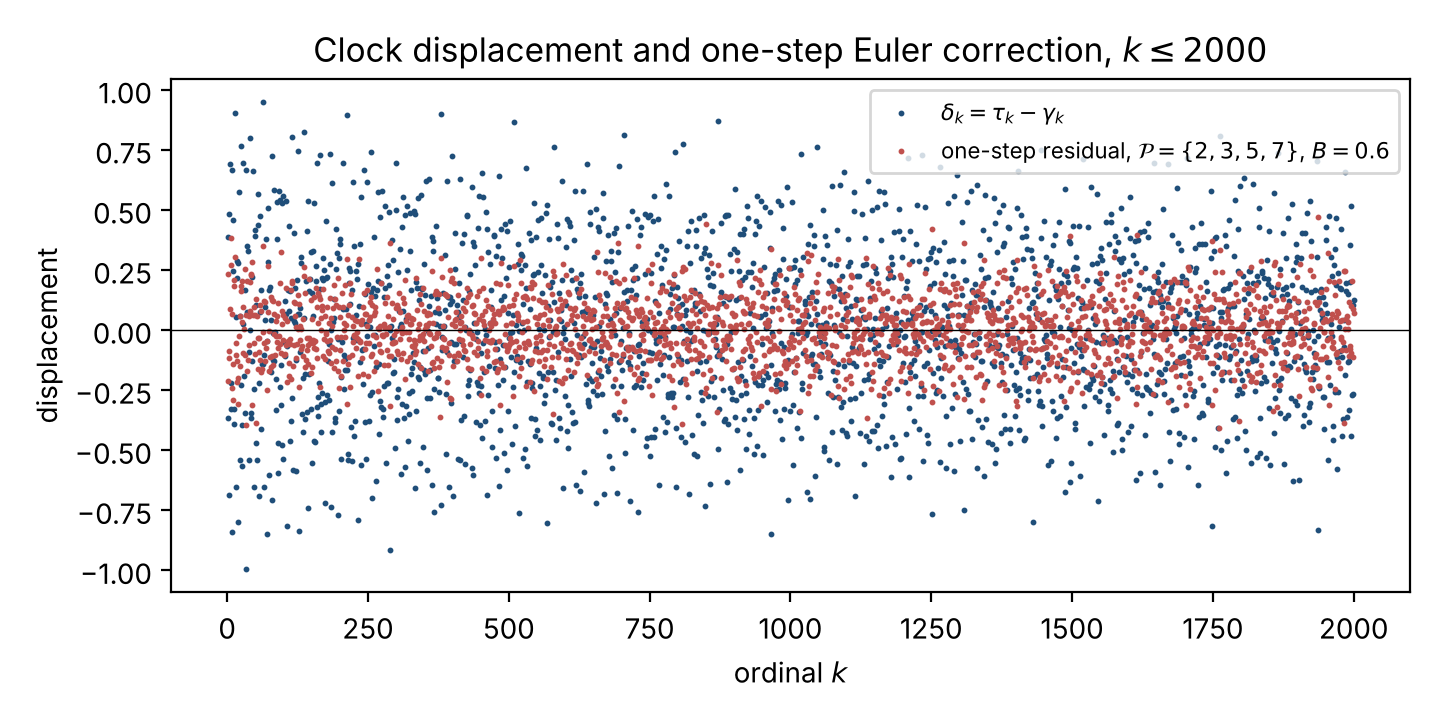
\includegraphics[width=0.86\textwidth]{fig01_displacement_first2000.png}
\caption{The displacement $\delta_k=\tau_k-\gamma_k$ of the RvM clock and the residual $\tau_k^{\PP}-\gamma_k$ of the one-step clock with $\PP=\{2,3,5,7\}$, for $k\le2000$; the correction $S_\PP(\tau_k)/\lL(\tau_k)$ is capped at $\pm B$ with $B=0.6$ (saturation, Section~\CGref{subsec:one_step_cutoff}).}
\label{fig:displacement}
\end{figure}

\subsection{Direct defects (Theorem B)}
\label{subsec:direct_defects}
For $T\in\{2^{14},2^{16},2^{18},2^{19}\}$ and $c\in\{\frac1{10},\frac15,\frac13,\frac12\}$ we compute $u_k(X)$ at the true ordinates with $X=T^c$ constant on $(T,2T]$; the windows contain $21\,519$, $100\,536$, $459\,982$ and $977\,804$ ordinates. Smaller exponents give $X<2$ at these heights and are excluded, as in Theorem~\CGref{thm:main}.

\begin{table}[htbp]
\centering\small
\caption{Mean squares of the defect $u_k(X)$ and of the one-step residual $r_k(X)$ over $T<\gamma_k\le2T$, $X=T^c$.}
\label{tab:direct}
\begin{tabular}{rrrrrrr}
\toprule
$T$ & $c$ & $X$ & $\#\{p\le X\}$ & $\langle u_k(X)^2\rangle$ & $\langle r_k(X)^2\rangle$ & $\frac1{2\pi^2}\log\frac1c$\\
\midrule
$2^{14}$ & $1/10$ & 2.64 & 1 & 0.066738 & 0.066312 & 0.116650\\
$2^{14}$ & $1/5$ & 6.96 & 3 & 0.039487 & 0.038425 & 0.081535\\
$2^{14}$ & $1/3$ & 25.40 & 9 & 0.020174 & 0.018347 & 0.055656\\
$2^{14}$ & $1/2$ & 128.00 & 31 & 0.010929 & 0.010701 & 0.035115\\
$2^{16}$ & $1/10$ & 3.03 & 2 & 0.056337 & 0.055961 & 0.116650\\
$2^{16}$ & $1/5$ & 9.19 & 4 & 0.039588 & 0.039045 & 0.081535\\
$2^{16}$ & $1/3$ & 40.32 & 12 & 0.022282 & 0.021508 & 0.055656\\
$2^{16}$ & $1/2$ & 256.00 & 54 & 0.011533 & 0.012316 & 0.035115\\
$2^{18}$ & $1/10$ & 3.48 & 2 & 0.062696 & 0.062544 & 0.116650\\
$2^{18}$ & $1/5$ & 12.13 & 5 & 0.041377 & 0.041265 & 0.081535\\
$2^{18}$ & $1/3$ & 64.00 & 18 & 0.022737 & 0.022855 & 0.055656\\
$2^{18}$ & $1/2$ & 512.00 & 97 & 0.011983 & 0.013848 & 0.035115\\
$2^{19}$ & $1/10$ & 3.73 & 2 & 0.065599 & 0.065517 & 0.116650\\
$2^{19}$ & $1/5$ & 13.93 & 6 & 0.040530 & 0.040623 & 0.081535\\
$2^{19}$ & $1/3$ & 80.63 & 22 & 0.022911 & 0.023446 & 0.055656\\
$2^{19}$ & $1/2$ & 724.08 & 128 & 0.012187 & 0.014567 & 0.035115\\
\bottomrule
\end{tabular}
\end{table}

\begin{figure}[htbp]
\centering
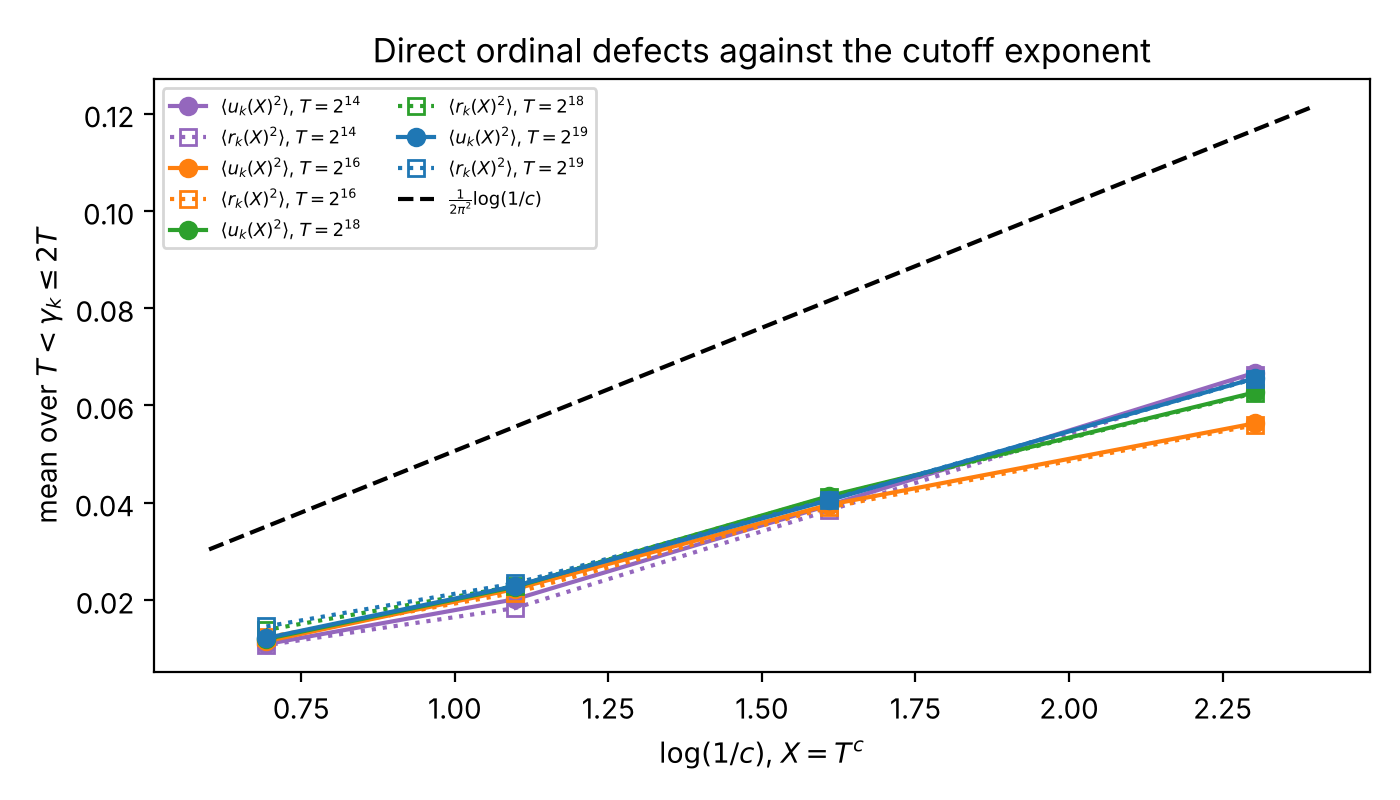
\includegraphics[width=0.86\textwidth]{fig02_direct_defects.png}
\caption{Mean square of $u_k(X)$ (filled markers) and of $r_k(X)$ (open markers) over $T<\gamma_k\le2T$ against $\log(1/c)$, $X=T^c$, for the four heights of Table~\CGref{tab:direct}; dashed: $\frac1{2\pi^2}\log(1/c)$.}
\label{fig:direct_defects}
\end{figure}

At fixed $c$ the measured means are essentially independent of $T$, as Theorem~\CGref{thm:main} requires of a bounded quantity, and they decrease monotonically in $c$. Between $c=\frac12$ and $c=\frac1{10}$ the increase of $\langle u_k^2\rangle$ at $T=2^{19}$ is $0.0534$, against $0.0815$ for the main term; at these heights the error term $O(1+\sqrt{\log(1/c)})$ is not small compared with the main term, and the data do not determine a limit at fixed $c$. The one-step residual $r_k(X)$ agrees with $u_k(X)$ to within $3\%$ for $c\le\frac15$ and exceeds it at $c=\frac12$ ($0.0146$ against $0.0122$ at $T=2^{19}$): this is the cost of evaluating $S_X$ at $\tau_k$ instead of $\gamma_k$ (Theorem~\CGref{thm:accounting}(a)).

\subsection{Exact accounting (Theorem C)}
\label{subsec:accounting_data}
For $X\in\{7,61,401,907,1999\}$ and the five windows above $k=1000$ we compute the gain $\langle s_k^2-(s_k-S_X(\tau_k))^2\rangle$, the diagonal term $D_X$ and the cross term $\Cr_X$ of \CGeqref{eq:full_factor_gain}. Table~\CGref{tab:accounting} lists three windows; Figure~\CGref{fig:accounting} shows all five.

\begin{table}[htbp]
\centering\small
\caption{Exact decomposition \CGeqref{eq:full_factor_gain} of the one-step gain into the diagonal term $D_X$ and the cross term $\Cr_X$.}
\label{tab:accounting}
\begin{tabular}{lrrrrrr}
\toprule
window of $k$ & $\langle s_k^2\rangle$ & $X$ & gain & $D_X$ & $\Cr_X$ & $v_X$\\
\midrule
$(10^3,10^4]$ & 0.085195 & 7 & 0.063224 & 0.063984 & 0.000760 & 0.066252\\
 &  & 61 & 0.075868 & 0.085258 & 0.009390 & 0.093853\\
 &  & 401 & 0.067945 & 0.097561 & 0.029616 & 0.111486\\
 &  & 907 & 0.062337 & 0.100483 & 0.038146 & 0.117730\\
 &  & 1999 & 0.055885 & 0.101829 & 0.045944 & 0.123202\\
\addlinespace
$(10^5,5\cdot10^5]$ & 0.106325 & 7 & 0.064185 & 0.064201 & 0.000016 & 0.066252\\
 &  & 61 & 0.086367 & 0.086579 & 0.000212 & 0.093853\\
 &  & 401 & 0.093276 & 0.096932 & 0.003657 & 0.111486\\
 &  & 907 & 0.092779 & 0.099690 & 0.006911 & 0.117730\\
 &  & 1999 & 0.091379 & 0.101921 & 0.010542 & 0.123202\\
\addlinespace
$(10^6,K]$ & 0.113224 & 7 & 0.064441 & 0.064444 & 0.000003 & 0.066252\\
 &  & 61 & 0.087434 & 0.087478 & 0.000044 & 0.093853\\
 &  & 401 & 0.098011 & 0.098495 & 0.000483 & 0.111486\\
 &  & 907 & 0.098607 & 0.101389 & 0.002782 & 0.117730\\
 &  & 1999 & 0.098325 & 0.103474 & 0.005149 & 0.123202\\
\bottomrule
\end{tabular}
\end{table}

\begin{figure}[htbp]
\centering
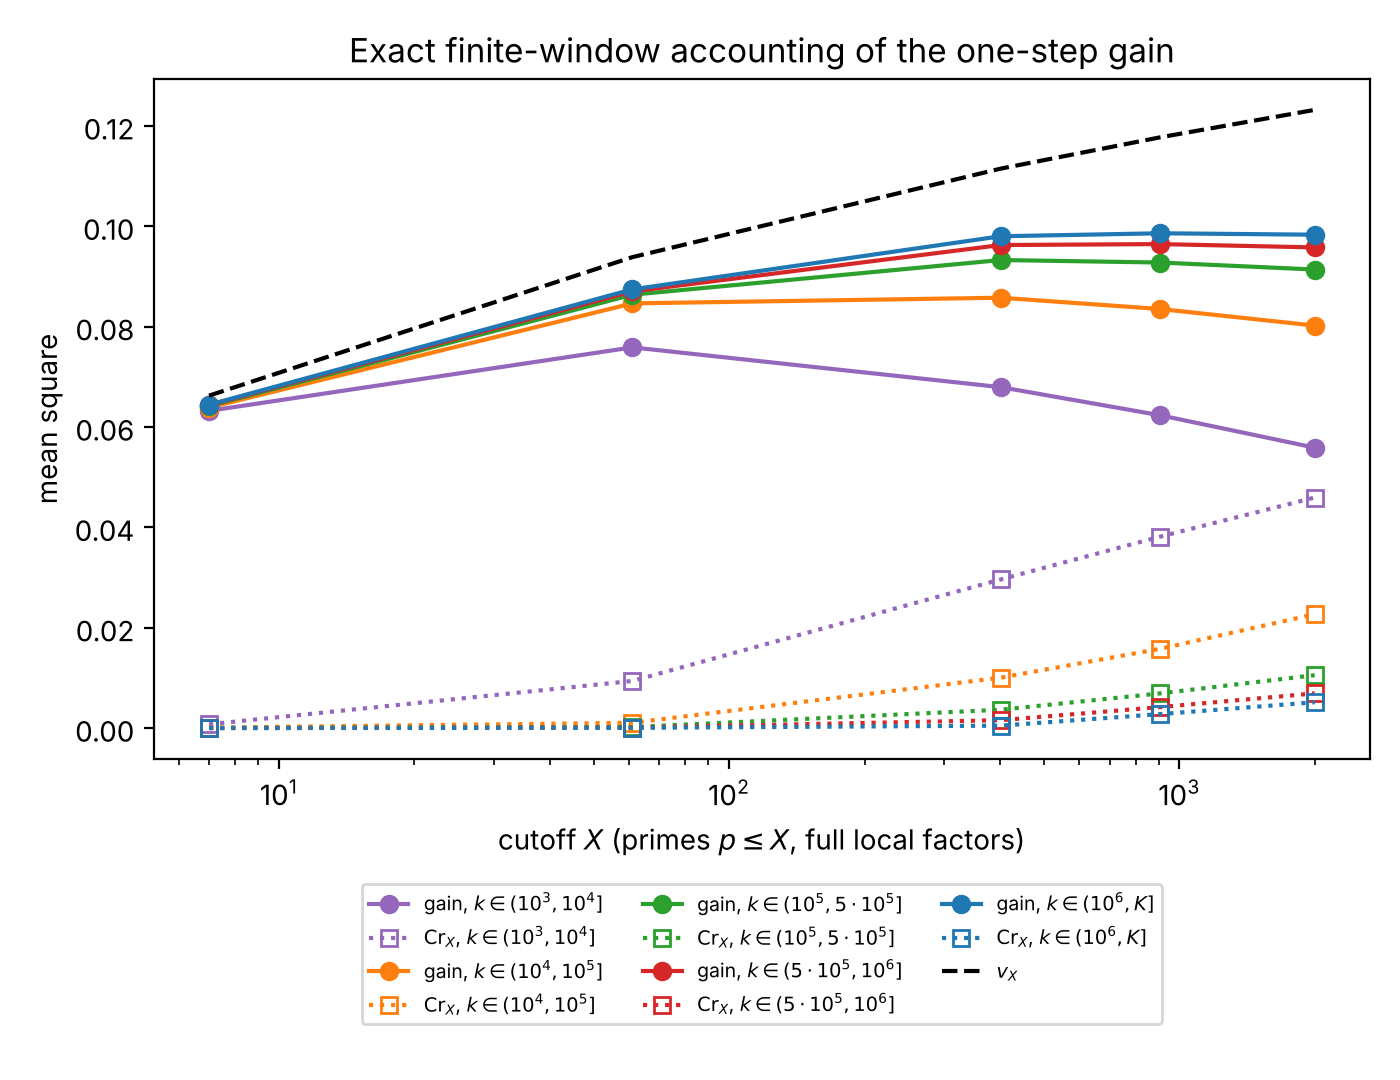
\includegraphics[width=0.86\textwidth]{fig03_accounting.png}
\caption{Gain of the one-step clock (filled markers) and cross term $\Cr_X$ (open markers) against the cutoff $X$, for five windows of ordinals; dashed: $v_X$.}
\label{fig:accounting}
\end{figure}

The diagonal term $D_X$ increases with $X$ in every window and stays below $v_X$; the cross term $\Cr_X$ grows with $X$ at fixed height and decreases with the height at fixed $X$. The gain is therefore maximal at a cutoff that increases with the height: $X=61$ on $(10^3,10^4]$, between $401$ and $1999$ on $(10^5,5\cdot10^5]$, and near $907$ on $(10^6,K]$. No parameter is fitted, and the identity gain $=D_X-\Cr_X$ is exact.

\subsection{The one-step clock against the cutoff}
\label{subsec:one_step_cutoff}
For comparison with \cite{FrancaLeClair2014,LeClair2021} we also report the root mean square and the maximum of $\tau_k^X-\gamma_k$ for $40$ cutoffs $2\le X\le1999$ (Figure~\CGref{fig:rms_cutoff}) and for five rules, with saturation $\tau_k-\sgn(y_k)\min(|y_k|,B)$, $y_k=S_X(\tau_k)/\lL(\tau_k)$, where indicated (Table~\CGref{tab:methods}, Figure~\CGref{fig:max_window}). The minimizing cutoff increases from $7$ on $(0,10^3]$ to $907$ on $(10^6,K]$, in agreement with the accounting above, and a least-squares fit $\log X_{\rm opt}=\theta_{\rm fit}\log(\tau/2\pi)$ over the five upper windows gives $\theta_{\rm fit}=0.5744$. This exponent is exploratory: the curves are flat near the minimum (in the top window the root mean square is $0.06447$ at $X=701$, $0.06427$ at $X=907$ and $0.06428$ at $X=1009$), and it is not asserted to be asymptotically optimal. At these heights the minimizing cutoff lies beyond the onset $X\approx(\tau/2\pi)^{1/2}$ of the cross term of the primes (Section~\CGref{subsec:onset}), where the gain of further primes is offset by the resonant pairs; $\theta_{\rm fit}$ describes this finite-height balance. A large fixed cutoff is harmful at small heights: $\PP=\{p\le1999\}$ gives the residual $3.247$ at $k=1$. The largest residual for $\PP=\{2,3,5,7\}$, at $k=258\,318$, follows the close pair $\gamma_{258317}=175\,681.6491$, $\gamma_{258318}=175\,681.7159$ (normalized gap $0.109$), at which $S^*(\gamma_{258318})=1.039$, so that $S(\gamma_{258318}^+)=1.539$, and $\delta_{258318}=0.638$.

\begin{table}[htbp]
\centering\footnotesize
\caption{Root mean square, maximum of $|\tau_k^X-\gamma_k|$ and number of residuals $\ge\frac12$ over all $K$ ordinates, and the same quantities in the top window $(10^6,K]$.}
\label{tab:methods}
\setlength{\tabcolsep}{4pt}
\begin{tabular}{lrrrrrr}
\toprule
rule & RMS & max & $\#\ge\frac12$ & RMS, top & max, top & $\#\ge\frac12$, top\\
\midrule
bare clock $\tau_k$ & 0.188066 & 0.993711 & 11589 & 0.178900 & 0.717359 & 2971\\
$\mathcal P=\{2,3,5,7\}$, $B=0.6$ & 0.120691 & 0.522347 & 1 & 0.117413 & 0.489293 & 0\\
$\mathcal P=\{p\le61\}$, $B=0.6$ & 0.085635 & 0.457259 & 0 & 0.085354 & 0.400144 & 0\\
$\mathcal P=\{p\le1999\}$, no saturation & 0.070757 & 3.247397 & 156 & 0.064897 & 0.528267 & 7\\
$X_k=\max(7,(\tau_k/2\pi)^{0.57})$, $B=0.6$ & 0.066608 & 0.513886 & 2 & 0.064259 & 0.513886 & 1\\
\bottomrule
\end{tabular}
\end{table}

\begin{figure}[htbp]
\centering
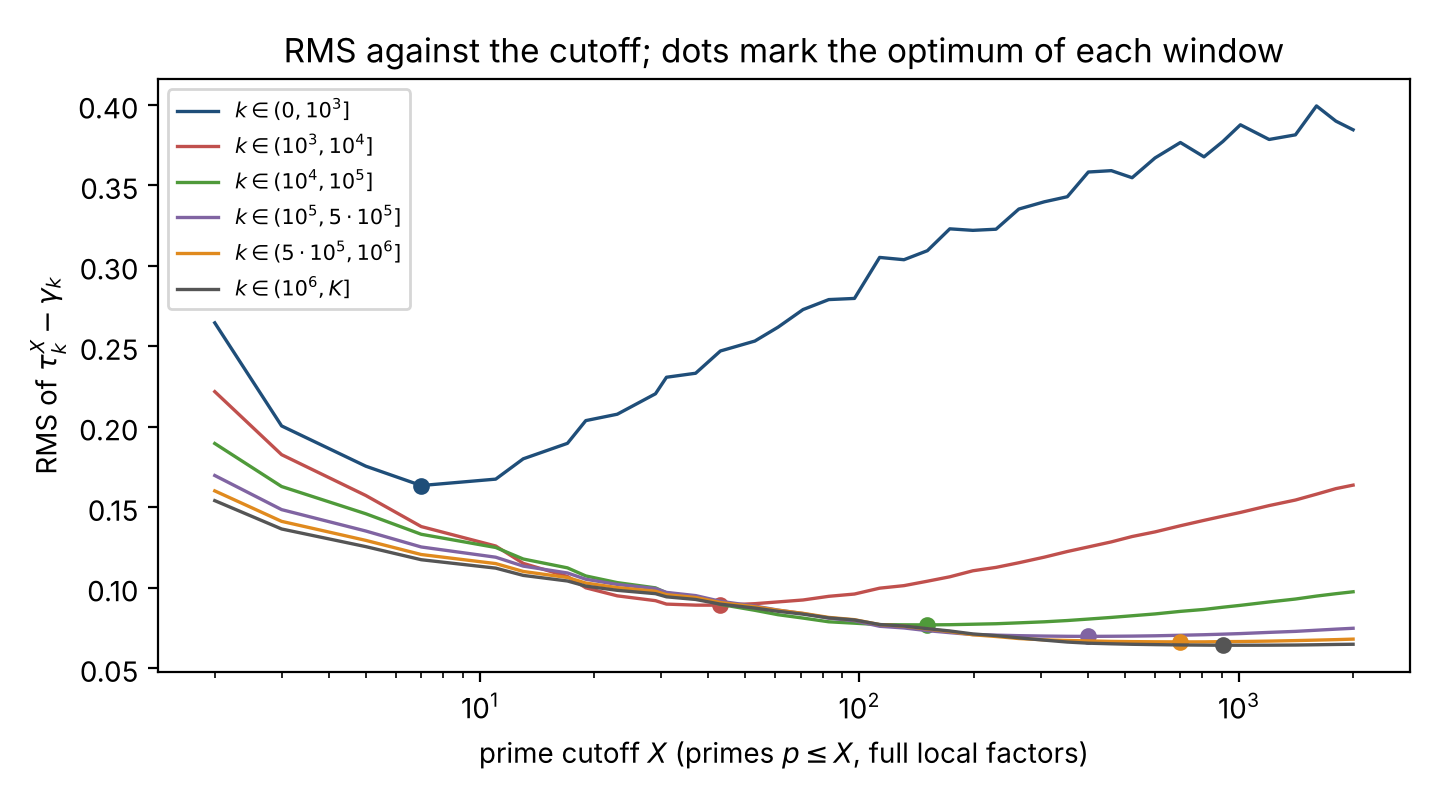
\includegraphics[width=0.86\textwidth]{fig04_rms_vs_cutoff.png}
\caption{Root mean square of $\tau_k^X-\gamma_k$ (no saturation) against the cutoff $X$, by window of ordinals; dots mark the minimum in each window.}
\label{fig:rms_cutoff}
\end{figure}

\begin{figure}[htbp]
\centering
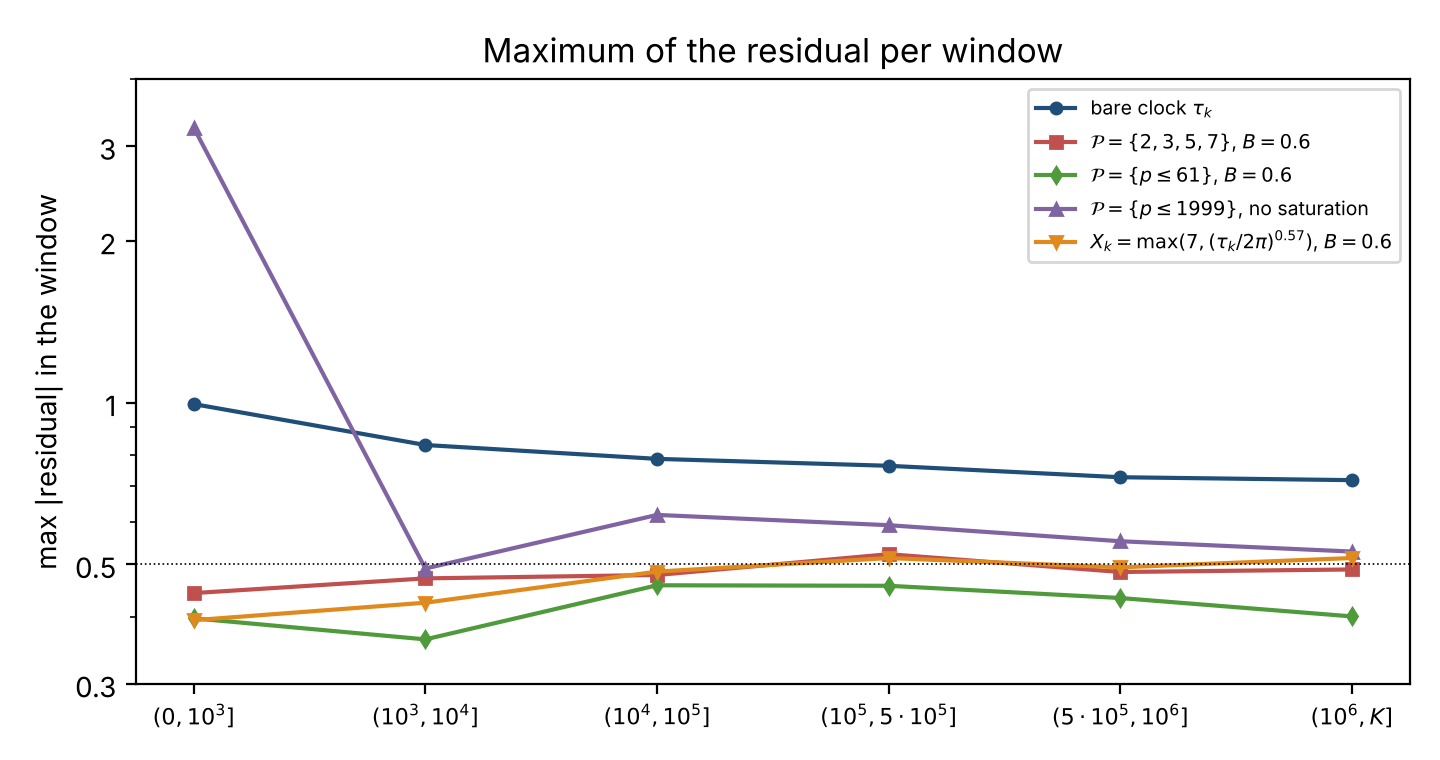
\includegraphics[width=0.86\textwidth]{fig05_max_by_window.png}
\caption{Maximum of $|\tau_k^X-\gamma_k|$ in each window of ordinals for the five rules of Table~\CGref{tab:methods}, logarithmic scale; dotted: $\frac12$. The value $3.247$ of the fixed set $\{p\le1999\}$ in the first window occurs at $k=1$.}
\label{fig:max_window}
\end{figure}

\subsection{Transport and the Newton term (Theorem D)}
\label{subsec:transport_data}
Table~\CGref{tab:transport} decomposes the residual \CGeqref{eq:r_decomposition} on the window $T=2^{19}$ of Table~\CGref{tab:direct} (all $977\,804$ ordinates, full local factors). The identity $r_k=u_k+\mathfrak t_k+\chi_k$ holds to $2\cdot10^{-16}$, and $0\le\chi_k\le6.8\cdot10^{-8}$ up to rounding.

\begin{table}[htbp]
\centering\footnotesize
\caption{Transport term and Newton term of the one-step clock over $2^{19}<\gamma_k\le2^{20}$, $X=T^c$: mean squares, the correlation of $u_k(X)$ with $\mathfrak t_k(X)$, the root mean square of $S_X'(\tau_k)/\lL(\tau_k)$, and the proportion of indices with $F_X'(\tau_k)<0$.}
\label{tab:transport}
\setlength{\tabcolsep}{3.5pt}
\begin{tabular}{lrrrrrrrr}
\toprule
$c$ & $X$ & $\langle u_k^2\rangle$ & $\langle\mathfrak t_k^2\rangle$ & corr$(u_k,\mathfrak t_k)$ & $\langle r_k^2\rangle$ & $\langle(y_kS_X'(\tau_k))^2\rangle$ & RMS $\frac{S_X'(\tau_k)}{\lL(\tau_k)}$ & $F_X'(\tau_k)<0$\\
\midrule
$1/5$ & 13.93 & 0.040530 & 0.004905 & $-0.171$ & 0.040623 & 0.003559 & 0.225 & $0.002\%$\\
$1/3$ & 80.63 & 0.022911 & 0.011391 & $-0.336$ & 0.023446 & 0.014386 & 0.361 & $0.27\%$\\
$1/2$ & 724.08 & 0.012187 & 0.018283 & $-0.533$ & 0.014567 & 0.046866 & 0.525 & $2.7\%$\\
\bottomrule
\end{tabular}
\end{table}

The transport is smaller than $c^2\log\log T$ ($=0.103$, $0.287$, $0.644$) by factors $21$--$35$, and it is anticorrelated with $u_k(X)$, increasingly with $c$; this is why $\langle r_k^2\rangle$ exceeds $\langle u_k^2\rangle$ by only $0.0001$--$0.0024$. The root mean square of $S_X'/\lL$ is close to $c$, as in Remark~\CGref{rem:newton}, and the Newton term $y_kS_X'(\tau_k)$ has correlation $0.66$--$0.77$ with $-\mathfrak t_k(X)$; at $c=\frac12$ it overestimates the transport, and the denominator of \CGeqref{eq:newton_exact} matters.

\subsection{Onset of the cross term}
\label{subsec:onset}
Table~\CGref{tab:onset} gives $\Cr_X$ on the top window $(10^6,K]$, where $\tau_k/2\pi$ runs over $[95\,536,180\,241]$, for the full Euler phase and for its prime part $S^{(1)}_X(t)=-\frac1\pi\sum_{p\le X}p^{-1/2}\sin(t\log p)$, with $\Cr^{(1)}_X=\langle S^{(1)}_X(\tau_k)^2\rangle-\frac12\sum_{p\le X}a_p^2$.

\begin{table}[htbp]
\centering\small
\caption{Cross term at the clock points on $(10^6,K]$; $(\tau_{\min}/2\pi)^{1/2}=309.1$.}
\label{tab:onset}
\begin{tabular}{rrrr}
\toprule
$X$ & $\#\{p\le X\}$ & $\Cr_X$ & $\Cr^{(1)}_X$\\
\midrule
100 & 25 & 0.000083 & 0.000000\\
200 & 46 & 0.000149 & 0.000000\\
300 & 62 & 0.000186 & 0.000000\\
316 & 65 & 0.000195 & 0.000004\\
350 & 70 & 0.000248 & 0.000048\\
400 & 78 & 0.000449 & 0.000235\\
500 & 95 & 0.001107 & 0.000857\\
700 & 125 & 0.002056 & 0.001761\\
907 & 155 & 0.002782 & 0.002447\\
1200 & 196 & 0.003608 & 0.003210\\
1999 & 303 & 0.005149 & 0.004662\\
\bottomrule
\end{tabular}
\end{table}

$\Cr^{(1)}_X$ vanishes to six decimals until $X^2$ reaches $\tau_{\min}/2\pi$ and then grows. For $X=1999$ the $91\,809$ ordered pairs of primes split into the $7\,807$ pairs with $pq\in[\tau_{\min}/2\pi,\tau_{\max}/2\pi]$, which contribute $0.004657$, and the others, which contribute $0.000005$. The full Euler phase has earlier resonances, from products of prime powers in the same range, with smaller weights. This is the mechanism of Proposition~\CGref{prop:cross_term}: the phase $\omega\tau_x/2\pi$ with $\omega=\log n$ is stationary in the sense of the Poisson summation formula exactly at $\tau_x=2\pi n$. A stationary-phase evaluation (heuristic: endpoint terms and the variation of the amplitude are neglected) at $x_0$ with $\tau_{x_0}=2\pi n$, where $\omega\tau_{x_0}/2\pi-x_0=n-\frac{11}8$ and the second derivative of the phase is $-2\pi/(\tau\log^2(\tau/2\pi))$, gives $\sum_{k\in I}e^{i\tau_k\log n}\approx-\sqrt n\log n$, hence a contribution $\log(pq)/(2\pi^2\#I)$ of each resonant ordered pair to $\Cr^{(1)}_X$. Summed over the $7\,807$ pairs this is $0.004663$, against $0.004657$ measured.


\subsection{A comparison construction and its Newton residual}
\label{subsec:zcasanya_data}
The array \texttt{zCasanya} is the clock corrected by three Newton steps \CGeqref{eq:newton_iteration} with the sharp phase $S_{\le X}$ of \CGeqref{eq:sharp_def} and dyadic cutoffs
\begin{equation}
X_j(k)=\min\bigl(\bar X_j,\max(8,\lfloor2^{\lfloor\log_2\tau_k\rfloor/2}\rfloor)\bigr),\qquad(\bar X_1,\bar X_2,\bar X_3)=(8,8,512).
\label{eq:dyadic_cutoffs}
\end{equation}
The sequence $(8,8,512)$ was selected among $836$ nondecreasing sequences of one to four cutoffs from $\{8,32,128,512,2048,8192\}$, by the root mean square against the ordinates on $k\le1\,400\,736$ (tuning on the first $40\%$ of the indices, selection on the next $30\%$); the indices $1\,400\,737\le k\le2\,001\,052$ were not used until the selection was frozen and are not used for any choice in this section. The construction itself reads no ordinate. The program \texttt{opc\_rebuild\_zcasanya\_v15.py} recomputes the array from the clock alone and reproduces it to $9.3\cdot10^{-10}$ ($1.8\cdot10^{-9}$ in units of zeros), with the same $962$ inversions $x_{k+1}\le x_k$.

Over all $K$ ordinates (program \texttt{opc\_task1\_newton\_residual.py}) its root mean square in height is $0.04399$ (bare clock $0.18807$, Table~\CGref{tab:methods}), and the ordinal residual
\begin{equation}
\mathsf r_k=\NO(\gamma_k)-\NO(x_k)
\label{eq:ordinal_residual}
\end{equation}
has root mean square $0.0770$ and autocorrelations $-0.633$, $+0.316$, $-0.196$ at lags $1,2,3$. The residual $\mathsf E_k(x^{(3)}_k)$ of the equation \CGeqref{eq:equation_residual}, with the third cutoff, has root mean square $0.1056$ and explains $16.9\%$ of the variance of $\mathsf r_k$ (squared correlation). Solving the truncated equation exactly with the same cutoffs (Newton's method with the true derivative from $x^{(3)}_k$, converged at $99.996\%$ of the indices; the others keep $x^{(3)}_k$) changes the autocorrelations to $-0.478$, $+0.085$, $-0.032$, removes all inversions, and raises the root mean square in height to $0.04560$; the root mean square of the second differences $\mathsf r_{k+2}-\mathsf r_k$ rises from $0.0900$ to $0.1093$, that of the first differences is unchanged ($0.1391$, $0.1389$). Table~\CGref{tab:newton_residual_spectra} and Figure~\CGref{fig:newton_residual_spectra} give the periodograms by dyadic block of height: the spectra of $\mathsf r_k$ and $\mathsf E_k$ have correlation $0.96$--$0.98$, and the step of the spectrum of $\mathsf r_k$ above the folded edge $1-c$ of Remark~\CGref{rem:nyquist} disappears with the exact root. The alternation that remains at lag $1$ is the folded defect of the prime powers above the final cutoff.

\begin{table}[htbp]
\centering\footnotesize
\caption{Periodograms of the ordinal residual $\mathsf r_k$ of \texttt{zCasanya}, of the equation residual $\mathsf E_k$, and of $\mathsf r_k$ for the exact root with the same cutoffs, by block of $\tau_k$: median third cutoff $X_3$, folded edge $1-\log X_3/\log(\tau/2\pi)$ at the median height, peak frequency $\alpha$, fraction of the power in $0.4\le\alpha\le0.5$, and correlation of the logarithmic spectra of $\mathsf r_k$ and $\mathsf E_k$.}
\label{tab:newton_residual_spectra}
\setlength{\tabcolsep}{3pt}
\begin{tabular}{lrrrrrrrrrr}
\toprule
$\tau_k\in$ & $n$ & $X_3$ & $1-c$ & peak $\mathsf r$ & peak $\mathsf E$ & peak exact & band $\mathsf r$ & band $\mathsf E$ & band exact & corr\\
\midrule
$(2^{16},2^{17}]$ & 100\,536 & 256 & 0.426 & 0.491 & 0.488 & 0.474 & 0.588 & 0.432 & 0.384 & 0.980\\
$(2^{17},2^{18}]$ & 215\,532 & 362 & 0.431 & 0.453 & 0.454 & 0.476 & 0.584 & 0.430 & 0.386 & 0.984\\
$(2^{18},2^{19}]$ & 459\,982 & 512 & 0.435 & 0.498 & 0.498 & 0.486 & 0.577 & 0.424 & 0.391 & 0.983\\
$(2^{19},2^{20}]$ & 977\,804 & 512 & 0.469 & 0.471 & 0.471 & 0.449 & 0.575 & 0.372 & 0.417 & 0.975\\
$(2^{20},\tau_K]$ & 161\,121 & 512 & 0.483 & 0.469 & 0.494 & 0.470 & 0.591 & 0.352 & 0.441 & 0.964\\
\bottomrule
\end{tabular}
\end{table}

\begin{figure}[htbp]
\centering
\includegraphics[width=0.86\textwidth]{fig09_newton_residual_spectra.png}
\caption{Periodograms of the ordinal residual (r), of the equation residual (E3, that is $\mathsf E_k$ with the third cutoff) and of the ordinal residual of the exact root (r\_exact), by block of $\tau_k$; dotted: folded edge $1-c$; dashed: $1-c\pm\alpha_q$, $q\in\{2,3,4,5,7,8\}$.}
\label{fig:newton_residual_spectra}
\end{figure}

\subsection{Certified roots and continuation on the untouched indices}
\label{subsec:rule_data}
Table~\CGref{tab:rule} compares the rule of Section~\CGref{subsec:rule} with \texttt{zCasanya} on the $600\,316$ untouched indices $1\,400\,737\le k\le2\,001\,052$, all errors measured against the ordinates (program \texttt{opc\_task3\_analytic\_rule.py}). Stage A has $X^{\rm A}_k=16$ at every index of this range, and $F_{\le16}=k-\frac12$ is bracketed and solved by bisection at all of them. The continuation is accepted at $\ge99.98\%$ of the indices at each of the six levels, for both rules. For R2 the median of $c_{\rm G}$ is $0.696$ (deciles $0.694$ and $0.699$), so $99.94\%$ of the indices end beyond the Nyquist cutoff. The model value of Heuristic~\CGref{heur:gaussian_cutoff} is $\hat\sigma=0.269$ (median), against $0.199$ for the root mean square of $\lL(\tau_k)(x^{\rm A}_k-\gamma_k)$. The acceptance condition is checked at five points of the segment between consecutive roots, not by interval arithmetic.

\begin{table}[htbp]
\centering\footnotesize
\caption{Untouched indices $1\,400\,737\le k\le2\,001\,052$: errors $x_k-\gamma_k$ (root mean square, $99\%$ quantile, maximum, proportion of indices improved over the clock), the ordinal residual $\mathsf r_k$ (root mean square, root mean square of first differences, autocorrelations at lags $1,2$), inversions, fraction of the periodogram of $\mathsf r_k$ in $0.4\le\alpha\le0.5$, and the walk: $|\mathscr C(x)-\mathscr C(\gamma)|$ over the range and $\max_j|\mathscr P_j(x)-\mathscr P_j(\gamma)|$.}
\label{tab:rule}
\scriptsize\setlength{\tabcolsep}{2.4pt}
\begin{tabular}{lrrrrrrrrrrrr}
\toprule
method & RMS & p99 & max & impr. & RMS $\mathsf r$ & gap & ac1 & ac2 & inv. & band & centroid & walk max\\
\midrule
clock $\tau_k$ & 0.1774 & 0.440 & 0.689 & --- & 0.337 & 0.409 & $+0.26$ & $+0.04$ & 0 & 0.12 & 1.11 & 2.86\\
\texttt{zCasanya} & 0.0406 & 0.116 & 0.313 & 86.9\% & 0.077 & 0.140 & $-0.64$ & $+0.33$ & 274 & 0.58 & 14.72 & 29.80\\
Stage A ($X=16$) & 0.1046 & 0.257 & 0.410 & 69.2\% & 0.199 & 0.347 & $-0.52$ & $-0.16$ & 0 & 0.32 & 0.92 & 2.05\\
R1 (to Nyquist) & 0.0473 & 0.123 & 0.284 & 85.0\% & 0.090 & 0.158 & $-0.54$ & $+0.17$ & 0 & 0.47 & 14.08 & 26.71\\
R2 (to $c_{\rm G}$) & \textbf{0.0331} & \textbf{0.081} & \textbf{0.275} & \textbf{88.4\%} & \textbf{0.063} & \textbf{0.106} & $-0.40$ & $-0.01$ & 0 & 0.35 & 7.75 & 17.58\\
\bottomrule
\end{tabular}
\end{table}

\begin{figure}[htbp]
\centering
\includegraphics[width=0.86\textwidth]{fig11_test_set_comparison.png}
\caption{Untouched indices: periodograms of the ordinal residual and $|\mathscr P_j(x)-\mathscr P_j(\gamma)|$ along the range, for \texttt{zCasanya}, Stage A and the rules R1 and R2 of Section~\CGref{subsec:rule}.}
\label{fig:test_set_comparison}
\end{figure}

R2 is better than the selected comparison in every measure that refers to the ordinates: root mean square $-18\%$, $99\%$ quantile $-30\%$, error of the gaps $-24\%$, no inversion, the alternation at lag $2$ removed, and half the drift of the walk. R1 stops at the Nyquist cutoff and keeps the alternation (Remark~\CGref{rem:nyquist}). The drift of the walk is far from that of the ordinates for all corrected constructions; Section~\CGref{subsec:walk_data} identifies its source.

\subsection{Continuation beyond the Nyquist cutoff}
\label{subsec:beyond_nyquist}
The continuation does not use $X\le T^{1/2}$. Table~\CGref{tab:beyond_nyquist} continues the root of Stage A to the fixed exponents $c\in\{0.85,1.00,1.15,1.30\}$ of $\tau_k/2\pi$, with eight geometric levels, on the block $1\,636\,863\le k\le1\,646\,862$ of the untouched range (programs \texttt{opc\_task4\_selfconsistent\_cutoff.py} and \texttt{opc\_task4\_fit\_b3.py}). The continuation is accepted at $\ge99.95\%$ of the indices at every level; fewer than $0.1\%$ of the indices stop below the target cutoff. On six blocks of $10\,000$ indices spread over the untouched range the root mean square is $0.0266$ for $c=0.85$ and $0.0210$ for $c=1.00$, against $0.0408$ for \texttt{zCasanya} and $0.0331$ for R2 (program \texttt{opc\_task4\_eval.py}).

\begin{table}[htbp]
\centering\footnotesize
\caption{Block $1\,636\,863\le k\le1\,646\,862$: errors against the ordinates, ordinal residual, inversions and walk ($|\mathscr P(x)-\mathscr P(\gamma)|$ at the end of the block and its maximum), for the clock, \texttt{zCasanya}, R2 and the continuation to $(\tau_k/2\pi)^c$.}
\label{tab:beyond_nyquist}
\setlength{\tabcolsep}{3.2pt}
\begin{tabular}{lrrrrrrrrrr}
\toprule
method & RMS & mean square & p99 & max & gap & ac1 & ac2 & inv. & walk end & walk max\\
\midrule
clock $\tau_k$ & 0.17770 & $3.158\cdot10^{-2}$ & 0.4424 & 0.589 & 0.4093 & $+0.263$ & $+0.039$ & 0 & 1.868 & 2.538\\
\texttt{zCasanya} & 0.04028 & $1.623\cdot10^{-3}$ & 0.1147 & 0.243 & 0.1380 & $-0.630$ & $+0.322$ & 6 & 2.204 & 3.145\\
R2 & 0.03323 & $1.104\cdot10^{-3}$ & 0.0822 & 0.176 & 0.1058 & $-0.408$ & $-0.013$ & 0 & 1.151 & 1.497\\
$c=0.85$ & 0.02657 & $7.062\cdot10^{-4}$ & 0.0644 & 0.188 & 0.0830 & $-0.356$ & $-0.045$ & 0 & 0.982 & 1.477\\
$c=1.00$ & 0.02124 & $4.510\cdot10^{-4}$ & 0.0516 & 0.173 & 0.0660 & $-0.340$ & $-0.057$ & 0 & 0.418 & 1.092\\
$c=1.15$ & 0.01644 & $2.702\cdot10^{-4}$ & 0.0414 & 0.209 & 0.0505 & $-0.311$ & $-0.064$ & 0 & 0.488 & 0.695\\
$c=1.30$ & 0.01276 & $1.628\cdot10^{-4}$ & 0.0318 & 0.186 & 0.0396 & $-0.341$ & $-0.050$ & 0 & 0.028 & 0.750\\
\bottomrule
\end{tabular}
\end{table}

The mean square falls with $c$, but more slowly as $c$ grows: its slopes against $\log c$ are $-1.57\cdot10^{-3}$, $-1.29\cdot10^{-3}$, $-0.88\cdot10^{-3}$ on the three intervals. The straight line through $c=1.00$ and $c=1.15$ predicts $1.12\cdot10^{-4}$ at $c=1.30$; the observed value is $1.63\cdot10^{-4}$, so the linear extrapolation to zero error near $c=1.4$ is ruled out. A quadratic in $\log c$ through the four points has its minimum $3.5\cdot10^{-5}$ (root mean square $0.006$) at $c\approx1.8$; with four points this is a description of the curve, not an estimate of a limit. The maximum error does not decrease ($0.17$--$0.21$). The cutoff $(\tau_k/2\pi)^{1.30}$ exceeds the height in the scale $\tau/2\pi$: the continuation is not limited by the range of the moment estimates of Section~\CGref{sec:main_theorem}.

\subsection{The drift of the walk}
\label{subsec:walk_data}
Over all $K$ ordinates (program \texttt{opc\_walk\_centroids\_v15.py}) the centroids \CGeqref{eq:walk_def} are
\begin{equation}
\mathscr C_K(\gamma)=0.7769+0.7678i,\qquad\mathscr C_K(\tau)=0.0416+1.7575i,\qquad\mathscr C_K(x^{\rm C})=2.7412+17.7391i
\label{eq:centroids}
\end{equation}
for the ordinates, the clock and \texttt{zCasanya} ($x^{\rm C}$). For \texttt{zCasanya}, \CGeqref{eq:angular_radial} gives $i\mathfrak A=-0.3333+14.4893i$ and $\mathfrak B=2.2977+2.4820i$ (closure $6\cdot10^{-14}$): the angular part carries $85\%$ of the imaginary part, and the radial part, of modulus $3.38$, is not negligible, because $e_k^2$ contains $\cos(\gamma_k\log(n_1/n_2))$, which resonates with $e^{i\gamma_k}$ when $n_2/n_1\approx e$. Relative to the clock (program \texttt{opc\_task2\_quotient\_drift.py}, no ordinate used) the expansion \CGeqref{eq:walk_clock_expansion} gives
\begin{equation}
\begin{split}
&\mathscr C_K(x^{\rm C})-\mathscr C_K(\tau)=2.700+15.982i,\\
&\text{linear part }-2.236-5.557i,\qquad\text{quadratic part }5.242+20.593i,
\end{split}
\label{eq:drift_parts}
\end{equation}
and for the one-step model $\mathsf y_k=S_{\le X_3(k)}(\tau_k)/\lL(\tau_k)$, which has correlation $0.941$ with $\mathsf y_k=\tau_k-x^{\rm C}_k$, identity \CGeqref{eq:product_quotient} holds to $3\cdot10^{-16}$ and splits the quadratic part $7.057+16.332i$ into products $-2.322+10.717i$ and quotients $9.379+5.615i$. The slow quotient modes, $|\upsilon_{n_1,n_2}|\le0.02$, give $8.194+10.677i$. One pair dominates (Table~\CGref{tab:quotient_pairs}): $(71,193)$, with $\upsilon=-1.03\cdot10^{-5}$ and contribution $7.168+12.006i$, of modulus $14.0$ against $16.2$ for the whole drift. The next pairs are $(7,19)$, $(2,5)$, $(3,8)$, $(4,11)$; four of the five largest pairs are convergents \CGeqref{eq:e_convergents}. The slow shape of the excursion of the walk in Figure~\CGref{fig:walk_drift} is the oscillation of the pair $(71,193)$, of period $\approx1.1\cdot10^6$ indices. Since $|\mathscr C_K(\tau)-\mathscr C_K(\gamma)|=1.23$, the same resonance separates the corrected points from the ordinates: in the walk of the zeros it is compensated, in the truncated construction it is not.

\begin{table}[htbp]
\centering\small
\caption{The largest contributions $\mathscr R_{n_1,n_2}$ \CGeqref{eq:quotient_contribution} of quotient pairs to the drift of \texttt{zCasanya}, with $\upsilon_{n_1,n_2}$ and the period \CGeqref{eq:quotient_period} at $T=5\cdot10^5$.}
\label{tab:quotient_pairs}
\begin{tabular}{rrrrrr}
\toprule
$n_1$ & $n_2$ & $\upsilon_{n_1,n_2}$ & $\Re\mathscr R$ & $\Im\mathscr R$ & period\\
\midrule
71 & 193 & $-1.031\cdot10^{-5}$ & 7.168 & 12.006 & $1.09\cdot10^6$\\
7 & 19 & $1.471\cdot10^{-3}$ & 1.112 & $-1.562$ & 7\,670\\
2 & 5 & $8.37\cdot10^{-2}$ & 0.276 & $-0.584$ & 135\\
3 & 8 & $1.917\cdot10^{-2}$ & $-0.114$ & $-0.320$ & 589\\
4 & 11 & $-1.160\cdot10^{-2}$ & 0.309 & 0.069 & 973\\
163 & 443 & $1.804\cdot10^{-4}$ & $-0.042$ & 0.243 & 62\,542\\
29 & 79 & $-2.152\cdot10^{-3}$ & $-0.202$ & 0.072 & 5\,244\\
113 & 307 & $5.40\cdot10^{-4}$ & 0.143 & 0.014 & 20\,894\\
\bottomrule
\end{tabular}
\end{table}

\begin{figure}[htbp]
\centering
\includegraphics[width=0.86\textwidth]{fig10_walk_drift_decomposition.png}
\caption{Cumulative drift $\mathscr C(x^{\rm C})-\mathscr C(\tau)$ of \texttt{zCasanya} relative to the clock along the indices (actual), its quadratic part (quadratic\_actual), the product and quotient parts of the one-step model (product, quotient), and the slow quotient bands $|\upsilon|\le0.02$ and $|\upsilon|\le0.1$ (slow\_0.02, slow\_0.1).}
\label{fig:walk_drift}
\end{figure}

\subsection{The corrected Gram law}
\label{subsec:gram_data}
Since all zeros of the table are simple and on the critical line \cite{PlattTrudgian2021}, the corrected Gram law $Z(\bar x_{k-1})Z(\bar x_k)<0$ holds exactly when $(\bar x_{k-1},\bar x_k)$ contains an odd number of ordinates. Table~\CGref{tab:gram_law} gives, for the zero-free constructions (program \texttt{opc\_separation\_v15.py}), the proportion of indices at which the law holds, the proportion at which the hypotheses \CGeqref{eq:local_separation} of Theorem~\CGref{thm:local_separation} hold with $\mathsf h=\mathsf u/\lL(\tau_k)$, and the proportion of small gaps $\lL(\tau_k)\min(x_k-x_{k-1},x_{k+1}-x_k)\le2\mathsf u$, which is computable without zeros. For the clock the midpoints are the Gram points up to $O(\tau_k^{-1})$, and the law is Gram's law.

\begin{table}[htbp]
\centering\footnotesize
\caption{Corrected Gram law and local separation: proportion of indices with the law, with exactly one ordinate between consecutive midpoints, with the hypotheses of Theorem~\CGref{thm:local_separation} for $\mathsf u=0.10,0.15,0.20$, and with a gap $\le2\mathsf u$ in units of zeros for $\mathsf u=0.20$.}
\label{tab:gram_law}
\setlength{\tabcolsep}{3pt}
\begin{tabular}{llrrrrrr}
\toprule
indices & construction & law & one ordinate & sep.\ $0.10$ & sep.\ $0.15$ & sep.\ $0.20$ & gap $\le0.40$\\
\midrule
all $K$ & clock (Gram's law) & 0.7643 & 0.7629 & 0.012 & 0.039 & 0.087 & 0\\
 & \texttt{zCasanya} & 0.9968 & 0.9968 & 0.616 & 0.843 & 0.857 & 0.121\\
\addlinespace
untouched & clock (Gram's law) & 0.7570 & 0.7555 & 0.012 & 0.038 & 0.084 & 0\\
 & \texttt{zCasanya} & 0.9968 & 0.9968 & 0.632 & 0.852 & 0.879 & 0.091\\
 & Stage A & 0.9772 & 0.9765 & 0.076 & 0.202 & 0.365 & 0\\
 & R1 & 0.99928 & 0.99928 & 0.501 & 0.788 & 0.931 & 0.002\\
 & R2 & 0.99981 & 0.99981 & 0.751 & 0.969 & 0.940 & 0.059\\
\addlinespace
block & $c=0.85$ & 0.99980 & 0.99980 & 0.895 & 0.984 & 0.832 & 0.167\\
$1\,636\,863$-- & $c=1.00$ & 1 & 1 & 0.978 & 0.944 & 0.799 & 0.201\\
$1\,646\,862$ & $c=1.15$ & 1 & 1 & 0.996 & 0.921 & 0.806 & 0.193\\
 & $c=1.30$ & 1 & 1 & 0.996 & 0.915 & 0.826 & 0.174\\
\bottomrule
\end{tabular}
\end{table}

Gram's law holds at $76\%$ of the indices and the corrected Gram law at $99.98\%$ for R2 on the untouched range: the verification of Proposition~\CGref{prop:verification} with the corrected points has about $1/1300$ of the exceptions of Gram's law. On the block of Table~\CGref{tab:beyond_nyquist} the law holds at every index for $c\ge1$, and for $c=1.30$ the hypotheses of Theorem~\CGref{thm:local_separation} hold with $\mathsf u=0.10$ at $99.6\%$ of the indices: there the errors are below a tenth of a mean spacing and the computed gaps exceed a fifth of one, which certifies, index by index, the isolation of the ordinates by points computed without zeros.

%======================================================================
\section{Prime responses at the zeros and at the clock points}
\label{sec:responses}

\emph{Subsections~\CGref{subsec:landau_line}--\CGref{subsec:newton_spectrum} are unconditional. Subsection~\CGref{subsec:conditional_law} contains rigorous implications from two named hypotheses. Nothing heuristic is used; Theorems A--E do not depend on this section.}

\subsection{Fixed and slowly moving frequencies}
\label{subsec:landau_line}

\begin{theorem}[Landau's formula on the critical line]\label{thm:landau_line}
Uniformly for $t\ge2$ and integers $2\le n\le t^{1/8}$,
\begin{equation}
\sum_{0<\gamma\le t}n^{i\gamma}=-\frac t{2\pi}\frac{\Lambda(n)}{\sqrt n}+O\Bigl(\frac{t\log^2n}{\log t}+\sqrt n\log^2t\Bigr),
\label{eq:landau_line}
\end{equation}
zeros counted with multiplicity. For fixed $n$ the error is $O(t/\log t)$.
\end{theorem}

\begin{proof}
Let $\ell=\log n$. By the functional equation and $\zeta(\bar s)=\overline{\zeta(s)}$, $\rho\mapsto1-\bar\rho$ maps the zeros with $0<\gamma\le t$ onto themselves, preserving multiplicities and ordinates. Hence $\sum n^\rho=\sum n^{1-\bar\rho}$, and averaging the two expressions, $\sum_{0<\gamma\le t}n^\rho=\sqrt n\sum_{0<\gamma\le t}n^{i\gamma}\cosh((\beta-\frac12)\ell)$. Thus
\[
\sum_{0<\gamma\le t}n^{i\gamma}=\frac1{\sqrt n}\sum_{0<\gamma\le t}n^\rho-\mathcal K_n(t),\qquad\mathcal K_n(t)=\sum_{0<\gamma\le t}n^{i\gamma}\bigl(\cosh((\beta-\tfrac12)\ell)-1\bigr).
\]
The zeros with $\beta<\frac12$ correspond to those with $\beta>\frac12$, and those with $\beta=\frac12$ contribute $0$, so $|\mathcal K_n(t)|\le2\sum_{\beta>1/2}(\cosh((\beta-\frac12)\ell)-1)$. Writing $\cosh(x\ell)-1=\int_0^x\ell\sinh(\ell y)\,dy$ and exchanging the finite sum with the integral,
\[
\sum_{\substack{\beta>1/2\\0<\gamma\le t}}\bigl(\cosh((\beta-\tfrac12)\ell)-1\bigr)=\int_0^{1/2}\ell\sinh(\ell y)\,N^+(\tfrac12+y,t)\,dy\ll t\log t\cdot\ell\int_0^\infty\sinh(\ell y)e^{-ay}dy,
\]
with $a=\frac14\log t$, by Theorem~\CGref{thm:known_density}. For $\ell\le a/2$ the last integral is $\ell/(a^2-\ell^2)\le\frac43\ell/a^2$, so $\mathcal K_n(t)\ll t\ell^2/\log t$. Theorem~\CGref{thm:known_landau} now gives $n^{-1/2}\sum n^\rho=-\frac t{2\pi}\Lambda(n)n^{-1/2}+O(\sqrt n\log(2nt)\log\log(3n))$, and $\log(2nt)\log\log(3n)\ll\log^2t$ for $n\le t^{1/8}$.
\end{proof}

The symmetry removes the term linear in $\beta-\frac12$; Selberg's estimate then bounds the quadratic remainder. Without the symmetry one needs $\sum_{0<\gamma\le t}|\beta-\frac12|=o(t)$, which is not known.

\begin{lemma}\label{lem:clock_equidistribution}
For fixed real $\omega\ne0$, $\sum_{k\in\IT}e^{i\omega\tau_k}\ll_\omega\log T$. Hence for fixed integers $n_1,n_2\ge2$, $\langle\sin(\tau_k\log n_1)\sin(\tau_k\log n_2)\rangle_{\IT}\to\frac12\mathbf 1_{n_1=n_2}$.
\end{lemma}

\begin{proof}
Take $\omega>0$ (conjugate otherwise) and $\Omega(x)=\omega\tau_x/2\pi$ for real $x\ge1$. By \CGeqref{eq:clock}, $\Omega'(x)=\omega/\log(\tau_x/2\pi)$ is continuous, positive and decreasing, and for $x\in[\min\IT,\max\IT]$ and $T\ge T_0(\omega)$ it lies in $[\omega/\log(T/\pi),\frac12]$, so that $\|\Omega'\|\ge\omega/\log(T/\pi)$. $\IT$ is a set of consecutive integers, and Theorem~\CGref{thm:known_KL} gives the bound. For the second claim use $2\sin y_1\sin y_2=\cos(y_1-y_2)-\cos(y_1+y_2)$ with $\omega=\log(n_1/n_2)$ (if $n_1\ne n_2$) and $\omega=\log(n_1n_2)$, and $\#\IT\asymp T\log T$.
\end{proof}

\begin{theorem}\label{thm:projection}
Uniformly for $T\ge T_0$ and integers $2\le n\le T^{1/8}$,
\begin{equation}
\langle s_k\sin(\gamma_k\log n)\rangle_{\IT}=\frac{a_n}2+O\Bigl(\frac{\log n\,\log\log T}{\log T}+\frac{\sqrt n\log^2T}{T\log n}\Bigr),
\label{eq:projection_uniform}
\end{equation}
and the same with $\tau_k$ in place of $\gamma_k$. Hence for primes $p\le T^{1/8}$, $\Rg_p(\IT)$ and $\Rt_p(\IT)$ are $1+O(\frac{\sqrt p\log p\log\log T}{\log T}+\frac{p\log^2T}{T\log p})$; they tend to $1$ uniformly for $p\le(\log T)^{2-\varepsilon}$, and for every fixed prime power $n$.
\end{theorem}

\begin{proof}
For $t>14$ not an ordinate let $\mathcal H_n(t)=\int_{14}^tS(y)n^{iy}dy$; the integrand is bounded and piecewise continuous. As measures on $(14,t]$, $dS=dN-(\lL+\varpi'/\pi)dy$, and $y\mapsto n^{iy}/(i\ell_n)$ is a $C^1$ primitive of $n^{iy}$; integration by parts for Lebesgue--Stieltjes integrals gives
\begin{equation}
\mathcal H_n(t)=\Bigl[\frac{S(y)n^{iy}}{i\ell_n}\Bigr]_{14}^t-\frac1{i\ell_n}\sum_{14<\gamma_k\le t}n^{i\gamma_k}+\frac1{i\ell_n}\int_{14}^tn^{iy}\Bigl(\lL+\frac{\varpi'}\pi\Bigr)dy=\frac i{\ell_n}\sum_{0<\gamma_k\le t}n^{i\gamma_k}+O(\log t),
\label{eq:projection_Phi}
\end{equation}
uniformly in $n$ (since $\ell_n\ge\log2$), because $\gamma_1>14$, $S=O(\log t)$, $\int_{14}^tn^{iy}\lL\,dy=O(\log t/\ell_n)$ by a second integration by parts ($\lL'(y)=1/(2\pi y)$), and $\varpi'=O(y^{-2})$. By Theorem~\CGref{thm:landau_line}, for $T\le t\le2T+1$, $\mathcal H_n(t)=-i\frac{\Lambda(n)}{2\pi\sqrt n\,\ell_n}t+O(\frac{T\ell_n}{\log T}+\frac{\sqrt n\log^2T}{\ell_n}+\log T)$. Integrating by parts once more, with $\frac d{dt}(t\lL(t))=\lL(t)+\frac1{2\pi}$,
\begin{equation}
\int_T^{2T}S(t)n^{it}\lL(t)\,dt=\bigl[\mathcal H_n\lL\bigr]_T^{2T}-\int_T^{2T}\frac{\mathcal H_n(t)}{2\pi t}\,dt=-i\frac{\Lambda(n)}{2\pi\sqrt n\,\ell_n}\int_T^{2T}\lL\,dt+O\Bigl(T\ell_n+\frac{\sqrt n\log^3T}{\ell_n}\Bigr).
\label{eq:projection_partial}
\end{equation}
Taking imaginary parts, $\int_T^{2T}S\sin(\ell_nt)\lL\,dt=\frac{a_n}2\int_T^{2T}\lL\,dt+O(T\ell_n+\sqrt n\log^3T/\ell_n)$. Apply Lemma~\CGref{lem:first_moment_identity} with $\psi(t)=\sin(\ell_nt)$ on $[t_1,t_2]$, where $t_1\in[T,T+1/T]$ and $t_2\in[2T,2T+1/T]$ are non-ordinates; the change of endpoints alters both sides by $O(\log^2T)$. The $\varpi$-term is $O(\log T)$, the boundary term is $O(\log^2T)$, and $\frac12\int G^2|\psi'|\le\frac{\ell_n}2\int_T^{2T}G^2\ll\ell_nT\log\log T$ by Theorem~\CGref{thm:known_selberg_moments}. Divide by $\#\IT=\int_T^{2T}\lL\,dt+O(\log T)\gg T\log T$. For $\tau_k$: $|\sin(\ell_n\tau_k)-\sin(\ell_n\gamma_k)|\le\ell_n|\delta_k|$, and by \CGeqref{eq:s_delta} and \CGeqref{eq:s_moments}, $\langle|s_k\delta_k|\rangle_{\IT}\ll\langle s_k^2\rangle_{\IT}/\log T\ll\log\log T/\log T$. For primes multiply by $2/|a_p|=2\pi\sqrt p$.
\end{proof}

The same computation without the term $\frac12\int G^2\psi'$ gives, for the one-particle term of Section~\CGref{subsec:gamma_response}, $\mathcal A_{T,p}=1+O(\frac{\sqrt p\log p}{\log T}+\frac{p\log^2T}{T\log p})$ uniformly for $p\le T^{1/8}$; so Hypothesis~U below holds for $p\le(\log T)^2/(\log\log T)^{2+\varepsilon}$, where $\theta\to0$, and not for fixed $\theta>0$.

\begin{proposition}[No cross term below $T^{1/4}$]\label{prop:cross_term}
For $\varepsilon>0$ there is $T_0(\varepsilon)$ such that for $T\ge T_0(\varepsilon)$ and $2\le X\le T^{1/4-\varepsilon}$, $|\Cr_X(\IT)|\ll T^{-\varepsilon/2}\sqrt{\log\log T}$.
\end{proposition}

\begin{proof}
Let $Y=T^{1/2-\varepsilon}$, $A'=\{n\in A_X:n\le Y\}$, $A''=A_X\setminus A'$, and $S_X=S'+S''$ accordingly. For each $p\le X$ the first $m$ with $p^m>Y$ has $p^{-m/2}<Y^{-1/2}$, so $|S''|\le\sum_{A''}|a_n|\le\frac{\#\{p\le X\}}{\pi(1-2^{-1/2})}Y^{-1/2}\le2T^{-\varepsilon/2}$. Next, $2\langle S'(\tau_k)^2\rangle=\sum_{A'}a_n^2+\sum_{n_1,n_2\in A'}a_{n_1}a_{n_2}\bigl(\mathbf 1_{n_1\ne n_2}\langle\cos(\tau_k\log\frac{n_1}{n_2})\rangle-\langle\cos(\tau_k\log n_1n_2)\rangle\bigr)$, and every frequency $\omega$ that occurs satisfies $1/Y\le|\omega|\le2\log Y=(1-2\varepsilon)\log T$. For $k\in\IT$, $\tau_k\in[T-1,2T+1]$, and as in Lemma~\CGref{lem:clock_equidistribution} the phase $\Omega(x)=|\omega|\tau_x/2\pi$ has $\Omega'(x)=|\omega|/\log(\tau_x/2\pi)\in[\frac1{2Y\log T},1-\varepsilon]$ for $T\ge T_0(\varepsilon)$; Theorem~\CGref{thm:known_KL} gives $|\sum_{k\in\IT}e^{i\omega\tau_k}|\ll Y\log T+\varepsilon^{-1}$. Since $(\sum_{A_X}|a_n|)^2\le\sigma_X^2\ll X$, the off-diagonal part is $\ll X(Y\log T+\varepsilon^{-1})/(T\log T)\ll T^{-3\varepsilon}$, and $\frac12\sum_{A'}a_n^2=v_X+O(T^{-\varepsilon})$. Finally $\Cr_X=\langle S'^2\rangle-v_X+2\langle S'S''\rangle+\langle S''^2\rangle$, and $|\langle S'S''\rangle|\le\langle S'^2\rangle^{1/2}\,2T^{-\varepsilon/2}$ with $\langle S'^2\rangle\ll1+v_X\ll\log\log T$.
\end{proof}

Beyond this range the cross term is produced by products $n_1n_2$ of prime powers near $\tau_k/2\pi$, where the clock phase is stationary; Section~\CGref{subsec:onset} shows its onset for the primes at $X\approx(\tau/2\pi)^{1/2}$ and its size.

\begin{corollary}[Gain at the clock points]\label{cor:gain}
(a) For a finite set $A$ of prime powers and $\lambda\in\R$, $\langle s_k^2-(s_k-\lambda S_A(\tau_k))^2\rangle_{\IT}\to(2\lambda-\lambda^2)v_A$. (b) For fixed $\varepsilon>0$ and $\lambda$, uniformly for $2\le X\le(\log T)^{2-\varepsilon}$, with full local factors,
\[
\bigl\langle s_k^2-(s_k-\lambda S_X(\tau_k))^2\bigr\rangle_{\IT}=(2\lambda-\lambda^2)v_X+O_\lambda\Bigl(\frac{\sqrt X\log\log T}{\log T}+T^{-1/40}\Bigr).
\]
\end{corollary}

\begin{proof}
(a) In \CGeqref{eq:exact_gain}, $\Rt_n(\IT)\to1$ by Theorem~\CGref{thm:projection} and $\Cr_A(\IT)\to0$ by Lemma~\CGref{lem:clock_equidistribution}. (b) The left side is $2\lambda\langle s_kS_X(\tau_k)\rangle-\lambda^2\langle S_X(\tau_k)^2\rangle$, and $\langle S_X(\tau_k)^2\rangle=v_X+O(T^{-1/40})$ by Proposition~\CGref{prop:cross_term}. Let $Y=T^{1/8}$. For $n\in A_X$ with $n\le Y$, \CGeqref{eq:projection_uniform} multiplied by $a_n$ and summed gives $\frac12\sum a_n^2$ plus an error $\ll\frac{\log\log T}{\log T}\sum_{A_X}|a_n|\log n+\frac{\log^2T}{T}\sum_{n\le Y}|a_n|\frac{\sqrt n}{\log n}\ll\frac{\sqrt X\log\log T}{\log T}+\frac{X\log^2T}T$, since $\sum_{A_X}|a_n|\log n=\frac1\pi\sum_{p\le X}\frac{\log p}{\sqrt p-1}\ll\sqrt X$ and $|a_{p^m}|\sqrt{p^m}/\log p^m\le1/(m^2\log p)$. For $n>Y$, $|\sum a_n\langle s_k\sin(\tau_k\log n)\rangle|\le\langle s_k^2\rangle^{1/2}\sum_{A_X,n>Y}|a_n|\ll\sqrt{\log\log T}\,XY^{-1/2}$, and $\frac12\sum_{n>Y}a_n^2\ll X/Y$.
\end{proof}

For $X=T^c$ the gain of the one-step clock is controlled by Theorem~\CGref{thm:computable_clock} instead.

\begin{figure}[htbp]
\centering
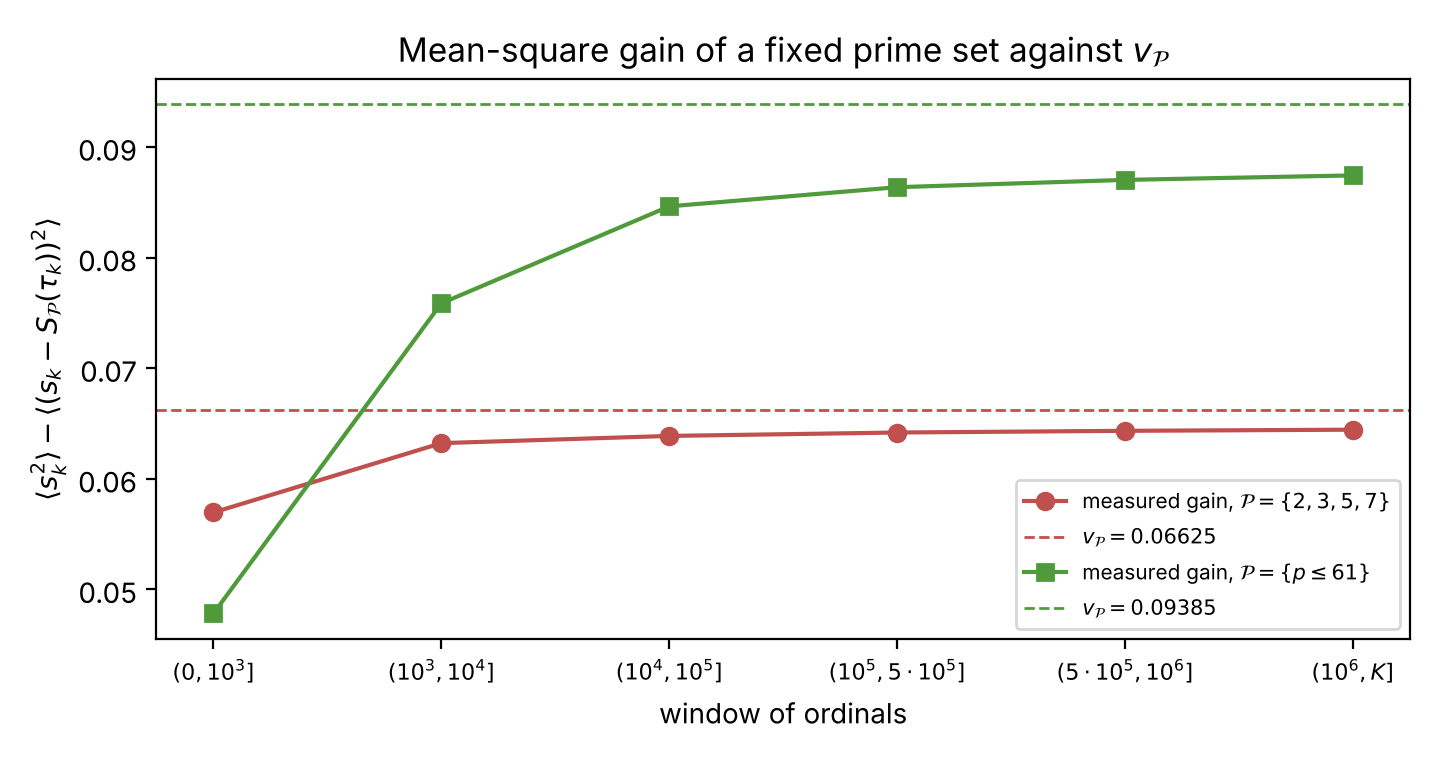
\includegraphics[width=0.86\textwidth]{fig06_gain_fixed_sets.png}
\caption{Mean-square gain $\langle s_k^2\rangle-\langle(s_k-S_\PP(\tau_k))^2\rangle$ of two fixed prime sets $\PP$ (full local factors) in each window of ordinals, and the constants $v_\PP$ (dashed) of Corollary~\CGref{cor:gain}.}
\label{fig:gain_fixed}
\end{figure}

\subsection{The response at the ordinates and its Fourier reduction}
\label{subsec:gamma_response}
Let $T,2T$ be non-ordinates, $p$ a prime, and
\begin{equation}
\mathcal A_{T,p}=-\frac{2\pi\sqrt p}{\#\IT}\int_T^{2T}G(t)\sin(t\log p)\lL(t)\,dt,
\qquad \mathcal S_{T,p}=\frac1T\int_T^{2T}S(t)^2p^{it}\,dt.
\label{eq:ATp_STp}
\end{equation}

\begin{proposition}[Unconditional separation of one- and two-point terms]\label{prop:gamma_response_exact}
\begin{equation}
\begin{split}
\Rg_p(\IT)={}&\mathcal A_{T,p}+\frac{\pi\sqrt p\,T\log p}{\#\IT}\Re\mathcal S_{T,p}-\frac{\pi\sqrt p}{\#\IT}\bigl[G^2\sin(t\log p)\bigr]_T^{2T}\\
&+\frac{\pi\sqrt p\log p}{\#\IT}\int_T^{2T}(G^2-S^2)\cos(t\log p)\,dt.
\end{split}
\label{eq:gamma_response_exact}
\end{equation}
If $\theta=\log p/L_T$ stays in a compact subset of $(0,1)$, the last two terms are $o(1)$ and
\begin{equation}
\Rg_p(\IT)=\mathcal A_{T,p}+2\pi^2\theta\sqrt p\,\bigl(1+O(1/L_T)\bigr)\Re\mathcal S_{T,p}+o(1).
\label{eq:gamma_response_scaled}
\end{equation}
\end{proposition}

\begin{proof}
Lemma~\CGref{lem:first_moment_identity} with $\psi(t)=\sin(t\log p)$ on $[T,2T]$, multiplied by $-2\pi\sqrt p/\#\IT$, gives \CGeqref{eq:gamma_response_exact}, because $\int_T^{2T}G^2\cos(t\log p)\,dt=T\Re\mathcal S_{T,p}+\int_T^{2T}(G^2-S^2)\cos(t\log p)\,dt$. On $[T,2T]$, $|G^2-S^2|\le2|S||\varpi|/\pi+\varpi^2/\pi^2\ll\log T/T$, so the last term is $O(\sqrt p\log p/T)$, and the boundary term is $O(\sqrt p\log^2T/(T\log T))$. Both are $o(1)$ for $p\le T^{\theta_1}$ with $\theta_1<1$. Finally $\#\IT=\frac{TL_T}{2\pi}(1+O(1/L_T))$.
\end{proof}

Let $f_T=S\mathbf1_{[T,2T]}$, let $\mathfrak m_T$ be its distributional derivative (a finite signed measure, since $f_T$ has compact support and bounded variation), and
\begin{equation}
\widehat{\mathfrak m}_T(\omega)=\int_\R e^{i\omega t}\,d\mathfrak m_T(t),\qquad \widehat{f_T}(\omega)=\int_\R f_T(t)e^{i\omega t}dt .
\label{eq:measure_def}
\end{equation}

\begin{theorem}[Unconditional shifted two-point representation]\label{thm:Fourier_exact}
For non-ordinates $T,2T$,
\begin{equation}
\widehat{\mathfrak m}_T(\omega)=\sum_{T<\gamma<2T}\nu(\gamma)e^{i\omega\gamma}-\int_T^{2T}\Bigl(\lL(t)+\frac{\varpi'(t)}\pi\Bigr)e^{i\omega t}\,dt+S(T)e^{i\omega T}-S(2T)e^{2i\omega T},
\label{eq:measure_expansion}
\end{equation}
$\widehat{\mathfrak m}_T(\omega)=-i\omega\widehat{f_T}(\omega)$, so that $\widehat{\mathfrak m}_T(0)=0$ and $\widehat{\mathfrak m}_T(\omega)/\omega$ extends continuously by $-i\widehat{f_T}$; and for every real $\omega_0$
\begin{equation}
\int_T^{2T}S(t)^2e^{i\omega_0t}\,dt=-\frac1{2\pi}\int_\R\frac{\widehat{\mathfrak m}_T(\omega)\widehat{\mathfrak m}_T(\omega_0-\omega)}{\omega(\omega_0-\omega)}\,d\omega,
\label{eq:Fourier_convolution}
\end{equation}
the integral converging absolutely.
\end{theorem}

\begin{proof}
On $(T,2T)$, $dS=dN-(\lL+\varpi'/\pi)dt$ as measures, with atoms $\nu(\gamma)\delta_\gamma$; the cutoff adds $S(T)\delta_T$ and $-S(2T)\delta_{2T}$. This gives $\mathfrak m_T$ and \CGeqref{eq:measure_expansion}. Since $f_T$ is of bounded variation with compact support, integration by parts gives $\int e^{i\omega t}d\mathfrak m_T=-i\omega\int f_Te^{i\omega t}dt$, the boundary terms vanishing. As $f_T\in L^1\cap L^2$ is real, Plancherel's identity applied to $f_T$ and $f_Te^{-i\omega_0t}$ gives $\int f_T^2e^{i\omega_0t}dt=\frac1{2\pi}\int\widehat{f_T}(\omega)\widehat{f_T}(\omega_0-\omega)\,d\omega$, absolutely convergent since $\int|\widehat{f_T}(\omega)\widehat{f_T}(\omega_0-\omega)|d\omega\le\|\widehat{f_T}\|_2^2=2\pi\|f_T\|_2^2$. Substitute $\widehat{f_T}=i\widehat{\mathfrak m}_T/\omega$.
\end{proof}

With $\omega_0=\theta L_T=\log p$ and $\omega=\alpha L_T$ put
\begin{equation}
\mathcal B_T(\theta)=\int_\R\frac{\widehat{\mathfrak m}_T(\alpha L_T)\widehat{\mathfrak m}_T((\theta-\alpha)L_T)}{\alpha(\theta-\alpha)}\,d\alpha,\qquad\text{so that}\qquad \mathcal S_{T,p}=-\frac{\mathcal B_T(\theta)}{2\pi TL_T}.
\label{eq:BT_scaled}
\end{equation}
Expanding the zero sums gives the weights $e^{i\alpha L_T\gamma}e^{i(\theta-\alpha)L_T\gamma'}=p^{i\gamma'}e^{i\alpha L_T(\gamma-\gamma')}$: $\mathcal S_{T,p}$ is a pair correlation of the zeros of the Riemann zeta function \emph{shifted by a prime frequency}, which a stationary pair correlation (a function of $\gamma-\gamma'$ only) does not determine.

\subsection{The kernel $\mathfrak K_\theta$}
\label{subsec:kernel}
For $0<\theta<1$ define the continuous, piecewise linear function
\begin{equation}
\mathfrak K_\theta(\alpha)=
\begin{cases}
\theta,&\alpha\le-1,\\
\theta-1-\alpha,&-1\le\alpha\le\theta-1,\\
0,&\theta-1\le\alpha\le1,\\
\alpha-1,&1\le\alpha\le1+\theta,\\
\theta,&\alpha\ge1+\theta,
\end{cases}
\label{eq:kernel_piecewise}
\end{equation}
equivalently, with $h(q)=\max(1-|q|,0)$,
\begin{equation}
\mathfrak K_\theta(\alpha)=1-h(\alpha)-h(\theta-\alpha)-h(\theta)+2\max\bigl(1-\max(|\alpha|,|\theta-\alpha|,\theta),0\bigr),
\label{eq:kernel_intersections}
\end{equation}
as one checks on each of the five intervals.

\begin{proposition}[Integral and support of the kernel]\label{prop:kernel_integral}
For $0<\theta<1$,
\begin{equation}
\int_\R\frac{\mathfrak K_\theta(\alpha)}{\alpha(\theta-\alpha)}\,d\alpha=-\frac{2\Phi(\theta)}{\theta},
\label{eq:kernel_integral}
\end{equation}
the integral being absolutely convergent, and $\mathfrak K_\theta(\alpha)=0$ whenever $|\alpha|+|\theta-\alpha|+\theta<2$.
\end{proposition}

\begin{proof}
$\mathfrak K_\theta$ is bounded and vanishes on $[\theta-1,1]$, which contains $0$ and $\theta$; the integrand is bounded, continuous outside $[\theta-1,1]$ and $O(\alpha^{-2})$ as $|\alpha|\to\infty$, hence absolutely integrable. It is invariant under $\alpha\mapsto\theta-\alpha$, which maps $[1,\infty)$ onto $(-\infty,\theta-1]$, so the integral is twice that over $[1,\infty)$. On $[1+\theta,\infty)$, $\frac{\theta}{\alpha(\theta-\alpha)}=\frac1\alpha-\frac1{\alpha-\theta}$, whose integral is $\lim_{y\to\infty}\bigl[\log\frac{\alpha}{\alpha-\theta}\bigr]_{1+\theta}^{y}=-\log(1+\theta)$. On $[1,1+\theta]$, $\frac{\alpha-1}{\alpha(\theta-\alpha)}=-\frac1{\theta\alpha}+\frac{\theta-1}{\theta(\theta-\alpha)}$, whose integral is $-\frac{\log(1+\theta)}\theta+\frac{\theta-1}\theta\log(1-\theta)$. The sum is $-\Phi(\theta)/\theta$; doubling gives \CGeqref{eq:kernel_integral}. If $\alpha>1$ then $|\alpha|+|\theta-\alpha|+\theta\ge\alpha+(\alpha-\theta)+\theta=2\alpha>2$, and if $\alpha<\theta-1$ the same follows by the symmetry; elsewhere $\mathfrak K_\theta=0$.
\end{proof}

\begin{proposition}[The square of the prime polynomial has no prime frequency]\label{prop:PY_square}
For $Y\ge2$, $T\ge2$ and every prime $p$, $\bigl|\frac1T\int_T^{2T}S^{\rm pr}_Y(t)^2p^{it}\,dt\bigr|\ll Y^3/T$, with an absolute constant. In particular, with $E_0=S-S^{\rm pr}_{Y_0}$, uniformly for primes $p\le T^{\theta_1}$ with fixed $\theta_1<1$,
\[
\mathcal S_{T,p}=\frac1T\int_T^{2T}\bigl(2S^{\rm pr}_{Y_0}(t)E_0(t)+E_0(t)^2\bigr)p^{it}\,dt+o(p^{-1/2}).
\]
\end{proposition}

\begin{proof}
Expanding the product of sines, $S^{\rm pr}_Y(t)^2p^{it}$ is a combination, with coefficients of modulus at most $\frac1{4\pi^2}(qr)^{-1/2}$, of $e^{i\lambda t}$ with $\lambda=\log(pq^{\pm1}r^{\pm1})$, $q,r<Y$ primes. No $\lambda$ vanishes: $p=qr$, $pq=r$, $pr=q$ and $pqr=1$ are impossible for primes. Write $e^\lambda=A/B$ with coprime positive integers; then $|\lambda|\ge\log(1+1/\min(A,B))\ge1/(2\min(A,B))$, and $\min(A,B)\le\max(r,qr)<Y^2$ in all cases, or $|\lambda|\ge\log8$. Hence $|\int_T^{2T}e^{i\lambda t}dt|\le2/|\lambda|\le4Y^2$, and the sum of the coefficients is $\ll(\sum_{q<Y}q^{-1/2})^2\ll Y$. For the second statement take $Y=Y_0=T^{1/160}$: $Y_0^3/T=T^{-157/160}=o(T^{-\theta_1/2})$.
\end{proof}

Thus the moving-prime law below is a statement about the terms that contain Selberg's remainder $E_0$. The bound $\int_T^{2T}E_0^4\ll T$ of Theorem~\CGref{thm:known_selberg_approx} gives only $|\frac1T\int E_0^2p^{it}|\ll1$ and $|\frac1T\int S^{\rm pr}_{Y_0}E_0p^{it}|\ll\sqrt{\log\log T}$, without the oscillation of size $p^{-1/2}$ that the law requires.

\subsection{The arithmetic of the Newton nonlinearity}
\label{subsec:newton_spectrum}
The corrected clocks of Section~\CGref{sec:iteration} are functions of the clock and of the phases $t\log q$ of the primes $q\le X_j$; the second step contains $S_{X_2}(x^{(1)}_k)$ with $x^{(1)}_k=\tau_k-S_{X_1}(\tau_k)/\lL(\tau_k)$, that is, compositions of prime phases. This subsection determines, without hypotheses, which frequencies such compositions can produce and which they cannot, and why the error of the corrected clocks in mean square and the response to a prime $p=T^\theta$ are different questions. Throughout, $M=\#\IT$.

\begin{proposition}[Spectral barrier at the clock points]\label{prop:spectral_barrier}
Let $0<\theta<1$, let $p=p(T)$ be a prime with $\log p/\log T\to\theta$, let $\epsilon_T\to0$, and let
\[
Q_T(t)=\sum_{a,b\le T^{\epsilon_T}}c_{a,b}\,e^{it\log(a/b)},\qquad\sum_{a,b}|c_{a,b}|\le T^{o(1)},
\]
with integers $a,b\ge1$ and complex coefficients. Then
\[
\frac{\sqrt p}{M}\sum_{k\in\IT}Q_T(\tau_k)\,p^{\,i\tau_k}=o(1).
\]
\end{proposition}

\begin{proof}
For each pair $(a,b)$ let $\Omega(x)=\tau_x\log(pa/b)/2\pi$; by \CGeqref{eq:clock}, $\Omega'(x)=\log(pa/b)/\log(\tau_x/2\pi)$ is continuous and monotone on the window, and since $|\log(a/b)|\le\epsilon_T\log T$, $\Omega'(x)=\theta+o(1)$ uniformly in $(a,b)$ and $x$. For $T\ge T_0$ therefore $\|\Omega'\|\ge\frac12\min(\theta,1-\theta)$ and Theorem~\CGref{thm:known_KL} gives $\sum_{k\in\IT}e^{i\tau_k\log(pa/b)}=O_\theta(1)$. Summing with the coefficients, $|\sum_kQ_T(\tau_k)p^{i\tau_k}|\ll_\theta T^{o(1)}$, and $\sqrt p/M=T^{\theta/2-1+o(1)}$.
\end{proof}

A combination of prime frequencies of multiplicative complexity $T^{o(1)}$ cannot respond, at the clock points, to a prime of scale $T^\theta$: the frequencies $\log(a/b)$ that could resonate with $\log p$ have $a$ or $b$ of size $T^{\theta+o(1)}$, which a polynomial in the phases of primes $\le T^{c}$ reaches only in degree $D\ge\min(\theta,1-\theta)/c$. For the first Newton step, $c=c_1$, this critical degree is $\asymp\min(\theta,1-\theta)\sqrt{\log\log T}$. The next lemma shows where the nonlinearity of the Newton step puts its spectral mass.

\begin{lemma}[Bessel expansion of a Newton phase]\label{lem:bessel}
Let $X\ge2$ and $\lambda\in\R$, and let $P_X=S^{(1)}_X$ be the prime part of $S_X$,
\[
P_X(t)=-\frac1\pi\sum_{q\le X}\frac{\sin(t\log q)}{\sqrt q}.
\]
With $z_q=\lambda/(\pi\sqrt q)$ and integer vectors $\mathbf j=(j_q)_{q\le X}$ indexed by the primes $q\le X$,
\begin{equation}
e^{-i\lambda P_X(t)}=\sum_{\mathbf j}A_{\mathbf j}\,e^{it\mathfrak l_{\mathbf j}},\qquad A_{\mathbf j}=\prod_{q\le X}J_{j_q}(z_q),\qquad\mathfrak l_{\mathbf j}=\sum_{q\le X}j_q\log q,
\label{eq:bessel_expansion}
\end{equation}
the series converging absolutely, $J_j$ the Bessel functions of integer order. Moreover
\begin{equation}
\sum_{\mathbf j}A_{\mathbf j}^2=1,\qquad\sum_{\mathbf j}A_{\mathbf j}^2\mathfrak l_{\mathbf j}=0,\qquad\sum_{\mathbf j}A_{\mathbf j}^2\mathfrak l_{\mathbf j}^2=\frac{\lambda^2}{2\pi^2}\sum_{q\le X}\frac{\log^2q}q,
\label{eq:bessel_moments}
\end{equation}
and, with $D(\mathbf j)=\sum_q|j_q|$ and $|z_q|\le1$ for all $q$, for every $s>0$ and $D\ge0$,
\begin{equation}
\sum_{D(\mathbf j)\ge D}A_{\mathbf j}^2\le e^{-sD}\exp\Bigl(\frac{C_s\lambda^2}{\pi^2}\sum_{q\le X}\frac1q\Bigr),\qquad C_s=e^{s}\exp(e^s/4+1/2).
\label{eq:bessel_tail}
\end{equation}
\end{lemma}

\begin{proof}
$e^{-i\lambda P_X(t)}=\prod_{q\le X}\exp(iz_q\sin(t\log q))$ and Jacobi's expansion $e^{iz\sin x}=\sum_{j\in\mathbb Z}J_j(z)e^{ijx}$ \cite[\S2.22]{Watson1944}, absolutely convergent since $|J_j(z)|\le(|z|/2)^{|j|}e^{z^2/4}/|j|!$ for real $z$ (from the power series of $J_j$); the product of finitely many absolutely convergent series is \CGeqref{eq:bessel_expansion}. Parseval's identity for $x\mapsto e^{iz\sin x}$ on $[0,2\pi]$ gives $\sum_jJ_j(z)^2=1$; for its derivative $iz\cos x\,e^{iz\sin x}$, whose Fourier coefficients are $ijJ_j(z)$, it gives $\sum_jj^2J_j(z)^2=\frac1{2\pi}\int_0^{2\pi}z^2\cos^2x\,dx=\frac{z^2}2$, and the inner product of the function with its derivative gives $\sum_jjJ_j(z)^2=\frac1{2\pi}\int_0^{2\pi}z\cos x\,dx=0$. Since $A_{\mathbf j}^2=\prod_qJ_{j_q}(z_q)^2$ and $\mathfrak l_{\mathbf j}$ is linear in $\mathbf j$, the three identities \CGeqref{eq:bessel_moments} follow by expanding the products. For \CGeqref{eq:bessel_tail}, $J_0(z)^2\le1$ and, for $|z|\le1$,
\[
\sum_{j\ne0}e^{s|j|}J_j(z)^2\le2e^{z^2/2}\sum_{j\ge1}\frac{(e^sz^2/4)^j}{(j!)^2}\le2e^{z^2/2}\cdot\frac{e^sz^2}4\exp\Bigl(\frac{e^sz^2}4\Bigr)\le C_sz^2,
\]
so $\sum_{\mathbf j}e^{sD(\mathbf j)}A_{\mathbf j}^2=\prod_q\sum_je^{s|j|}J_j(z_q)^2\le\prod_q(1+C_sz_q^2)\le\exp(C_s\sum_qz_q^2)$, and Chebyshev's inequality in $D$ gives \CGeqref{eq:bessel_tail}.
\end{proof}

\begin{proposition}[Spectral concentration and dispersion of the Newton phases]\label{prop:newton_spectrum}
Let $X_1=T^{c_1}$, $c_1=H_0^{-1/2}$, and for a prime power $n$ and $t>2\pi$ let $\lambda_n(t)=\log n/\lL(t)$, so that $\sin(x^{(1)}_k\log n)=\Im\bigl(e^{i\tau_k\log n}e^{-i\lambda_n(\tau_k)S_{X_1}(\tau_k)}\bigr)$; the prime-power part $S_{X_1}-P_{X_1}$ contributes to $e^{-i\lambda S_{X_1}}$ a further factor of the form \CGeqref{eq:bessel_expansion}, with $z_{p^m}=\lambda/(\pi mp^{m/2})$ at the frequencies $m\log p$, which changes nothing below and is omitted.
\begin{enumerate}[label=(\alph*),leftmargin=2em]
\item (First step: concentration in low degrees.) For $n\le X_1$ and $t\in[T,2T]$, $|\lambda_n(t)|\le2\pi c_1(1+o(1))$, and in \CGeqref{eq:bessel_tail} with $X=X_1$, $\lambda=\lambda_n(t)$, the exponent $\frac{C_s\lambda^2}{\pi^2}\sum_{q\le X_1}\frac1q\le4C_sc_1^2H_0(1+o(1))\le5C_s$ is bounded: the mass of $e^{-i\lambda_n P_{X_1}}$ in degrees $\ge D$ is $\le C'_se^{-sD}$, uniformly in $n\le X_1$ and $t$.
\item (Second step: dispersion.) For $n\le X_2=T^{c_2}$, $c_2=H_1^{-1/2}$, the mass in degrees $\ge D$ is only bounded by $e^{-sD}\exp(C''_sH_0/H_1)$, which is not uniform, but the frequencies $\mathfrak l_{\mathbf j}$ of $e^{-i\lambda_n(t)P_{X_1}}$ have, by \CGeqref{eq:bessel_moments} and Theorem~\CGref{thm:known_mertens},
\[
\Bigl(\sum_{\mathbf j}A_{\mathbf j}^2\mathfrak l_{\mathbf j}^2\Bigr)^{1/2}=\frac{|\lambda_n(t)|}{2\pi}\log X_1\,(1+o(1))\le c_1c_2\log T\,(1+o(1)),
\]
hence, for every $0<\theta<1$,
\begin{equation}
\sum_{|\mathfrak l_{\mathbf j}|\ge\theta\log T}A_{\mathbf j}^2\le\frac{c_1^2c_2^2}{\theta^2}(1+o(1))=\frac{1+o(1)}{\theta^2H_0H_1}.
\label{eq:newton_dispersion}
\end{equation}
\end{enumerate}
\end{proposition}

\begin{proof}
(a) $\lambda_n(t)=\log n/\lL(t)\le c_1\log T/\lL(T)=2\pi c_1(1+O(1/\log T))$ and $\sum_{q\le X_1}1/q=\log\log X_1+O(1)\le H_0$; $|z_q|\le|\lambda|/\pi\le1$. (b) The same with $c_2$, $\sum_{q\le X_1}\log^2q/q=\frac12\log^2X_1(1+o(1))$ by partial summation from Theorem~\CGref{thm:known_mertens}, and Chebyshev's inequality for the probability measure $A_{\mathbf j}^2$ on the vectors $\mathbf j$.
\end{proof}

The second Newton step therefore generates frequencies of arbitrarily high multiplicative degree, but its spectral mass at the frequencies $|\mathfrak l_{\mathbf j}|\ge\theta\log T$ of the moving primes $p=T^\theta$ is $\ll(H_0H_1)^{-1}$: the reduction of the mean-square error (Theorem~\CGref{thm:uniform_iteration}) and the reconstruction of the response $1-\Phi(\theta)$ at $p=T^\theta$ are different objectives, the second living in a spectral tail that the first does not see. For a fixed cutoff the compositions produce no exact resonance either.

\begin{proposition}[Exact orthogonality for a fixed cutoff]\label{prop:orthogonality}
Let $X\ge2$ be fixed, let $\mathfrak F$ be a continuous function on the torus $\mathbb T^{\#\{q\le X\}}$, and let $\mathfrak F_X(t)=\mathfrak F\bigl((t\log q)_{q\le X}\bigr)$. Then for every prime $p>X$,
\[
\lim_{U\to\infty}\frac1U\int_U^{2U}e^{it\log p}\mathfrak F_X(t)\,dt=0 .
\]
\end{proposition}

\begin{proof}
Given $\varepsilon>0$, choose a trigonometric polynomial $\mathfrak P(\mathbf y)=\sum_{\mathbf m}d_{\mathbf m}e^{i\mathbf m\cdot\mathbf y}$ on the torus with $\sup|\mathfrak F-\mathfrak P|\le\varepsilon$ (Stone--Weierstrass). Then $e^{it\log p}\mathfrak P((t\log q)_q)=\sum_{\mathbf m}d_{\mathbf m}e^{it\log(p\prod_qq^{m_q})}$, and each frequency $\log(p\prod_qq^{m_q})$ is nonzero, by unique factorization ($p$ does not occur among the $q$); so each term has mean $O_{\mathbf m}(1/U)$ over $[U,2U]$, and the limit superior of the modulus of the mean of $e^{it\log p}\mathfrak F_X$ is at most $\varepsilon$.
\end{proof}

What a corrected clock with growing cutoff can create is not an exact resonance but frequencies near $\log p$ in finite windows, through the degrees above the critical one; their uniform control is what a proof of the moving-prime law at the corrected clock points would need, and it is not given here. The estimate that would connect the two problems is
\begin{equation}
\sup_{T^a\le p\le T^b}\sqrt p\,\Bigl|\frac1M\sum_{k\in\IT}\lL(\tau_k)\bigl(x^{(m)}_k-\gamma_k\bigr)e^{i\tau_k\log p}\Bigr|\longrightarrow0\qquad(0<a<b<1),
\label{eq:transfer_estimate}
\end{equation}
for some $m\le m^*$: it would transfer the response at the ordinates to the response at the $m$-th corrected clock, which is a function of the clock and the primes alone. Nothing of the kind is proved for a single prime; Theorem~\CGref{thm:uniform_iteration} together with Proposition~\CGref{prop:spectral_energy}(c) controls the left side only in $L^2(dp/p)$, with total error $O(1)$.

\subsubsection*{The computable part of the response}
For the corrected clocks of Section~\CGref{sec:iteration}, the response $\Rt_p$ splits exactly into a part computable from the clock and the primes and a part carried by the error. Write, for $m\ge1$ and a prime $p$,
\begin{equation}
\begin{split}
\mathcal A^{(m)}_p&=-2\pi\sqrt p\bigl\langle\lL(\tau_k)(\tau_k-x^{(m)}_k)\sin(\tau_k\log p)\bigr\rangle_{\IT},\\
\mathcal E^{(m)}_p&=-2\pi\sqrt p\bigl\langle\lL(\tau_k)(x^{(m)}_k-\gamma_k)\sin(\tau_k\log p)\bigr\rangle_{\IT},\\
\mathcal D^{(m)}_p&=-2\pi\sqrt p\bigl\langle S_{X_m}(\tau_k)\sin(\tau_k\log p)\bigr\rangle_{\IT},\\
\mathcal B^{(m)}_p&=-2\pi\sqrt p\bigl\langle B^{(m)}_k\sin(\tau_k\log p)\bigr\rangle_{\IT},\qquad B^{(m)}_k=S_{X_m}(x^{(m-1)}_k)-S_{X_m}(\tau_k),
\end{split}
\label{eq:computable_parts}
\end{equation}
so that $\mathcal A^{(m)}$ is the response of the correction applied by the $m$ steps, $\mathcal D^{(m)}$ that of the prime polynomial evaluated on the clock, $\mathcal B^{(m)}$ that of its transport to the previous points, and $\mathcal E^{(m)}$ that of the residual error.

\begin{theorem}[Computable and residual responses]\label{thm:computable_response}
Let $X_m=T^{c_m}$ with $c_m\le\frac12$ and $x^{(m)}_k$ as in \CGeqref{eq:newton_iteration}. Then:
\begin{enumerate}[label=(\roman*),leftmargin=2em]
\item $\Rt_p(\IT)=\mathcal A^{(m)}_p+\mathcal E^{(m)}_p+O(\sqrt p/T)$ and $\mathcal A^{(m)}_p=\mathcal D^{(m)}_p+\mathcal B^{(m)}_p+O(\sqrt p\,T^{c_m-1})$, for every $m\ge1$ and every prime $p$; $\mathcal B^{(1)}_p=0$.
\item For $\varepsilon>0$, uniformly for primes $p$ with $pX_m\le T^{1-\varepsilon}$,
\begin{equation}
\mathcal D^{(m)}_p=\mathbf 1_{[p\le X_m]}+O_\varepsilon\Bigl(\frac{(p+X_m)\log T}{T}\Bigr).
\label{eq:diagonal_response}
\end{equation}
\item Hence $\mathcal A^{(1)}_p=\mathbf 1_{[p\le X_1]}+o(1)$ for $pX_1\le T^{1-\varepsilon}$: the first step has no response at the moving primes $p=T^\theta$, $0<\theta<1$. For every $m$ and $X_m<p$, $pX_m\le T^{1-\varepsilon}$,
\begin{equation}
\Rt_p(\IT)=\mathcal B^{(m)}_p+\mathcal E^{(m)}_p+o(1):
\label{eq:moving_response_split}
\end{equation}
the response of the ordinates to a moving prime is the response of the transport plus that of the residual.
\item For $0<b<1$, $\sum_{p\le T^b}|\mathcal B^{(m)}_p|^2/p\le2\pi^2(1+o_b(1))\langle(B^{(m)}_k)^2\rangle_{\IT}$, and $\langle(B^{(2)}_k)^2\rangle\ll H_0/H_1$.
\end{enumerate}
\end{theorem}

\begin{proof}
(i) $s_k=\lL(\tau_k)\delta_k-\chi_k=\lL(\tau_k)(\tau_k-x^{(m)}_k)+\lL(\tau_k)(x^{(m)}_k-\gamma_k)-\chi_k$ with $0\le\chi_k\le1/T$, and $\lL(\tau_k)(\tau_k-x^{(m)}_k)=S_{X_m}(x^{(m-1)}_k)+R_{m,k}$ with $|R_{m,k}|\ll T^{c_m-1}$ (Lemma~\CGref{lem:second_identity}); $S_{X_m}(x^{(m-1)}_k)=S_{X_m}(\tau_k)+B^{(m)}_k$.

(ii) $S_{X_m}(\tau_k)\sin(\tau_k\log p)=\sum_{n\in A_{X_m}}a_n\bigl[\tfrac12\cos(\tau_k\log\tfrac np)-\tfrac12\cos(\tau_k\log np)\bigr]$. The term $n=p$ exists exactly when $p\le X_m$ and equals $\frac{a_p}2(1-\cos(2\tau_k\log p))$; since $-2\pi\sqrt p\cdot\frac{a_p}2=1$, it contributes $1-\langle\cos(2\tau_k\log p)\rangle$. Every other frequency $\omega\in\{\log(n/p),\log(np),2\log p\}$ satisfies $|\omega|\le\log(X_mp)\le(1-\varepsilon)\log T$, so $\Omega(x)=\tau_x|\omega|/2\pi$ has $\Omega'\le1-\varepsilon$ and $\|\Omega'\|\ge\min(|\omega|/\log T,\varepsilon)$ on the window; Theorem~\CGref{thm:known_KL} gives $|\langle e^{i\tau_k\omega}\rangle_{\IT}|\ll_\varepsilon\frac1{T|\omega|}+\frac1{T\log T}$. For $|\log(n/p)|$: if $n\notin[p/2,2p]$ then $|\omega|\ge\log2$; if $n\in[p/2,2p]$, $n\ne p$, then $|\omega|\ge|n-p|/(2p)$ and $\sum_{n\in[p/2,2p]}|a_n|/|\omega|\ll p^{-1/2}\sum_{0<|n-p|\le p}p/|n-p|\ll\sqrt p\log p$. Summing with $\sum_{A_{X_m}}|a_n|\ll\sqrt{X_m}$ and multiplying by $2\pi\sqrt p$ gives \CGeqref{eq:diagonal_response}.

(iii) is (i) and (ii). (iv) is Proposition~\CGref{prop:spectral_energy} with $r_k=B^{(m)}_k$; for $m=2$, $|B^{(2)}_k|\le2|y_k|g_2(\tau_k)$ with $y_k=\tau_k-x^{(1)}_k$ and $g_2=\mathcal M(\varphi S'_{X_2})$ (as in Proposition~\CGref{prop:deformation}), and the sampling of $g_2$ at the clock points in $L^8$ (proof of Theorem~\CGref{thm:second_step}) and $\langle y_k^8\rangle\ll H_0^4/\log^8T$ give $\langle(B^{(2)})^2\rangle\le4\langle y^4\rangle^{1/2}\langle g_2(\tau)^4\rangle^{1/2}\ll\frac{H_0}{\log^2T}(c_2\log T)^2=H_0/H_1$.
\end{proof}

By \CGeqref{eq:moving_response_split}, a limit of $\Rt_p$ at $p=T^\theta$ is a statement about $\mathcal B^{(m)}_p+\mathcal E^{(m)}_p$. For the transport, the Bessel expansion of Lemma~\CGref{lem:bessel} gives every frequency of degree below the critical one as a non-resonant mean $O(T^{-\varepsilon})$, but their number has $\ell^1$ mass $\exp(c\,c_2\sqrt{X_1}/\log X_1)$ while only the $\ell^2$ mass is bounded; and the factor $\sqrt p$ in \CGeqref{eq:computable_parts} makes any $\ell^2$ or energy bound useless for a single prime. Whether $\mathcal B^{(m)}_p\to0$ (the response of the moving primes then living entirely in the residual) or $\mathcal B^{(m)}_p$ tends to an arithmetic function of $\theta$ is not decided by the estimates of this paper.

\emph{Computation.} Table~\CGref{tab:computable_response} lists $\Rt_p$, $\mathcal D^{(m)}_p$, $\mathcal B^{(m)}_p$ and $\mathcal E^{(m)}_p$ at $T=2^{19}$ for the cutoff sets of Table~\CGref{tab:iteration} and for primes from $\theta=0.10$ to $\theta=1.04$ (\texttt{opc\_computable\_response\_v14.py}). At this height the stationary band of the clock is $83\,443\lesssim n\lesssim166\,886$, so \CGeqref{eq:diagonal_response} applies only when $pX_m<83\,443$; where $pX_m$ enters the band, $\mathcal D^{(m)}_p$ and $\mathcal B^{(m)}_p$ take values of order one through the pair resonance of Proposition~\CGref{prop:pair_resonance} (for instance $\mathcal D^{(3)}_{1009}=0.207$ with $X_3=724$, $\mathcal D^{(1)}_{50021}=1.199$ with $X_1=3$), which is a finite-height effect and not a response at $\theta$. In the clean range $X_m<p$, $pX_m<83\,443$, the computable response is small: $|\mathcal B^{(2)}_p|\le0.07$ and $|\mathcal B^{(3)}_p|\le0.08$ at $p=101$ and $211$, against $\Rt_p=0.84$ and $0.79$, and the residual carries the rest. This is descriptive, at one height, and consistent with $\mathcal B^{(m)}_p\to0$ for fixed $m$; it says nothing about $m=m^*(T)$.

\begin{table}[htbp]
\centering\footnotesize
\caption{Computable and residual responses at $T=2^{19}$ ($\#\IT=977\,804$) for the three cutoff sets of Table~\CGref{tab:iteration}: $\Rt_p$ and, for $m=1,2,3$, the diagonal part $\mathcal D^{(m)}_p$, the transport part $\mathcal B^{(m)}_p$ and the residual $\mathcal E^{(m)}_p$ of \CGeqref{eq:computable_parts}. A dagger marks $pX_m\ge83\,443$ (pair resonance); prime powers $n=q^j$ with $q\le X_m$ and the width of the stationary band blur this boundary, e.g.\ $\mathcal D^{(1)}_{10007}=0.090$ with $X_1=3$ comes from $n=8$, $8p=80\,056$. Values from \texttt{outputs/table\_L\_computable\_response.csv}.}
\label{tab:computable_response}
\setlength{\tabcolsep}{3pt}
\begin{tabular}{rr r rrr rrr rrr}
\toprule
$p$ & $\theta$ & $\Rt_p$ & $\mathcal D^{(1)}$ & $\mathcal B^{(1)}$ & $\mathcal E^{(1)}$ & $\mathcal D^{(2)}$ & $\mathcal B^{(2)}$ & $\mathcal E^{(2)}$ & $\mathcal D^{(3)}$ & $\mathcal B^{(3)}$ & $\mathcal E^{(3)}$\\
\midrule
\multicolumn{12}{l}{$(c_1,c_2,c_3)=(\frac1{10},\frac15,\frac13)$, $X=(3,13,80)$}\\
3 & 0.097 & 0.974 & 1.000 & 0 & $-0.026$ & 1.000 & $-0.033$ & 0.007 & 1.000 & $-0.026$ & $-0.001$\\
7 & 0.172 & 0.957 & 0.000 & 0 & 0.957 & 1.000 & $-0.026$ & $-0.017$ & 1.000 & $-0.084$ & 0.041\\
31 & 0.303 & 0.900 & 0.000 & 0 & 0.900 & 0.000 & 0.001 & 0.898 & 1.001 & $-0.097$ & $-0.005$\\
101 & 0.407 & 0.835 & 0.000 & 0 & 0.835 & 0.001 & 0.003 & 0.831 & 0.002 & 0.047 & 0.785\\
211 & 0.472 & 0.791 & 0.001 & 0 & 0.790 & 0.001 & 0.006 & 0.784 & 0.003 & 0.079 & 0.709\\
1009 & 0.610 & 0.703 & 0.002 & 0 & 0.701 & 0.012 & 0.019 & 0.672 & 0.012 & 0.186 & 0.504\\
2003 & 0.671 & 0.678 & 0.010 & 0 & 0.668 & 0.022 & 0.038 & 0.618 & 0.238$^\dagger$ & 0.147 & 0.293\\
10007 & 0.813 & 0.626 & 0.090 & 0 & 0.536 & 0.330$^\dagger$ & 0.090 & 0.206 & 0.332$^\dagger$ & 0.246 & 0.048\\
50021 & 0.955 & 1.238 & 1.199$^\dagger$ & 0 & 0.039 & 1.199$^\dagger$ & 0.035 & 0.004 & 1.199$^\dagger$ & 0.077 & $-0.038$\\
100003 & 1.016 & 0.026 & 0.000 & 0 & 0.026 & 0.001 & 0.030 & $-0.005$ & 0.001 & 0.003 & 0.021\\
\multicolumn{12}{l}{$(c_1,c_2,c_3)=(\frac15,\frac13,\frac12)$, $X=(13,80,724)$}\\
3 & 0.097 & 0.974 & 1.000 & 0 & $-0.026$ & 1.000 & $-0.067$ & 0.041 & 1.000 & $-0.002$ & $-0.024$\\
31 & 0.303 & 0.900 & 0.000 & 0 & 0.900 & 1.001 & $-0.105$ & 0.004 & 1.001 & $-0.077$ & $-0.024$\\
101 & 0.407 & 0.835 & 0.001 & 0 & 0.834 & 0.002 & 0.035 & 0.797 & 1.002 & 0.044 & $-0.212$\\
211 & 0.472 & 0.791 & 0.001 & 0 & 0.790 & 0.003 & 0.065 & 0.723 & 1.131$^\dagger$ & $-0.063$ & $-0.277$\\
1009 & 0.610 & 0.703 & 0.012 & 0 & 0.691 & 0.012 & 0.170 & 0.521 & 0.207$^\dagger$ & 0.347 & 0.149\\
2003 & 0.671 & 0.678 & 0.022 & 0 & 0.656 & 0.238$^\dagger$ & 0.131 & 0.309 & 0.264$^\dagger$ & 0.311 & 0.103\\
10007 & 0.813 & 0.626 & 0.330$^\dagger$ & 0 & 0.296 & 0.332$^\dagger$ & 0.254 & 0.039 & 0.332$^\dagger$ & 0.249 & 0.045\\
\multicolumn{12}{l}{$(c_1,c_2,c_3)=(\frac13,\frac12,\frac12)$, $X=(80,724,724)$}\\
3 & 0.097 & 0.974 & 1.000 & 0 & $-0.026$ & 1.000 & $-0.096$ & 0.069 & 1.000 & 0.028 & $-0.055$\\
31 & 0.303 & 0.900 & 1.001 & 0 & $-0.102$ & 1.001 & $-0.122$ & 0.020 & 1.001 & $-0.040$ & $-0.062$\\
101 & 0.407 & 0.835 & 0.002 & 0 & 0.832 & 1.002 & $-0.008$ & $-0.160$ & 1.002 & $-0.283$ & 0.115\\
211 & 0.472 & 0.791 & 0.003 & 0 & 0.788 & 1.131$^\dagger$ & $-0.114$ & $-0.226$ & 1.131$^\dagger$ & $-0.416$ & 0.076\\
1009 & 0.610 & 0.703 & 0.012 & 0 & 0.691 & 0.207$^\dagger$ & 0.350 & 0.146 & 0.207$^\dagger$ & 0.174 & 0.322\\
2003 & 0.671 & 0.678 & 0.238$^\dagger$ & 0 & 0.440 & 0.264$^\dagger$ & 0.320 & 0.094 & 0.264$^\dagger$ & 0.174 & 0.240\\
\bottomrule
\end{tabular}
\end{table}

\subsection{The moving-prime law under Hypotheses U and W}
\label{subsec:conditional_law}

\begin{hypothesis}[Hypothesis U: uniform one-particle input]\label{hyp:uniform_prime}
For every $0<\theta_0<\theta_1<1$, uniformly for primes with $\theta_0\le\log p/L_T\le\theta_1$, $\mathcal A_{T,p}=1+o(1)$.
\end{hypothesis}
A sufficient condition is the uniform estimate $\sup_{T\le t\le2T}|\sum_{T<\gamma_k\le t}p^{i\gamma_k}+\frac{(t-T)\log p}{2\pi\sqrt p}|=o(T\log p/\sqrt p)$ in that range, by two integrations by parts as in the proof of Theorem~\CGref{thm:projection}. Theorem~\CGref{thm:landau_line} gives it only for $p\le T^{o(1)}$, through the error term $t\log^2p/\log t$.

\begin{hypothesis}[Hypothesis W: weighted arithmetic bridge]\label{hyp:weighted_bridge}
Uniformly for primes with $\theta$ in any compact subset of $(0,1)$,
\begin{equation}
\int_\R\frac{\widehat{\mathfrak m}_T(\alpha L_T)\widehat{\mathfrak m}_T((\theta-\alpha)L_T)+\mathcal N_Tp^{-1/2}\mathfrak K_\theta(\alpha)}{\alpha(\theta-\alpha)}\,d\alpha=o\Bigl(\frac{TL_T}{\sqrt p}\Bigr),
\label{eq:weighted_arithmetic_bridge}
\end{equation}
with the continuous extensions of $\widehat{\mathfrak m}_T(\omega)/\omega$ at $\omega=0$.
\end{hypothesis}

\begin{proposition}[Moving-prime law under Hypotheses U and W]\label{prop:conditional_universal}
Under Hypothesis~W,
\begin{equation}
\mathcal S_{T,p}=-\frac{1}{2\pi^2\sqrt p}\frac{\Phi(\theta)}{\theta}+o(p^{-1/2}).
\label{eq:CTp_target}
\end{equation}
Under Hypotheses~U and W, or U and the real part of \CGeqref{eq:CTp_target}, uniformly for $\theta$ in compact subsets of $(0,1)$,
\begin{equation}
\Rg_p(\IT)=1-\Phi(\theta)+o(1).
\label{eq:conditional_universal}
\end{equation}
Conversely, under Hypothesis~U, \CGeqref{eq:conditional_universal} is equivalent to the real part of \CGeqref{eq:CTp_target}. Nothing is asserted about $\Rt_p$.
\end{proposition}

\begin{proof}
The integral of the kernel term in \CGeqref{eq:weighted_arithmetic_bridge} converges absolutely (Proposition~\CGref{prop:kernel_integral}); hence so does that of the first term, which is $\mathcal B_T(\theta)$, and by \CGeqref{eq:kernel_integral} $\mathcal B_T(\theta)=\frac{\mathcal N_T}{\sqrt p}\frac{2\Phi(\theta)}\theta+o(TL_T/\sqrt p)=\frac{TL_T}{\pi\sqrt p}\frac{\Phi(\theta)}\theta+o(TL_T/\sqrt p)$; \CGeqref{eq:BT_scaled} gives \CGeqref{eq:CTp_target}. Then $\sqrt p\,\Re\mathcal S_{T,p}=O(1)$, so in \CGeqref{eq:gamma_response_scaled} the factor $1+O(1/L_T)$ contributes $o(1)$ and $2\pi^2\theta\sqrt p\,\Re\mathcal S_{T,p}=-\Phi(\theta)+o(1)$; with $\mathcal A_{T,p}=1+o(1)$ this is \CGeqref{eq:conditional_universal}. Conversely, solve \CGeqref{eq:gamma_response_scaled} for $\Re\mathcal S_{T,p}$.
\end{proof}

\begin{remark}\label{rem:scale_gap}
$\Phi(\theta)=2\sum_{j\ge1}\frac{\theta^{2j}}{(2j-1)2j}=\theta^2+\frac{\theta^4}6+\frac{\theta^6}{15}+\cdots$, so $1-\theta^2$ is only the quadratic truncation of \CGeqref{eq:conditional_universal}, and $1-\Phi(\theta)$ vanishes at $\theta=0.9036\ldots$. Hypotheses U and W are not consequences of Theorem~\CGref{thm:landau_line}, which reaches only $\theta\to0$. By Proposition~\CGref{prop:PY_square}, \CGeqref{eq:CTp_target} is a statement about $\frac1T\int(2S^{\rm pr}_{Y_0}E_0+E_0^2)p^{it}$, with required error $o(p^{-1/2})=T^{-\theta/2+o(1)}$.
\end{remark}

%======================================================================
\section{Heuristic support and numerical evidence}
\label{sec:heuristic}

\emph{This section contains no statement about the Riemann zeta function that is used elsewhere. Subsection~\CGref{subsec:det_model} proves a theorem about a random-matrix model; its relevance to the zeros of the Riemann zeta function is a heuristic.}

\subsection{A determinantal model whose connected kernel is $\mathfrak K_\theta$}
\label{subsec:det_model}
On a circle of length $R_0$ let $\Pi_{\mathfrak n}$ be the orthogonal projection onto $\mathfrak n$ consecutive Fourier modes, and consider its determinantal point process, which has exactly $\mathfrak n$ points. For $q\in R_0^{-1}\mathbb Z$ let $\Xi_q$ be the centred linear statistic of $y\mapsto e^{2\pi iqy}$, so that $\Xi_0=0$ and $\overline{\Xi_q}=\Xi_{-q}$. Let $R_0,\mathfrak n\to\infty$ with $\mathfrak n/R_0\to1$, so that the local kernel tends to the sine kernel. For lattice $\theta>0$ and real $\iota_1,\iota_2$ the tilt
\begin{equation}
d\mathbb P_{\iota_1,\iota_2}=\frac{\exp\{-\iota_1\Re\Xi_{-\theta}-\iota_2\Im\Xi_{-\theta}\}}{\mathbb E\exp\{-\iota_1\Re\Xi_{-\theta}-\iota_2\Im\Xi_{-\theta}\}}\,d\mathbb P_{0,0}
\label{eq:real_tilt}
\end{equation}
is a probability measure (the statistics are bounded), and differentiation at $(0,0)$, justified by boundedness, gives $(\partial_{\iota_1}+i\partial_{\iota_2})\operatorname{Cov}_{\iota_1,\iota_2}(\Xi_\alpha,\Xi_{\theta-\alpha})|_{(0,0)}=-\operatorname{cum}_3(\Xi_\alpha,\Xi_{\theta-\alpha},\Xi_{-\theta})$, the third joint cumulant.

\begin{theorem}[Connected kernel of the model]\label{thm:sine_kernel}
Let lattice frequencies tend to $\alpha,\theta-\alpha,-\theta$ with $0<\theta<1$. Then $R_0^{-1}\operatorname{cum}_3(\Xi_\alpha,\Xi_{\theta-\alpha},\Xi_{-\theta})\to\mathfrak K_\theta(\alpha)$ and $R_0^{-1}\operatorname{cum}_2(\Xi_\theta,\Xi_{-\theta})\to\theta$.
\end{theorem}

\begin{proof}
For commuting multiplication operators $\mathsf m_1,\mathsf m_2,\mathsf m_3$, the third joint cumulant of the corresponding linear statistics of a determinantal process with projection kernel is \cite{Soshnikov2002}
\begin{equation}
\begin{split}
\operatorname{cum}_3={}&\operatorname{Tr}(\mathsf m_1\mathsf m_2\mathsf m_3\Pi_{\mathfrak n})-\operatorname{Tr}(\mathsf m_1\mathsf m_2\Pi_{\mathfrak n}\mathsf m_3\Pi_{\mathfrak n})-\operatorname{Tr}(\mathsf m_1\mathsf m_3\Pi_{\mathfrak n}\mathsf m_2\Pi_{\mathfrak n})-\operatorname{Tr}(\mathsf m_2\mathsf m_3\Pi_{\mathfrak n}\mathsf m_1\Pi_{\mathfrak n})\\
&+\operatorname{Tr}(\mathsf m_1\Pi_{\mathfrak n}\mathsf m_2\Pi_{\mathfrak n}\mathsf m_3\Pi_{\mathfrak n})+\operatorname{Tr}(\mathsf m_1\Pi_{\mathfrak n}\mathsf m_3\Pi_{\mathfrak n}\mathsf m_2\Pi_{\mathfrak n}),
\end{split}
\label{eq:third_cumulant_trace}
\end{equation}
the third-order term of the expansion of $\log\det(\mathrm{Id}+\Pi_{\mathfrak n}(e^{\mathsf m}-1)\Pi_{\mathfrak n})$. Multiplication by $e^{2\pi iqy}$ shifts a mode by $R_0q$; a trace with two projections counts the overlap of two integer intervals of length $\mathfrak n$, and a trace with three their triple overlap. For the shifts $R_0\alpha$, $R_0(\theta-\alpha)$, $-R_0\theta$, whose sum is $0$, the triple overlap has length $\max(\mathfrak n-R_0\max(|\alpha|,|\theta-\alpha|,\theta),0)$ for both cyclic orders, and the pair overlaps have lengths $R_0h(\cdot)+o(R_0)$. Dividing by $R_0$ gives the right side of \CGeqref{eq:kernel_intersections}. The same count for two operators gives $R_0^{-1}\operatorname{cum}_2(\Xi_\theta,\Xi_{-\theta})\to1-h(\theta)=\theta$.
\end{proof}

\emph{Why Hypothesis~W is plausible.} A window $[T,2T]$ contains about $\mathcal N_T=TL_T/2\pi$ zeros of the Riemann zeta function at unit mean spacing after unfolding, and the one-particle prime amplitude in Hypothesis~U is $-\mathcal N_T\theta/\sqrt p$. This equals the linear response of $\mathbb E\,\Xi_\theta$ to the tilt \CGeqref{eq:real_tilt} with $\iota_1=2/\sqrt p$, $\iota_2=0$ and $R_0=\mathcal N_T$, namely $-\frac{\iota_1}2\operatorname{cum}_2(\Xi_\theta,\Xi_{-\theta})\sim-\mathcal N_T\theta/\sqrt p$, by the susceptibility $\theta$ of Theorem~\CGref{thm:sine_kernel}. If the zeros responded to the prime $p$ like the model, the connected product in \CGeqref{eq:BT_scaled} would be $-\mathcal N_T\mathfrak K_\theta(\alpha)/\sqrt p$, which is the content of Hypothesis~W. This is an analogy, not an argument: stationary sine-kernel statistics do not determine the shifted correlation \CGeqref{eq:BT_scaled}, and convergence on compact sets would not control the singular weight and the tails. Note that $\mathfrak K_\theta$ vanishes where $|\alpha|+|\theta-\alpha|+\theta<2$ (Proposition~\CGref{prop:kernel_integral}), so the whole value $-2\Phi(\theta)/\theta$ comes from frequencies outside that region.

\subsection{Numerical evidence}
\label{subsec:numerics_law}

\begin{conjecture}\label{conj:law}
For primes with $\theta=\log p/L_T$ in compact subsets of $(0,1)$, $\Rg_p(\IT)=1-\Phi(\theta)+o(1)$.
\end{conjecture}

For all $2262$ primes $p\le20\,000$ we compute $\Rg_p$ and $\Rt_p$ on the five windows of ordinals above $k=1000$, with $\theta=\log p/\operatorname{median}_k\log(\tau_k/2\pi)$, and compare the primes with $0<\theta<1$ with $1-\Phi(\theta)$. Table~\CGref{tab:response_errors} separates individual errors from bin means over $\theta$-bins of width $0.05$ containing at least five primes; Table~\CGref{tab:response_bins} lists the bins of the two top windows, and Figure~\CGref{fig:response_law} all bins.

\begin{table}[htbp]
\centering\small
\caption{Errors of $\Rg_p-(1-\Phi(\theta))$ over the primes $p\le20\,000$ with $\theta<1$.}
\label{tab:response_errors}
\begin{tabular}{lrrrr}
\toprule
window of $k$ & primes & max individual error & RMS error & max $|$bin-mean error$|$\\
\midrule
$(10^3,10^4]$ & 159 & 0.34557 & 0.09425 & 0.02637\\
$(10^4,10^5]$ & 901 & 0.44085 & 0.08511 & 0.02371\\
$(10^5,5\cdot10^5]$ & 2262 & 0.27857 & 0.06429 & 0.02972\\
$(5\cdot10^5,10^6]$ & 2262 & 0.31682 & 0.06086 & 0.03531\\
$(10^6,K]$ & 2262 & 0.16425 & 0.03309 & 0.01951\\
\bottomrule
\end{tabular}
\end{table}

\begin{table}[htbp]
\centering\small
\caption{Bin means of $\Rg_p$ and $\Rt_p$ in the two top windows; ``law'' is the mean of $1-\Phi(\theta)$ over the same primes, s.e.\ the standard error of the mean difference.}
\label{tab:response_bins}
\begin{tabular}{llrrrrrr}
\toprule
window of $k$ & $\theta$-bin & primes & $\Rg_p$ & law & difference & s.e. & $\Rt_p$\\
\midrule
$(5\cdot10^5,10^6]$ & $[0.30,0.35)$ & 6 & 0.8985 & 0.8933 & $+0.0052$ & 0.0003 & 0.8845\\
 & $[0.35,0.40)$ & 8 & 0.8592 & 0.8549 & $+0.0043$ & 0.0001 & 0.8515\\
 & $[0.40,0.45)$ & 13 & 0.8174 & 0.8127 & $+0.0047$ & 0.0002 & 0.8180\\
 & $[0.45,0.50)$ & 22 & 0.7671 & 0.7619 & $+0.0052$ & 0.0004 & 0.7829\\
 & $[0.50,0.55)$ & 33 & 0.7114 & 0.7059 & $+0.0054$ & 0.0004 & 0.7496\\
 & $[0.55,0.60)$ & 54 & 0.6513 & 0.6443 & $+0.0070$ & 0.0007 & 0.7205\\
 & $[0.60,0.65)$ & 86 & 0.5849 & 0.5753 & $+0.0096$ & 0.0008 & 0.6960\\
 & $[0.65,0.70)$ & 142 & 0.5090 & 0.4979 & $+0.0111$ & 0.0009 & 0.6771\\
 & $[0.70,0.75)$ & 234 & 0.4239 & 0.4103 & $+0.0136$ & 0.0012 & 0.6689\\
 & $[0.75,0.80)$ & 380 & 0.3305 & 0.3123 & $+0.0181$ & 0.0017 & 0.6905\\
 & $[0.80,0.85)$ & 630 & 0.2225 & 0.2018 & $+0.0207$ & 0.0021 & 0.7548\\
 & $[0.85,0.90)$ & 645 & 0.1355 & 0.1002 & $+0.0353$ & 0.0034 & 0.8411\\
\addlinespace
$(10^6,K]$ & $[0.30,0.35)$ & 7 & 0.8952 & 0.8909 & $+0.0043$ & 0.0001 & 0.8779\\
 & $[0.35,0.40)$ & 12 & 0.8556 & 0.8518 & $+0.0038$ & 0.0002 & 0.8426\\
 & $[0.40,0.45)$ & 16 & 0.8126 & 0.8085 & $+0.0041$ & 0.0003 & 0.8076\\
 & $[0.45,0.50)$ & 27 & 0.7669 & 0.7629 & $+0.0040$ & 0.0002 & 0.7749\\
 & $[0.50,0.55)$ & 48 & 0.7126 & 0.7076 & $+0.0050$ & 0.0003 & 0.7406\\
 & $[0.55,0.60)$ & 77 & 0.6518 & 0.6453 & $+0.0065$ & 0.0004 & 0.7085\\
 & $[0.60,0.65)$ & 129 & 0.5845 & 0.5761 & $+0.0084$ & 0.0006 & 0.6815\\
 & $[0.65,0.70)$ & 222 & 0.5074 & 0.4974 & $+0.0100$ & 0.0007 & 0.6640\\
 & $[0.70,0.75)$ & 368 & 0.4218 & 0.4099 & $+0.0119$ & 0.0009 & 0.6524\\
 & $[0.75,0.80)$ & 627 & 0.3271 & 0.3120 & $+0.0151$ & 0.0011 & 0.6642\\
 & $[0.80,0.85)$ & 718 & 0.2393 & 0.2198 & $+0.0195$ & 0.0016 & 0.7015\\
\bottomrule
\end{tabular}
\end{table}

\begin{figure}[htbp]
\centering
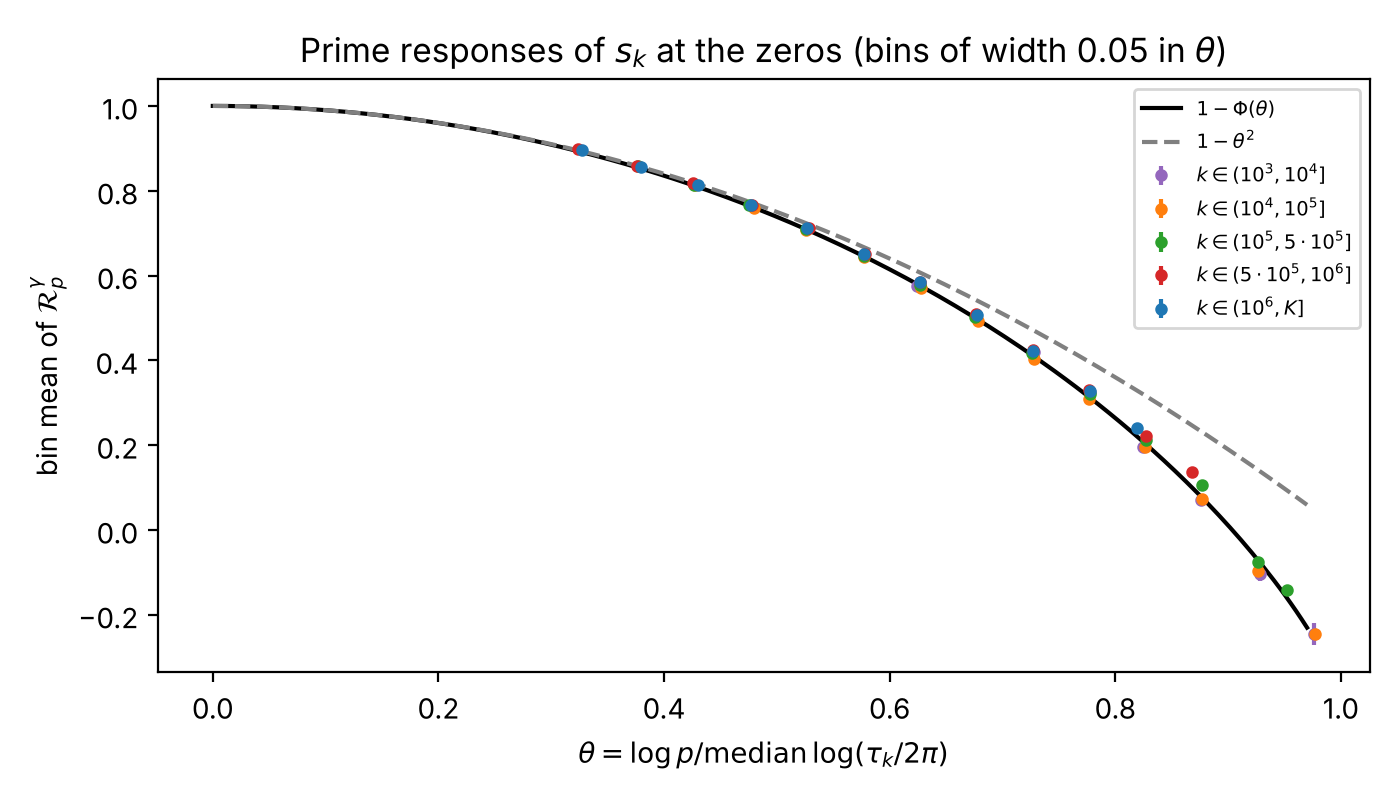
\includegraphics[width=0.86\textwidth]{fig07_response_law.png}
\caption{Bin means of $\Rg_p$ (bars: descriptive standard error, see the text) against $1-\Phi(\theta)$ (solid) and $1-\theta^2$ (dashed), for five windows of ordinals.}
\label{fig:response_law}
\end{figure}

\begin{figure}[htbp]
\centering
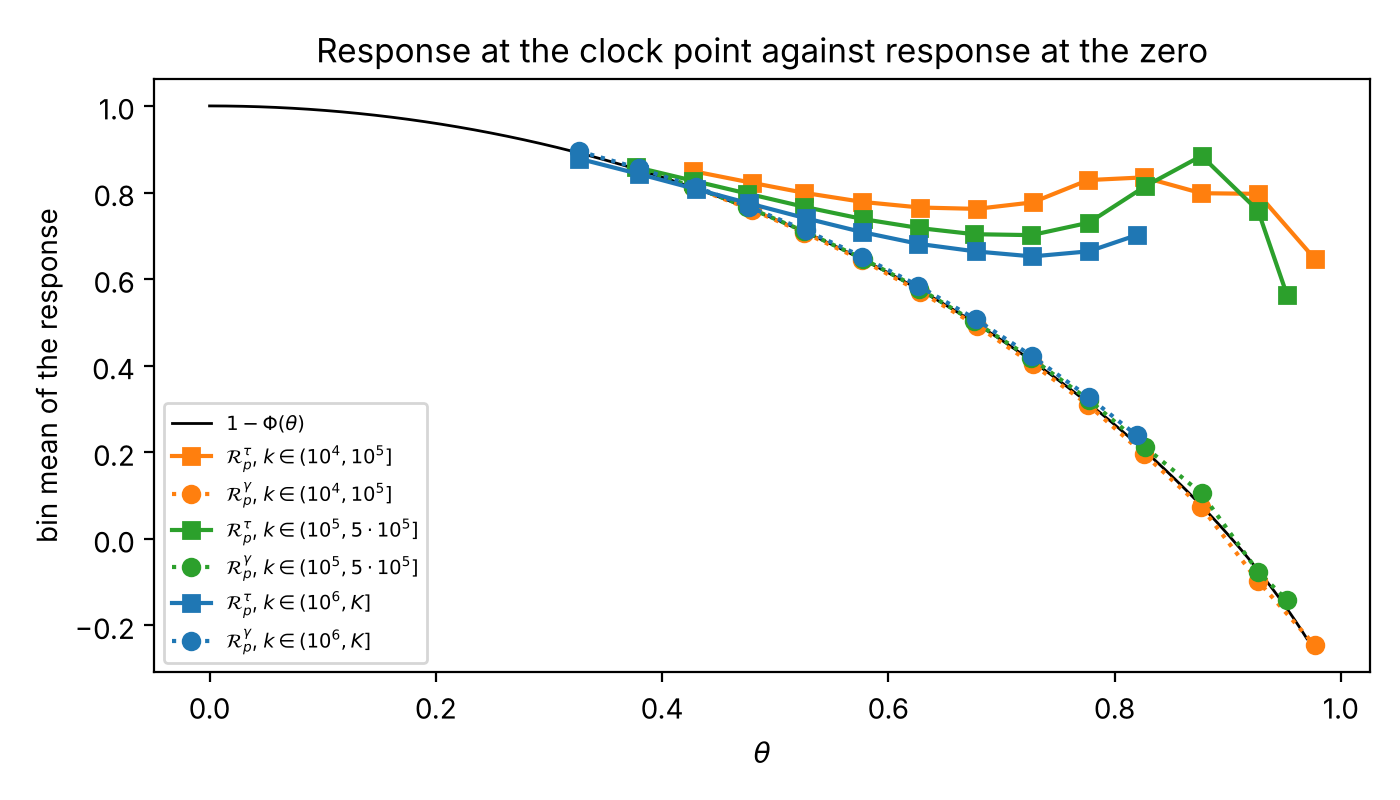
\includegraphics[width=0.86\textwidth]{fig08_response_clock_vs_zero.png}
\caption{Bin means of the response at the clock points, $\Rt_p$ (squares), and at the zeros, $\Rg_p$ (circles), for three windows of ordinals; solid: $1-\Phi(\theta)$.}
\label{fig:response_clock}
\end{figure}

The bin means follow $1-\Phi(\theta)$ and separate from $1-\theta^2$ for $\theta\ge0.6$. The residuals are not noise: in the two top windows every bin mean exceeds the candidate, by about $0.004$ at $\theta\approx0.3$ and $0.02$--$0.035$ at $\theta\approx0.8$--$0.9$, many standard errors. In every bin the excess is smaller in the top window than in the preceding one, by $6$--$23\%$; since $\theta$ is computed with the median height of each window, a bin contains different primes in the two windows, and two windows do not determine a rate of decay. The data are consistent with Conjecture~\CGref{conj:law} only together with a finite-height correction of a few hundredths. The standard errors treat the primes of a bin as independent; since all responses are computed on the same ordinates, they are descriptive only. The response at the clock points follows a different curve, with a plateau near $0.65$--$0.70$ for $\theta\in[0.65,0.80]$ in the top window (Figure~\CGref{fig:response_clock}), as Remark~\CGref{rem:transport} allows.

%======================================================================
\section{Conclusions}
\label{sec:conclusions}

\subsection{What was known}
Before this work, the relation between the RvM clock and the ordinates of the zeros of the Riemann zeta function was known at two levels. Pointwise, $\delta_k=\tau_k-\gamma_k$ is bounded, with $\limsup|\delta_k|\le0.6331$ as an immediate consequence of the bound of Bellotti and Wong \cite{BellottiWong2025}. On average, $s_k$ is asymptotically Gaussian with variance $\frac1{2\pi^2}\log\log T$, by Selberg's formulae for the Gram displacement proved by Korolev \cite{Korolev2012,Korolev2011}, so $\langle\delta_k^2\rangle\sim2\log\log T/\log^2T$: the clock is close to the zeros in height, but it misplaces almost every zero by an unbounded number of positions. Selberg's approximation \cite{Selberg1946a,Fujii1974} replaces $S(t)$ by short prime sums in $t$-mean, and Fran\c{c}a--LeClair and LeClair \cite{FrancaLeClair2015,LeClair2021,FrancaLeClair2024} write the equation of an individual zero with an Euler phase and a growing number of primes, with computations at a fixed number of primes. Gram's law \cite{Gram1903} and Turing's method \cite{Turing1953} locate the zeros on the critical line between Gram points, with exceptions at about a quarter of the indices at the heights of the table.

\subsection{What this paper adds}
\begin{enumerate}[leftmargin=1.6em]
\item \emph{An exact dictionary between clock-type models and the zeros} (Theorems~\CGref{thm:identity_general} and \CGref{thm:identity_g}). For any $C^1$ model $F$ and any continuous $\mathfrak g$, sums of $\mathfrak g$-increments of $k-\frac12-F(\gamma_k)$ over the ordinates are exactly $dF$-integrals of $\mathfrak g(N-F)$ up to two boundary terms; for powers this gives the even moments with the constant $\frac1{12}$ per zero, for exponentials it transfers the signed law of $S(t)$ to $s_k$ (Corollary~\CGref{cor:signed_law}).
\item \emph{The prime information needed by the clock} (Theorems~\CGref{thm:main} and \CGref{thm:variable_cutoff}). The corrected clock equation $\NO(t)+S_X(t)=k-\frac12$ holds at the true ordinates with mean-square ordinal defect $\frac1{2\pi^2}\log\frac{\log T}{\log X}+O(1+\sqrt{\log(\log T/\log X)})$, also with a cutoff varying at every index; the defect is bounded in mean square if and only if the primes reach a fixed power of the height.
\item \emph{A computable clock that is closer to the zeros by an order of magnitude} (Theorems~\CGref{thm:computable_clock}, \CGref{thm:second_step} and \CGref{thm:uniform_iteration}). With $X=T^{1/\sqrt{\log\log T}}$ the one-step clock has mean-square error $(\log\log\log T+O(\sqrt{\log\log\log T}))/\log^2T$ in height, against $(2+o(1))\log\log T/\log^2T$ for the bare clock; the $m$-th Newton step has error $\frac{H_m}{4\pi^2}+O(1+\sqrt{H_m})$ in units of zeros with absolute constants, and after $\log^*T+O(1)$ steps the error is $O(1)$ mean spacings, using no ordinate. The proof needs an exact moment recursion, a multiplicity bound for the corrected points of every level (Theorem~\CGref{thm:multiplicity_all}) and a cutoff law that absorbs the multiplicity.
\item \emph{The pointwise envelope} (Proposition~\CGref{prop:envelope_equivalence}, Theorem~\CGref{thm:envelope}, Proposition~\CGref{prop:explicit_S}). $\limsup|\tau_k-\gamma_k|=2\pi\limsup|S(t)|/\log t$ exactly, no slowly growing prime correction changes it, and $\limsup|\tau_k-\gamma_k|<0.60832$.
\item \emph{An exact finite-height account, the prime responses and the transport identity} (Theorems~\CGref{thm:accounting} and \CGref{thm:twist}, Section~\CGref{sec:responses}). The gain of the one-step clock is a diagonal response minus a cross term; the cross term vanishes for $X\le T^{1/4-\varepsilon}$ and switches on at the Nyquist cutoff through pairs $pq\approx\tau/2\pi$ (Proposition~\CGref{prop:pair_resonance}); the prime phases at the clock points are almost orthonormal for $p\le T^{1-\varepsilon}$, which gives a spectral energy inequality; the twisted integral $\frac1T\int_T^{2T}p^{\,i(t+G/\lL)}dt$ is exactly a sum over the displacements at the clock points; the response of the moving primes $p=T^\theta$ is carried by the transport and the residual of the Newton steps (Theorem~\CGref{thm:computable_response}), and under two named hypotheses it is $1-\Phi(\theta)$.
\item \emph{Certified roots and continuation} (Lemmas~\CGref{lem:monotone_sharp} and \CGref{lem:certified_root}, Proposition~\CGref{prop:residual_identity}, Theorem~\CGref{thm:continuation}). The corrected equation is monotone for $M_{\le X}\le(1-\mathsf c)\lL$, with a criterion that is sharp uniformly in $t$; its root is found by bisection with no residual; the residual of a Newton step is separated exactly from the defect at the ordinate; and a root can be continued to any larger cutoff along a homotopy that cannot change branch, under a condition that is local to the segment between two consecutive roots and is not limited by $X\le T^{1/2}$. With a per-index cutoff rule that uses no ordinate, the continued roots improve the comparison array selected by validation in every measure on the $600\,316$ untouched indices (Table~\CGref{tab:rule}), and continued beyond the height in the scale $\tau/2\pi$ they reach a root mean square of $0.0128$ mean spacings in height on a block of $10\,000$ untouched indices, against $0.0403$ for the comparison array (Table~\CGref{tab:beyond_nyquist}).
\item \emph{Phase coherence} (Propositions~\CGref{prop:angular_radial}--\CGref{prop:quotient_modes}). The drift of the phase walk $\sum e^{ix_k}$ of corrected points has an exact angular/radial decomposition, and relative to the clock an exact split of its quadratic part into product and quotient modes. The quotient modes are bounded for a fixed set of prime powers, with period $\log(T/2\pi)/|1+\log(n_1/n_2)|$, and become slow when $n_2/n_1$ is close to $e$: the convergents $\frac83,\frac{11}4,\frac{19}7,\frac{193}{71}$ of $e$ whose two terms are prime powers. On the table one pair, $(71,193)$, carries $14.0$ of the drift $16.2$ of the comparison array.
\item \emph{Separation of the ordinates} (Proposition~\CGref{prop:isolated}, Theorem~\CGref{thm:local_separation}, Corollary~\CGref{cor:proportion}, Proposition~\CGref{prop:verification}). An ordinate isolated in the list counted with multiplicity is a simple zero on the critical line. Zero-free points whose errors are smaller than half their gaps isolate the ordinates and force a sign change of $Z$ between consecutive midpoints; this gives a lower bound for the number of simple zeros on the line in terms of the mean square of a zero-free construction and of its own gaps, and a verification procedure in which the corrected points replace the Gram points. On the untouched indices the corrected Gram law fails at $0.019\%$ of the indices for the rule R2, against $24.3\%$ for Gram's law (Table~\CGref{tab:gram_law}).
\end{enumerate}

\subsection{Status of the proofs and pending verification}
\label{subsec:pending}
Every statement called Theorem, Proposition, Lemma or Corollary in Sections~\CGref{sec:identities}--\CGref{sec:separation} and \CGref{subsec:landau_line}--\CGref{subsec:newton_spectrum} is proved in the text from the external results of Section~\CGref{sec:known_results} and the results quoted where they are used. The following points are recorded so that a reader can check them independently.
\begin{enumerate}[leftmargin=1.6em]
\item \emph{External inputs read in the original.} Theorems~\CGref{thm:known_selberg_approx} and \CGref{thm:known_fujii_difference} (Fujii, pp.~225 and 232--233), \CGref{thm:known_korolev} (Korolev, Thm.~4.2, with his convention for the Gram points), \CGref{thm:known_maximal} (Kinnunen, Thm.~1.4, and Stein, Thm.~I.1 as quoted there), \CGref{thm:known_exponents} (Bourgain, Thm.~6 of arXiv:1408.5794v2; Ivi\'c, Lemma~2.8 and (7.57)), \CGref{thm:known_stationary}, \CGref{thm:known_vdC}, \CGref{thm:known_vdC_weighted} and \CGref{thm:known_vdC2} (Titchmarsh, Lemmas~4.6, 4.7, 4.10 and Theorem~5.9), \CGref{thm:known_density} (Titchmarsh, Thm.~9.19(C)), \CGref{thm:known_KL} (Graham--Kolesnik, Thm.~2.1), \CGref{thm:known_landau} (Gonek's formula as stated in Aryan, (1.1)), \CGref{thm:known_backlund} and \CGref{thm:known_BW} (Bellotti--Wong, numbering of arXiv:2412.15470v2). Theorem~\CGref{thm:known_carleson} is taken from Lerner's statement for the real line. The following are cited as stated in those sources: Carleson's and Hunt's papers, Billingsley's Theorems~26.3 and 30.2, Folland's \S3.5, Soshnikov's cumulant formula, Jacobi's expansion in Watson's treatise, Tsang's thesis (through \cite{FazzariGerspachMinelli2025}), Kronecker's theorem \cite{HardyWright2008}, the continued fraction of $e$ \cite{Olds1970}, Hardy's function and the symmetry of the zeros \cite{Titchmarsh1986}, Gram's law \cite{Gram1903}, Turing's method \cite{Turing1953}, the verification of the Riemann hypothesis to height $3\cdot10^{12}$ \cite{PlattTrudgian2021}, the positive proportions \cite{Selberg1942,PrattRoblesZaharescuZeindler2020}, and the semiclassical results of Section~\CGref{subsec:routes_casana} \cite{Berry1988,BogomolnyKeating1995,BogomolnyKeating1996PRL,BogomolnyKeating1996,HardyLittlewood1923}.
\item \emph{Constants in the moment order.} Lemmas~\CGref{lem:higher_moments} and \CGref{lem:sampling_rho} carry explicit dependence on the moment order $r$; Theorem~\CGref{thm:uniform_iteration} uses them with $r$ up to $2^m$, $m\le\log^*T+O(1)$. The constants $C_\star$, $H^*$, $B_\star$, $C_6$, $C'$ are absolute and not computed; the statement is asymptotic in $T$.
\item \emph{Proposition~\CGref{prop:explicit_S}.} The explicit constants $10$, $30$, $|\chi(\sigma+it)|\le3t^{1/2-\sigma}$, $R(T)<1$ and the interval-arithmetic values of $I/(2\pi D)$ and $1/(2D)$ come from a computation communicated to the author and have not been recomputed; the coefficient $0.09783$ agrees with \texttt{opc\_envelope\_coefficient\_v14.py}.
\item \emph{Propositions~\CGref{prop:resonance} and \CGref{prop:pair_resonance}.} In \CGeqref{eq:cross_term_pairs} the non-resonant error term is crude; the agreement of Section~\CGref{subsec:onset} to $0.02\%$ is better than what is proved at that height. Remark~\CGref{rem:product_modes} is a stationary-phase evaluation with the same status.
\item \emph{Corollaries~\CGref{cor:weighted_response} and \CGref{cor:unweighted}.} The passage from the weighted response to $\Rt_p$ is proved for $p\le(\log T)^{4-\varepsilon}$ and not for $p=T^\theta$.
\item \emph{The certificates of Section~\CGref{subsec:rule_data}.} Theorem~\CGref{thm:continuation} is proved; its hypothesis was checked by the programs at five (Table~\CGref{tab:rule}) or three (Table~\CGref{tab:beyond_nyquist}) points of each segment between consecutive roots, not by interval arithmetic or with a bound for $F''$. The continued roots are therefore numerical roots of the corrected equation reached by a continuation whose branch condition is sampled.
\item \emph{What is not proved.} The moving-prime law $1-\Phi(\theta)$ rests on Hypotheses U and W; the transfer estimate \CGeqref{eq:transfer_estimate} is open; a bounded error with a fixed cutoff (Remark~\CGref{rem:newton}) is open; the cutoff law \CGeqref{eq:cutoff_law} is not claimed to be optimal; Heuristic~\CGref{heur:gaussian_cutoff} is a model, and its value of $\hat\sigma$ exceeds the measured one; the decrease of the error of the continued roots as the cutoff exponent grows is observed on one block, and neither its limit nor its rate is proved.
\item \emph{Numerical statements.} All printed numbers are produced by the programs listed in Appendix~\CGref{app:programs} from the input files whose SHA-256 identifiers are given in the Data availability statement. Descriptive, with no asymptotic statement behind them: $\theta_{\rm fit}=0.5744$ and the minimizing cutoffs (Table~\CGref{tab:methods}); the standard errors of Figures~\CGref{fig:response_law}--\CGref{fig:response_clock}; the excess of $0.004$--$0.035$ over $1-\Phi(\theta)$; the plateau of $\Rt_p$; the correlations of Table~\CGref{tab:transport}; Table~\CGref{tab:iteration}; Table~\CGref{tab:computable_response}; the selection of the comparison array by validation; Tables~\CGref{tab:newton_residual_spectra}--\CGref{tab:gram_law}, the fits of Section~\CGref{subsec:beyond_nyquist} and the drift values of Section~\CGref{subsec:walk_data}. Comparisons with a proved statement: the resonant main term of Section~\CGref{subsec:onset}; the two resonance values of Table~\CGref{tab:twist}; $|I-D-J|\le2\cdot10^{-7}$; the envelope used to $66\%$ and $15\%$; Table~\CGref{tab:accounting}; the closures $3\cdot10^{-16}$ and $6\cdot10^{-14}$ of \CGeqref{eq:product_quotient} and \CGeqref{eq:angular_radial}; the implication of Theorem~\CGref{thm:local_separation}, checked at every index where its hypotheses hold. Data checks: the spot checks against \texttt{mpmath.zetazero}, the clock certificate, $|\delta_{34}|=0.9937$, $\max_k|s_k|=1.3325$, and the reconstruction of the comparison array to $9.3\cdot10^{-10}$.
\end{enumerate}

\subsection{What is missing for a complete prediction of the zeros from the clock}
\label{subsec:missing}
Theorem~\CGref{thm:uniform_iteration} locates the ordinates from $\tau_k$ and the primes with a mean-square error of $O(1)$ mean spacings, and the continued roots of Section~\CGref{subsec:beyond_nyquist} reach about a hundredth of a spacing on the data. A complete prediction, assigning to each zero its index and position, requires the following; none is proved here.
\begin{enumerate}[leftmargin=1.6em]
\item \emph{From $O(1)$ to $o(1)$ in mean square} (Question~\CGref{q:fixed_c}). A correction computable from the clock and the primes that removes the residual of the final clock; by Proposition~\CGref{prop:spectral_energy} this is equivalent to reproducing the responses $\Rt_p$ of the moving primes in $L^2(dp/p)$, and by Theorem~\CGref{thm:computable_response} these responses are carried by the residual. The two routes known are the cancellation between transport and defect of Remark~\CGref{rem:newton} and the transfer estimate \CGeqref{eq:transfer_estimate}.
\item \emph{The constant of Theorem~\CGref{thm:main}} (Question~\CGref{q:constant}). Assigning indices needs a final mean square below $\frac14$ in units of zeros; for cutoffs near $T^{1/2}$ the question is the value of Selberg's constant $C$.
\item \emph{Cutoffs $X>T^{1/2}$.} Theorem~\CGref{thm:main}, Theorem~\CGref{thm:known_MV} and the moment lemmas require $X^2\le T$. Theorem~\CGref{thm:continuation} is not restricted, and the data of Table~\CGref{tab:beyond_nyquist} go to $X=(\tau/2\pi)^{1.30}$; a mean-square theorem in this range is missing.
\item \emph{Pointwise control.} Everything proved is in mean square. A zero-by-zero prediction needs at least the hypotheses of Theorem~\CGref{thm:local_separation} outside $o(\#\IT)$ indices, and the moment method does not reach them.
\item \emph{The moving-prime law.} By item~1 it is the same arithmetic: if the residual carries the response of the moving primes, the function $\rho^\tau(\theta)$, if it exists, is the spectrum of what is missing.
\end{enumerate}

\subsection{Why a finer knowledge of $\tau_k-\gamma_k$ matters}
The clock is the deterministic part of the ordinates, and $\delta_k$ carries all the arithmetic. Statistics of $\delta_k$ and $s_k$ are statistics of the zeros that do not depend on an unfolding of the ordinates or on Gram intervals. Theorem A turns questions about the ordinates into questions about $N-F$ in $t$-mean, so any improvement of the $t$-mean description of $S(t)$ passes to the zeros. Theorem D and Proposition~\CGref{prop:residual_identity} show that the error of a computable clock is governed by three separate quantities: the prime information missing below the cutoff (Theorem B), the transport between the computable point and the ordinate, whose observed anticorrelation with the defect (Table~\CGref{tab:transport}) is not explained by any proved estimate, and the residual of the equation, which certified roots remove. Pointwise, Proposition~\CGref{prop:envelope_equivalence} identifies the extreme displacement of the clock with the extreme size of $S(t)$, and Theorem~\CGref{thm:local_separation} turns errors smaller than half the computed gaps into simple zeros on the critical line. The measured responses $\Rt_n$, $\Rg_n$, the cross terms $\Cr_X$ and the drift of the walk are exact finite-height invariants of the zeros, which any model of the zeros must reproduce.

\subsection{Future work}
\begin{question}\label{q:constant}
For fixed $c\in(0,\frac12]$, do the bounded means of $u_k(T^c)^2$ converge, and to $(2\pi^2)^{-1}\log(1/c)$ plus which constant?
\end{question}

\begin{question}\label{q:fixed_c}
Does $\langle r_k(T^c)^2\rangle_{\IT}$ stay bounded for fixed $c$, that is, does the transport cancel against the defect as in Table~\CGref{tab:transport}? Is the error of the corrected clock after $\log^*T+O(1)$ steps bounded in units of zeros for \emph{almost every} index, and not only in mean square? Can Theorems~\CGref{thm:main} and \CGref{thm:computable_clock} be extended to $c>\frac12$?
\end{question}

\begin{question}\label{q:prime_bridge}
Can Hypotheses~U and W be proved for $p=T^\theta$, that is, can the terms of Proposition~\CGref{prop:PY_square} that contain Selberg's remainder be evaluated to $o(p^{-1/2})$? What is the finite-height correction to $1-\Phi(\theta)$ seen in Table~\CGref{tab:response_bins}?
\end{question}

\begin{question}\label{q:floor}
For the roots of $F_{\le Y}=k-\frac12$ continued from the certified root to $Y=(\tau_k/2\pi)^c$, does the mean-square error in units of zeros tend to $0$ as $c$ grows, or to a positive floor? For which proportion of the indices does the branch condition of Theorem~\CGref{thm:continuation} hold up to a given $c$?
\end{question}

\begin{question}\label{q:pair_newton}
Is there a correction step beyond $T^{1/2}$, built on pairs of prime powers with Hardy--Littlewood weights, whose mean square in units of zeros is $o(1)$?
\end{question}

\begin{question}\label{q:corrected_gram_law}
For which proportion of $k\in\IT$ does the corrected Gram law $Z(\bar x_{k-1})Z(\bar x_k)<0$ hold for a zero-free construction, and can a positive proportion be proved from Theorem~\CGref{thm:uniform_iteration} with explicit constants and Corollary~\CGref{cor:proportion}?
\end{question}

\begin{question}\label{q:excess}
What is the shape of the excess-root count $\mathcal N^{\rm ex}(Y,T)$ of \CGeqref{eq:excess} as a function of $\log Y/\log T$, and does it tend to zero along a continuation?
\end{question}

\begin{question}\label{q:e_convergents}
Is there a correction of the quotient modes $n_2/n_1\approx e$, computable from the clock and the primes, which removes the drift of the walk of the corrected points without increasing their mean-square error?
\end{question}

Theorem~\CGref{thm:identity_general} applies to any counting staircase and any $C^1$ model, in particular to the zeros of a primitive Dirichlet $L$-function; an analogue of Theorem~\CGref{thm:main} would additionally need Selberg's approximation for $L(s,\chi)$ \cite{Selberg1946b,Fujii1974} and uniformity in the conductor.

\subsection{Routes towards the Casa\~na Law}
\label{subsec:routes_casana}
We call \emph{Casa\~na Law} a method that, starting from $\tau_k$ and using only the primes, produces points $x^{[m]}_k$ with
\begin{equation}
\gamma_k=\lim_{m\to\infty}x^{[m]}_k ,
\label{eq:casana_law}
\end{equation}
each $x^{[m]}_k$ computed from $k$, $\tau_k$ and finitely many prime powers, by a rule that does not depend on any ordinate. Theorem~\CGref{thm:uniform_iteration} gives an error $O(1)$ in mean square; the continued roots give about $0.013$ mean spacings in height on the data. The following routes start from the results above; none is carried out here.

\paragraph{The staircase limit} At an ordinate, $u_k(A)=S^*(\gamma_k)-S_A(\gamma_k)+\varpi(\gamma_k)/\pi$ (Section~\CGref{subsec:euler_phase}), so by Proposition~\CGref{prop:residual_identity} the certified root of $F_{\le Y}=k-\frac12$ satisfies $|x_k-\gamma_k|\le|u_k(A_{\le Y})|/\mathsf d$ whenever $F_{\le Y}'\ge\mathsf d$ between $x_k$ and $\gamma_k$. The equation \CGeqref{eq:casana_law} therefore holds along a sequence of cutoffs $Y_m(k)$ if
\begin{equation}
S_{\le Y_m(k)}(\gamma_k)\longrightarrow S^*(\gamma_k)+\frac{\varpi(\gamma_k)}\pi\qquad\text{and}\qquad\inf F'_{\le Y_m(k)}\ \text{on the segment stays}\ \gg\lL(\tau_k),
\label{eq:staircase_limit}
\end{equation}
that is, if the corrected count converges at the ordinate to the midpoint of the step of the counting function, and its slope near the ordinate does not degenerate. The model of this limit is the staircase $N-\varpi/\pi$, which is monotone and has the value $k-\frac12$ exactly at the middle of its $k$-th step. The Euler phase does not converge on the critical line, and Selberg's approximation controls $S-S_Y$ only in $t$-mean and for $Y\le T$; \CGeqref{eq:staircase_limit} at the ordinates, for $Y$ beyond the height, is the open point. The data of Table~\CGref{tab:beyond_nyquist} follow \CGeqref{eq:staircase_limit} up to $Y=(\tau/2\pi)^{1.30}$, with a decrease that slows down (Question~\CGref{q:floor}).

\paragraph{Pairs of primes beyond $T^{1/2}$} Beyond the Nyquist cutoff the primes no longer act one at a time: the obstruction of Theorem~\CGref{thm:computable_response} is the pair resonance $pq\approx T/2\pi$. In the semiclassical description of the zeros \cite{Berry1988,BogomolnyKeating1995,BogomolnyKeating1996PRL,BogomolnyKeating1996} this is the off-diagonal regime, $\tau=r\log p/\log(E/2\pi)>\tau^*$ in the notation of \cite[(13)--(21)]{Berry1988}, where the contributions of pairs of primes are evaluated through the Hardy--Littlewood prime-pair conjecture \cite{HardyLittlewood1923} and produce the GUE correlations \cite{BogomolnyKeating1996}. A correction beyond $T^{1/2}$ that reduces the mean square to $o(1)$ would therefore contain a term built on pairs of prime powers with Hardy--Littlewood weights, and not only further single primes (Question~\CGref{q:pair_newton}).

\paragraph{The branch condition} Theorem~\CGref{thm:continuation} turns the limit \CGeqref{eq:casana_law} into a condition on the corrected equation alone: the slope $F'_{\le Y}$ must stay positive on the segments between consecutive roots of the ladder. The condition fails when $F_{\le Y}$ develops excess roots near the level $k-\frac12$; with
\begin{equation}
\mathcal N^{\rm ex}(Y,T)=\#\bigl\{t\in(T,2T]:\ F_{\le Y}(t)\in\mathbb Z+\tfrac12\bigr\}-\#\IT
\label{eq:excess}
\end{equation}
one has $\mathcal N^{\rm ex}(Y,T)=0$ up to boundary terms for $M_{\le Y}<\lL(T)$ (Lemma~\CGref{lem:monotone_sharp}). The excess is the obstruction to the continuation, and its decrease for large $Y$ would be the monotonicity of the staircase limit (Question~\CGref{q:excess}). On the data the branch condition fails at fewer than $0.1\%$ of the indices at each level up to $Y=(\tau/2\pi)^{1.30}$.

\paragraph{The scale of the error without zeros} The cutoff of Heuristic~\CGref{heur:gaussian_cutoff} needs the error of the previous stage in units of zeros. The model value $\hat\sigma$ is computed from the omitted prime powers; the measured value is smaller. A self-consistent rule replaces $\hat\sigma$ by the size of the corrections of the continuation, $\lL(\tau_k)|x^{\rm A}_k-x_k|$, which is computable; with it the gain rule of Heuristic~\CGref{heur:gaussian_cutoff} has no fixed point below $c=1$ at the heights of the table (header of \texttt{opc\_task4\_selfconsistent\_cutoff.py}), which is the regime of Table~\CGref{tab:beyond_nyquist}.

\paragraph{The alternation and the Nyquist cutoff} The alternation of the residual at lag $1$ is the folded defect of the prime powers just above the final cutoff (Remark~\CGref{rem:nyquist}). Stopping at $X=(\tau/2\pi)^{1/2}$ puts its frequency at $\frac12$; crossing the Nyquist cutoff moves it to $1-c<\frac12$ and reduces it (Tables~\CGref{tab:rule} and \CGref{tab:beyond_nyquist}), and it disappears only when the defect $u_k$ does.

\paragraph{The walk as a consequence} The walk of the ordinates is not used in any construction. A Casa\~na Law must reproduce it: by Proposition~\CGref{prop:quotient_modes} the quotient modes with $n_2/n_1$ a convergent of $e$ have periods that grow without bound with the cutoff, and in the walk of the zeros their contributions cancel (Section~\CGref{subsec:walk_data}). A construction whose walk drifts is not converging to the ordinates in the coherent sense, whatever its mean-square error; the cancellation of these modes must come out of the construction, not be imposed on it (Question~\CGref{q:e_convergents}).

\subsection{Routes towards the Riemann hypothesis}
\label{subsec:routes_rh}
By Proposition~\CGref{prop:isolated}, all zeros up to height $t$ are simple and lie on the critical line if and only if the ordinates up to $t$, counted with multiplicity, are distinct, and if and only if $Z$ has $N(t)$ sign changes in $(0,t]$. Every route below produces sign changes of $Z$, or isolated ordinates, at points computed without zeros; $N(t)$ is computable by the Riemann--von Mangoldt formula and Turing's method \cite{Turing1953}. None of them is carried out here; their status is stated with each.

\paragraph{Route 1: the corrected Gram law at every index} If $Z(\bar x_{k-1})Z(\bar x_k)<0$ for $k_1<k\le k_2$ and $N(\bar x_{k_2})-N(\bar x_{k_1})=k_2-k_1$, all zeros in $(\bar x_{k_1},\bar x_{k_2})$ are simple and on the line (Proposition~\CGref{prop:verification}). At finite height this is a verification method whose exceptions are those of the corrected law: $0.019\%$ of the indices for R2 and none on the block with $c\ge1$, against $24.3\%$ for Gram's law (Table~\CGref{tab:gram_law}). The asymptotic statement needs the law for every index, which is a pointwise statement about $S(t)$ at the computable midpoints (Proposition~\CGref{prop:envelope_equivalence}).

\paragraph{Route 2: errors below half the computed gaps} By Theorem~\CGref{thm:local_separation}, if a zero-free construction satisfies
\begin{equation}
|x_j-\gamma_j|<\mathsf h_k\quad(j=k-1,k,k+1),\qquad\min(x_k-x_{k-1},x_{k+1}-x_k)>2\mathsf h_k\qquad\text{for every }k,
\label{eq:route_separation}
\end{equation}
for some $\mathsf h_k>0$, then all ordinates are isolated and the Riemann hypothesis holds, with all zeros simple. The first condition concerns the error, the second only the construction. A Casa\~na Law with a pointwise rate does not suffice by itself: the error must be compared with the gaps of the construction at the same index, and the gaps of the ordinates, hence of any good construction, become arbitrarily small. The data show that the ratio is favourable at almost all indices: $99.6\%$ of the indices of the block satisfy \CGeqref{eq:route_separation} with $\mathsf h_k=0.1/\lL(\tau_k)$ for $c=1.30$.

\paragraph{Route 3: a positive proportion from the mean square} Corollary~\CGref{cor:proportion} with the clock corrected $m^*$ times gives the lower bound \CGeqref{eq:proportion_iteration} for the proportion of simple zeros on the line, in terms of the constant $C'$ of Theorem~\CGref{thm:uniform_iteration} and of the proportion of small gaps of the corrected points. Both are questions about zero-free objects: an explicit $C'$ and the gap distribution of $x^{(m^*)}_k$. A proportion above $\frac5{12}$ \cite{PrattRoblesZaharescuZeindler2020} would follow if the bracket in \CGeqref{eq:proportion_iteration} exceeds $\frac5{12}$; whether this is reachable is open (Question~\CGref{q:corrected_gram_law}).

\paragraph{Route 4: uniqueness of the root} Fran\c{c}a and LeClair write the equation of the $k$-th zero as $\NO(x)+\frac1\pi\lim_{\delta\to0^+}\arg\zeta(\frac12+\delta+ix)=k-\frac12$ and observe that, if it has a unique solution for every $k$, the solutions account for all zeros, which then lie on the critical line \cite{FrancaLeClair2015}.% VERIFICAR: section and page of this statement in FrancaLeClair2015
 For finite cutoffs, uniqueness is exactly what Lemma~\CGref{lem:monotone_sharp} certifies below $X_{\rm mon}$ and Theorem~\CGref{thm:continuation} propagates above it: the continued root is the unique root on its segment, reached without change of branch. The route is the continuation to arbitrarily large cutoffs with the branch condition, combined with Route 2 to identify the limit; its obstruction is the excess-root count \CGeqref{eq:excess}, which measures the failure of uniqueness, and the absence of a uniform lower bound for $F'_{\le Y}$ as $Y$ grows.

\paragraph{Route 5: the walk as a necessary condition} If $x^{[m]}_k\to\gamma_k$ for every $k\le K$, then $\mathscr C_K(x^{[m]})\to\mathscr C_K(\gamma)$, so a Casa\~na Law reproduces the walk of the ordinates. For the truncated constructions the quotient modes of Proposition~\CGref{prop:quotient_modes} with $n_2/n_1$ close to $e$ produce a drift that the mean square does not see (Section~\CGref{subsec:walk_data}); their contributions $\mathscr R_{n_1,n_2}$ are computable without zeros, and their cancellation in the limit is a necessary condition for Routes 1, 2 and 4. It does not by itself give sign changes of $Z$.

\section*{Declaration of competing interest}
The author declares no competing interests.

\section*{Data availability}
All programs, the input-generation script with its certificates, the numerical outputs (CSV, JSON and text) and the figures are in the public GitHub repository \url{https://github.com/vcasana1/LawCasanya}: all programs are in \texttt{work/v15/code/}; the outputs of Sections~\CGref{subsec:data}--\CGref{subsec:onset} and \CGref{sec:responses}--\CGref{sec:heuristic} are in \texttt{outputs/}, those of Sections~\CGref{subsec:zcasanya_data}--\CGref{subsec:gram_data} in \texttt{work/v15\_prep/outputs/} and \texttt{work/v15/outputs/}. The ordinates are Odlyzko's table \cite{OdlyzkoTables}; the two input files (arrays of $2\,001\,052$ little-endian double-precision numbers) are regenerated from that table by \texttt{make\_inputs\_v14.py}. Their SHA-256 identifiers are\\
\texttt{fafb9436ce6a506de58c96c9bc9765d3\allowbreak 942de3f15c921e99e0015b3e945fe0ac} (ordinates) and\\
\texttt{b4c6758f0aef3724d3345f894ff82d5b\allowbreak bcb0f6139025b8b266091f713faa9504} (clock). The comparison array \texttt{zCasanya.bin} of Section~\CGref{subsec:zcasanya_data} has SHA-256\\
\texttt{64d1de134e920c1eb89f61ba5d93c7f9\allowbreak 49b343bfa0d9ebf5da6fb647c2d790d9} and is reproduced from the clock by \texttt{opc\_rebuild\_zcasanya\_v15.py}. The computations used Python 3.13.16, NumPy 2.5.3, SciPy 1.18.1, Matplotlib 3.11.2 and mpmath 1.3.0.

\section*{Declaration of generative AI and AI-assisted technologies in the writing process}
During the preparation of this work the author used an AI assistant (Claude, Anthropic) to edit the text, check proofs and write analysis programs. The author reviewed and edited the content and takes full responsibility for it.

%======================================================================
\begin{thebibliography}{99}

\bibitem{Aryan2022}
F. Aryan, On an extension of the Landau--Gonek formula, J. Number Theory 233 (2022) 389--404, \href{https://doi.org/10.1016/j.jnt.2021.06.015}{https://doi.org/10.1016/j.jnt.2021.06.015}.

\bibitem{BellottiWong2025}
C. Bellotti, P.-J. Wong, Improved estimates for the argument and zero-counting function of the Riemann zeta-function, Math. Comp. (2025) (statements numbered as in arXiv:2412.15470v2), \href{https://doi.org/10.1090/mcom/4133}{https://doi.org/10.1090/mcom/4133}.

\bibitem{Berry1988}
M.V. Berry, Semiclassical formula for the number variance of the Riemann zeros, Nonlinearity 1 (3) (1988) 399--407, \href{https://doi.org/10.1088/0951-7715/1/3/001}{https://doi.org/10.1088/0951-7715/1/3/001}.

\bibitem{Billingsley1995}
P. Billingsley, Probability and Measure, third ed., Wiley, New York, 1995.

\bibitem{BogomolnyKeating1995}
E.B. Bogomolny, J.P. Keating, Random matrix theory and the Riemann zeros I: three- and four-point correlations, Nonlinearity 8 (6) (1995) 1115--1131, \href{https://doi.org/10.1088/0951-7715/8/6/013}{https://doi.org/10.1088/0951-7715/8/6/013}.

\bibitem{BogomolnyKeating1996}
E.B. Bogomolny, J.P. Keating, Random matrix theory and the Riemann zeros II: $n$-point correlations, Nonlinearity 9 (4) (1996) 911--935, \href{https://doi.org/10.1088/0951-7715/9/4/006}{https://doi.org/10.1088/0951-7715/9/4/006}.

\bibitem{BogomolnyKeating1996PRL}
E.B. Bogomolny, J.P. Keating, Gutzwiller's trace formula and spectral statistics: beyond the diagonal approximation, Phys. Rev. Lett. 77 (8) (1996) 1472--1475, \href{https://doi.org/10.1103/PhysRevLett.77.1472}{https://doi.org/10.1103/PhysRevLett.77.1472}.

\bibitem{Bourgain2017}
J. Bourgain, Decoupling, exponential sums and the Riemann zeta function, J. Amer. Math. Soc. 30 (1) (2017) 205--224 (theorems numbered as in arXiv:1408.5794v2), \href{https://doi.org/10.1090/jams/860}{https://doi.org/10.1090/jams/860}.

\bibitem{Carleson1966}
L. Carleson, On convergence and growth of partial sums of Fourier series, Acta Math. 116 (1966) 135--157, \href{https://doi.org/10.1007/BF02392815}{https://doi.org/10.1007/BF02392815}.

\bibitem{Corless1996}
R.M. Corless, G.H. Gonnet, D.E.G. Hare, D.J. Jeffrey, D.E. Knuth, On the Lambert $W$ function, Adv. Comput. Math. 5 (1996) 329--359, \href{https://doi.org/10.1007/BF02124750}{https://doi.org/10.1007/BF02124750}.

\bibitem{FazzariGerspachMinelli2025}
A. Fazzari, M. Gerspach, P. Minelli, Selberg's central limit theorem weighted by linear statistics of zeta zeros, preprint, arXiv:2507.04150, 2025, \href{https://doi.org/10.48550/arXiv.2507.04150}{https://doi.org/10.48550/arXiv.2507.04150}.

\bibitem{Folland1999}
G.B. Folland, Real Analysis: Modern Techniques and Their Applications, second ed., Wiley, New York, 1999.

\bibitem{FrancaLeClair2014}
G. Fran\c{c}a, A. LeClair, Statistical and other properties of Riemann zeros based on an explicit equation for the $n$-th zero on the critical line, preprint, arXiv:1307.8395, 2013, \href{https://doi.org/10.48550/arXiv.1307.8395}{https://doi.org/10.48550/arXiv.1307.8395}.

\bibitem{FrancaLeClair2015}
G. Fran\c{c}a, A. LeClair, Transcendental equations satisfied by the individual zeros of Riemann $\zeta$, Dirichlet and modular $L$-functions, Commun. Number Theory Phys. 9 (1) (2015) 1--50, \href{https://doi.org/10.4310/CNTP.2015.v9.n1.a1}{https://doi.org/10.4310/CNTP.2015.v9.n1.a1}.

\bibitem{FrancaLeClair2024}
G. Fran\c{c}a, A. LeClair, A theory for the zeros of Riemann $\zeta$ and other $L$-functions (updated), preprint, arXiv:1407.4358v2, 2024, \href{https://doi.org/10.48550/arXiv.1407.4358}{https://doi.org/10.48550/arXiv.1407.4358}.

\bibitem{Fujii1974}
A. Fujii, On the zeros of Dirichlet $L$-functions. I, Trans. Amer. Math. Soc. 196 (1974) 225--235, \href{https://doi.org/10.1090/S0002-9947-1974-0349603-2}{https://doi.org/10.1090/S0002-9947-1974-0349603-2}.

\bibitem{Gonek1993}
S.M. Gonek, An explicit formula of Landau and its applications to the theory of the zeta-function, in: A Tribute to Emil Grosswald: Number Theory and Related Analysis, Contemp. Math., vol. 143, Amer. Math. Soc., Providence, RI, 1993, pp. 395--413, \href{https://doi.org/10.1090/conm/143/1210528}{https://doi.org/10.1090/conm/143/1210528}.

\bibitem{GrahamKolesnik1991}
S.W. Graham, G. Kolesnik, Van der Corput's Method of Exponential Sums, London Math. Soc. Lecture Note Ser., vol. 126, Cambridge University Press, Cambridge, 1991, \href{https://doi.org/10.1017/CBO9780511661976}{https://doi.org/10.1017/CBO9780511661976}.

\bibitem{Gram1903}
J.-P. Gram, Note sur les z\'eros de la fonction $\zeta(s)$ de Riemann, Acta Math. 27 (1903) 289--304, \href{https://doi.org/10.1007/BF02421310}{https://doi.org/10.1007/BF02421310}.% VERIFICAR

\bibitem{HardyLittlewood1923}
G.H. Hardy, J.E. Littlewood, Some problems of `Partitio numerorum'; III: On the expression of a number as a sum of primes, Acta Math. 44 (1923) 1--70, \href{https://doi.org/10.1007/BF02403921}{https://doi.org/10.1007/BF02403921}.

\bibitem{HardyWright2008}
G.H. Hardy, E.M. Wright, An Introduction to the Theory of Numbers, sixth ed., revised by D.R. Heath-Brown and J.H. Silverman, Oxford University Press, Oxford, 2008.

\bibitem{HasanalizadeShenWong2022}
E. Hasanalizade, Q. Shen, P.-J. Wong, Counting zeros of the Riemann zeta function, J. Number Theory 235 (2022) 219--241, \href{https://doi.org/10.1016/j.jnt.2021.06.032}{https://doi.org/10.1016/j.jnt.2021.06.032}.

\bibitem{Hunt1968}
R.A. Hunt, On the convergence of Fourier series, in: Orthogonal Expansions and their Continuous Analogues (Proc. Conf., Edwardsville, Ill., 1967), Southern Illinois Univ. Press, Carbondale, 1968, pp. 235--255.

\bibitem{Ivic1985}
A. Ivi\'c, The Riemann Zeta-Function, Wiley, New York, 1985 (reprinted by Dover, Mineola, NY, 2003).

\bibitem{Kinnunen1997}
J. Kinnunen, The Hardy--Littlewood maximal function of a Sobolev function, Israel J. Math. 100 (1997) 117--124, \href{https://doi.org/10.1007/BF02773636}{https://doi.org/10.1007/BF02773636}.

\bibitem{Korolev2011}
M. Korolev, Gram's law and the argument of the Riemann zeta function, Publ. Inst. Math. (Beograd) (N.S.) 92(106) (2012) 53--78, \href{https://doi.org/10.2298/PIM1206053K}{https://doi.org/10.2298/PIM1206053K}.

\bibitem{Korolev2012}
M.A. Korolev, On Gram's law in the theory of the Riemann zeta function, Izv. Math. 76 (2) (2012) 275--309, \href{https://doi.org/10.1070/IM2012v076n02ABEH002583}{https://doi.org/10.1070/IM2012v076n02ABEH002583}.

\bibitem{Landau1912}
E. Landau, \"Uber die Nullstellen der Zetafunktion, Math. Ann. 71 (1912) 548--564, \href{https://doi.org/10.1007/BF01456808}{https://doi.org/10.1007/BF01456808}.

\bibitem{LeClair2021}
A. LeClair, Riemann hypothesis and random walks: the zeta case, Symmetry 13 (11) (2021) 2014, \href{https://doi.org/10.3390/sym13112014}{https://doi.org/10.3390/sym13112014}.

\bibitem{Lerner2013}
A.K. Lerner, On weighted norm inequalities for the Carleson operator, preprint, arXiv:1310.3352, 2013, \href{https://doi.org/10.48550/arXiv.1310.3352}{https://doi.org/10.48550/arXiv.1310.3352}.

\bibitem{Littlewood1924}
J.E. Littlewood, On the zeros of the Riemann zeta-function, Proc. Cambridge Philos. Soc. 22 (1924) 295--318, \href{https://doi.org/10.1017/S0305004100014225}{https://doi.org/10.1017/S0305004100014225}.

\bibitem{Mertens1874}
F. Mertens, Ein Beitrag zur analytischen Zahlentheorie, J. Reine Angew. Math. 78 (1874) 46--62, \href{https://doi.org/10.1515/crll.1874.78.46}{https://doi.org/10.1515/crll.1874.78.46}.

\bibitem{MontgomeryVaughan1974}
H.L. Montgomery, R.C. Vaughan, Hilbert's inequality, J. Lond. Math. Soc. (2) 8 (1974) 73--82, \href{https://doi.org/10.1112/jlms/s2-8.1.73}{https://doi.org/10.1112/jlms/s2-8.1.73}.

\bibitem{OdlyzkoTables}
A.M. Odlyzko, Tables of zeros of the Riemann zeta function: the first 2,001,052 zeros, accurate to within $4\cdot10^{-9}$, \url{https://www-users.cse.umn.edu/~odlyzko/zeta_tables/}, accessed 17 October 2026.

\bibitem{Olds1970}
C.D. Olds, The simple continued fraction expansion of $e$, Amer. Math. Monthly 77 (9) (1970) 968--974, \href{https://doi.org/10.2307/2318113}{https://doi.org/10.2307/2318113}.% VERIFICAR

\bibitem{PlattTrudgian2021}
D. Platt, T. Trudgian, The Riemann hypothesis is true up to $3\cdot10^{12}$, Bull. Lond. Math. Soc. 53 (3) (2021) 792--797, \href{https://doi.org/10.1112/blms.12460}{https://doi.org/10.1112/blms.12460}.% VERIFICAR

\bibitem{PrattRoblesZaharescuZeindler2020}
K. Pratt, N. Robles, A. Zaharescu, D. Zeindler, More than five-twelfths of the zeros of $\zeta$ are on the critical line, Res. Math. Sci. 7 (2020), Paper No. 2, \href{https://doi.org/10.1007/s40687-019-0199-8}{https://doi.org/10.1007/s40687-019-0199-8}.% VERIFICAR

\bibitem{Selberg1942}
A. Selberg, On the zeros of Riemann's zeta-function, Skr. Norske Vid.-Akad. Oslo I 1942 (10) (1942) 1--59.% VERIFICAR (no DOI)

\bibitem{Selberg1946a}
A. Selberg, Contributions to the theory of the Riemann zeta-function, Arch. Math. Naturvid. 48 (5) (1946) 89--155.

\bibitem{Selberg1946b}
A. Selberg, Contributions to the theory of Dirichlet's $L$-functions, Skr. Norske Vid.-Akad. Oslo I 1946 (3) (1946) 2--62.

\bibitem{Soshnikov2002}
A. Soshnikov, Gaussian limit for determinantal random point fields, Ann. Probab. 30 (1) (2002) 171--187, \href{https://doi.org/10.1214/aop/1020107764}{https://doi.org/10.1214/aop/1020107764}.

\bibitem{Stein1970}
E.M. Stein, Singular Integrals and Differentiability Properties of Functions, Princeton University Press, Princeton, NJ, 1970.

\bibitem{Tenenbaum2015}
G. Tenenbaum, Introduction to Analytic and Probabilistic Number Theory, third ed., Grad. Stud. Math., vol. 163, Amer. Math. Soc., Providence, RI, 2015, \href{https://doi.org/10.1090/gsm/163}{https://doi.org/10.1090/gsm/163}.

\bibitem{Titchmarsh1986}
E.C. Titchmarsh, The Theory of the Riemann Zeta-Function, second ed., revised by D.R. Heath-Brown, Clarendon Press, Oxford, 1986.

\bibitem{Trudgian2014}
T.S. Trudgian, An improved upper bound for the argument of the Riemann zeta-function on the critical line II, J. Number Theory 134 (2014) 280--292, \href{https://doi.org/10.1016/j.jnt.2013.07.017}{https://doi.org/10.1016/j.jnt.2013.07.017}.

\bibitem{Tsang1984}
K.-M. Tsang, The distribution of the values of the Riemann zeta-function, Ph.D. thesis, Princeton University, 1984.

\bibitem{Turing1953}
A.M. Turing, Some calculations of the Riemann zeta-function, Proc. Lond. Math. Soc. (3) 3 (1953) 99--117, \href{https://doi.org/10.1112/plms/s3-3.1.99}{https://doi.org/10.1112/plms/s3-3.1.99}.% VERIFICAR

\bibitem{Watson1944}
G.N. Watson, A Treatise on the Theory of Bessel Functions, second ed., Cambridge University Press, Cambridge, 1944.

\end{thebibliography}

\appendix
\section{Programs}
\label{app:programs}
The programs below are those of the repository (directory \texttt{work/v15/code/} and \texttt{work/v15/tools/}); each is reproduced verbatim. They run under Python 3 with NumPy, SciPy, Matplotlib and mpmath. The input files \texttt{zeross.bin} and \texttt{zLamb.bin} are produced by the first program from Odlyzko's table. The programs \texttt{opc\_common.py} and \texttt{opc\_task*.py} are run in a directory that contains \texttt{zeross.bin}, \texttt{zLamb.bin} and \texttt{zCasanya.bin} and write to its subdirectory \texttt{outputs/}; \texttt{opc\_task3\_analytic\_rule.py} runs first, \texttt{opc\_task4\_selfconsistent\_cutoff.py} is called with the target exponent (and the argument \texttt{1} for the single block), and the evaluation programs follow. The programs ending in \texttt{\_v15.py} locate the data through \texttt{opc\_common\_v15.py} and read the points of the \texttt{opc\_task*} programs from \texttt{work/v15\_prep/outputs/}.

\subsection{\texttt{make\_inputs\_v14.py}}
\proglisting{make_inputs_v14.py}

\subsection{\texttt{opc\_analysis\_v14.py}}
\proglisting{opc_analysis_v14.py}

\subsection{\texttt{opc\_checks\_v14.py}}
\proglisting{opc_checks_v14.py}

\subsection{\texttt{opc\_computable\_response\_v14.py}}
\proglisting{opc_computable_response_v14.py}

\subsection{\texttt{opc\_envelope\_check\_v14.py}}
\proglisting{opc_envelope_check_v14.py}

\subsection{\texttt{opc\_envelope\_coefficient\_v14.py}}
\proglisting{opc_envelope_coefficient_v14.py}

\subsection{\texttt{opc\_extensions\_v14.py}}
\proglisting{opc_extensions_v14.py}

\subsection{\texttt{opc\_iteration\_v14.py}}
\proglisting{opc_iteration_v14.py}

\subsection{\texttt{opc\_resonance\_v14.py}}
\proglisting{opc_resonance_v14.py}

\subsection{\texttt{opc\_transport\_v14.py}}
\proglisting{opc_transport_v14.py}

\subsection{\texttt{opc\_twist\_v14.py}}
\proglisting{opc_twist_v14.py}

\subsection{\texttt{opc\_validate\_v14.py}}
\proglisting{opc_validate_v14.py}

\subsection{\texttt{opc\_common.py}}
\proglisting{opc_common.py}

\subsection{\texttt{opc\_task1\_newton\_residual.py}}
\proglisting{opc_task1_newton_residual.py}

\subsection{\texttt{opc\_task2\_quotient\_drift.py}}
\proglisting{opc_task2_quotient_drift.py}

\subsection{\texttt{opc\_task3\_analytic\_rule.py}}
\proglisting{opc_task3_analytic_rule.py}

\subsection{\texttt{opc\_task4\_selfconsistent\_cutoff.py}}
\proglisting{opc_task4_selfconsistent_cutoff.py}

\subsection{\texttt{opc\_task4\_eval.py}}
\proglisting{opc_task4_eval.py}

\subsection{\texttt{opc\_task4\_eval\_b3.py}}
\proglisting{opc_task4_eval_b3.py}

\subsection{\texttt{opc\_task4\_fit\_b3.py}}
\proglisting{opc_task4_fit_b3.py}

\subsection{\texttt{opc\_common\_v15.py}}
\proglisting{opc_common_v15.py}

\subsection{\texttt{opc\_rebuild\_zcasanya\_v15.py}}
\proglisting{opc_rebuild_zcasanya_v15.py}

\subsection{\texttt{opc\_separation\_v15.py}}
\proglisting{opc_separation_v15.py}

\subsection{\texttt{opc\_walk\_centroids\_v15.py}}
\proglisting{opc_walk_centroids_v15.py}

\subsection{\texttt{opc\_e\_convergents\_v15.py}}
\proglisting{opc_e_convergents_v15.py}

\subsection{\texttt{tools/make\_tips\_v15.py}}
\proglisting{make_tips_v15.py}

\subsection{\texttt{tools/replace\_tips\_v15.py}}
\proglisting{replace_tips_v15.py}


\end{document}
